\cotefile{154}
\scanpage{77}
\deleted{\unsure{antipodique d'une}}

opposée d'une arête orientée $(D,\unsure{o|a})$ :
l'arête $(D',\unsure{o'|a'})$, où $D'$ est déduite de
$D$ par balayage via $\unsure{a'=\operatorname{antip}(a)}$,
et $\unsure{o'|a'}$ \deleted{\unsure{déduite de}} \inserted{\unsure{antipodale de celle}} $=$ par \uline{transport}
parallèle, i.e. ``opposée à $\unsure{o|a}$''.

Origine de $(D,\unsure{o|a})$ est $D$

2) Structure polygonale sur l'\unsure{ens.} des arêtes
orientées issues de $D$ : évidente

3) Transport d'orientations : \uuline{\unsure{opposé}}
du transport parallèle des orientations
des \unsure{f. p.}

Hélas on ne trouve pas les bons
circuits superréguliers --- \unsure{ça ne va pas}
\unsure{bien sûr}, si alléchant que celà
paraisse ! Si cependant on modifie
3), en prenant comme sens de transport
pour les orientations le transport parallèle,
on trouve les bons circuits \uline{superréguliers}
(mais pas d'application naturelle $\unsure{\mathcal X}\to X$ !).

Il y a une autre (au moins !) possibilité
de construction encore, c'est de \unsure{recoller} $a$ à $\unsure{b'}$,
$b$ à $a'$, ainsi

\figure{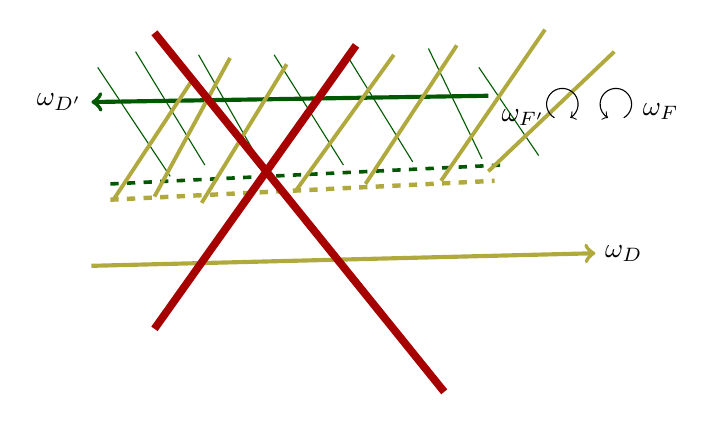
\begin{tikzpicture}[x=0.8cm,y=0.8cm]
\draw[green!35!black,line width=1.5pt,<-] (0,3.3)--(6.3,3.4);
\node[left] at (0,3.3) {$\omega_{D'}$};
\draw[yellow!65!black,line width=1.5pt,->] (0,0.7)--(8,0.9);
\node[right] at (8,0.9) {$\omega_D$};
\draw[green!35!black,line width=1.3pt,dashed] (0.3,2)--(6.5,2.3);
\draw[yellow!65!black,line width=1.6pt,dashed] (0.3,1.75)--(6.4,2.05);
\draw[green!35!black] (0.1,3.85)--(1.25,2.12);
\draw[green!35!black] (0.7,4.1)--(1.8,2.3);
\draw[green!35!black] (1.7,4.05)--(2.7,2.3);
\draw[green!35!black] (2.9,4.05)--(4,2.3);
\draw[green!35!black] (4.05,4.05)--(5.1,2.35);
\draw[green!35!black] (5.35,4.15)--(6.2,2.4);
\draw[green!35!black] (6.15,3.85)--(7.1,2.45);
\draw[yellow!65!black,line width=1.4pt] (0.35,1.75)--(1.6,3.65);
\draw[yellow!65!black,line width=1.4pt] (1,1.8)--(2.2,4);
\draw[yellow!65!black,line width=1.4pt] (1.75,1.7)--(3.1,3.9);
\draw[yellow!65!black,line width=1.4pt] (3.25,1.9)--(4.8,4.05);
\draw[yellow!65!black,line width=1.4pt] (4.35,2)--(5.8,4.2);
\draw[yellow!65!black,line width=1.4pt] (5.55,2.05)--(7.2,4.45);
\draw[yellow!65!black,line width=1.4pt] (6.3,2.2)--(8.3,4.1);
\draw[->] (7.35,3.05) arc[start angle=240,end angle=-60,radius=.25];
\node[left] at (7.35,3.05) {$\omega_{F'}$};
\draw[->] (8.45,3.05) arc[start angle=-60,end angle=240,radius=.25];
\node[right] at (8.6,3.15) {$\omega_F$};
\draw[red!65!black,line width=2.8pt] (1,4.4)--(5.6,-1.3);
\draw[red!65!black,line width=2.8pt] (1,-.3)--(4.2,4.2);
\end{tikzpicture}}

en utilisant pour le recollement le
transport parallèle, de façon donc
à avoir tjrs $\unsure{\mathcal X}\to X$, mais
cette fois pas une immersion,
mais \deleted{des} \unsure{applications|application} pliant
le long des arêtes de $K$.

La description combinatoire
est analogue à celle qui
précède, la seule modification
est dans 1) (description de
l'opposée d'une arête, \unsure{maint.} \inserted{\unsure{pour}}
l'opposée $(D',\unsure{o'|a'})$ de $(D,\unsure{o|a})$, $\unsure{o'|a'}$ est
déduite de $\unsure{o|a}$ par transport
parallèle. Pour $\unsure{2)\ \text{et}\ 3)}$, \unsure{ne rien changer}
\margin{\unsure{76}}
\scanpage{78}
Il s'ensuit que le quotient de
$\unsure{\mathcal X}$ par antipodisme est le $=$ que
précédemment, et que les suites de
\unsure{p.r.|p.v.} intervenant dans un circuit
sont les \inserted{mêmes} $\unsure{\Rightarrow|=}$ pour les deux --- donc
notre recette n'est pas plus satisfaisante,
en ce qui concerne les circuits
superréguliers ! Il faudrait modifier
3), en prenant la prescription opposée
pour définir le transport d'orientation,
pour trouver \deleted{\unsure{de}} bons circuits
superréguliers.

Qu'en serait-il dans le cas
où $\uline{\Sigma}$ est un syst. de \uline{droites} dans un
vrai plan projectif réel $X$ --- quand on regarde
le système de droites dans $X^\vee$ correspondant
aux sommets de $\Sigma$, i.e. les droites joignant
deux à deux les pts $\delta_i$ correspondant aux
droites $D_i$ ? On suppose \inserted{au besoin} que les $\delta_i$ sont non
alignés $3$ à $3$ (i.e. $\uline{\Sigma}\ \unsure{AdM}$), et que
les sommets \inserted{distincts des $\delta_i$} (de ce syst. de
$\frac{n(n-1)}2$ droites) sont simples (quitte
à perturber un peu le syst. des
$\delta_i$). Donc il n'y a que des
sommets d'ordre $4$, en dehors des
sommets ``\unsure{super-singuliers|superréguliers}'' $\delta_i$.

Considérons une face $F$ de $\uline{\Sigma}^\vee$,
qui définit donc une \unsure{p.r.|p.v.}
$D=D_F$, et considérons les
arêtes incidentes \inserted{$a_\alpha$ en $\overline F_\alpha=\Delta_\alpha\cap\overline F$} qui correspondent
à \uline{certaines} spécialisations
$D\to D_\alpha$ (où $\alpha$ est l'indice d'un
sommet de $\Sigma$, $\Delta_\alpha$ la droite
corr. dans $X^\vee$). Le sommet
$s_\alpha$ est le sommet d'un
tri. de spécialisation pour $D$,
soit $a'_\alpha$ l'arc de spécialisation,
correspondant. Je voudrais
\margin{77}
\scanpage{79}
interpréter la structure polygonale sur
l'ens des $a_\alpha$, en termes des $a'_\alpha$
correspondants. Notons déjà qu'il y
a correspondance entre les \deleted{\unsure{structures}} \inserted{orientations}
de $F$, et celles de $D$, et que le
transport continu de l'orientation de
$F$ vers une face adjacente $F'$
(le long de $a_\alpha$ disons) correspond au
transport continu (ou ``parallèle'') de
l'orientation de $D$ au cours du balayage
correspondant. \deleted{\unsure{(D}} Ce dernier point
rend plausible le choix ``naïf'' du
transport d'orientation, qui dans le contexte
des \unsure{modèles} de \unsure{p.v.} obtenus via balayage,
semble en effet meilleur, du pt de
vue ``circuits''. Le fait qu'on n'obtienne
pas d'application naturelle $\unsure{\mathcal X}\to X$ se
rapproche du fait qu'on n'a pas d'application
naturelle $X^\vee\to X$.

\figure{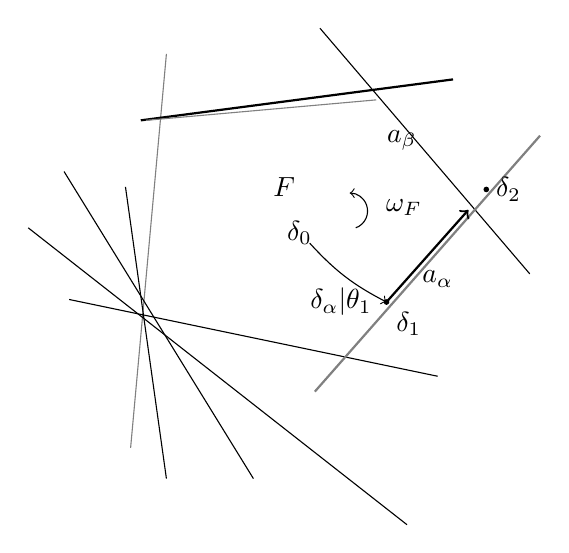
\begin{tikzpicture}[x=.65cm,y=.65cm]
\draw[gray] (1.8,0.8)--(2.5,8.5);
\draw (1.7,5.9)--(2.5,.2);
\draw (.5,6.2)--(4.2,.2);
\draw (-.2,5.1)--(7.2,-.7);
\draw (.6,3.7)--(7.8,2.2);
\draw[thick] (2,7.2)--(8.1,8);
\draw[gray] (2.1,7.2)--(6.6,7.6);
\draw (5.5,9)--(9.6,4.2);
\draw[gray,thick] (5.4,1.9)--(9.8,6.9);
\draw[->,thick] (6.8,3.65)--(8.4,5.45);
\fill (6.8,3.65) circle (.055) node[below right] {$\delta_1$};
\fill (8.75,5.85) circle (.055) node[right] {$\delta_2$};
\node at (7.1,6.8) {$a_\beta$};
\node at (7.8,4.1) {$a_\alpha$};
\node at (4.8,5.9) {$F$};
\node at (5.1,5) {$\delta_0$};
\draw[->] (5.3,4.8) to[bend right=10] (6.8,3.65);
\node[left] at (6.7,3.65) {$\unsure{\delta_\alpha|\theta_1}$};
\draw[->] (6.2,5.1) arc[start angle=-70,end angle=90,radius=.35];
\node[right] at (6.6,5.5) {$\omega_F$};
\end{tikzpicture}}

\figure{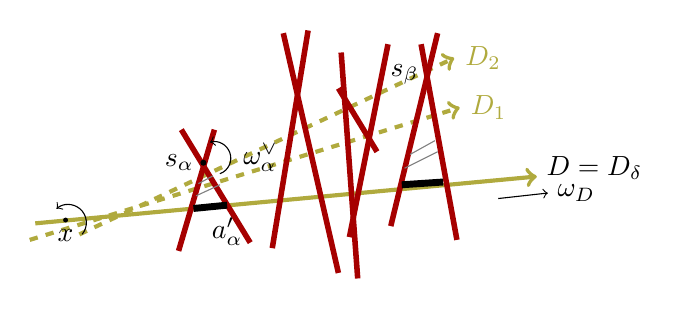
\begin{tikzpicture}[x=.7cm,y=.7cm]
\draw[yellow!65!black,line width=1.5pt,->] (0,.8)--(9.1,1.65);
\node[right] at (9.1,1.8) {$D=D_{\unsure{\delta}}$};
\draw[->] (8.4,1.25)--(9.3,1.35) node[right] {$\omega_D$};
\draw[yellow!65!black,line width=1.5pt,dashed,->] (-.1,.5)--(7.7,2.9) node[right] {$D_1$};
\draw[yellow!65!black,line width=1.5pt,dashed,->] (.8,.6)--(7.6,3.8) node[right] {$D_2$};
\draw[red!65!black,line width=2pt] (2.6,.3)--(3.25,2.5);
\draw[red!65!black,line width=2pt] (2.65,2.5)--(3.9,.45);
\draw[red!65!black,line width=2pt] (4.3,.35)--(4.95,4.3);
\draw[red!65!black,line width=2pt] (4.5,4.25)--(5.5,-.1);
\draw[red!65!black,line width=2pt] (5.55,3.9)--(5.85,-.2);
\draw[red!65!black,line width=2pt] (5.7,.55)--(6.4,4.05);
\draw[red!65!black,line width=2pt] (5.5,3.25)--(6.2,2.1);
\draw[red!65!black,line width=2pt] (6.45,.75)--(7.3,4.25);
\draw[red!65!black,line width=2pt] (7,4.05)--(7.65,.5);
\draw[line width=2.5pt] (2.87,1.07)--(3.48,1.13) node[below] {$a'_\alpha$};
\draw[line width=2.5pt] (6.65,1.5)--(7.4,1.55);
\draw[gray] (2.92,1.3)--(3.35,1.5);
\draw[gray] (2.96,1.52)--(3.22,1.66);
\draw[gray] (6.7,1.8)--(7.3,2.1);
\draw[gray] (6.8,2.05)--(7.25,2.3);
\fill (3.05,1.9) circle (.055) node[left] {$s_\alpha$};
\node[left] at (7.13,3.5) {$s_\beta$};
\fill (.55,.86) circle (.045) node[below] {$x$};
\draw[->] (.85,.6) arc[start angle=-40,end angle=130,radius=.33];
\draw[->] (3.35,1.7) arc[start angle=-70,end angle=105,radius=.3];
\node[right] at (3.6,2) {$\omega_\alpha^\vee$};
\end{tikzpicture}}

Partons avec une orientation $\omega_F$ de
$F$ ($\mapsto\omega_D$ de $D$) et une
arête $a_\alpha$ ($\mapsto s_\alpha$ sommet de $\Sigma$)
allant de $\delta_0\in F$ ($\mapsto D=D_{\delta_0}$) en
ligne droite vers un pt $\delta_1$ voisin de
$a_\alpha$ --- i.e. \unsure{faisons} \unsure{choisissons}
un pt $x$ sur $D$ et une orientation
de rotation en $x$, et faisons pivoter
\margin{78}
\scanpage{80}
$D=D_0=D_{\delta_0}$ autour de $x$ dans le sens de
l'orientation donnée, jusqu'en $D_1$ passant
par $s_\alpha$ (cette opération est anodine,
on aurait pu commencer par un point
$\delta_1$ voisin de $a_\alpha$). Puis suivant le long de
$a_\alpha$ suivant l'orientation induite par $F$
--- ce qui signifie que $D_1$ pivote autour de
$s_\alpha$, dans un sens qu'il faudra expliciter
tantôt (déterminé par l'orientation de $D_1$ déduite
de celle de $D_0$ par trans. pal., et la rive
privilégiée dont on dispose. Notons que l'
orientation \inserted{$\omega_\alpha$} de $\Delta_\alpha$ qui porte $a_\alpha$, celle $\unsure{\omega_{\delta_1}}$ du point
$\delta_1$ sur $\Delta_\alpha$, et la rive $\rho_\alpha$ de $\Delta_\alpha$ déterminée
par $F$, forment un syst. compatible au sens de
Stokes, et qu'il s'ensuit que les
orientations correspondantes en l'élément de
contact $(s_\alpha,D_1)$, $\omega=\omega_\alpha^\vee\in\uline{\omega}(X,s_\alpha)$, $\omega_{\delta_1}^\vee=\omega_{D_1}$, et
$\rho_\alpha^\vee=$ rive de balayage, forment un système
\uline{anticompatible}, i.e. l'orientation $\omega_{D_1}$ de $D_1$
est \uline{opposée} à celle induite par $\omega$ sur la
rive de balayage (cf figure). Ceci peut \unsure{se|ainsi}
se propager le long de $a_\alpha$ \inserted{dans la direction $\omega_\alpha$} ce qui fait tourner
$D_1$ autour de $s_\alpha$ dans la \unsure{direction},
indiquée, jusqu'au moment où
on heurte un premier sommet
\inserted{(qui sera $s_\beta$)} --- qui est aussi celui où le
point mobile $\delta$ sur $a_\alpha$ arrive
au sommet $\delta_2$, rencontre de
\deleted{$\unsure{\Delta_\alpha\text{ et}}$} $a_\alpha$ et $a_\beta$ i.e. de $\Delta_\alpha$ et $\Delta_\beta$
[Bien sûr, \inserted{entre les arcs de} \deleted{\unsure{en cours du}}
\deleted{déplacement de $D_1$, \unsure{arêtes}}
spécialisations correspondantes $a'_\alpha$ et
$a'_\beta$, il peut y avoir, dans un
sens comme dans l'autre
($\omega_D$ ou l'orientation opposée) bien
d'autres arcs de spécialisation, mais
correspondants à des sommets $s_\gamma$
qui ne sont pas atteints au cours
du balayage]. A partir de $s_\beta,D_\beta$
on continue comme précédemment.
\margin{79}
\scanpage{81}
\figure{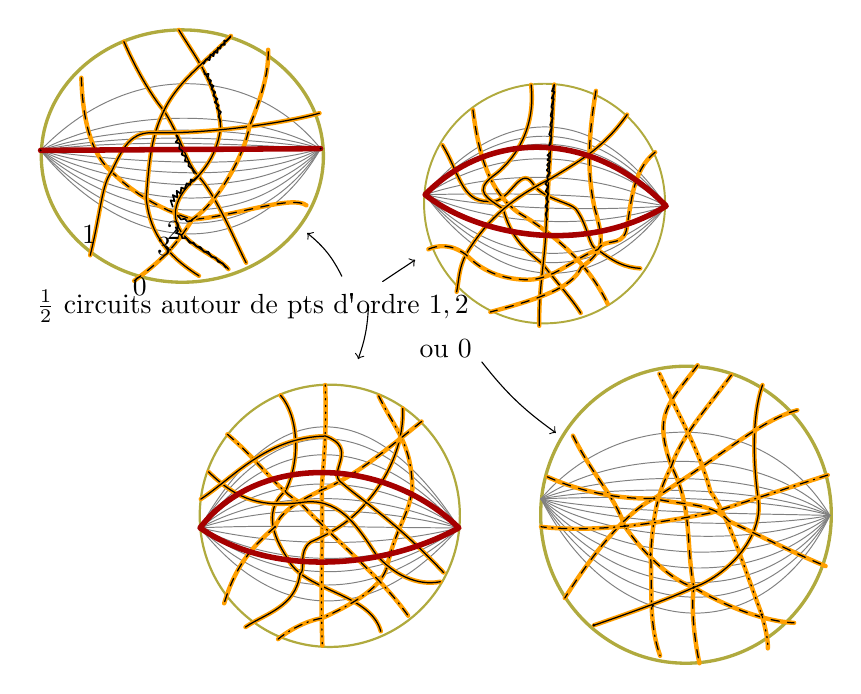
\begin{tikzpicture}[x=.0045cm,y=-.0045cm,line cap=round,line join=round]
\draw[yellow!65!black,line width=1.2pt] (650,451) ellipse (398 and 356);
\draw[gray,line width=.35pt] (250,435) .. controls (500,175) and (850,195) .. (1040,430);
\draw[gray,line width=.35pt] (250,435) .. controls (500,305) and (850,325) .. (1040,430);
\draw[gray,line width=.35pt] (250,435) .. controls (500,350) and (850,370) .. (1040,430);
\draw[gray,line width=.35pt] (250,435) .. controls (500,380) and (850,400) .. (1040,430);
\draw[gray,line width=.35pt] (250,435) .. controls (500,400) and (850,420) .. (1040,430);
\draw[gray,line width=.35pt] (250,435) .. controls (500,470) and (850,490) .. (1040,430);
\draw[gray,line width=.35pt] (250,435) .. controls (500,510) and (850,530) .. (1040,430);
\draw[gray,line width=.35pt] (250,435) .. controls (500,555) and (850,575) .. (1040,430);
\draw[gray,line width=.35pt] (250,435) .. controls (500,605) and (850,625) .. (1040,430);
\draw[gray,line width=.35pt] (250,435) .. controls (500,650) and (850,670) .. (1040,430);
\draw[gray,line width=.35pt] (250,435) .. controls (500,700) and (850,720) .. (1040,430);
\draw[gray,line width=.35pt] (250,435) .. controls (500,740) and (850,760) .. (1040,430);
\draw[orange!75!yellow,line width=1.6pt] (365,230) .. controls (370,390) and (410,460) .. (450,495) .. controls (520,565) and (610,610) .. (680,630) .. controls (800,620) and (960,560) .. (1000,590);
\draw[black,line width=.45pt,dashed] (365,230) .. controls (370,390) and (410,460) .. (450,495) .. controls (520,565) and (610,610) .. (680,630) .. controls (800,620) and (960,560) .. (1000,590);
\draw[orange!75!yellow,line width=1.6pt] (485,128) .. controls (525,220) and (570,290) .. (598,323) .. controls (650,405) and (660,470) .. (695,507) .. controls (750,570) and (795,684) .. (830,752);
\draw[black,line width=.45pt] (485,128) .. controls (525,220) and (570,290) .. (598,323) .. controls (650,405) and (660,470) .. (695,507) .. controls (750,570) and (795,684) .. (830,752);
\draw[orange!75!yellow,line width=1.6pt] (640,95) .. controls (690,178) and (748,245) .. (758,370) .. controls (750,438) and (720,478) .. (695,507) .. controls (641,552) and (608,610) .. (648,667) .. controls (680,711) and (750,735) .. (780,770);
\draw[black,line width=.45pt] (640,95) .. controls (690,178) and (748,245) .. (758,370) .. controls (750,438) and (720,478) .. (695,507) .. controls (641,552) and (608,610) .. (648,667) .. controls (680,711) and (750,735) .. (780,770);
\draw[orange!75!yellow,line width=1.6pt] (787,112) .. controls (720,183) and (640,235) .. (598,323) .. controls (560,400) and (556,474) .. (548,569) .. controls (556,651) and (590,722) .. (697,789);
\draw[black,line width=.45pt] (787,112) .. controls (720,183) and (640,235) .. (598,323) .. controls (560,400) and (556,474) .. (548,569) .. controls (556,651) and (590,722) .. (697,789);
\draw[orange!75!yellow,line width=1.6pt] (390,731) .. controls (421,605) and (422,533) .. (450,495) .. controls (485,420) and (506,388) .. (558,385) .. controls (707,390) and (932,360) .. (1037,330);
\draw[black,line width=.45pt] (390,731) .. controls (421,605) and (422,533) .. (450,495) .. controls (485,420) and (506,388) .. (558,385) .. controls (707,390) and (932,360) .. (1037,330);
\draw[orange!75!yellow,line width=1.6pt] (514,803) .. controls (590,747) and (631,706) .. (678,630) .. controls (753,580) and (827,443) .. (839,368) .. controls (879,270) and (894,209) .. (892,151);
\draw[black,line width=.45pt,dashed] (514,803) .. controls (590,747) and (631,706) .. (678,630) .. controls (753,580) and (827,443) .. (839,368) .. controls (879,270) and (894,209) .. (892,151);
\draw[red!65!black,line width=2pt] (250,435)--(1040,430);
\fill (250,435) circle (3);
\fill (1040,430) circle (3);
\fill (450,495) circle (3);
\fill (598,323) circle (3);
\fill (695,507) circle (3);
\fill (678,630) circle (3);
\fill (616,715) circle (3);
\node at (530,818) {$0$};
\node at (387,673) {$\unsure{1}$};
\node at (626,660) {$\unsure{2}$};
\node at (598,707) {$\unsure{3}$};
\draw[yellow!65!black,line width=.7pt] (1672,585) ellipse (340 and 338);
\draw[gray,line width=.35pt] (1335,560) .. controls (1550,300) and (1820,300) .. (2015,592);
\draw[gray,line width=.35pt] (1335,560) .. controls (1550,335) and (1820,335) .. (2015,592);
\draw[gray,line width=.35pt] (1335,560) .. controls (1550,365) and (1820,365) .. (2015,592);
\draw[gray,line width=.35pt] (1335,560) .. controls (1550,420) and (1820,420) .. (2015,592);
\draw[gray,line width=.35pt] (1335,560) .. controls (1550,490) and (1820,490) .. (2015,592);
\draw[gray,line width=.35pt] (1335,560) .. controls (1550,555) and (1820,555) .. (2015,592);
\draw[gray,line width=.35pt] (1335,560) .. controls (1550,605) and (1820,605) .. (2015,592);
\draw[gray,line width=.35pt] (1335,560) .. controls (1550,655) and (1820,655) .. (2015,592);
\draw[gray,line width=.35pt] (1335,560) .. controls (1550,715) and (1820,715) .. (2015,592);
\draw[gray,line width=.35pt] (1335,560) .. controls (1550,775) and (1820,775) .. (2015,592);
\draw[gray,line width=.35pt] (1335,560) .. controls (1550,810) and (1820,810) .. (2015,592);
\draw[gray,line width=.35pt] (1335,560) .. controls (1550,850) and (1820,850) .. (2015,592);
\draw[orange!75!yellow,line width=1.6pt] (1384,420) .. controls (1430,495) and (1438,580) .. (1512,579) .. controls (1572,593) and (1601,474) .. (1638,527) .. controls (1665,572) and (1740,580) .. (1760,600) .. controls (1800,655) and (1795,710) .. (1822,715) .. controls (1870,752) and (1900,765) .. (1942,768);
\draw[black,line width=.45pt] (1384,420) .. controls (1430,495) and (1438,580) .. (1512,579) .. controls (1572,593) and (1601,474) .. (1638,527) .. controls (1665,572) and (1740,580) .. (1760,600) .. controls (1800,655) and (1795,710) .. (1822,715) .. controls (1870,752) and (1900,765) .. (1942,768);
\draw[orange!75!yellow,line width=1.6pt] (1470,321) .. controls (1490,488) and (1535,564) .. (1597,610) .. controls (1680,660) and (1790,742) .. (1850,868);
\draw[black,line width=.45pt,dashed] (1470,321) .. controls (1490,488) and (1535,564) .. (1597,610) .. controls (1680,660) and (1790,742) .. (1850,868);
\draw[orange!75!yellow,line width=1.6pt] (1634,250) .. controls (1650,390) and (1570,477) .. (1527,507) .. controls (1470,551) and (1510,569) .. (1555,600) .. controls (1578,682) and (1615,714) .. (1665,754) .. controls (1710,812) and (1750,855) .. (1774,894);
\draw[black,line width=.45pt] (1634,250) .. controls (1650,390) and (1570,477) .. (1527,507) .. controls (1470,551) and (1510,569) .. (1555,600) .. controls (1578,682) and (1615,714) .. (1665,754) .. controls (1710,812) and (1750,855) .. (1774,894);
\draw[orange!75!yellow,line width=1.6pt] (1699,249) .. controls (1692,400) and (1680,553) .. (1676,659) .. controls (1672,751) and (1655,828) .. (1657,930);
\draw[black,line width=.45pt] (1699,249) .. controls (1692,400) and (1680,553) .. (1676,659) .. controls (1672,751) and (1655,828) .. (1657,930);
\draw[orange!75!yellow,line width=1.6pt] (1817,267) .. controls (1791,420) and (1795,511) .. (1813,597) .. controls (1840,694) and (1842,716) .. (1775,766) .. controls (1748,827) and (1640,858) .. (1519,891);
\draw[black,line width=.45pt,dashed] (1817,267) .. controls (1791,420) and (1795,511) .. (1813,597) .. controls (1840,694) and (1842,716) .. (1775,766) .. controls (1748,827) and (1640,858) .. (1519,891);
\draw[orange!75!yellow,line width=1.6pt] (1905,334) .. controls (1840,425) and (1784,457) .. (1692,513) .. controls (1590,565) and (1514,621) .. (1450,729) .. controls (1430,766) and (1430,804) .. (1424,834);
\draw[black,line width=.45pt] (1905,334) .. controls (1840,425) and (1784,457) .. (1692,513) .. controls (1590,565) and (1514,621) .. (1450,729) .. controls (1430,766) and (1430,804) .. (1424,834);
\draw[orange!75!yellow,line width=1.6pt] (1984,440) .. controls (1917,495) and (1918,584) .. (1902,663) .. controls (1888,709) and (1840,681) .. (1822,715) .. controls (1755,739) and (1700,799) .. (1625,800) .. controls (1530,799) and (1480,759) .. (1450,729) .. controls (1407,697) and (1368,703) .. (1344,714);
\draw[black,line width=.45pt,dashed] (1984,440) .. controls (1917,495) and (1918,584) .. (1902,663) .. controls (1888,709) and (1840,681) .. (1822,715) .. controls (1755,739) and (1700,799) .. (1625,800) .. controls (1530,799) and (1480,759) .. (1450,729) .. controls (1407,697) and (1368,703) .. (1344,714);
\draw[red!65!black,line width=2pt] (1335,560) .. controls (1500,390) and (1790,362) .. (2015,592) .. controls (1780,735) and (1480,674) .. cycle;
\draw[yellow!65!black,line width=.8pt] (1066,1466) ellipse (367 and 370);
\draw[gray,line width=.35pt] (700,1500) .. controls (915,1115) and (1188,1125) .. (1430,1500);
\draw[gray,line width=.35pt] (700,1500) .. controls (915,1160) and (1188,1170) .. (1430,1500);
\draw[gray,line width=.35pt] (700,1500) .. controls (915,1220) and (1188,1230) .. (1430,1500);
\draw[gray,line width=.35pt] (700,1500) .. controls (915,1280) and (1188,1290) .. (1430,1500);
\draw[gray,line width=.35pt] (700,1500) .. controls (915,1330) and (1188,1340) .. (1430,1500);
\draw[gray,line width=.35pt] (700,1500) .. controls (915,1385) and (1188,1395) .. (1430,1500);
\draw[gray,line width=.35pt] (700,1500) .. controls (915,1430) and (1188,1440) .. (1430,1500);
\draw[gray,line width=.35pt] (700,1500) .. controls (915,1490) and (1188,1500) .. (1430,1500);
\draw[gray,line width=.35pt] (700,1500) .. controls (915,1550) and (1188,1560) .. (1430,1500);
\draw[gray,line width=.35pt] (700,1500) .. controls (915,1610) and (1188,1620) .. (1430,1500);
\draw[gray,line width=.35pt] (700,1500) .. controls (915,1660) and (1188,1670) .. (1430,1500);
\draw[gray,line width=.35pt] (700,1500) .. controls (915,1710) and (1188,1720) .. (1430,1500);
\draw[gray,line width=.35pt] (700,1500) .. controls (915,1770) and (1188,1780) .. (1430,1500);
\draw[orange!75!yellow,line width=1.6pt] (927,1126) .. controls (976,1182) and (986,1304) .. (941,1396) .. controls (883,1445) and (899,1516) .. (948,1588) .. controls (990,1678) and (1180,1683) .. (1210,1792);
\draw[black,line width=.45pt] (927,1126) .. controls (976,1182) and (986,1304) .. (941,1396) .. controls (883,1445) and (899,1516) .. (948,1588) .. controls (990,1678) and (1180,1683) .. (1210,1792);
\draw[orange!75!yellow,line width=1.6pt] (1053,1097) .. controls (1059,1250) and (1044,1355) .. (1043,1393) .. controls (1048,1511) and (1039,1674) .. (1045,1832);
\draw[black,line width=.45pt,dotted] (1053,1097) .. controls (1059,1250) and (1044,1355) .. (1043,1393) .. controls (1048,1511) and (1039,1674) .. (1045,1832);
\draw[orange!75!yellow,line width=1.6pt] (1204,1128) .. controls (1250,1223) and (1297,1260) .. (1299,1391) .. controls (1287,1471) and (1254,1494) .. (1226,1615) .. controls (1206,1675) and (1118,1721) .. (1044,1755) .. controls (997,1762) and (945,1793) .. (920,1814);
\draw[black,line width=.45pt,dash dot] (1204,1128) .. controls (1250,1223) and (1297,1260) .. (1299,1391) .. controls (1287,1471) and (1254,1494) .. (1226,1615) .. controls (1206,1675) and (1118,1721) .. (1044,1755) .. controls (997,1762) and (945,1793) .. (920,1814);
\draw[orange!75!yellow,line width=1.6pt] (1272,1163) .. controls (1275,1263) and (1231,1359) .. (1168,1430) .. controls (1115,1494) and (1049,1523) .. (1012,1540) .. controls (974,1567) and (1000,1620) .. (982,1630) .. controls (969,1725) and (881,1743) .. (828,1780);
\draw[black,line width=.45pt] (1272,1163) .. controls (1275,1263) and (1231,1359) .. (1168,1430) .. controls (1115,1494) and (1049,1523) .. (1012,1540) .. controls (974,1567) and (1000,1620) .. (982,1630) .. controls (969,1725) and (881,1743) .. (828,1780);
\draw[orange!75!yellow,line width=1.6pt] (1325,1200) .. controls (1225,1280) and (1130,1360) .. (1043,1393) .. controls (995,1418) and (930,1446) .. (912,1497) .. controls (841,1558) and (798,1613) .. (768,1713);
\draw[black,line width=.45pt,dashed] (1325,1200) .. controls (1225,1280) and (1130,1360) .. (1043,1393) .. controls (995,1418) and (930,1446) .. (912,1497) .. controls (841,1558) and (798,1613) .. (768,1713);
\draw[orange!75!yellow,line width=1.6pt] (777,1236) .. controls (867,1312) and (920,1394) .. (982,1429) .. controls (1088,1540) and (1212,1641) .. (1287,1748);
\draw[black,line width=.45pt,dash dot] (777,1236) .. controls (867,1312) and (920,1394) .. (982,1429) .. controls (1088,1540) and (1212,1641) .. (1287,1748);
\draw[orange!75!yellow,line width=1.6pt] (724,1342) .. controls (810,1427) and (879,1440) .. (982,1429) .. controls (1090,1411) and (1140,1490) .. (1197,1576) .. controls (1247,1632) and (1312,1665) .. (1378,1652);
\draw[black,line width=.45pt] (724,1342) .. controls (810,1427) and (879,1440) .. (982,1429) .. controls (1090,1411) and (1140,1490) .. (1197,1576) .. controls (1247,1632) and (1312,1665) .. (1378,1652);
\draw[orange!75!yellow,line width=1.6pt] (702,1419) .. controls (795,1358) and (886,1245) .. (1054,1241) .. controls (1145,1275) and (1066,1335) .. (1093,1367) .. controls (1155,1423) and (1248,1478) .. (1387,1626);
\draw[black,line width=.45pt] (702,1419) .. controls (795,1358) and (886,1245) .. (1054,1241) .. controls (1145,1275) and (1066,1335) .. (1093,1367) .. controls (1155,1423) and (1248,1478) .. (1387,1626);
\draw[red!65!black,line width=2pt] (700,1500) .. controls (864,1285) and (1225,1299) .. (1430,1500) .. controls (1212,1619) and (898,1638) .. cycle;
\fill (941,1396) circle (3);
\fill (1043,1393) circle (3);
\fill (982,1429) circle (3);
\fill (912,1497) circle (3);
\fill (1168,1430) circle (3);
\fill (982,1630) circle (3);
\fill (1226,1615) circle (3);
\draw[yellow!65!black,line width=1.2pt] (2071,1463) ellipse (410 and 419);
\draw[gray,line width=.35pt] (1662,1418) .. controls (1880,1160) and (2295,1160) .. (2477,1465);
\draw[gray,line width=.35pt] (1662,1418) .. controls (1880,1270) and (2295,1270) .. (2477,1465);
\draw[gray,line width=.35pt] (1662,1418) .. controls (1880,1335) and (2295,1335) .. (2477,1465);
\draw[gray,line width=.35pt] (1662,1418) .. controls (1880,1380) and (2295,1380) .. (2477,1465);
\draw[gray,line width=.35pt] (1662,1418) .. controls (1880,1410) and (2295,1410) .. (2477,1465);
\draw[gray,line width=.35pt] (1662,1418) .. controls (1880,1460) and (2295,1460) .. (2477,1465);
\draw[gray,line width=.35pt] (1662,1418) .. controls (1880,1500) and (2295,1500) .. (2477,1465);
\draw[gray,line width=.35pt] (1662,1418) .. controls (1880,1550) and (2295,1550) .. (2477,1465);
\draw[gray,line width=.35pt] (1662,1418) .. controls (1880,1610) and (2295,1610) .. (2477,1465);
\draw[gray,line width=.35pt] (1662,1418) .. controls (1880,1670) and (2295,1670) .. (2477,1465);
\draw[gray,line width=.35pt] (1662,1418) .. controls (1880,1725) and (2295,1725) .. (2477,1465);
\draw[gray,line width=.35pt] (1662,1418) .. controls (1880,1780) and (2295,1780) .. (2477,1465);
\draw[gray,line width=.35pt] (1662,1418) .. controls (1880,1840) and (2295,1840) .. (2477,1465);
\draw[orange!75!yellow,line width=1.6pt] (1752,1240) .. controls (1810,1357) and (1867,1405) .. (1898,1495) .. controls (1937,1553) and (2017,1643) .. (2093,1668) .. controls (2180,1720) and (2289,1764) .. (2376,1768);
\draw[black,line width=.45pt,dashed] (1752,1240) .. controls (1810,1357) and (1867,1405) .. (1898,1495) .. controls (1937,1553) and (2017,1643) .. (2093,1668) .. controls (2180,1720) and (2289,1764) .. (2376,1768);
\draw[orange!75!yellow,line width=1.6pt] (1996,1065) .. controls (2058,1199) and (2110,1284) .. (2140,1398) .. controls (2190,1464) and (2235,1612) .. (2285,1745) .. controls (2294,1780) and (2303,1815) .. (2302,1840);
\draw[black,line width=.45pt,dotted] (1996,1065) .. controls (2058,1199) and (2110,1284) .. (2140,1398) .. controls (2190,1464) and (2235,1612) .. (2285,1745) .. controls (2294,1780) and (2303,1815) .. (2302,1840);
\draw[orange!75!yellow,line width=1.6pt] (2104,1041) .. controls (2024,1149) and (1976,1175) .. (2030,1326) .. controls (2090,1443) and (2070,1545) .. (2093,1668) .. controls (2084,1734) and (2098,1832) .. (2109,1882);
\draw[black,line width=.45pt,dashed] (2104,1041) .. controls (2024,1149) and (1976,1175) .. (2030,1326) .. controls (2090,1443) and (2070,1545) .. (2093,1668) .. controls (2084,1734) and (2098,1832) .. (2109,1882);
\draw[orange!75!yellow,line width=1.6pt] (2199,1069) .. controls (2138,1153) and (2058,1240) .. (2030,1326) .. controls (1987,1410) and (1980,1463) .. (1971,1576) .. controls (1977,1671) and (1964,1764) .. (1998,1861);
\draw[black,line width=.45pt,dash dot] (2199,1069) .. controls (2138,1153) and (2058,1240) .. (2030,1326) .. controls (1987,1410) and (1980,1463) .. (1971,1576) .. controls (1977,1671) and (1964,1764) .. (1998,1861);
\draw[orange!75!yellow,line width=1.6pt] (2287,1097) .. controls (2255,1190) and (2261,1323) .. (2275,1420) .. controls (2290,1531) and (2180,1638) .. (2093,1668) .. controls (2021,1701) and (1930,1734) .. (1811,1775);
\draw[black,line width=.45pt] (2287,1097) .. controls (2255,1190) and (2261,1323) .. (2275,1420) .. controls (2290,1531) and (2180,1638) .. (2093,1668) .. controls (2021,1701) and (1930,1734) .. (1811,1775);
\draw[orange!75!yellow,line width=1.6pt] (2385,1168) .. controls (2280,1197) and (2182,1290) .. (1981,1417) .. controls (1907,1453) and (1817,1559) .. (1729,1698);
\draw[black,line width=.45pt,dashed] (2385,1168) .. controls (2280,1197) and (2182,1290) .. (1981,1417) .. controls (1907,1453) and (1817,1559) .. (1729,1698);
\draw[orange!75!yellow,line width=1.6pt] (2471,1351) .. controls (2335,1395) and (2231,1430) .. (2140,1458) .. controls (2036,1478) and (1830,1517) .. (1662,1497);
\draw[black,line width=.45pt,dash dot] (2471,1351) .. controls (2335,1395) and (2231,1430) .. (2140,1458) .. controls (2036,1478) and (1830,1517) .. (1662,1497);
\draw[orange!75!yellow,line width=1.6pt] (1680,1356) .. controls (1770,1397) and (1880,1420) .. (1981,1417) .. controls (2060,1438) and (2140,1425) .. (2192,1481) .. controls (2275,1520) and (2382,1574) .. (2465,1608);
\draw[black,line width=.45pt,dashed] (1680,1356) .. controls (1770,1397) and (1880,1420) .. (1981,1417) .. controls (2060,1438) and (2140,1425) .. (2192,1481) .. controls (2275,1520) and (2382,1574) .. (2465,1608);
\fill (1898,1495) circle (4);
\fill (1971,1576) circle (4);
\fill (1981,1417) circle (4);
\fill (2093,1668) circle (4);
\fill (1977,1720) circle (4);
\fill (2285,1745) circle (4);
\fill (1811,1775) circle (4);
\draw[black,line width=.6pt] (786,115)--(774,127)--(768,125)--(770,137)--(760,137)--(757,148)--(750,146)--(749,160)--(740,156)--(738,169)--(729,165)--(727,180)--(717,178)--(710,191);
\draw[black,line width=.6pt] (710,210)--(714,221)--(724,219)--(721,233)--(731,238)--(727,247)--(738,253)--(732,262)--(743,271)--(737,280)--(749,290)--(741,299)--(753,308)--(747,316)--(759,327)--(752,338)--(758,355);
\draw[black,line width=.6pt] (633,392)--(638,403)--(631,412)--(643,416)--(641,430)--(651,437)--(648,447)--(660,452)--(657,465)--(669,468)--(667,479)--(678,486)--(683,499);
\draw[black,line width=.6pt] (693,510)--(682,521)--(674,517)--(672,532)--(662,528)--(657,544)--(647,540)--(645,557)--(634,549)--(636,567)--(623,561)--(628,578)--(617,576)--(623,594);
\draw[black,line width=.6pt] (637,619)--(646,630)--(657,628)--(664,636)--(677,633) (631,652)--(638,663)--(632,668)--(647,673)--(650,683)--(661,682)--(671,696)--(681,695)--(690,706)--(701,708)--(711,721)--(723,721)--(732,735)--(744,738)--(751,749)--(764,754)--(773,766);
\draw[black,line width=.6pt] (1699,252)--(1693,268)--(1700,270)--(1692,288)--(1698,290)--(1691,312)--(1695,318)--(1689,337)--(1695,344)--(1688,363)--(1692,371)--(1685,390)--(1692,398)--(1685,421);
\draw[black,line width=.6pt] (1688,441)--(1680,449)--(1687,453)--(1680,462)--(1688,466)--(1679,476)--(1685,482)--(1678,491)--(1687,498)--(1679,508)--(1682,519)--(1674,530)--(1683,537)--(1675,550)--(1683,557)--(1676,570)--(1682,580)--(1674,593)--(1681,601)--(1675,614)--(1679,631);
\node[anchor=west] at (212,875) {$\frac12$ circuits autour de pts d\textquotesingle ordre $1,2$};
\draw[->] (1100,790) to[bend right=12] (1002,668);
\draw[->] (1215,805)--(1307,744);
\draw[->] (1175,878) to[bend left=8] (1146,1024);
\node at (1393,994) {ou $0$};
\draw[->] (1495,1032) to[bend right=8] (1704,1232);
\end{tikzpicture}} % crop-candidate: scan 81
\margin{80}
\scanpage{82}
\margin{81}
\texttt{D A T A S E T S\quad P I C T U R E S}
\begin{verbatim}
******************************************************************************************************************
*              *                  *        *       *             *            *     *       *        *           *
*   DDNAME     * DESTINATION      * CLASS  *COPIES *  RECORDS-NB *  BYTES-NB  *FORM * FCB   * UCS    *SPIN HOLD  *
*              *                  *        *       *             *            *     *       *        *           *
******************************************************************************************************************
*              *                  *        *       *             *            *     *       *        *           *
*    SYSOS3    * CNU     M06      *    A   *   1   *         67  *      3,893 *STD. * ****  * ****   *           *
******************************************************************************************************************
\end{verbatim}

\deleted{\diagram{\begin{array}{ccc@{\qquad}ccc@{\qquad}ccc}
\chi_0&\chi_1&\chi_2&&&&&&\\
1&\bar\epsilon&0&1&1&0&1&1&0\\
1&\unsure{\xi}&0&1&\unsure{\xi}&0&1&\unsure{0|\xi}&\unsure{0}\\
1&\unsure{\eta}&1&1&\unsure{\eta}&1&1&\unsure{\eta}&\unsure{1}\\
&\unsure{\xi}-1&&&&&1-\unsure{\bar\epsilon}=1&&
\end{array}}}

\deleted{\diagram{\begin{array}{ll}
\left.\begin{array}{ll}\chi_0&\text{orientation de }D\\
\chi_1&\text{sens des }(n\text{-gones}\ \inserted{\text{duaux}}\text{ inscrits})\end{array}\right\}
&\begin{array}{l}\text{caractères fondamentaux}\\\text{sur }\unsure{\mathbb D_2}\end{array}\\
\chi_2&\text{caractère parité}
\end{array}}}

\deleted{\uline{NB} le caractère d'orientation pour
$\unsure{\mathcal X}$ est $\chi_0\chi_2$,
le caractère ``\unsure{longueurs circuits}''
est $\chi_0\chi_1$}

\deleted{\[\epsilon=\text{parité de }n\in\{0,1\}\qquad
\bar\epsilon=\text{opposé de }\epsilon=\epsilon-1\bmod2\]}

\deleted{\diagram{\begin{array}{lccc}
&\chi_0&\chi_1&\chi_2\\
\begin{array}{l}\frac12\text{ tour }\deleted{\unsure{autour}}\text{ d'un trou}\\
(\text{en }2n+\uuline{2}\text{ pas})\end{array}
&1&\unsure{\bar\epsilon}\deleted{\unsure{1}}&0\\
\begin{array}{l}\frac12\text{ tour autour}\\\deleted{\unsure{d'un sommet}}\\\deleted{\unsure{d'un point}}\\\text{d'ordre }\alpha\end{array}
&1&?&\alpha
\end{array}}}

\deleted{$\ell$ lacet en $F$}

\deleted{\deleted{$\unsure{\beta}$} $\unsure{u}(\ell)$ : Autom de $\operatorname{Pol}_0(F)$ (polygone de degré $2n$)}
\deleted{\[\chi_0(\ell)\mathrel{\mathop=^{\mathrm{def}}}\unsure{\operatorname{sgn}}\,\unsure{u}(\ell)=\left\{\vphantom{\frac11}\right.\]}
\deleted{\deleted{\unsure{si de}}}

\deleted{\deleted{1) Si $\alpha$ pair alors $\chi_0$ et}}

\deleted{Prenant $\alpha$ \deleted{pair} \inserted{impair}, on voit que
\uline{$\chi_0,\chi_2$ indépendants} / et $\chi_1,\chi_2$ aussi si $n$
pair, i.e. $\bar\epsilon=1$
\[\text{i.e. }\chi_0,\unsure{\chi_2|\chi}\text{ indépendants}\]}

\deleted{\uline{$\chi_0$}\qquad \uline{$n$ pair}\qquad
$\Pi\longrightarrow\mathbb D_{2n}$ surjectif
\[\text{et : }\Pi\longrightarrow\mathbb D_{2n}\times\{\pm1\}\text{ a une image qui contient }\mathbb D_n\times\{\pm1\}\]}

\deleted{\diagram{\begin{array}{lccc}
\uline{n\text{ pair}}&1&1&0\\
&1&?&\alpha\\[1em]
\uline{n\text{ impair}}&1&0&0\\
&1&?&\alpha
\end{array}}}

\deleted{$\chi_2$ n'est pas lié à $\chi_0$, ni à $\chi_2$ --- il est possible que
$\chi_2,\chi_1$ le soient, d'où tjrs $?=1$}
\deleted{\margin{$\chi_0$}}
\figure{\begin{tikzpicture}[x=.006cm,y=-.006cm]
\draw (0,100)--(1000,1800);
\draw (600,0)--(1800,1700);
\draw (-500,700)--(1700,1900);
\draw (650,1850)--(650,2050);
\draw (650,1850)--(1700,1820) .. controls (1830,1810) and (1790,1740) .. (1840,1730)--(2300,1730);
\end{tikzpicture}}
\scanpage{83}
\figure{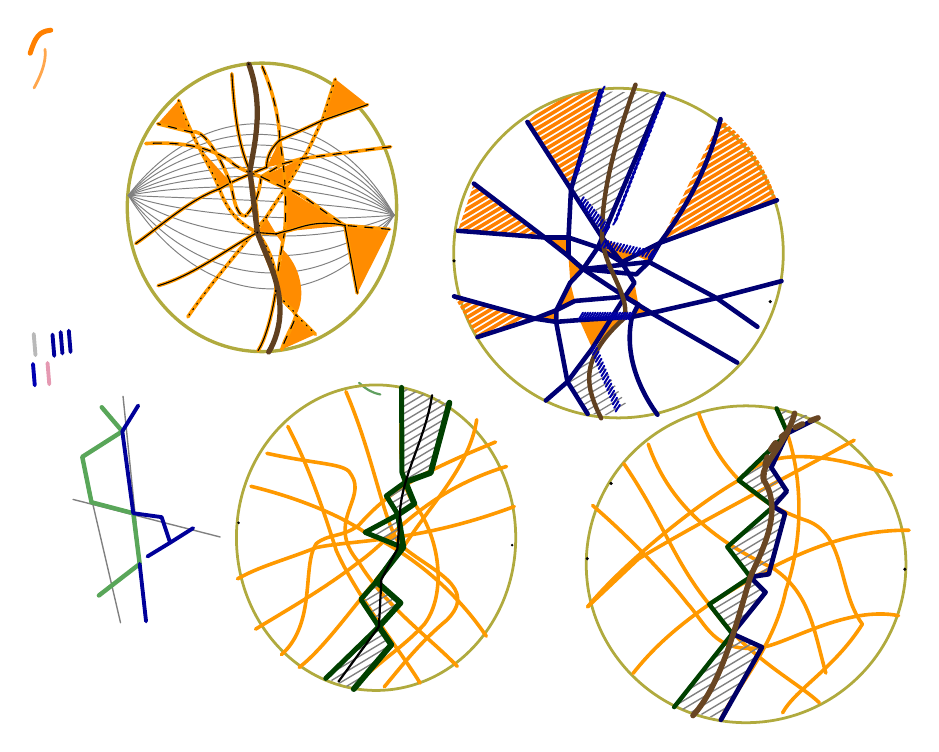
\begin{tikzpicture}[x=.0045cm,y=-.0045cm,line cap=round,line join=round]
\draw[orange,line width=1.8pt] (90,137) .. controls (105,90) and (115,76) .. (148,72);
\draw[orange!70,line width=1pt] (132,126) .. controls (137,166) and (114,211) .. (101,235);
\draw[gray!55,line width=1.4pt] (100,929)--(105,989);
\draw[blue!60!black,line width=1.4pt] (153,931)--(158,991);
\draw[blue!60!black,line width=1.4pt] (176,924)--(181,984);
\draw[blue!60!black,line width=1.4pt] (199,920)--(204,980);
\draw[blue!70!black,line width=1.4pt] (98,1014)--(103,1074);
\draw[purple!40,line width=1.4pt] (139,1011)--(144,1071);
\draw[yellow!65!black,line width=1.2pt] (744,572) ellipse (380 and 407);
\draw[gray,line width=.35pt] (367,538) .. controls (580,260) and (930,260) .. (1117,594);
\draw[gray,line width=.35pt] (367,538) .. controls (580,300) and (930,300) .. (1117,594);
\draw[gray,line width=.35pt] (367,538) .. controls (580,340) and (930,340) .. (1117,594);
\draw[gray,line width=.35pt] (367,538) .. controls (580,385) and (930,385) .. (1117,594);
\draw[gray,line width=.35pt] (367,538) .. controls (580,425) and (930,425) .. (1117,594);
\draw[gray,line width=.35pt] (367,538) .. controls (580,460) and (930,460) .. (1117,594);
\draw[gray,line width=.35pt] (367,538) .. controls (580,500) and (930,500) .. (1117,594);
\draw[gray,line width=.35pt] (367,538) .. controls (580,550) and (930,550) .. (1117,594);
\draw[gray,line width=.35pt] (367,538) .. controls (580,610) and (930,610) .. (1117,594);
\draw[gray,line width=.35pt] (367,538) .. controls (580,680) and (930,680) .. (1117,594);
\draw[gray,line width=.35pt] (367,538) .. controls (580,755) and (930,755) .. (1117,594);
\draw[gray,line width=.35pt] (367,538) .. controls (580,820) and (930,820) .. (1117,594);
\draw[gray,line width=.35pt] (367,538) .. controls (580,880) and (930,880) .. (1117,594);
\fill[orange!90!yellow] (450,336)--(509,270)--(546,360)--cycle;
\fill[orange!90!yellow] (914,327)--(951,210)--(1042,282)--cycle;
\fill[orange!90!yellow] (577,414)--(654,500)--(624,520)--cycle;
\fill[orange!90!yellow] (757,459)--(794,383)--(803,449)--cycle;
\fill[orange!90!yellow] (742,486)--(810,518)--(859,434)--cycle;
\fill[orange!90!yellow] (810,518)--(978,623)--(808,640)--cycle;
\fill[orange!90!yellow] (977,623)--(1104,634)--(1013,814)--cycle;
\fill[orange!90!yellow] (733,641)--(756,600)--(784,647)--cycle;
\fill[orange!90!yellow] (783,647)--(812,640)--(803,676)--cycle;
\fill[orange!90!yellow] (804,692) .. controls (850,736) and (872,818) .. (840,876)--(783,808)--cycle;
\fill[orange!90!yellow] (840,876)--(895,930)--(800,973)--cycle;
\draw[orange!80!yellow,line width=1.3pt] (659,195) .. controls (669,355) and (687,415) .. (710,470) .. controls (724,535) and (734,596) .. (731,643) .. controls (759,731) and (791,777) .. (783,808) .. controls (771,885) and (752,947) .. (733,976);
\draw[black,line width=.4pt] (659,195) .. controls (669,355) and (687,415) .. (710,470) .. controls (724,535) and (734,596) .. (731,643) .. controls (759,731) and (791,777) .. (783,808) .. controls (771,885) and (752,947) .. (733,976);
\draw[orange!80!yellow,line width=1.3pt] (745,175) .. controls (778,251) and (794,331) .. (794,383) .. controls (808,460) and (816,558) .. (808,640) .. controls (799,690) and (787,758) .. (783,808) .. controls (815,852) and (838,865) .. (840,876) .. controls (833,906) and (809,940) .. (800,973);
\draw[black,line width=.4pt,dashed] (745,175) .. controls (778,251) and (794,331) .. (794,383) .. controls (808,460) and (816,558) .. (808,640) .. controls (799,690) and (787,758) .. (783,808) .. controls (815,852) and (838,865) .. (840,876) .. controls (833,906) and (809,940) .. (800,973);
\draw[orange!80!yellow,line width=1.3pt] (509,270) .. controls (550,389) and (602,459) .. (624,520) .. controls (646,580) and (675,615) .. (731,643) .. controls (762,682) and (790,746) .. (783,808) .. controls (815,852) and (838,865) .. (840,876)--(895,930);
\draw[black,line width=.4pt,dotted] (509,270) .. controls (550,389) and (602,459) .. (624,520) .. controls (646,580) and (675,615) .. (731,643) .. controls (762,682) and (790,746) .. (783,808) .. controls (815,852) and (838,865) .. (840,876)--(895,930);
\draw[orange!80!yellow,line width=1.3pt] (951,210)--(914,327) .. controls (890,374) and (870,425) .. (859,434) .. controls (831,489) and (780,562) .. (756,600) .. controls (683,690) and (587,802) .. (535,881);
\draw[black,line width=.4pt,dotted] (951,210)--(914,327) .. controls (890,374) and (870,425) .. (859,434) .. controls (831,489) and (780,562) .. (756,600) .. controls (683,690) and (587,802) .. (535,881);
\draw[orange!80!yellow,line width=1.3pt] (1042,282)--(914,327)--(794,383) .. controls (758,415) and (758,445) .. (757,459) .. controls (709,479) and (668,494) .. (624,520) .. controls (542,547) and (442,638) .. (388,674);
\draw[black,line width=.4pt] (1042,282)--(914,327)--(794,383) .. controls (758,415) and (758,445) .. (757,459) .. controls (709,479) and (668,494) .. (624,520) .. controls (542,547) and (442,638) .. (388,674);
\draw[orange!80!yellow,line width=1.3pt] (1107,401)--(859,434)--(803,449)--(742,486) .. controls (733,554) and (716,576) .. (698,596) .. controls (669,600) and (663,531) .. (654,500) .. controls (614,402) and (572,349) .. (546,360)--(450,336);
\draw[black,line width=.4pt,dashed] (1107,401)--(859,434)--(803,449)--(742,486) .. controls (733,554) and (716,576) .. (698,596) .. controls (669,600) and (663,531) .. (654,500) .. controls (614,402) and (572,349) .. (546,360)--(450,336);
\draw[orange!80!yellow,line width=1.3pt] (1104,634)--(978,623) .. controls (898,573) and (860,532) .. (810,518)--(742,486) .. controls (706,472) and (674,462) .. (654,441) .. controls (585,394) and (492,387) .. (416,392);
\draw[black,line width=.4pt,dashed] (1104,634)--(978,623) .. controls (898,573) and (860,532) .. (810,518)--(742,486) .. controls (706,472) and (674,462) .. (654,441) .. controls (585,394) and (492,387) .. (416,392);
\draw[orange!80!yellow,line width=1.3pt] (1013,814)--(978,623) .. controls (890,604) and (845,634) .. (808,640)--(784,647)--(731,643) .. controls (648,687) and (550,765) .. (451,793);
\draw[black,line width=.4pt] (1013,814)--(978,623) .. controls (890,604) and (845,634) .. (808,640)--(784,647)--(731,643) .. controls (648,687) and (550,765) .. (451,793);
\draw[brown!50!black,line width=1.9pt] (707,168) .. controls (751,290) and (723,390) .. (710,470)--(731,643) .. controls (754,707) and (795,777) .. (795,862) .. controls (795,909) and (780,953) .. (763,980);
\fill (707,168) circle (3);
\fill (546,360) circle (3);
\fill (577,414) circle (3);
\fill (624,520) circle (3);
\fill (654,500) circle (3);
\fill (710,470) circle (3);
\fill (757,459) circle (3);
\fill (794,383) circle (3);
\fill (803,449) circle (3);
\fill (859,434) circle (3);
\fill (914,327) circle (3);
\fill (742,486) circle (3);
\fill (810,518) circle (3);
\fill (698,596) circle (3);
\fill (731,643) circle (3);
\fill (756,600) circle (3);
\fill (784,647) circle (3);
\fill (978,623) circle (3);
\fill (783,808) circle (3);
\fill (840,876) circle (3);
\draw[yellow!65!black,line width=1pt] (1750,701) ellipse (465 and 465);
\begin{scope}\clip (1493,331)--(1616,521)--(1699,244) .. controls (1620,246) and (1540,283) .. cycle;
\draw[orange,line width=1.3pt] (1200,200)--(2250,-430.0);
\draw[orange,line width=1.3pt] (1200,218)--(2250,-412.0);
\draw[orange,line width=1.3pt] (1200,236)--(2250,-394.0);
\draw[orange,line width=1.3pt] (1200,254)--(2250,-376.0);
\draw[orange,line width=1.3pt] (1200,272)--(2250,-358.0);
\draw[orange,line width=1.3pt] (1200,290)--(2250,-340.0);
\draw[orange,line width=1.3pt] (1200,308)--(2250,-322.0);
\draw[orange,line width=1.3pt] (1200,326)--(2250,-304.0);
\draw[orange,line width=1.3pt] (1200,344)--(2250,-286.0);
\draw[orange,line width=1.3pt] (1200,362)--(2250,-268.0);
\draw[orange,line width=1.3pt] (1200,380)--(2250,-250.0);
\draw[orange,line width=1.3pt] (1200,398)--(2250,-232.0);
\draw[orange,line width=1.3pt] (1200,416)--(2250,-214.0);
\draw[orange,line width=1.3pt] (1200,434)--(2250,-196.0);
\draw[orange,line width=1.3pt] (1200,452)--(2250,-178.0);
\draw[orange,line width=1.3pt] (1200,470)--(2250,-160.0);
\draw[orange,line width=1.3pt] (1200,488)--(2250,-142.0);
\draw[orange,line width=1.3pt] (1200,506)--(2250,-124.0);
\draw[orange,line width=1.3pt] (1200,524)--(2250,-106.0);
\draw[orange,line width=1.3pt] (1200,542)--(2250,-88.0);
\draw[orange,line width=1.3pt] (1200,560)--(2250,-70.0);
\draw[orange,line width=1.3pt] (1200,578)--(2250,-52.0);
\draw[orange,line width=1.3pt] (1200,596)--(2250,-34.0);
\draw[orange,line width=1.3pt] (1200,614)--(2250,-16.0);
\draw[orange,line width=1.3pt] (1200,632)--(2250,2.0);
\draw[orange,line width=1.3pt] (1200,650)--(2250,20.0);
\draw[orange,line width=1.3pt] (1200,668)--(2250,38.0);
\draw[orange,line width=1.3pt] (1200,686)--(2250,56.0);
\draw[orange,line width=1.3pt] (1200,704)--(2250,74.0);
\draw[orange,line width=1.3pt] (1200,722)--(2250,92.0);
\draw[orange,line width=1.3pt] (1200,740)--(2250,110.0);
\draw[orange,line width=1.3pt] (1200,758)--(2250,128.0);
\draw[orange,line width=1.3pt] (1200,776)--(2250,146.0);
\draw[orange,line width=1.3pt] (1200,794)--(2250,164.0);
\draw[orange,line width=1.3pt] (1200,812)--(2250,182.0);
\draw[orange,line width=1.3pt] (1200,830)--(2250,200.0);
\draw[orange,line width=1.3pt] (1200,848)--(2250,218.0);
\draw[orange,line width=1.3pt] (1200,866)--(2250,236.0);
\draw[orange,line width=1.3pt] (1200,884)--(2250,254.0);
\draw[orange,line width=1.3pt] (1200,902)--(2250,272.0);
\draw[orange,line width=1.3pt] (1200,920)--(2250,290.0);
\draw[orange,line width=1.3pt] (1200,938)--(2250,308.0);
\draw[orange,line width=1.3pt] (1200,956)--(2250,326.0);
\draw[orange,line width=1.3pt] (1200,974)--(2250,344.0);
\draw[orange,line width=1.3pt] (1200,992)--(2250,362.0);
\draw[orange,line width=1.3pt] (1200,1010)--(2250,380.0);
\draw[orange,line width=1.3pt] (1200,1028)--(2250,398.0);
\draw[orange,line width=1.3pt] (1200,1046)--(2250,416.0);
\draw[orange,line width=1.3pt] (1200,1064)--(2250,434.0);
\draw[orange,line width=1.3pt] (1200,1082)--(2250,452.0);
\draw[orange,line width=1.3pt] (1200,1100)--(2250,470.0);
\draw[orange,line width=1.3pt] (1200,1118)--(2250,488.0);
\draw[orange,line width=1.3pt] (1200,1136)--(2250,506.0);
\draw[orange,line width=1.3pt] (1200,1154)--(2250,524.0);
\draw[orange,line width=1.3pt] (1200,1172)--(2250,542.0);
\draw[orange,line width=1.3pt] (1200,1190)--(2250,560.0);
\end{scope}
\begin{scope}\clip (2038,323) .. controls (2125,386) and (2170,475) .. (2197,552)--(1867,672)--cycle;
\draw[orange,line width=1.3pt] (1200,200)--(2250,-430.0);
\draw[orange,line width=1.3pt] (1200,218)--(2250,-412.0);
\draw[orange,line width=1.3pt] (1200,236)--(2250,-394.0);
\draw[orange,line width=1.3pt] (1200,254)--(2250,-376.0);
\draw[orange,line width=1.3pt] (1200,272)--(2250,-358.0);
\draw[orange,line width=1.3pt] (1200,290)--(2250,-340.0);
\draw[orange,line width=1.3pt] (1200,308)--(2250,-322.0);
\draw[orange,line width=1.3pt] (1200,326)--(2250,-304.0);
\draw[orange,line width=1.3pt] (1200,344)--(2250,-286.0);
\draw[orange,line width=1.3pt] (1200,362)--(2250,-268.0);
\draw[orange,line width=1.3pt] (1200,380)--(2250,-250.0);
\draw[orange,line width=1.3pt] (1200,398)--(2250,-232.0);
\draw[orange,line width=1.3pt] (1200,416)--(2250,-214.0);
\draw[orange,line width=1.3pt] (1200,434)--(2250,-196.0);
\draw[orange,line width=1.3pt] (1200,452)--(2250,-178.0);
\draw[orange,line width=1.3pt] (1200,470)--(2250,-160.0);
\draw[orange,line width=1.3pt] (1200,488)--(2250,-142.0);
\draw[orange,line width=1.3pt] (1200,506)--(2250,-124.0);
\draw[orange,line width=1.3pt] (1200,524)--(2250,-106.0);
\draw[orange,line width=1.3pt] (1200,542)--(2250,-88.0);
\draw[orange,line width=1.3pt] (1200,560)--(2250,-70.0);
\draw[orange,line width=1.3pt] (1200,578)--(2250,-52.0);
\draw[orange,line width=1.3pt] (1200,596)--(2250,-34.0);
\draw[orange,line width=1.3pt] (1200,614)--(2250,-16.0);
\draw[orange,line width=1.3pt] (1200,632)--(2250,2.0);
\draw[orange,line width=1.3pt] (1200,650)--(2250,20.0);
\draw[orange,line width=1.3pt] (1200,668)--(2250,38.0);
\draw[orange,line width=1.3pt] (1200,686)--(2250,56.0);
\draw[orange,line width=1.3pt] (1200,704)--(2250,74.0);
\draw[orange,line width=1.3pt] (1200,722)--(2250,92.0);
\draw[orange,line width=1.3pt] (1200,740)--(2250,110.0);
\draw[orange,line width=1.3pt] (1200,758)--(2250,128.0);
\draw[orange,line width=1.3pt] (1200,776)--(2250,146.0);
\draw[orange,line width=1.3pt] (1200,794)--(2250,164.0);
\draw[orange,line width=1.3pt] (1200,812)--(2250,182.0);
\draw[orange,line width=1.3pt] (1200,830)--(2250,200.0);
\draw[orange,line width=1.3pt] (1200,848)--(2250,218.0);
\draw[orange,line width=1.3pt] (1200,866)--(2250,236.0);
\draw[orange,line width=1.3pt] (1200,884)--(2250,254.0);
\draw[orange,line width=1.3pt] (1200,902)--(2250,272.0);
\draw[orange,line width=1.3pt] (1200,920)--(2250,290.0);
\draw[orange,line width=1.3pt] (1200,938)--(2250,308.0);
\draw[orange,line width=1.3pt] (1200,956)--(2250,326.0);
\draw[orange,line width=1.3pt] (1200,974)--(2250,344.0);
\draw[orange,line width=1.3pt] (1200,992)--(2250,362.0);
\draw[orange,line width=1.3pt] (1200,1010)--(2250,380.0);
\draw[orange,line width=1.3pt] (1200,1028)--(2250,398.0);
\draw[orange,line width=1.3pt] (1200,1046)--(2250,416.0);
\draw[orange,line width=1.3pt] (1200,1064)--(2250,434.0);
\draw[orange,line width=1.3pt] (1200,1082)--(2250,452.0);
\draw[orange,line width=1.3pt] (1200,1100)--(2250,470.0);
\draw[orange,line width=1.3pt] (1200,1118)--(2250,488.0);
\draw[orange,line width=1.3pt] (1200,1136)--(2250,506.0);
\draw[orange,line width=1.3pt] (1200,1154)--(2250,524.0);
\draw[orange,line width=1.3pt] (1200,1172)--(2250,542.0);
\draw[orange,line width=1.3pt] (1200,1190)--(2250,560.0);
\end{scope}
\begin{scope}\clip (1342,505)--(1542,657)--(1297,638)--cycle;
\draw[orange,line width=1.3pt] (1200,200)--(2250,-430.0);
\draw[orange,line width=1.3pt] (1200,218)--(2250,-412.0);
\draw[orange,line width=1.3pt] (1200,236)--(2250,-394.0);
\draw[orange,line width=1.3pt] (1200,254)--(2250,-376.0);
\draw[orange,line width=1.3pt] (1200,272)--(2250,-358.0);
\draw[orange,line width=1.3pt] (1200,290)--(2250,-340.0);
\draw[orange,line width=1.3pt] (1200,308)--(2250,-322.0);
\draw[orange,line width=1.3pt] (1200,326)--(2250,-304.0);
\draw[orange,line width=1.3pt] (1200,344)--(2250,-286.0);
\draw[orange,line width=1.3pt] (1200,362)--(2250,-268.0);
\draw[orange,line width=1.3pt] (1200,380)--(2250,-250.0);
\draw[orange,line width=1.3pt] (1200,398)--(2250,-232.0);
\draw[orange,line width=1.3pt] (1200,416)--(2250,-214.0);
\draw[orange,line width=1.3pt] (1200,434)--(2250,-196.0);
\draw[orange,line width=1.3pt] (1200,452)--(2250,-178.0);
\draw[orange,line width=1.3pt] (1200,470)--(2250,-160.0);
\draw[orange,line width=1.3pt] (1200,488)--(2250,-142.0);
\draw[orange,line width=1.3pt] (1200,506)--(2250,-124.0);
\draw[orange,line width=1.3pt] (1200,524)--(2250,-106.0);
\draw[orange,line width=1.3pt] (1200,542)--(2250,-88.0);
\draw[orange,line width=1.3pt] (1200,560)--(2250,-70.0);
\draw[orange,line width=1.3pt] (1200,578)--(2250,-52.0);
\draw[orange,line width=1.3pt] (1200,596)--(2250,-34.0);
\draw[orange,line width=1.3pt] (1200,614)--(2250,-16.0);
\draw[orange,line width=1.3pt] (1200,632)--(2250,2.0);
\draw[orange,line width=1.3pt] (1200,650)--(2250,20.0);
\draw[orange,line width=1.3pt] (1200,668)--(2250,38.0);
\draw[orange,line width=1.3pt] (1200,686)--(2250,56.0);
\draw[orange,line width=1.3pt] (1200,704)--(2250,74.0);
\draw[orange,line width=1.3pt] (1200,722)--(2250,92.0);
\draw[orange,line width=1.3pt] (1200,740)--(2250,110.0);
\draw[orange,line width=1.3pt] (1200,758)--(2250,128.0);
\draw[orange,line width=1.3pt] (1200,776)--(2250,146.0);
\draw[orange,line width=1.3pt] (1200,794)--(2250,164.0);
\draw[orange,line width=1.3pt] (1200,812)--(2250,182.0);
\draw[orange,line width=1.3pt] (1200,830)--(2250,200.0);
\draw[orange,line width=1.3pt] (1200,848)--(2250,218.0);
\draw[orange,line width=1.3pt] (1200,866)--(2250,236.0);
\draw[orange,line width=1.3pt] (1200,884)--(2250,254.0);
\draw[orange,line width=1.3pt] (1200,902)--(2250,272.0);
\draw[orange,line width=1.3pt] (1200,920)--(2250,290.0);
\draw[orange,line width=1.3pt] (1200,938)--(2250,308.0);
\draw[orange,line width=1.3pt] (1200,956)--(2250,326.0);
\draw[orange,line width=1.3pt] (1200,974)--(2250,344.0);
\draw[orange,line width=1.3pt] (1200,992)--(2250,362.0);
\draw[orange,line width=1.3pt] (1200,1010)--(2250,380.0);
\draw[orange,line width=1.3pt] (1200,1028)--(2250,398.0);
\draw[orange,line width=1.3pt] (1200,1046)--(2250,416.0);
\draw[orange,line width=1.3pt] (1200,1064)--(2250,434.0);
\draw[orange,line width=1.3pt] (1200,1082)--(2250,452.0);
\draw[orange,line width=1.3pt] (1200,1100)--(2250,470.0);
\draw[orange,line width=1.3pt] (1200,1118)--(2250,488.0);
\draw[orange,line width=1.3pt] (1200,1136)--(2250,506.0);
\draw[orange,line width=1.3pt] (1200,1154)--(2250,524.0);
\draw[orange,line width=1.3pt] (1200,1172)--(2250,542.0);
\draw[orange,line width=1.3pt] (1200,1190)--(2250,560.0);
\end{scope}
\begin{scope}\clip (2027,828)--(2210,780)--(2142,909)--cycle;
\draw[orange,line width=1.3pt] (1200,200)--(2250,-430.0);
\draw[orange,line width=1.3pt] (1200,218)--(2250,-412.0);
\draw[orange,line width=1.3pt] (1200,236)--(2250,-394.0);
\draw[orange,line width=1.3pt] (1200,254)--(2250,-376.0);
\draw[orange,line width=1.3pt] (1200,272)--(2250,-358.0);
\draw[orange,line width=1.3pt] (1200,290)--(2250,-340.0);
\draw[orange,line width=1.3pt] (1200,308)--(2250,-322.0);
\draw[orange,line width=1.3pt] (1200,326)--(2250,-304.0);
\draw[orange,line width=1.3pt] (1200,344)--(2250,-286.0);
\draw[orange,line width=1.3pt] (1200,362)--(2250,-268.0);
\draw[orange,line width=1.3pt] (1200,380)--(2250,-250.0);
\draw[orange,line width=1.3pt] (1200,398)--(2250,-232.0);
\draw[orange,line width=1.3pt] (1200,416)--(2250,-214.0);
\draw[orange,line width=1.3pt] (1200,434)--(2250,-196.0);
\draw[orange,line width=1.3pt] (1200,452)--(2250,-178.0);
\draw[orange,line width=1.3pt] (1200,470)--(2250,-160.0);
\draw[orange,line width=1.3pt] (1200,488)--(2250,-142.0);
\draw[orange,line width=1.3pt] (1200,506)--(2250,-124.0);
\draw[orange,line width=1.3pt] (1200,524)--(2250,-106.0);
\draw[orange,line width=1.3pt] (1200,542)--(2250,-88.0);
\draw[orange,line width=1.3pt] (1200,560)--(2250,-70.0);
\draw[orange,line width=1.3pt] (1200,578)--(2250,-52.0);
\draw[orange,line width=1.3pt] (1200,596)--(2250,-34.0);
\draw[orange,line width=1.3pt] (1200,614)--(2250,-16.0);
\draw[orange,line width=1.3pt] (1200,632)--(2250,2.0);
\draw[orange,line width=1.3pt] (1200,650)--(2250,20.0);
\draw[orange,line width=1.3pt] (1200,668)--(2250,38.0);
\draw[orange,line width=1.3pt] (1200,686)--(2250,56.0);
\draw[orange,line width=1.3pt] (1200,704)--(2250,74.0);
\draw[orange,line width=1.3pt] (1200,722)--(2250,92.0);
\draw[orange,line width=1.3pt] (1200,740)--(2250,110.0);
\draw[orange,line width=1.3pt] (1200,758)--(2250,128.0);
\draw[orange,line width=1.3pt] (1200,776)--(2250,146.0);
\draw[orange,line width=1.3pt] (1200,794)--(2250,164.0);
\draw[orange,line width=1.3pt] (1200,812)--(2250,182.0);
\draw[orange,line width=1.3pt] (1200,830)--(2250,200.0);
\draw[orange,line width=1.3pt] (1200,848)--(2250,218.0);
\draw[orange,line width=1.3pt] (1200,866)--(2250,236.0);
\draw[orange,line width=1.3pt] (1200,884)--(2250,254.0);
\draw[orange,line width=1.3pt] (1200,902)--(2250,272.0);
\draw[orange,line width=1.3pt] (1200,920)--(2250,290.0);
\draw[orange,line width=1.3pt] (1200,938)--(2250,308.0);
\draw[orange,line width=1.3pt] (1200,956)--(2250,326.0);
\draw[orange,line width=1.3pt] (1200,974)--(2250,344.0);
\draw[orange,line width=1.3pt] (1200,992)--(2250,362.0);
\draw[orange,line width=1.3pt] (1200,1010)--(2250,380.0);
\draw[orange,line width=1.3pt] (1200,1028)--(2250,398.0);
\draw[orange,line width=1.3pt] (1200,1046)--(2250,416.0);
\draw[orange,line width=1.3pt] (1200,1064)--(2250,434.0);
\draw[orange,line width=1.3pt] (1200,1082)--(2250,452.0);
\draw[orange,line width=1.3pt] (1200,1100)--(2250,470.0);
\draw[orange,line width=1.3pt] (1200,1118)--(2250,488.0);
\draw[orange,line width=1.3pt] (1200,1136)--(2250,506.0);
\draw[orange,line width=1.3pt] (1200,1154)--(2250,524.0);
\draw[orange,line width=1.3pt] (1200,1172)--(2250,542.0);
\draw[orange,line width=1.3pt] (1200,1190)--(2250,560.0);
\end{scope}
\begin{scope}\clip (1286,823)--(1514,886)--(1352,938)--cycle;
\draw[orange,line width=1.3pt] (1200,200)--(2250,-430.0);
\draw[orange,line width=1.3pt] (1200,218)--(2250,-412.0);
\draw[orange,line width=1.3pt] (1200,236)--(2250,-394.0);
\draw[orange,line width=1.3pt] (1200,254)--(2250,-376.0);
\draw[orange,line width=1.3pt] (1200,272)--(2250,-358.0);
\draw[orange,line width=1.3pt] (1200,290)--(2250,-340.0);
\draw[orange,line width=1.3pt] (1200,308)--(2250,-322.0);
\draw[orange,line width=1.3pt] (1200,326)--(2250,-304.0);
\draw[orange,line width=1.3pt] (1200,344)--(2250,-286.0);
\draw[orange,line width=1.3pt] (1200,362)--(2250,-268.0);
\draw[orange,line width=1.3pt] (1200,380)--(2250,-250.0);
\draw[orange,line width=1.3pt] (1200,398)--(2250,-232.0);
\draw[orange,line width=1.3pt] (1200,416)--(2250,-214.0);
\draw[orange,line width=1.3pt] (1200,434)--(2250,-196.0);
\draw[orange,line width=1.3pt] (1200,452)--(2250,-178.0);
\draw[orange,line width=1.3pt] (1200,470)--(2250,-160.0);
\draw[orange,line width=1.3pt] (1200,488)--(2250,-142.0);
\draw[orange,line width=1.3pt] (1200,506)--(2250,-124.0);
\draw[orange,line width=1.3pt] (1200,524)--(2250,-106.0);
\draw[orange,line width=1.3pt] (1200,542)--(2250,-88.0);
\draw[orange,line width=1.3pt] (1200,560)--(2250,-70.0);
\draw[orange,line width=1.3pt] (1200,578)--(2250,-52.0);
\draw[orange,line width=1.3pt] (1200,596)--(2250,-34.0);
\draw[orange,line width=1.3pt] (1200,614)--(2250,-16.0);
\draw[orange,line width=1.3pt] (1200,632)--(2250,2.0);
\draw[orange,line width=1.3pt] (1200,650)--(2250,20.0);
\draw[orange,line width=1.3pt] (1200,668)--(2250,38.0);
\draw[orange,line width=1.3pt] (1200,686)--(2250,56.0);
\draw[orange,line width=1.3pt] (1200,704)--(2250,74.0);
\draw[orange,line width=1.3pt] (1200,722)--(2250,92.0);
\draw[orange,line width=1.3pt] (1200,740)--(2250,110.0);
\draw[orange,line width=1.3pt] (1200,758)--(2250,128.0);
\draw[orange,line width=1.3pt] (1200,776)--(2250,146.0);
\draw[orange,line width=1.3pt] (1200,794)--(2250,164.0);
\draw[orange,line width=1.3pt] (1200,812)--(2250,182.0);
\draw[orange,line width=1.3pt] (1200,830)--(2250,200.0);
\draw[orange,line width=1.3pt] (1200,848)--(2250,218.0);
\draw[orange,line width=1.3pt] (1200,866)--(2250,236.0);
\draw[orange,line width=1.3pt] (1200,884)--(2250,254.0);
\draw[orange,line width=1.3pt] (1200,902)--(2250,272.0);
\draw[orange,line width=1.3pt] (1200,920)--(2250,290.0);
\draw[orange,line width=1.3pt] (1200,938)--(2250,308.0);
\draw[orange,line width=1.3pt] (1200,956)--(2250,326.0);
\draw[orange,line width=1.3pt] (1200,974)--(2250,344.0);
\draw[orange,line width=1.3pt] (1200,992)--(2250,362.0);
\draw[orange,line width=1.3pt] (1200,1010)--(2250,380.0);
\draw[orange,line width=1.3pt] (1200,1028)--(2250,398.0);
\draw[orange,line width=1.3pt] (1200,1046)--(2250,416.0);
\draw[orange,line width=1.3pt] (1200,1064)--(2250,434.0);
\draw[orange,line width=1.3pt] (1200,1082)--(2250,452.0);
\draw[orange,line width=1.3pt] (1200,1100)--(2250,470.0);
\draw[orange,line width=1.3pt] (1200,1118)--(2250,488.0);
\draw[orange,line width=1.3pt] (1200,1136)--(2250,506.0);
\draw[orange,line width=1.3pt] (1200,1154)--(2250,524.0);
\draw[orange,line width=1.3pt] (1200,1172)--(2250,542.0);
\draw[orange,line width=1.3pt] (1200,1190)--(2250,560.0);
\end{scope}
\begin{scope}\clip (1545,1117)--(1606,1064)--(1663,1155)--cycle;
\draw[orange,line width=1.3pt] (1200,200)--(2250,-430.0);
\draw[orange,line width=1.3pt] (1200,218)--(2250,-412.0);
\draw[orange,line width=1.3pt] (1200,236)--(2250,-394.0);
\draw[orange,line width=1.3pt] (1200,254)--(2250,-376.0);
\draw[orange,line width=1.3pt] (1200,272)--(2250,-358.0);
\draw[orange,line width=1.3pt] (1200,290)--(2250,-340.0);
\draw[orange,line width=1.3pt] (1200,308)--(2250,-322.0);
\draw[orange,line width=1.3pt] (1200,326)--(2250,-304.0);
\draw[orange,line width=1.3pt] (1200,344)--(2250,-286.0);
\draw[orange,line width=1.3pt] (1200,362)--(2250,-268.0);
\draw[orange,line width=1.3pt] (1200,380)--(2250,-250.0);
\draw[orange,line width=1.3pt] (1200,398)--(2250,-232.0);
\draw[orange,line width=1.3pt] (1200,416)--(2250,-214.0);
\draw[orange,line width=1.3pt] (1200,434)--(2250,-196.0);
\draw[orange,line width=1.3pt] (1200,452)--(2250,-178.0);
\draw[orange,line width=1.3pt] (1200,470)--(2250,-160.0);
\draw[orange,line width=1.3pt] (1200,488)--(2250,-142.0);
\draw[orange,line width=1.3pt] (1200,506)--(2250,-124.0);
\draw[orange,line width=1.3pt] (1200,524)--(2250,-106.0);
\draw[orange,line width=1.3pt] (1200,542)--(2250,-88.0);
\draw[orange,line width=1.3pt] (1200,560)--(2250,-70.0);
\draw[orange,line width=1.3pt] (1200,578)--(2250,-52.0);
\draw[orange,line width=1.3pt] (1200,596)--(2250,-34.0);
\draw[orange,line width=1.3pt] (1200,614)--(2250,-16.0);
\draw[orange,line width=1.3pt] (1200,632)--(2250,2.0);
\draw[orange,line width=1.3pt] (1200,650)--(2250,20.0);
\draw[orange,line width=1.3pt] (1200,668)--(2250,38.0);
\draw[orange,line width=1.3pt] (1200,686)--(2250,56.0);
\draw[orange,line width=1.3pt] (1200,704)--(2250,74.0);
\draw[orange,line width=1.3pt] (1200,722)--(2250,92.0);
\draw[orange,line width=1.3pt] (1200,740)--(2250,110.0);
\draw[orange,line width=1.3pt] (1200,758)--(2250,128.0);
\draw[orange,line width=1.3pt] (1200,776)--(2250,146.0);
\draw[orange,line width=1.3pt] (1200,794)--(2250,164.0);
\draw[orange,line width=1.3pt] (1200,812)--(2250,182.0);
\draw[orange,line width=1.3pt] (1200,830)--(2250,200.0);
\draw[orange,line width=1.3pt] (1200,848)--(2250,218.0);
\draw[orange,line width=1.3pt] (1200,866)--(2250,236.0);
\draw[orange,line width=1.3pt] (1200,884)--(2250,254.0);
\draw[orange,line width=1.3pt] (1200,902)--(2250,272.0);
\draw[orange,line width=1.3pt] (1200,920)--(2250,290.0);
\draw[orange,line width=1.3pt] (1200,938)--(2250,308.0);
\draw[orange,line width=1.3pt] (1200,956)--(2250,326.0);
\draw[orange,line width=1.3pt] (1200,974)--(2250,344.0);
\draw[orange,line width=1.3pt] (1200,992)--(2250,362.0);
\draw[orange,line width=1.3pt] (1200,1010)--(2250,380.0);
\draw[orange,line width=1.3pt] (1200,1028)--(2250,398.0);
\draw[orange,line width=1.3pt] (1200,1046)--(2250,416.0);
\draw[orange,line width=1.3pt] (1200,1064)--(2250,434.0);
\draw[orange,line width=1.3pt] (1200,1082)--(2250,452.0);
\draw[orange,line width=1.3pt] (1200,1100)--(2250,470.0);
\draw[orange,line width=1.3pt] (1200,1118)--(2250,488.0);
\draw[orange,line width=1.3pt] (1200,1136)--(2250,506.0);
\draw[orange,line width=1.3pt] (1200,1154)--(2250,524.0);
\draw[orange,line width=1.3pt] (1200,1172)--(2250,542.0);
\draw[orange,line width=1.3pt] (1200,1190)--(2250,560.0);
\end{scope}
\begin{scope}\clip (1699,244)--(1616,521)--(1704,657)--(1759,727)--(1795,785)--(1768,824)--(1718,900)--(1676,970)--(1606,1064)--(1663,1155)--(1793,1164)--(1720,1040)--(1676,970)--(1718,900)--(1768,824)--(1795,785)--(1759,727)--(1704,657)--(1876,251)--cycle;
\draw[gray,line width=.45pt] (1500,230)--(1900,-10.0);
\draw[gray,line width=.45pt] (1500,252)--(1900,12.0);
\draw[gray,line width=.45pt] (1500,274)--(1900,34.0);
\draw[gray,line width=.45pt] (1500,296)--(1900,56.0);
\draw[gray,line width=.45pt] (1500,318)--(1900,78.0);
\draw[gray,line width=.45pt] (1500,340)--(1900,100.0);
\draw[gray,line width=.45pt] (1500,362)--(1900,122.0);
\draw[gray,line width=.45pt] (1500,384)--(1900,144.0);
\draw[gray,line width=.45pt] (1500,406)--(1900,166.0);
\draw[gray,line width=.45pt] (1500,428)--(1900,188.0);
\draw[gray,line width=.45pt] (1500,450)--(1900,210.0);
\draw[gray,line width=.45pt] (1500,472)--(1900,232.0);
\draw[gray,line width=.45pt] (1500,494)--(1900,254.0);
\draw[gray,line width=.45pt] (1500,516)--(1900,276.0);
\draw[gray,line width=.45pt] (1500,538)--(1900,298.0);
\draw[gray,line width=.45pt] (1500,560)--(1900,320.0);
\draw[gray,line width=.45pt] (1500,582)--(1900,342.0);
\draw[gray,line width=.45pt] (1500,604)--(1900,364.0);
\draw[gray,line width=.45pt] (1500,626)--(1900,386.0);
\draw[gray,line width=.45pt] (1500,648)--(1900,408.0);
\draw[gray,line width=.45pt] (1500,670)--(1900,430.0);
\draw[gray,line width=.45pt] (1500,692)--(1900,452.0);
\draw[gray,line width=.45pt] (1500,714)--(1900,474.0);
\draw[gray,line width=.45pt] (1500,736)--(1900,496.0);
\draw[gray,line width=.45pt] (1500,758)--(1900,518.0);
\draw[gray,line width=.45pt] (1500,780)--(1900,540.0);
\draw[gray,line width=.45pt] (1500,802)--(1900,562.0);
\draw[gray,line width=.45pt] (1500,824)--(1900,584.0);
\draw[gray,line width=.45pt] (1500,846)--(1900,606.0);
\draw[gray,line width=.45pt] (1500,868)--(1900,628.0);
\draw[gray,line width=.45pt] (1500,890)--(1900,650.0);
\draw[gray,line width=.45pt] (1500,912)--(1900,672.0);
\draw[gray,line width=.45pt] (1500,934)--(1900,694.0);
\draw[gray,line width=.45pt] (1500,956)--(1900,716.0);
\draw[gray,line width=.45pt] (1500,978)--(1900,738.0);
\draw[gray,line width=.45pt] (1500,1000)--(1900,760.0);
\draw[gray,line width=.45pt] (1500,1022)--(1900,782.0);
\draw[gray,line width=.45pt] (1500,1044)--(1900,804.0);
\draw[gray,line width=.45pt] (1500,1066)--(1900,826.0);
\draw[gray,line width=.45pt] (1500,1088)--(1900,848.0);
\draw[gray,line width=.45pt] (1500,1110)--(1900,870.0);
\draw[gray,line width=.45pt] (1500,1132)--(1900,892.0);
\draw[gray,line width=.45pt] (1500,1154)--(1900,914.0);
\draw[gray,line width=.45pt] (1500,1176)--(1900,936.0);
\draw[gray,line width=.45pt] (1500,1198)--(1900,958.0);
\draw[gray,line width=.45pt] (1500,1220)--(1900,980.0);
\draw[gray,line width=.45pt] (1500,1242)--(1900,1002.0);
\draw[gray,line width=.45pt] (1500,1264)--(1900,1024.0);
\draw[gray,line width=.45pt] (1500,1286)--(1900,1046.0);
\end{scope}
\fill[orange!90!yellow] (1542,657)--(1609,657)--(1609,710)--cycle;
\fill[orange!90!yellow] (1609,710)--(1650,746)--(1614,784)--cycle;
\fill[orange!90!yellow] (1614,784)--(1627,836)--(1575,862)--cycle;
\fill[orange!90!yellow] (1514,886)--(1575,862)--(1574,895)--cycle;
\fill[orange!90!yellow] (1640,890)--(1768,883)--(1676,970)--cycle;
\fill[orange!90!yellow] (1704,657)--(1692,685)--(1759,727)--(1852,687)--(1836,726)--cycle;
\fill[orange!90!yellow] (1768,824)--(1795,785)--(1806,846)--cycle;
\fill[orange!90!yellow] (1806,846)--(1843,870)--(1788,881)--cycle;
\draw[blue!45!black,line width=1.65pt] (1493,331)--(1616,521)--(1704,657)--(1759,727)--(1795,785)--(1768,824)--(1676,970)--(1606,1064)--(1663,1155);
\draw[blue!45!black,line width=1.65pt] (1699,244)--(1616,521)--(1609,657)--(1609,710)--(1650,746)--(1614,784)--(1575,862)--(1574,895)--(1606,1064)--(1545,1117);
\draw[blue!45!black,line width=1.65pt] (1876,251)--(1704,657)--(1692,685)--(1650,746)--(1768,824)--(1806,846)--(1788,881) .. controls (1761,1004) and (1827,1112) .. (1860,1157);
\draw[blue!45!black,line width=1.65pt] (2038,323) .. controls (1997,479) and (1932,584) .. (1867,672)--(1836,726)--(1800,761)--(1650,746);
\draw[blue!45!black,line width=1.65pt] (2197,552)--(1867,672)--(1759,727)--(1692,685)--(1609,657)--(1542,657)--(1297,638);
\draw[blue!45!black,line width=1.65pt] (1342,505)--(1542,657)--(1609,710)--(1650,746)--(1836,726)--(2027,828)--(2210,780);
\draw[blue!45!black,line width=1.65pt] (2142,909)--(2027,828)--(1843,870)--(1788,881)--(1640,890)--(1574,895)--(1514,886)--(1286,823);
\draw[blue!45!black,line width=1.65pt] (1352,938)--(1514,886)--(1575,862)--(1627,836)--(1768,824)--(1843,870)--(2085,1010);
\draw[brown!50!black,line width=1.6pt] (1798,226) .. controls (1730,415) and (1701,551) .. (1704,657) .. controls (1710,745) and (1780,814) .. (1768,883) .. controls (1632,1004) and (1660,1083) .. (1701,1167);
\fill (1286,723) circle (5);
\fill (2178,838) circle (5);
\draw[blue!65!black,line width=.7pt] (1699,250)--(1711,231);
\draw[blue!65!black,line width=.7pt] (1695,263)--(1707,244);
\draw[blue!65!black,line width=.7pt] (1691,276)--(1703,257);
\draw[blue!65!black,line width=.7pt] (1687,289)--(1699,270);
\draw[blue!65!black,line width=.7pt] (1683,302)--(1695,283);
\draw[blue!65!black,line width=.7pt] (1679,315)--(1691,296);
\draw[blue!65!black,line width=.7pt] (1675,328)--(1687,309);
\draw[blue!65!black,line width=.7pt] (1671,341)--(1683,322);
\draw[blue!65!black,line width=.7pt] (1667,354)--(1679,335);
\draw[blue!65!black,line width=.7pt] (1663,367)--(1675,348);
\draw[blue!65!black,line width=.7pt] (1659,380)--(1671,361);
\draw[blue!65!black,line width=.7pt] (1655,393)--(1667,374);
\draw[blue!65!black,line width=.7pt] (1651,406)--(1663,387);
\draw[blue!65!black,line width=.7pt] (1647,419)--(1659,400);
\draw[blue!65!black,line width=.7pt] (1643,432)--(1655,413);
\draw[blue!65!black,line width=.7pt] (1639,445)--(1651,426);
\draw[blue!65!black,line width=.7pt] (1635,458)--(1647,439);
\draw[blue!65!black,line width=.7pt] (1631,471)--(1643,452);
\draw[blue!65!black,line width=.7pt] (1627,484)--(1639,465);
\draw[blue!65!black,line width=.7pt] (1870,270)--(1882,251);
\draw[blue!65!black,line width=.7pt] (1865,283)--(1877,264);
\draw[blue!65!black,line width=.7pt] (1860,296)--(1872,277);
\draw[blue!65!black,line width=.7pt] (1855,309)--(1867,290);
\draw[blue!65!black,line width=.7pt] (1850,322)--(1862,303);
\draw[blue!65!black,line width=.7pt] (1845,335)--(1857,316);
\draw[blue!65!black,line width=.7pt] (1840,348)--(1852,329);
\draw[blue!65!black,line width=.7pt] (1835,361)--(1847,342);
\draw[blue!65!black,line width=.7pt] (1830,374)--(1842,355);
\draw[blue!65!black,line width=.7pt] (1825,387)--(1837,368);
\draw[blue!65!black,line width=.7pt] (1820,400)--(1832,381);
\draw[blue!65!black,line width=.7pt] (1815,413)--(1827,394);
\draw[blue!65!black,line width=.7pt] (1810,426)--(1822,407);
\draw[blue!65!black,line width=.7pt] (1805,439)--(1817,420);
\draw[blue!65!black,line width=.7pt] (1800,452)--(1812,433);
\draw[blue!65!black,line width=.7pt] (1795,465)--(1807,446);
\draw[blue!65!black,line width=.7pt] (1790,478)--(1802,459);
\draw[blue!65!black,line width=.7pt] (1785,491)--(1797,472);
\draw[blue!65!black,line width=.7pt] (1780,504)--(1792,485);
\draw[blue!65!black,line width=.7pt] (1775,517)--(1787,498);
\draw[blue!65!black,line width=.7pt] (1770,530)--(1782,511);
\draw[blue!65!black,line width=.7pt] (1765,543)--(1777,524);
\draw[blue!65!black,line width=.7pt] (1760,556)--(1772,537);
\draw[blue!65!black,line width=.7pt] (1755,569)--(1767,550);
\draw[blue!65!black,line width=.7pt] (1750,582)--(1762,563);
\draw[blue!65!black,line width=.7pt] (1745,595)--(1757,576);
\draw[blue!65!black,line width=.7pt] (1740,608)--(1752,589);
\draw[blue!65!black,line width=.7pt] (1735,621)--(1747,602);
\draw[blue!65!black,line width=.7pt] (1640,562)--(1652,543);
\draw[blue!65!black,line width=.7pt] (1646,569)--(1658,550);
\draw[blue!65!black,line width=.7pt] (1652,576)--(1664,557);
\draw[blue!65!black,line width=.7pt] (1658,583)--(1670,564);
\draw[blue!65!black,line width=.7pt] (1664,590)--(1676,571);
\draw[blue!65!black,line width=.7pt] (1670,597)--(1682,578);
\draw[blue!65!black,line width=.7pt] (1676,604)--(1688,585);
\draw[blue!65!black,line width=.7pt] (1682,611)--(1694,592);
\draw[blue!65!black,line width=.7pt] (1688,618)--(1700,599);
\draw[blue!65!black,line width=.7pt] (1694,625)--(1706,606);
\draw[blue!65!black,line width=.7pt] (1700,632)--(1712,613);
\draw[blue!65!black,line width=.7pt] (1706,639)--(1718,620);
\draw[blue!65!black,line width=.7pt] (1712,646)--(1724,627);
\draw[blue!65!black,line width=.7pt] (1700,684)--(1712,665);
\draw[blue!65!black,line width=.7pt] (1709,686)--(1721,667);
\draw[blue!65!black,line width=.7pt] (1718,688)--(1730,669);
\draw[blue!65!black,line width=.7pt] (1727,690)--(1739,671);
\draw[blue!65!black,line width=.7pt] (1736,692)--(1748,673);
\draw[blue!65!black,line width=.7pt] (1745,694)--(1757,675);
\draw[blue!65!black,line width=.7pt] (1754,696)--(1766,677);
\draw[blue!65!black,line width=.7pt] (1763,698)--(1775,679);
\draw[blue!65!black,line width=.7pt] (1772,700)--(1784,681);
\draw[blue!65!black,line width=.7pt] (1781,702)--(1793,683);
\draw[blue!65!black,line width=.7pt] (1790,704)--(1802,685);
\draw[blue!65!black,line width=.7pt] (1799,706)--(1811,687);
\draw[blue!65!black,line width=.7pt] (1808,708)--(1820,689);
\draw[blue!65!black,line width=.7pt] (1817,710)--(1829,691);
\draw[blue!65!black,line width=.7pt] (1826,712)--(1838,693);
\draw[blue!65!black,line width=.7pt] (1835,714)--(1847,695);
\draw[blue!65!black,line width=.7pt] (1844,716)--(1856,697);
\draw[blue!65!black,line width=.7pt] (1638,888)--(1650,869);
\draw[blue!65!black,line width=.7pt] (1645,888)--(1657,869);
\draw[blue!65!black,line width=.7pt] (1652,888)--(1664,869);
\draw[blue!65!black,line width=.7pt] (1659,888)--(1671,869);
\draw[blue!65!black,line width=.7pt] (1666,888)--(1678,869);
\draw[blue!65!black,line width=.7pt] (1673,888)--(1685,869);
\draw[blue!65!black,line width=.7pt] (1680,888)--(1692,869);
\draw[blue!65!black,line width=.7pt] (1687,888)--(1699,869);
\draw[blue!65!black,line width=.7pt] (1694,888)--(1706,869);
\draw[blue!65!black,line width=.7pt] (1701,888)--(1713,869);
\draw[blue!65!black,line width=.7pt] (1708,888)--(1720,869);
\draw[blue!65!black,line width=.7pt] (1715,888)--(1727,869);
\draw[blue!65!black,line width=.7pt] (1722,888)--(1734,869);
\draw[blue!65!black,line width=.7pt] (1729,888)--(1741,869);
\draw[blue!65!black,line width=.7pt] (1736,888)--(1748,869);
\draw[blue!65!black,line width=.7pt] (1743,888)--(1755,869);
\draw[blue!65!black,line width=.7pt] (1750,888)--(1762,869);
\draw[blue!65!black,line width=.7pt] (1757,888)--(1769,869);
\draw[blue!65!black,line width=.7pt] (1764,888)--(1776,869);
\draw[blue!65!black,line width=.7pt] (1771,888)--(1783,869);
\draw[blue!65!black,line width=.7pt] (1778,888)--(1790,869);
\draw[blue!65!black,line width=.7pt] (1674,978)--(1686,959);
\draw[blue!65!black,line width=.7pt] (1678,988)--(1690,969);
\draw[blue!65!black,line width=.7pt] (1682,998)--(1694,979);
\draw[blue!65!black,line width=.7pt] (1686,1008)--(1698,989);
\draw[blue!65!black,line width=.7pt] (1690,1018)--(1702,999);
\draw[blue!65!black,line width=.7pt] (1694,1028)--(1706,1009);
\draw[blue!65!black,line width=.7pt] (1698,1038)--(1710,1019);
\draw[blue!65!black,line width=.7pt] (1702,1048)--(1714,1029);
\draw[blue!65!black,line width=.7pt] (1706,1058)--(1718,1039);
\draw[blue!65!black,line width=.7pt] (1710,1068)--(1722,1049);
\draw[blue!65!black,line width=.7pt] (1714,1078)--(1726,1059);
\draw[blue!65!black,line width=.7pt] (1718,1088)--(1730,1069);
\draw[blue!65!black,line width=.7pt] (1722,1098)--(1734,1079);
\draw[blue!65!black,line width=.7pt] (1726,1108)--(1738,1089);
\draw[blue!65!black,line width=.7pt] (1730,1118)--(1742,1099);
\draw[blue!65!black,line width=.7pt] (1734,1128)--(1746,1109);
\draw[blue!65!black,line width=.7pt] (1738,1138)--(1750,1119);
\draw[blue!65!black,line width=.7pt] (1742,1148)--(1754,1129);
\draw[green!25!gray,line width=.8pt] (1018,1067)..controls(1040,1087)and(1057,1096)..(1078,1100);
\draw[yellow!65!black,line width=1pt] (1066,1504) ellipse (394 and 431);
\draw[orange!80!yellow,line width=1.3pt] (817,1190) .. controls (875,1300) and (914,1416) .. (954,1541) .. controls (1012,1671) and (1140,1830) .. (1190,1914);
\draw[orange!80!yellow,line width=1.3pt] (981,1092) .. controls (1065,1288) and (1090,1488) .. (1143,1531) .. controls (1222,1598) and (1358,1644) .. (1265,1737) .. controls (1187,1802) and (1136,1869) .. (1089,1925);
\draw[orange!80!yellow,line width=1.3pt] (1138,1080) .. controls (1139,1212) and (1121,1341) .. (1174,1408) .. controls (1251,1511) and (1263,1666) .. (1203,1747) .. controls (1140,1818) and (1049,1869) .. (1003,1931);
\draw[orange!80!yellow,line width=1.3pt] (1350,1171) .. controls (1329,1304) and (1226,1401) .. (1143,1531) .. controls (1015,1678) and (927,1810) .. (849,1870);
\draw[orange!80!yellow,line width=1.3pt] (1403,1234) .. controls (1210,1314) and (1112,1361) .. (1017,1469) .. controls (970,1504) and (932,1492) .. (897,1521) .. controls (856,1582) and (899,1745) .. (799,1834);
\draw[orange!80!yellow,line width=1.3pt] (1434,1303) .. controls (1200,1375) and (1109,1509) .. (1017,1573) .. controls (920,1648) and (828,1700) .. (726,1762);
\draw[orange!80!yellow,line width=1.3pt] (1456,1416) .. controls (1180,1519) and (1005,1509) .. (897,1532) .. controls (800,1570) and (740,1584) .. (675,1620);
\draw[orange!80!yellow,line width=1.3pt] (758,1266) .. controls (912,1300) and (984,1293) .. (997,1328) .. controls (1040,1396) and (921,1461) .. (1017,1573) .. controls (1094,1700) and (1220,1788) .. (1295,1867);
\draw[orange!80!yellow,line width=1.3pt] (713,1359) .. controls (856,1394) and (970,1445) .. (1035,1489) .. controls (1182,1558) and (1300,1668) .. (1377,1782);
\begin{scope}\clip (1138,1080)--(1139,1320)--(1149,1347)--(1095,1386)--(1128,1439)--(1035,1489)--(1137,1530)--(1067,1628)--(1023,1678)--(1074,1755)--(924,1901)--(1003,1931)--(1109,1806)--(1074,1755)--(1135,1688)--(1067,1628)--(1143,1531)--(1128,1439)--(1174,1408)--(1149,1347)--(1220,1321)--(1273,1123)--cycle;
\draw[gray,line width=.5pt] (900,1070)--(1300,830.0);
\draw[gray,line width=.5pt] (900,1091)--(1300,851.0);
\draw[gray,line width=.5pt] (900,1112)--(1300,872.0);
\draw[gray,line width=.5pt] (900,1133)--(1300,893.0);
\draw[gray,line width=.5pt] (900,1154)--(1300,914.0);
\draw[gray,line width=.5pt] (900,1175)--(1300,935.0);
\draw[gray,line width=.5pt] (900,1196)--(1300,956.0);
\draw[gray,line width=.5pt] (900,1217)--(1300,977.0);
\draw[gray,line width=.5pt] (900,1238)--(1300,998.0);
\draw[gray,line width=.5pt] (900,1259)--(1300,1019.0);
\draw[gray,line width=.5pt] (900,1280)--(1300,1040.0);
\draw[gray,line width=.5pt] (900,1301)--(1300,1061.0);
\draw[gray,line width=.5pt] (900,1322)--(1300,1082.0);
\draw[gray,line width=.5pt] (900,1343)--(1300,1103.0);
\draw[gray,line width=.5pt] (900,1364)--(1300,1124.0);
\draw[gray,line width=.5pt] (900,1385)--(1300,1145.0);
\draw[gray,line width=.5pt] (900,1406)--(1300,1166.0);
\draw[gray,line width=.5pt] (900,1427)--(1300,1187.0);
\draw[gray,line width=.5pt] (900,1448)--(1300,1208.0);
\draw[gray,line width=.5pt] (900,1469)--(1300,1229.0);
\draw[gray,line width=.5pt] (900,1490)--(1300,1250.0);
\draw[gray,line width=.5pt] (900,1511)--(1300,1271.0);
\draw[gray,line width=.5pt] (900,1532)--(1300,1292.0);
\draw[gray,line width=.5pt] (900,1553)--(1300,1313.0);
\draw[gray,line width=.5pt] (900,1574)--(1300,1334.0);
\draw[gray,line width=.5pt] (900,1595)--(1300,1355.0);
\draw[gray,line width=.5pt] (900,1616)--(1300,1376.0);
\draw[gray,line width=.5pt] (900,1637)--(1300,1397.0);
\draw[gray,line width=.5pt] (900,1658)--(1300,1418.0);
\draw[gray,line width=.5pt] (900,1679)--(1300,1439.0);
\draw[gray,line width=.5pt] (900,1700)--(1300,1460.0);
\draw[gray,line width=.5pt] (900,1721)--(1300,1481.0);
\draw[gray,line width=.5pt] (900,1742)--(1300,1502.0);
\draw[gray,line width=.5pt] (900,1763)--(1300,1523.0);
\draw[gray,line width=.5pt] (900,1784)--(1300,1544.0);
\draw[gray,line width=.5pt] (900,1805)--(1300,1565.0);
\draw[gray,line width=.5pt] (900,1826)--(1300,1586.0);
\draw[gray,line width=.5pt] (900,1847)--(1300,1607.0);
\draw[gray,line width=.5pt] (900,1868)--(1300,1628.0);
\draw[gray,line width=.5pt] (900,1889)--(1300,1649.0);
\draw[gray,line width=.5pt] (900,1910)--(1300,1670.0);
\draw[gray,line width=.5pt] (900,1931)--(1300,1691.0);
\draw[gray,line width=.5pt] (900,1952)--(1300,1712.0);
\draw[gray,line width=.5pt] (900,1973)--(1300,1733.0);
\draw[gray,line width=.5pt] (900,1994)--(1300,1754.0);
\draw[gray,line width=.5pt] (900,2015)--(1300,1775.0);
\draw[gray,line width=.5pt] (900,2036)--(1300,1796.0);
\draw[gray,line width=.5pt] (900,2057)--(1300,1817.0);
\draw[gray,line width=.5pt] (900,2078)--(1300,1838.0);
\draw[gray,line width=.5pt] (900,2099)--(1300,1859.0);
\end{scope}
\draw[green!25!black,line width=1.8pt] (1138,1080)--(1139,1320)--(1149,1347)--(1095,1386)--(1128,1439)--(1035,1489)--(1137,1530)--(1067,1628)--(1023,1678)--(1074,1755)--(924,1901);
\draw[green!25!black,line width=2.1pt] (1273,1123)--(1220,1321)--(1149,1347)--(1174,1408)--(1128,1439)--(1143,1531)--(1067,1628)--(1135,1688)--(1074,1755)--(1109,1806)--(1003,1931);
\draw[black,line width=.8pt] (1224,1102) .. controls (1204,1232) and (1134,1334) .. (1133,1446)--(1126,1536)--(1081,1622)--(1074,1755)--(960,1910);
\fill (678,1462) circle (4);
\fill (1450,1525) circle (4);
\draw[yellow!65!black,line width=1pt] (2110,1579) ellipse (451 and 447);
\draw[orange!80!yellow,line width=1.3pt] (1765,1295) .. controls (1876,1457) and (1904,1567) .. (2006,1692) .. controls (2110,1841) and (2258,1913) .. (2317,1970);
\draw[orange!80!yellow,line width=1.3pt] (1834,1240) .. controls (1900,1433) and (2058,1530) .. (2186,1590) .. controls (2290,1660) and (2300,1761) .. (2335,1886);
\draw[orange!80!yellow,line width=1.3pt] (1976,1153) .. controls (2040,1330) and (2150,1409) .. (2273,1453) .. controls (2395,1490) and (2365,1648) .. (2438,1748) .. controls (2360,1872) and (2250,1931) .. (2213,1998);
\draw[orange!80!yellow,line width=1.3pt] (2196,1139) .. controls (2253,1244) and (2291,1447) .. (2222,1653) .. controls (2188,1822) and (2059,1957) .. (2039,2018);
\draw[orange!80!yellow,line width=1.3pt] (2415,1229) .. controls (2229,1331) and (1980,1459) .. (1806,1564)--(1663,1699);
\draw[orange!80!yellow,line width=1.3pt] (2520,1327) .. controls (2260,1240) and (2150,1275) .. (2089,1342) .. controls (1965,1413) and (1760,1580) .. (1663,1699);
\draw[orange!80!yellow,line width=1.3pt] (2570,1483) .. controls (2360,1480) and (2170,1587) .. (2006,1692) .. controls (1900,1766) and (1840,1825) .. (1791,1887);
\draw[orange!80!yellow,line width=1.3pt] (2540,1724) .. controls (2395,1695) and (2222,1805) .. (2155,1813) .. controls (2020,1834) and (1996,1745) .. (1944,1689) .. controls (1875,1600) and (1771,1494) .. (1677,1413);
\begin{scope}\clip (2196,1139)--(2227,1209)--(2089,1342)--(2187,1416)--(2057,1530)--(2122,1615)--(2006,1692)--(2071,1775)--(1907,1982)--(2039,2018)--(2155,1813)--(2071,1775)--(2165,1658)--(2122,1615)--(2174,1607)--(2220,1436)--(2187,1416)--(2225,1373)--(2181,1306)--(2227,1209)--(2313,1166)--cycle;
\draw[gray,line width=.5pt] (1850,1140)--(2350,840.0);
\draw[gray,line width=.5pt] (1850,1163)--(2350,863.0);
\draw[gray,line width=.5pt] (1850,1186)--(2350,886.0);
\draw[gray,line width=.5pt] (1850,1209)--(2350,909.0);
\draw[gray,line width=.5pt] (1850,1232)--(2350,932.0);
\draw[gray,line width=.5pt] (1850,1255)--(2350,955.0);
\draw[gray,line width=.5pt] (1850,1278)--(2350,978.0);
\draw[gray,line width=.5pt] (1850,1301)--(2350,1001.0);
\draw[gray,line width=.5pt] (1850,1324)--(2350,1024.0);
\draw[gray,line width=.5pt] (1850,1347)--(2350,1047.0);
\draw[gray,line width=.5pt] (1850,1370)--(2350,1070.0);
\draw[gray,line width=.5pt] (1850,1393)--(2350,1093.0);
\draw[gray,line width=.5pt] (1850,1416)--(2350,1116.0);
\draw[gray,line width=.5pt] (1850,1439)--(2350,1139.0);
\draw[gray,line width=.5pt] (1850,1462)--(2350,1162.0);
\draw[gray,line width=.5pt] (1850,1485)--(2350,1185.0);
\draw[gray,line width=.5pt] (1850,1508)--(2350,1208.0);
\draw[gray,line width=.5pt] (1850,1531)--(2350,1231.0);
\draw[gray,line width=.5pt] (1850,1554)--(2350,1254.0);
\draw[gray,line width=.5pt] (1850,1577)--(2350,1277.0);
\draw[gray,line width=.5pt] (1850,1600)--(2350,1300.0);
\draw[gray,line width=.5pt] (1850,1623)--(2350,1323.0);
\draw[gray,line width=.5pt] (1850,1646)--(2350,1346.0);
\draw[gray,line width=.5pt] (1850,1669)--(2350,1369.0);
\draw[gray,line width=.5pt] (1850,1692)--(2350,1392.0);
\draw[gray,line width=.5pt] (1850,1715)--(2350,1415.0);
\draw[gray,line width=.5pt] (1850,1738)--(2350,1438.0);
\draw[gray,line width=.5pt] (1850,1761)--(2350,1461.0);
\draw[gray,line width=.5pt] (1850,1784)--(2350,1484.0);
\draw[gray,line width=.5pt] (1850,1807)--(2350,1507.0);
\draw[gray,line width=.5pt] (1850,1830)--(2350,1530.0);
\draw[gray,line width=.5pt] (1850,1853)--(2350,1553.0);
\draw[gray,line width=.5pt] (1850,1876)--(2350,1576.0);
\draw[gray,line width=.5pt] (1850,1899)--(2350,1599.0);
\draw[gray,line width=.5pt] (1850,1922)--(2350,1622.0);
\draw[gray,line width=.5pt] (1850,1945)--(2350,1645.0);
\draw[gray,line width=.5pt] (1850,1968)--(2350,1668.0);
\draw[gray,line width=.5pt] (1850,1991)--(2350,1691.0);
\draw[gray,line width=.5pt] (1850,2014)--(2350,1714.0);
\draw[gray,line width=.5pt] (1850,2037)--(2350,1737.0);
\draw[gray,line width=.5pt] (1850,2060)--(2350,1760.0);
\draw[gray,line width=.5pt] (1850,2083)--(2350,1783.0);
\draw[gray,line width=.5pt] (1850,2106)--(2350,1806.0);
\draw[gray,line width=.5pt] (1850,2129)--(2350,1829.0);
\draw[gray,line width=.5pt] (1850,2152)--(2350,1852.0);
\draw[gray,line width=.5pt] (1850,2175)--(2350,1875.0);
\draw[gray,line width=.5pt] (1850,2198)--(2350,1898.0);
\draw[gray,line width=.5pt] (1850,2221)--(2350,1921.0);
\draw[gray,line width=.5pt] (1850,2244)--(2350,1944.0);
\end{scope}
\draw[green!25!black,line width=1.6pt] (2196,1139)--(2227,1209)--(2089,1342)--(2187,1416)--(2057,1530)--(2122,1615)--(2006,1692)--(2071,1775)--(1907,1982);
\draw[blue!40!black,line width=1.7pt] (2313,1166)--(2227,1209)--(2181,1306)--(2225,1373)--(2187,1416)--(2220,1436)--(2174,1607)--(2122,1615)--(2165,1658)--(2071,1775)--(2155,1813)--(2039,2018);
\draw[brown!55!black,line width=2pt] (2247,1153) .. controls (2225,1240) and (2143,1305) .. (2160,1342) .. controls (2218,1431) and (2150,1549) .. (2122,1615) .. controls (2079,1760) and (2038,1920) .. (1960,2006);
\draw[brown!55!black,line width=2pt,dashed] (2313,1166) .. controls (2180,1210) and (2160,1272) .. (2160,1342);
\fill (1729,1351) circle (5);
\fill (1662,1563) circle (5);
\fill (2558,1593) circle (5);
\draw[gray,line width=.5pt] (352,1105)--(417,1740) (211,1396)--(626,1502) (260,1380)--(345,1744) (351,1203)--(237,1276)--(263,1404)--(381,1435)--(399,1578)--(284,1667);
\draw[green!30!gray,line width=1.6pt] (292,1136)--(350,1204)--(237,1276)--(263,1404)--(381,1435)--(399,1578)--(284,1667);
\draw[blue!60!black,line width=1.4pt] (395,1131)--(350,1204)--(381,1435)--(461,1446)--(485,1518)--(421,1557) (485,1518)--(550,1477) (399,1578)--(417,1740);
\end{tikzpicture}} % crop-candidate: scan 83
\margin{82}
\scanpage{84}
\margin{83}
\[
\begin{aligned}
n-\deleted{\unsure{\gamma}}-\deleted{(\unsure{\nu}-1)}-(\nu'-1)+\deleted{\unsure{\gamma}}\\
{}=n-(\nu'-1)\\
2n-\underbrace{[(\nu-1)+(\nu'-1)]}
\end{aligned}
\]
\figure{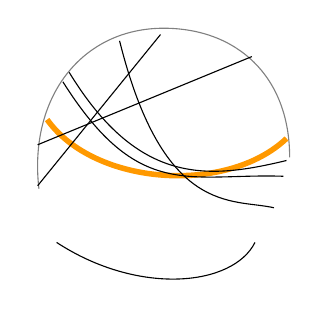
\begin{tikzpicture}[x=.8cm,y=.8cm]
\draw[gray] (.12,1.65)..controls(-.05,3.1)and(.8,4.2)..(2.1,4.2)..controls(3.25,4.2)and(4.1,3.45)..(4.1,2.15);
\draw[orange!80!yellow,line width=2pt] (.25,2.75) .. controls (1,1.7) and (3.1,1.55) .. (4.05,2.45);
\draw (.1,1.7)--(2.05,4.1);
\draw (.1,2.35)--(3.5,3.75);
\draw (.5,3.35) .. controls (1.7,1.45) and (2.5,1.9) .. (4,1.85);
\draw (.6,3.5) .. controls (1.7,1.7) and (2.8,1.8) .. (4.05,2.1);
\draw (1.4,4) .. controls (2.1,1.2) and (3.2,1.5) .. (3.85,1.35);
\draw (.4,.8) .. controls (1.7,-.05) and (3.2,.1) .. (3.55,.8);
\end{tikzpicture}}
\figure{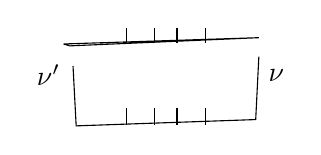
\begin{tikzpicture}[x=.8cm,y=.8cm]
\draw (0,1.3)--(3.1,1.4)--(.1,1.27)--(0,1.3);
\draw (.15,.95)--(.2,0)--(3.05,.1)--(3.1,1.1);
\foreach \x in {1,1.45,1.8,2.25}{\draw (\x,1.32)--(\x,1.55);\draw (\x,.02)--(\x,.28);}
\node[left] at (.1,.8) {$\nu'$};
\node[right] at (3.1,.8) {$\nu$};
\end{tikzpicture}}
\figure{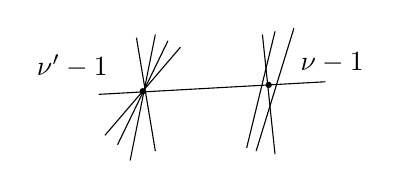
\begin{tikzpicture}[x=.8cm,y=.8cm]
\draw (0,1)--(3.6,1.2);
\fill (.7,1.05) circle (.05);\fill (2.7,1.15) circle (.05);
\draw (.6,1.9)--(.9,.1);\draw (.9,1.95)--(.5,-.05);\draw (1.1,1.85)--(.3,.2);\draw (1.3,1.75)--(.1,.35);
\draw (2.6,1.95)--(2.8,.05);\draw (2.8,2)--(2.35,.15);\draw (3.1,2.05)--(2.5,.1);
\node[left] at (.3,1.45) {$\nu'-1$};\node[right] at (3.05,1.5) {$\nu-1$};
\end{tikzpicture}}
\scanpage{85}
\figure{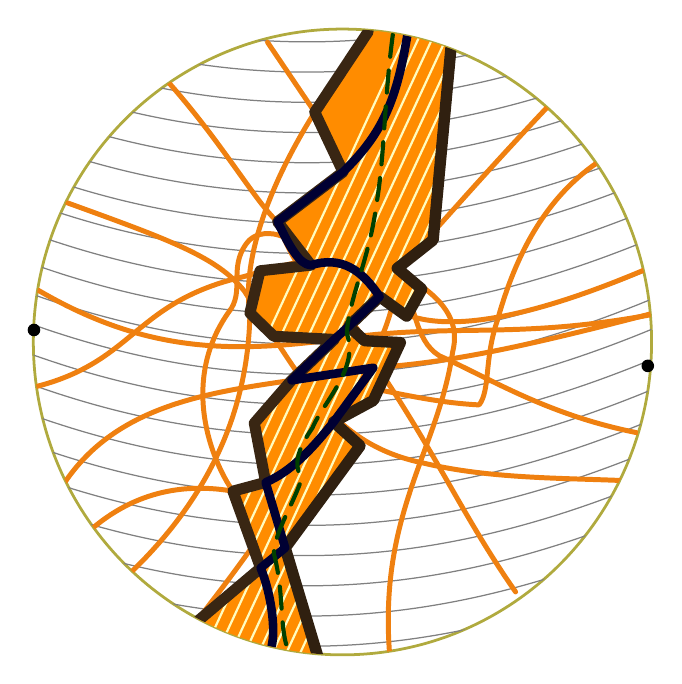
\begin{tikzpicture}[x=.008cm,y=-.008cm,line cap=round,line join=round]
\draw[yellow!65!black,line width=1pt] (763,763) ellipse (491 and 497);
\begin{scope}\clip (763,763) ellipse (491 and 497);
\draw[gray,line width=.45pt] (240,100) .. controls (610,240) and (930,210) .. (1280,60);
\draw[gray,line width=.45pt] (240,148) .. controls (610,288) and (930,258) .. (1280,108);
\draw[gray,line width=.45pt] (240,196) .. controls (610,336) and (930,306) .. (1280,156);
\draw[gray,line width=.45pt] (240,244) .. controls (610,384) and (930,354) .. (1280,204);
\draw[gray,line width=.45pt] (240,292) .. controls (610,432) and (930,402) .. (1280,252);
\draw[gray,line width=.45pt] (240,340) .. controls (610,480) and (930,450) .. (1280,300);
\draw[gray,line width=.45pt] (240,388) .. controls (610,528) and (930,498) .. (1280,348);
\draw[gray,line width=.45pt] (240,436) .. controls (610,576) and (930,546) .. (1280,396);
\draw[gray,line width=.45pt] (240,484) .. controls (610,624) and (930,594) .. (1280,444);
\draw[gray,line width=.45pt] (240,532) .. controls (610,672) and (930,642) .. (1280,492);
\draw[gray,line width=.45pt] (240,580) .. controls (610,720) and (930,690) .. (1280,540);
\draw[gray,line width=.45pt] (240,628) .. controls (610,768) and (930,738) .. (1280,588);
\draw[gray,line width=.45pt] (240,676) .. controls (610,816) and (930,786) .. (1280,636);
\draw[gray,line width=.45pt] (240,724) .. controls (610,864) and (930,834) .. (1280,684);
\draw[gray,line width=.45pt] (240,772) .. controls (610,912) and (930,882) .. (1280,732);
\draw[gray,line width=.45pt] (240,820) .. controls (610,960) and (930,930) .. (1280,780);
\draw[gray,line width=.45pt] (240,868) .. controls (610,1008) and (930,978) .. (1280,828);
\draw[gray,line width=.45pt] (240,916) .. controls (610,1056) and (930,1026) .. (1280,876);
\draw[gray,line width=.45pt] (240,964) .. controls (610,1104) and (930,1074) .. (1280,924);
\draw[gray,line width=.45pt] (240,1012) .. controls (610,1152) and (930,1122) .. (1280,972);
\draw[gray,line width=.45pt] (240,1060) .. controls (610,1200) and (930,1170) .. (1280,1020);
\draw[gray,line width=.45pt] (240,1108) .. controls (610,1248) and (930,1218) .. (1280,1068);
\draw[gray,line width=.45pt] (240,1156) .. controls (610,1296) and (930,1266) .. (1280,1116);
\draw[gray,line width=.45pt] (240,1204) .. controls (610,1344) and (930,1314) .. (1280,1164);
\draw[gray,line width=.45pt] (240,1252) .. controls (610,1392) and (930,1362) .. (1280,1212);
\draw[gray,line width=.45pt] (240,1300) .. controls (610,1440) and (930,1410) .. (1280,1260);
\draw[gray,line width=.45pt] (240,1348) .. controls (610,1488) and (930,1458) .. (1280,1308);
\draw[gray,line width=.45pt] (240,1396) .. controls (610,1536) and (930,1506) .. (1280,1356);
\draw[orange!75!brown,line width=1.8pt] (487,351) .. controls (573,448) and (628,545) .. (660,572) .. controls (683,644) and (750,724) .. (773,738) .. controls (902,915) and (943,1024) .. (1038,1160);
\draw[orange!75!brown,line width=1.8pt] (644,287)--(719,398) .. controls (625,548) and (606,658) .. (616,717) .. controls (613,909) and (518,1042) .. (425,1131);
\draw[orange!75!brown,line width=1.8pt] (1096,382) .. controls (947,539) and (885,619) .. (850,646) .. controls (847,757) and (781,827) .. (749,890) .. controls (635,1078) and (569,1156) .. (530,1209);
\draw[orange!75!brown,line width=1.8pt] (1174,474) .. controls (1088,530) and (1039,621) .. (1009,729) .. controls (988,790) and (998,840) .. (980,863) .. controls (865,857) and (785,821) .. (682,824) .. controls (545,844) and (400,865) .. (318,992);
\draw[orange!75!brown,line width=1.8pt] (326,542) .. controls (489,601) and (564,628) .. (607,682) .. controls (695,816) and (745,925) .. (890,955) .. controls (994,980) and (1108,979) .. (1204,983);
\draw[orange!75!brown,line width=1.8pt] (280,681) .. controls (441,775) and (574,783) .. (750,759) .. controls (940,731) and (1030,761) .. (1257,719);
\draw[orange!75!brown,line width=1.8pt] (272,835) .. controls (435,795) and (429,700) .. (607,659) .. controls (744,619) and (768,617) .. (822,691) .. controls (871,746) and (991,755) .. (1244,648);
\draw[orange!75!brown,line width=1.8pt] (359,1065) .. controls (436,996) and (519,988) .. (589,1000) .. controls (725,1000) and (799,821) .. (798,761) .. controls (780,722) and (718,682) .. (713,641) .. controls (691,588) and (631,578) .. (611,606) .. controls (581,646) and (609,683) .. (582,716) .. controls (504,827) and (556,953) .. (589,1000);
\draw[orange!75!brown,line width=1.8pt] (1254,718) .. controls (1028,777) and (924,796) .. (812,804) .. controls (764,811) and (730,820) .. (682,824);
\draw[orange!75!brown,line width=1.8pt] (1230,907) .. controls (1086,878) and (998,821) .. (917,785) .. controls (876,760) and (880,701) .. (850,646) .. controls (871,668) and (958,701) .. (938,779) .. controls (915,935) and (820,1035) .. (838,1260);
\fill[orange!90!yellow] (804,270)--(719,398)--(764,493)--(660,572)--(713,641)--(632,650)--(616,717)--(654,754)--(750,759)--(682,824)--(623,892)--(641,986)--(589,1000)--(633,1122)--(530,1209) .. controls (589,1242) and (650,1257) .. (724,1263)--(672,1090)--(791,928)--(749,890)--(812,856)--(855,764)--(798,761)--(773,738)--(822,691)--(865,722)--(889,679)--(850,646)--(907,601)--(936,289) .. controls (888,276) and (845,267) .. cycle;
\begin{scope}\clip (804,270)--(719,398)--(764,493)--(660,572)--(713,641)--(632,650)--(616,717)--(654,754)--(750,759)--(682,824)--(623,892)--(641,986)--(589,1000)--(633,1122)--(530,1209) .. controls (589,1242) and (650,1257) .. (724,1263)--(672,1090)--(791,928)--(749,890)--(812,856)--(855,764)--(798,761)--(773,738)--(822,691)--(865,722)--(889,679)--(850,646)--(907,601)--(936,289) .. controls (888,276) and (845,267) .. cycle;
\draw[yellow!25,line width=.8pt] (390,1300)--(890,220);
\draw[yellow!25,line width=.8pt] (412,1300)--(912,220);
\draw[yellow!25,line width=.8pt] (434,1300)--(934,220);
\draw[yellow!25,line width=.8pt] (456,1300)--(956,220);
\draw[yellow!25,line width=.8pt] (478,1300)--(978,220);
\draw[yellow!25,line width=.8pt] (500,1300)--(1000,220);
\draw[yellow!25,line width=.8pt] (522,1300)--(1022,220);
\draw[yellow!25,line width=.8pt] (544,1300)--(1044,220);
\draw[yellow!25,line width=.8pt] (566,1300)--(1066,220);
\draw[yellow!25,line width=.8pt] (588,1300)--(1088,220);
\draw[yellow!25,line width=.8pt] (610,1300)--(1110,220);
\draw[yellow!25,line width=.8pt] (632,1300)--(1132,220);
\draw[yellow!25,line width=.8pt] (654,1300)--(1154,220);
\draw[yellow!25,line width=.8pt] (676,1300)--(1176,220);
\draw[yellow!25,line width=.8pt] (698,1300)--(1198,220);
\draw[yellow!25,line width=.8pt] (720,1300)--(1220,220);
\draw[yellow!25,line width=.8pt] (742,1300)--(1242,220);
\draw[yellow!25,line width=.8pt] (764,1300)--(1264,220);
\draw[yellow!25,line width=.8pt] (786,1300)--(1286,220);
\draw[yellow!25,line width=.8pt] (808,1300)--(1308,220);
\draw[yellow!25,line width=.8pt] (830,1300)--(1330,220);
\draw[yellow!25,line width=.8pt] (852,1300)--(1352,220);
\draw[yellow!25,line width=.8pt] (874,1300)--(1374,220);
\draw[yellow!25,line width=.8pt] (896,1300)--(1396,220);
\draw[yellow!25,line width=.8pt] (918,1300)--(1418,220);
\draw[yellow!25,line width=.8pt] (940,1300)--(1440,220);
\draw[yellow!25,line width=.8pt] (962,1300)--(1462,220);
\draw[yellow!25,line width=.8pt] (984,1300)--(1484,220);
\draw[yellow!25,line width=.8pt] (1006,1300)--(1506,220);
\draw[yellow!25,line width=.8pt] (1028,1300)--(1528,220);
\draw[yellow!25,line width=.8pt] (1050,1300)--(1550,220);
\draw[yellow!25,line width=.8pt] (1072,1300)--(1572,220);
\draw[yellow!25,line width=.8pt] (1094,1300)--(1594,220);
\end{scope}
\draw[brown!30!black,line width=4pt] (804,270)--(719,398)--(764,493)--(660,572)--(713,641)--(632,650)--(616,717)--(654,754)--(750,759)--(682,824)--(623,892)--(641,986)--(589,1000)--(633,1122)--(530,1209);
\draw[brown!25!black,line width=4.1pt] (936,289)--(907,601)--(850,646)--(889,679)--(865,722)--(822,691)--(773,738)--(798,761)--(855,764)--(812,856)--(749,890)--(791,928)--(672,1090)--(724,1263);
\draw[blue!20!black,line width=3.1pt] (866,276) .. controls (848,386) and (823,435) .. (764,493)--(660,572) .. controls (678,610) and (695,641) .. (713,641) .. controls (762,626) and (794,649) .. (822,691)--(773,738)--(750,759)--(682,824)--(812,804)--(749,890) .. controls (713,935) and (681,969) .. (641,986)--(672,1090)--(633,1122) .. controls (649,1160) and (658,1220) .. (650,1248);
\draw[green!25!black,line width=1.5pt,dash pattern=on 8pt off 5pt] (843,275) .. controls (829,380) and (830,468) .. (817,544) .. controls (806,631) and (772,697) .. (770,750) .. controls (790,804) and (733,858) .. (715,900) .. controls (676,956) and (697,969) .. (697,984) .. controls (680,1030) and (656,1065) .. (654,1099) .. controls (670,1159) and (663,1211) .. (675,1248);
\end{scope}
\fill (273,744) circle (10);
\fill (1248,801) circle (10);
\end{tikzpicture}}
% crop-candidate: scan 85
\margin{84}
\scanpage{86}
\uline{5.1.84}

J'ai vérifié que si $\mathcal X$ désigne la
surface des pos. rel. non supersingulières,
sans bord en permettant le franchissement
des positions supersingulières
par une arête ou par un sommet
(\unsure{copulations} des \uline{poids $0$}), alors que les
autres opérations qui \unsure{s'y interprètent}
par le côté, \unsure{donnent|donne} les spéc. et gén.
ordinaires (i.e. des poids $\pm1$) --- alors
\[
\pi_1(\mathcal X,D)\longrightarrow\mathbb D_{2n}
\quad\text{(en fait : }\operatorname{Aut}\operatorname{Pol}(\unsure{D_{\mathrm{am}}})\text{)}
\]
était surjectif --- son image contient,
pour une arête ou un \deleted{\unsure{g}} sommet
donné en $D$, la symétrie p.r.
cette arête ou sommet, par le lacet
corresp. et à une ``\uline{demi torsion}'' de $D$
autour du \deleted{\unsure{cet}} sommet, ou cette
arête. Ceci ne prouve pas que
\[
\pi_1(\widetilde{\mathcal X},D)\longrightarrow
\operatorname{Aut}\operatorname{Pol}(D)\simeq\mathbb D_{2n}
\]
soit surjectif, si $\widetilde{\mathcal X}$ désigne le \unsure{découpage}
de $\mathcal X$ le long des lieux supercritiques
--- i.e. en exclut le franchissement des
positions supersingulières. Le raisonnement
montre seulement que l'image contient
les symétries p.r. à \deleted{\unsure{l'autre}} \uline{arête} (mais pas
néc. p.r. à un sommet). \deleted{\unsure{Celles symétries}}
engendrent ds $\mathbb D_{2n}$ un \deleted{sous} groupe
d'indice $2$, à savoir celui formé par les
\deleted{rotations} les élts du sous-groupe
de rotations $\mathbb D_n^+$ (d'ordre \uline{$n$}, non $2n$),
et les réflexions en question. [NB. C'est
un des trois sous-groupes d'indice deux,
les deux autres étant le groupe engendré
par les \deleted{\unsure{sym}} réflexions qui \unsure{inversent} \deleted{\unsure{les}}
un sommet, et le sous-groupe $\mathbb D_{2n}^+$
des rotations.] L'image de $\pi_1(\widetilde{\mathcal X})$ ds $\mathbb D_{2n}$
est donc d'indice $1$ ou $2$.

Faisant un \deleted{\unsure{demi tour}} \inserted{demi} tour \deleted{complet}
autour d'une position supersingulière,
\inserted{par le franchissement, \unsure{tout des effets sur}}
\deleted{\unsure{dans l'opération de rotation par}}
\inserted{(sur $\operatorname{Pol}(D)$) qui \unsure{se fait|définit} par une rotation}
\deleted{\unsure{(sur) un cercle par $\pi/2$}, \unsure{fait une} \uline{\unsure{demi}}}
\deleted{\unsure{tour}} \inserted{d'un facteur} \unsure{$n+1$} --- si $n$ est \deleted{pair}
impair, cela montre que l'effet sur
l'ensemble \deleted{des \unsure{p.}} \inserted{$\varepsilon_a(D)$} des \deleted{\unsure{poly}}gones
circonscrits (et aussi sur les deux autres
ens. à deux éléments $\varepsilon_s(D)$, $\uline{\omega}(D)$)
est le $=$. \deleted{\unsure{que}} Donc pour voir si $\forall$
lacet en $D_0$ \deleted{fixé}, donne \deleted{fixe}

\margin{\unsure{J'ai été assez négligent}
\unsure{dans l'explicitation de la règle}
\unsure{de recollement des flèches} de transition
exceptionnelles.}
\margin{\unsure{reste trop conjectural}; \unsure{en fait} $\deleted{\unsure{+}}1$ \unsure{au lieu} \unsure{de}
\unsure{l'angle} \unsure{ci-dessus}. \unsure{Mais c'est l'angle}.}
\figure{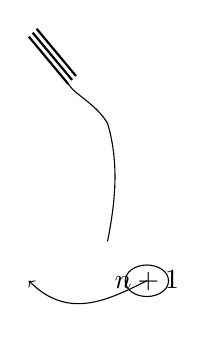
\begin{tikzpicture}[x=.5cm,y=.5cm]
\draw (0,0)..controls(.2,1)and(.3,2)..(0,3);
\draw (0,3)..controls(-.3,3.5)and(-.8,3.7)..(-1,4);
\draw[line width=.8pt](-1,4)--(-2,5.2) (-.9,4.1)--(-1.9,5.3) (-.8,4.2)--(-1.8,5.4);
\draw[->](1,-1)..controls(0,-1.5)and(-1,-2)..(-2,-1);
\draw (1,-1) ellipse(.55 and .4);
\node at (1,-1){$n+1$};
\end{tikzpicture}}
\margin{85}
\scanpage{87}
induit l'identité sur $\varepsilon_a(D_0)$, il revient au
$=$ de se permettre de franchir les
positions supersingulières, or on a :
donc pour $n$ impair, $\pi_1(\widetilde{\mathcal X}\unsure{,|)}\longrightarrow\mathbb D_{2n}$
est aussi surjectif. Si $n$ est
pair, le résultat \inserted{sur $\varepsilon_a(D_0)$} d'un lacet $l$
\deleted{obtenu} ds $\mathcal X$ qui franchit
$\nu$ fois une position supersingulière,
est, \inserted{suivant que $\nu$ est pair ou impair,} le $=$ resp. opposé à celui obtenu
par le lacet $l'$ qui se déduit de
$l$ en remplaçant les franchissements
par des demi-tours. Si donc on
\deleted{prend} part d'une c. pos. rel. $D_0$ qui
passe par un sommet \inserted{$s_0$ de} $\Sigma$ \uline{d'ordre}
\uline{pair}, alors en modifiant le lacet $l$
demi-tour \inserted{de $D_0$} autour de $s_0$, de la
façon indiquée, on trouve une
\deleted{\unsure{autre}} action \deleted{\unsure{de}} $\varepsilon(D_0)$ qui n'est
pas l'identité. Cela prouve donc que
\uline{dans tous les cas}, $\pi_1(\widetilde{\mathcal X}\unsure{,|)}\longrightarrow\mathbb D_{2n}$ est
surjectif --- i.e. le revêt \inserted{principal associé} de $\unsure{\widetilde{\mathcal X}|\mathcal X}$, de groupe
$\mathbb D_{2n}$ est \uline{connexe}.
\margin{86}
\scanpage{88}
5.1.84

Soit $X$ une surface compacte, munie
d'un graphe topologique $X_1\subset X$ la
décomposant cellulairement. [On s'intéressera
plus particulièrement au cas où
\deleted{\unsure{tous}} les vts de $X_1$ sont d'ordre pair, p.e.
$(X,X_1)$ est un syst. de pseudo-droites
ds un plan \deleted{\unsure{p}} projectif réel topologique.]
\deleted{Soit} Un cercle topologique $D\subset X$ sera dit
``en \unsure{posit.}, \unsure{standard|standart}'' (p.r. à $X_1$), s'il
\deleted{\unsure{n'est en}} rencontre $X_1$, et si pour $\forall$
$a\in X_1\cap D$, \deleted{$D$ \uline{croise} \unsure{toutes les}} $a$ est un
pt d'ordre pair de $X_1$, et $D$ \uline{croise} ttes
branches de $X_1$ en $a$. On dit que deux
tels $D,D'$ sont ``en $=$ \unsure{position relative}''
ou sont \uline{isotopes}, si on peut passer
\inserted{(par des paramétrisations continues $D\simeq\unsure{\mathrm U|\mathrm U_1}$, $D'\simeq\unsure{\mathrm U|\mathrm U_1}$)}
de $D$ à $D'$ par une ``isotopie'', au cours
de laquelle, non seulement les positions
intermédiaires $D_t$ sont en position st.
mais en plus $D_t\cap S(\unsure{K|X})$ reste constant.
Il f. et s. pour cela que, \deleted{\unsure{pour}} \inserted{désignant} par
$\unsure{\Phi|\mathcal F}(D)$ l'ens. des facettes de $(X,X_1)$ rencontrées
par $D$, que l'on ait $\unsure{\Phi|\mathcal F}(D)=\unsure{\Phi|\mathcal F}(D')$. Il f. et s.
aussi qu'il existe une famille à un
paramètre $f_t$ $(0\leq t\leq1)$ d'autom. de
$(X,X_1)$, avec $f_0=\mathrm{id}$, et $f_1(D)=D'$.

On définit une notion de \uline{balayage} d'une
p.r. au dessus d'un sommet \uline{pair} de $X_1$,
comme dans le cas des syst. de ps. dr.,
et une notion correspondante de
spécialisation vers un sommet. \deleted{Également,
la notion de}
Pour $D$ donné, les op. de spéc. et de
généralis. à partir de $D$ se \unsure{repèrent}
encore p. des ``arcs de \deleted{balayage} \inserted{transition}'', sur
\deleted{\unsure{de}} la réu. $\widetilde D$ des rives de $D$, qui
\figure{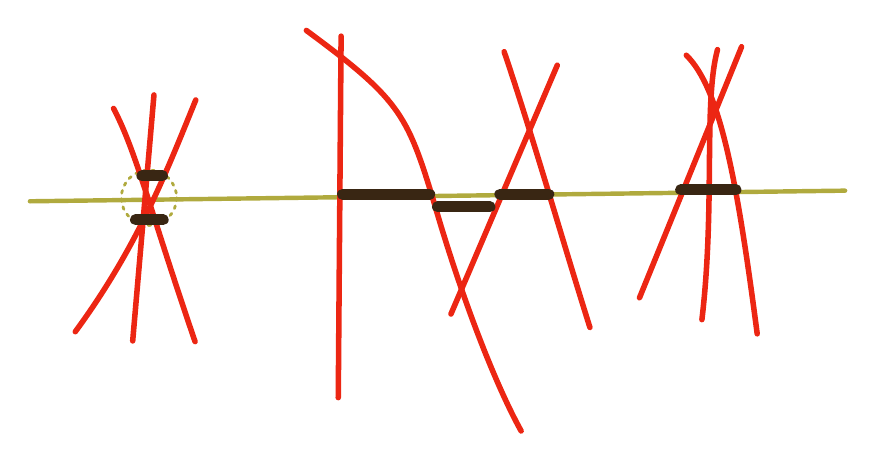
\begin{tikzpicture}[x=.009cm,y=-.009cm,line cap=round,line join=round]
\draw[yellow!65!black,line width=1.6pt](1600,1200)--(2750,1185);
\draw[yellow!65!black,line width=1pt,dotted](1768,1195) circle(39);
\draw[red!70!brown,line width=2pt](1718,1069)..controls(1750,1130)and(1769,1211)..(1833,1398);
\draw[red!70!brown,line width=2pt](1775,1050)--(1745,1397);
\draw[red!70!brown,line width=2pt](1834,1057)..controls(1792,1160)and(1752,1264)..(1664,1384);
\draw[brown!30!black,line width=4pt](1758,1164)--(1787,1164) (1749,1226)--(1788,1226);
\draw[red!70!brown,line width=2pt](2039,967)--(2035,1477);
\draw[red!70!brown,line width=2pt](1990,959)..controls(2120,1055)and(2132,1076)..(2169,1198)..controls(2210,1340)and(2258,1461)..(2293,1524);
\draw[red!70!brown,line width=2pt](2344,1008)--(2194,1359);
\draw[red!70!brown,line width=2pt](2269,989)..controls(2310,1110)and(2350,1251)..(2390,1378);
\draw[brown!30!black,line width=4pt](2041,1190)--(2164,1190) (2175,1208)--(2249,1208) (2263,1190)--(2332,1190);
\draw[red!70!brown,line width=2pt](2526,994)..controls(2573,1040)and(2597,1165)..(2626,1387);
\draw[red!70!brown,line width=2pt](2570,986)..controls(2550,1060)and(2567,1206)..(2548,1367);
\draw[red!70!brown,line width=2pt](2604,982)--(2460,1336);
\draw[brown!30!black,line width=4pt](2518,1184)--(2596,1184);
\end{tikzpicture}}
forment, en se recollant, une
famille d'arcs \deleted{\unsure{puis}} \inserted{\unsure{dont les adh.}} sont deux à deux disjoints.
Il y a une notion de transport parallèle
pour $\widetilde D$, munie de sa structure de
contour \inserted{top.} naturelle (ou plutôt, pour
sa structure combinatoire) pour tte
généralis. de spéc. en gén., et aussi
\margin{87}
\scanpage{89}
\figure{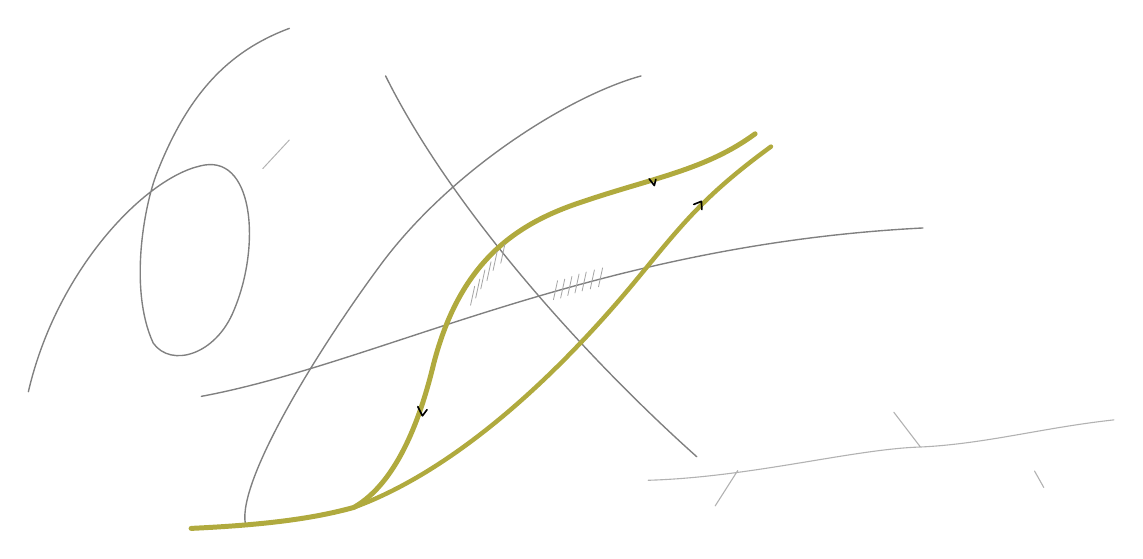
\begin{tikzpicture}[x=.0065cm,y=-.0065cm,line cap=round,line join=round]
\draw[gray,line width=.5pt](266,775)..controls(321,537)and(493,359)..(601,334)..controls(705,306)and(722,486)..(668,615)..controls(633,703)and(545,729)..(510,680)..controls(462,576)and(492,412)..(517,348)..controls(577,195)and(655,110)..(776,65);
\draw[gray,line width=.5pt](690,1033)..controls(674,947)and(838,682)..(961,518)..controls(1099,337)and(1325,196)..(1463,158);
\draw[gray,line width=.5pt](964,158)..controls(1093,418)and(1355,708)..(1572,902);
\draw[gray,line width=.5pt](604,784)..controls(954,719)and(1370,488)..(2014,455);
\draw[gray!60,line width=.4pt](1477,948)..controls(1678,942)and(1878,887)..(2009,883)..controls(2136,877)and(2249,845)..(2387,830) (1957,815)--(2009,883) (1652,929)--(1608,998) (2232,930)--(2250,962);
\draw[yellow!65!black,line width=1.8pt](584,1042)..controls(734,1035)and(826,1022)..(902,1001)..controls(991,950)and(1035,815)..(1058,720)..controls(1111,515)and(1225,444)..(1351,403)..controls(1487,357)and(1591,341)..(1686,271);
\draw[yellow!65!black,line width=1.6pt](902,1001)..controls(1104,927)and(1299,741)..(1441,572)..controls(1536,458)and(1576,399)..(1717,296);
\draw[black,line width=.6pt](1027,804)--(1036,822)--(1045,810) (1479,359)--(1489,372)--(1492,360) (1566,409)--(1581,403)--(1582,419);
\draw[gray!70,line width=.3pt](1130,606)--(1138,569);
\draw[gray!70,line width=.3pt](1140,592)--(1148,555);
\draw[gray!70,line width=.3pt](1150,574)--(1158,537);
\draw[gray!70,line width=.3pt](1162,558)--(1170,521);
\draw[gray!70,line width=.3pt](1174,538)--(1182,501);
\draw[gray!70,line width=.3pt](1189,524)--(1197,487);
\draw[gray!70,line width=.3pt](1292,595)--(1300,558);
\draw[gray!70,line width=.3pt](1306,592)--(1314,555);
\draw[gray!70,line width=.3pt](1320,587)--(1328,550);
\draw[gray!70,line width=.3pt](1334,582)--(1342,545);
\draw[gray!70,line width=.3pt](1348,578)--(1356,541);
\draw[gray!70,line width=.3pt](1364,574)--(1372,537);
\draw[gray!70,line width=.3pt](1380,570)--(1388,533);
\draw[gray!60,line width=.35pt](724,339)--(776,283);
\end{tikzpicture}}
\margin{88}
\scanpage{90}
Pour tte famille à $1$ paramètre de $D$
qui se décompose en segments
tels qu'à l'intérieur de chacun
d'eux les p.r. reste \unsure{constant} et
\deleted{\unsure{de que}} qu'aux extrémités se
trouve encore des $D_t$ qui restent
en position \unsure{standard|standart}).

On se restreindra maintenant au
cas des p.r. à une seule rive ---
i.e. telles que $\widetilde D$ soit un cercle top.
Alors l'ens. des op. de transition à
partir de $D$ est muni d'une
structure polygonale \inserted{(\unsure{c.à.d.} de deux façons, suivant convention pour
\unsure{rives} de généralisation)}. Donc le graphe \inserted{orienté}
des p.r. est polygonalisé, et \deleted{\unsure{d'où}} \unsure{donc|de même}
deux façons de définir des op. de
transport pour l'orientation. La convention
la plus intéressante semble celle où la
rive de généralisation ``tire'' sur $D$ pour génériser,
et que le transport de l'orientation sur
$\mathcal X$ soit opposé au transport parallèle de
l'orientation.

Dans ce cas, dans la carte $\mathcal X$ obtenue,
tous les sommets sont d'ordre
$4$, et ils correspondent \deleted{\unsure{ainsi}} \inserted{$1$-$1$} aux
\deleted{p.r. $D$} $(D,\deleted{\unsure{\xi}}a)$, où $D$ est
une p.r., et $a$ un ``arc d'\unsure{inertie}''
sur $\widetilde D$, de type générique i.e.
joignant deux \deleted{sommets} \inserted{pts} de $D\cap S(X_1)$
(\unsure{c.à.d.} que son \unsure{intérieur|extérieur} ne rencontre
ni d'autre élément de $S(X_1)$, ni de \unsure{rive}
de spécialisation).
La situation est surtout sympathique
si la découpe de $X$ suivant les
positions relatives envisagées est un
disque (cela peut signifier aussi
que $X$ est un plan projectif
réel, et $D$ une ps droite) ---
condition qui est invariante par
opérations élémentaires, car
alors on peut interpréter $\mathcal X$ comme
\unsure{déduite} de ces découpes par des
\unsure{recollements}, et on récupère des
\margin{89}
\scanpage{91}
\texttt{//*\quad GUTS\quad 0108\qquad\unsure{I|1}}
\figure{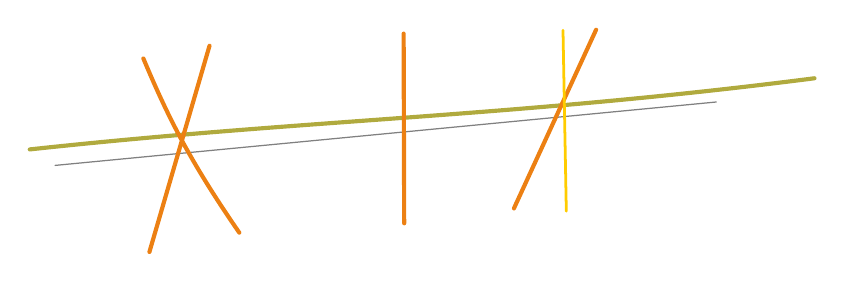
\begin{tikzpicture}[x=.007cm,y=-.007cm,line cap=round]
\draw[yellow!65!black,line width=1.5pt](320,406)..controls(827,351)and(1188,348)..(1743,277);
\draw[gray,line width=.45pt](366,435)--(1565,320);
\draw[orange!70!brown,line width=1.5pt](526,241)..controls(572,351)and(613,431)..(700,557) (646,218)--(537,592) (998,196)--(999,540) (1347,189)--(1198,513);
\draw[orange!40!yellow,line width=1pt](1287,190)--(1293,518);
\end{tikzpicture}}
\begin{verbatim}
 GGGGGGGGGG   UU        UU  TTTTTTTTTTTT   SSSSSSSSSS
GGGGGGGGGGGG  UU        UU  TTTTTTTTTTTT  SSSSSSSSSSSS
GG        GG  UU        UU       TT       SS        SS
GG            UU        UU       TT       SS
GG            UU        UU       TT       SSS
GG            UU        UU       TT        SSSSSSSSS
GG     GGGGG  UU        UU       TT         SSSSSSSSS
GG     GGGGG  UU        UU       TT                SSS
GG        GG  UU        UU       TT                 SS
GG        GG  UU        UU       TT       SS        SS
GGGGGGGGGGGG  UUUUUUUUUUUU       TT       SSSSSSSSSSSS
 GGGGGGGGGG    UUUUUUUUUU        TT        SSSSSSSSSS
\end{verbatim}
\diagram{\begin{array}{llllllllllllllllll}
\mathtt{****P}&\mathtt{END}&\mathtt{STC}&\mathtt{108}&\mathtt{GUTS}&\mathtt{ROOM}&\mathtt{3.44.20}&\mathtt{PM}&\mathtt{16}&\mathtt{AUG}&\mathtt{82}&\mathtt{R6.PR1}&\mathtt{SYS}&\mathtt{JES2}&\mathtt{STC}&\mathtt{108}&\mathtt{END}&\mathtt{P****}\\
\mathtt{****P}&\mathtt{END}&\mathtt{STC}&\mathtt{108}&\mathtt{GUTS}&\mathtt{ROOM}&\mathtt{3.44.20}&\mathtt{PM}&\mathtt{16}&\mathtt{AUG}&\mathtt{82}&\mathtt{R6.PR1}&\mathtt{SYS}&\mathtt{JES2}&\mathtt{STC}&\mathtt{108}&\mathtt{END}&\mathtt{P****}\\
\mathtt{****P}&\mathtt{END}&\mathtt{STC}&\mathtt{108}&\mathtt{GUTS}&\mathtt{ROOM}&\mathtt{3.44.20}&\mathtt{PM}&\mathtt{16}&\mathtt{AUG}&\mathtt{82}&\mathtt{R6.PR1}&\mathtt{SYS}&\mathtt{JES2}&\mathtt{STC}&\mathtt{108}&\mathtt{END}&\mathtt{P****}\\
\mathtt{****P}&\mathtt{END}&\mathtt{STC}&\mathtt{108}&\mathtt{GUTS}&\mathtt{ROOM}&\mathtt{3.44.20}&\mathtt{PM}&\mathtt{16}&\mathtt{AUG}&\mathtt{82}&\mathtt{R6.PR1}&\mathtt{SYS}&\mathtt{JES2}&\mathtt{STC}&\mathtt{108}&\mathtt{END}&\mathtt{P****}\\
\mathtt{****P}&\mathtt{END}&\mathtt{STC}&\mathtt{108}&\mathtt{GUTS}&\mathtt{ROOM}&\mathtt{3.44.20}&\mathtt{PM}&\mathtt{16}&\mathtt{AUG}&\mathtt{82}&\mathtt{R6.PR1}&\mathtt{SYS}&\mathtt{JES2}&\mathtt{STC}&\mathtt{108}&\mathtt{END}&\mathtt{P****}\\
\mathtt{****P}&\mathtt{END}&\mathtt{STC}&\mathtt{108}&\mathtt{GUTS}&\mathtt{ROOM}&\mathtt{3.44.20}&\mathtt{PM}&\mathtt{16}&\mathtt{AUG}&\mathtt{82}&\mathtt{R6.PR1}&\mathtt{SYS}&\mathtt{JES2}&\mathtt{STC}&\mathtt{108}&\mathtt{END}&\mathtt{P****}
\end{array}}
\diagram{\begin{tikzcd}[ampersand replacement=\&,column sep=large,row sep=large]
\text{a) Rives marquées}\arrow[r,Rightarrow]\arrow[dd,leftrightarrow,bend right=65,double]
\&\text{a') \deleted{angles} \inserted{coins} marqués}\\
\text{b) arcs contigus marqués sur les arêtes}\arrow[u,Rightarrow]\&\\
\text{c) \uline{poids} des faces}\&
\end{tikzcd}}
\margin{90}
\scanpage{92}
$\mathcal X$ un graphe topologique $L$ comme
à l'accoutumée. Mais alors $=$
que les $\operatorname{Dec}(X,D)$ ne seraient pas
des disques, et sans $=$ supposer $\widetilde D$
connexe, on peut construire une
\inserted{nouvelle} surface \inserted{$\mathcal X'$, avec un graphe top. $K'$ dans $\unsure{\mathcal X|\mathcal X'}$}
en recollant toutes les
découpes --- mais $(\mathcal X',K')$ n'est plus
néc. cellulaire, il faut y prendre
$L'$ et prendre $(\mathcal X',K'\cup L')$ pour avoir
qqque chose de cellulaire.

Tantôt en disant que les sommets \inserted{de $\unsure{(\mathcal X,K)|K}$}
sont d'ordre $4$, j'ai été un peu vite ---
il y a une exception, quand on
\deleted{\unsure{a la}} \inserted{part d'une} situation \deleted{\unsure{de}}, où \deleted{\unsure{$s$}} \deleted{\unsure{$\longleftrightarrow$}} l'arc
\figure{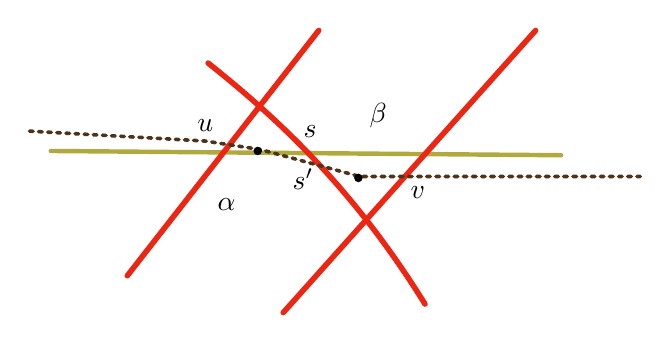
\begin{tikzpicture}[x=.018cm,y=-.018cm,line cap=round]
\draw[yellow!65!black,line width=1.6pt](365,1590)--(725,1593);
\draw[red!70!brown,line width=2pt](419,1678)--(554,1505) (476,1528)..controls(534,1574)and(583,1624)..(629,1698) (529,1704)--(707,1505);
\draw[brown!40!black,line width=1.3pt,dotted](350,1576)--(474,1583)--(513,1589)--(583,1608)--(781,1608);
\fill (511,1590) circle(3);\fill(582,1609)circle(3);
\node at(474,1572){$u$};\node at(489,1628){$\alpha$};\node at(596,1565){$\beta$};
\node at(548,1576){$s$};\node at(543,1610){$s'$};\node at(624,1619){$v$};
\end{tikzpicture}}
$\unsure{\overrightarrow{uv}|\widehat{uv}}$ (pointillé) sur
$\widetilde D_x$ est un arc
d'inertie (position
relative \uline{stable} donc). La circonstance
\unsure{propre} dans le cas où $(X,X_1)$ est un syst.
de ps. droites, et qui permet le contrôle
de ces sommets sur $\mathcal X$, est la suivante

\deleted{(PS) Soit $D$ une p.r. \deleted{\unsure{Étant} \unsure{le long duquel}
\uline{de ps dr} soit $s\in D\cap X_1$, et considérons
\unsure{le côté qui} \unsure{le} \unsure{$s',s''$} \inserted{antipolaires} \unsure{à} $s$ sur $D$, et un des arcs
déterminés \deleted{par} par $s',s''$ (appelons un
tel arc un \uline{demi-cercle} du polygone
top. ou comb. envisagé $\operatorname{Pol}(D)$), alors
\deleted{\unsure{on est sûr d'un demi-cercle}}\deleted{\unsure{sur $D$}}
\uline{si} sur $a$ il n'y a pas d'arc de
transition (``ordinaire'') alors $s\in X_0=S(X_1)$
etc.}
Soit $a$ un arc de transition \inserted{(ordinaire)}
sur $\widetilde D$, $a'$ l'arc opposé (donc $\bar a\cap\bar a'=\varnothing$)
et considérons \deleted{les} une des \inserted{$b$} comp. conn.
de $\widetilde D\setminus\{a\cup a'\}$. Alors, ou bien
$b$ contient un arc de transition \inserted{(ordinaire)}, ou
bien $b$ \deleted{\unsure{est une partie}} \inserted{est} un ``arc de
transition exceptionnel'', i.e. on est dans
l'un des cas suivants : on a une
``composante'' $D_i$ de $X_1$ qui est un cercle,
une \deleted{\unsure{sommet}} \inserted{facette $\varphi$ intermédiaire} (resp. une arête $\alpha$) sur $D_i$,
une orientation $\omega$ de $X$ en \deleted{\unsure{$\varphi$, une arête $a$ de}},
et $D$ est déduit de $(\deleted{\unsure{D_i}}\varphi,\omega)$ par
déformation élémentaire ---}
\figure{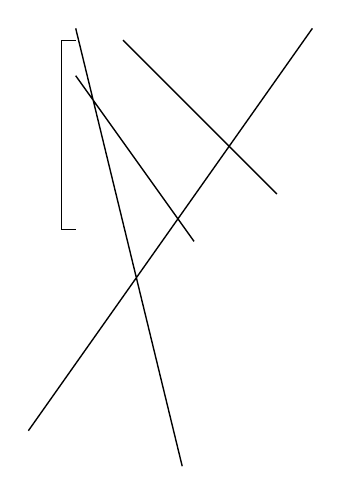
\begin{tikzpicture}[x=.003cm,y=.003cm]
\draw[line width=.5pt](0,0)--(450,-1850) (1000,0)--(-200,-1700) (200,-50)--(850,-700) (0,-200)--(500,-900);
\draw (0,-50)--(-60,-50)--(-60,-850)--(0,-850);
\end{tikzpicture}}
\margin{91}
\scanpage{93}
(\uline{PS}) Considérons un arc-demi-cercle $a$
sur $\widetilde D$ ($D$ une p.r. \uline{de ps. droite})
Alors \deleted{$\unsure{a}$}\inserted{$\mathring a$} contient un arc de transition
(ordinaire), sauf dans les \inserted{deux} cas suivants :
\margin{i.e. $a$ contient un arc de transition qui n'a pas d'extrémité en commun avec $a$.}

1°) \deleted{\unsure{Les e.}} Les extrémités $s,s'$ de $a$ \deleted{\unsure{font}} sont élts
d'arcs de généralisation \inserted{$\alpha,\alpha'$} (\unsure{néc. élts de gén.})
[i.e. le pt $\unsure{v}$ de $X$ défini par $(s,s')$ est
un sommet de $X_1$] et il y a une
composante $D_i$ de $X_1$ passant par $v$,
et une orientation $\omega$ de $X$ en $v$, tels
que $D$ soit \deleted{déduit de} ``voisin de $D_i$''
et ``déduit de $D_i$ par petite rotation,
\unsure{autour} $v$'' ; $a\setminus(\mathring\alpha\cap a)\setminus(\mathring\alpha'\cap a)$
est la rive de balayage de $D$
correspondante : $(D_i,v,\omega)$.
\margin{Cas $v\in X_0$}
\margin{\unsure{NB}}
\figure{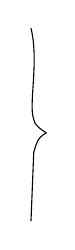
\begin{tikzpicture}[x=.35cm,y=.35cm]
\draw (0,7) .. controls (.3,5.8) and (-.1,4.2) .. (.1,3.7) .. controls (.15,3.4) and (.45,3.3) .. (.55,3.2) .. controls (.2,3) and (.2,2.8) .. (.1,2.5) -- (0,0);
\end{tikzpicture}}

2°) \deleted{Une des deux} \deleted{Les} extrémités $s,s'$ de $a$,
\deleted{\unsure{sont les}} \deleted{\unsure{élts de}} \inserted{extrémités d'}\deleted{\unsure{élts}} \deleted{\unsure{d'un}} arcs de spécialisation
$\alpha_s$, \deleted{$\unsure{\beta}$}$\alpha_{s'}$ (néc. antipodaux l'un
de l'autre !) \inserted{contenus dans $a$} \deleted{alors il existe $p,p'$}
Soit \deleted{$\unsure{\beta}$}\inserted{$\beta$}\unsure{l'arête} de $X_1$ passant par $v$, \deleted{\unsure{et}} et $D_i$
la comp. de $X_1$ contenant $\beta$, il existe
une orientation de $X$ en $\beta$ telle que
$D_i$ \unsure{déduits} —
\margin{Cas $v\notin X_0$}
\figure{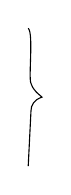
\begin{tikzpicture}[x=.35cm,y=.35cm]
\draw (0,5) .. controls (.2,4.8) and (0,3.2) .. (.1,3) .. controls (.2,2.7) and (.4,2.6) .. (.5,2.5) .. controls (.2,2.4) and (.1,2.2) .. (.1,2) -- (0,0);
\end{tikzpicture}}
\margin{\uline{NB} Dans ce cas, $a$ contient deux arcs de spécialisation,
\deleted{\unsure{de gén.}} (mais à \unsure{un côté} en commun)}

\margin{\uline{NB} Dans le cas des ps. droites, si \unsure{on a}
sur $\widetilde D$ une transition (avec \unsure{sa rive de contrebal.} en pointillés)
\figure{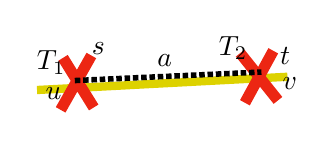
\begin{tikzpicture}[x=.6cm,y=.6cm]
\draw[yellow!70!olive,line width=3pt] (-.8,-.08)--(4.5,.2);
\draw[red!70!brown,line width=4pt] (-.3,-.5)--(.35,.65) (-.25,.6)--(.4,-.45) (3.6,-.35)--(4.2,.75) (3.5,.7)--(4.3,-.3);
\draw[black,densely dotted,line width=2pt] (0,.12)--(3.95,.3);
\node at (1.9,.55) {$a$};\node at (-.5,.5) {$\unsure{T_1}$};\node at (3.35,.8) {$\unsure{T_2}$};
\node at (.5,.8) {$s$};\node at (4.45,.65) {$t$};\node at (-.45,-.15) {$u$};\node at (4.55,.05) {$v$};
\end{tikzpicture}}
les conditions suivantes sont \inserted{équivalentes} :
a) $s,t$ \unsure{non-alignés},
b) $u\ne v'$ (\unsure{antip. de $v$})
c) dist. comb. de $u$ à $v$ est \inserted{(sur $\unsure{\widetilde D}$)} \deleted{$\unsure{\le n}$}\inserted{$\le n-1$},
d) après spécialisation \unsure{(de $T_1$)}, \unsure{en un point spécifique}, \unsure{vis. $T_2$} ($\unsure{\Leftrightarrow s=t}$)
}
\margin{\deleted{\unsure{dans le} \unsure{deux cas} \unsure{$v$ et $v'$} \unsure{sont l'unique} \unsure{comp. incid. de}}}
\figure{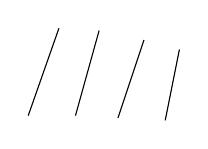
\begin{tikzpicture}[x=.3cm,y=.3cm]\draw (0,0)--(1.3,3.7) (2,0)--(3,3.6) (3.8,-.1)--(4.9,3.2) (5.8,-.2)--(6.4,2.8);\end{tikzpicture}}

C'est cette circonstance qui
suggère qu'il n'y a que
deux sortes de sommets
dans $\mathcal X$, les sommets
d'ordre 4 dont je viens de
parler, et les sommets
correspondant aux \unsure{systèmes}
$(D_i,\beta,\omega)$, où \deleted{$\unsure{\beta}$}$D_i$ est une
``composante irr. de $X_1$'' qui est un
cercle topologique dans $X$, $\beta$ une
facette de $D_i$ (sommet ou arête)
$\omega$ une orientation de $X$ en $\beta$.
Sinon, on n'a pas de contrôle, a
priori, sur le type des ``circuits-
sommets'' sur $\mathcal X$ — et \unsure{j'ajoute}
qu'il n'est pas clair \deleted{\unsure{en quoi}} dans
quelle mesure le transport
parallèle sur les $\mathrm{Pol}(D)$ \unsure{passe}
en un syst. local sur $\mathcal X$.
\margin{92}
\scanpage{94}
\figure{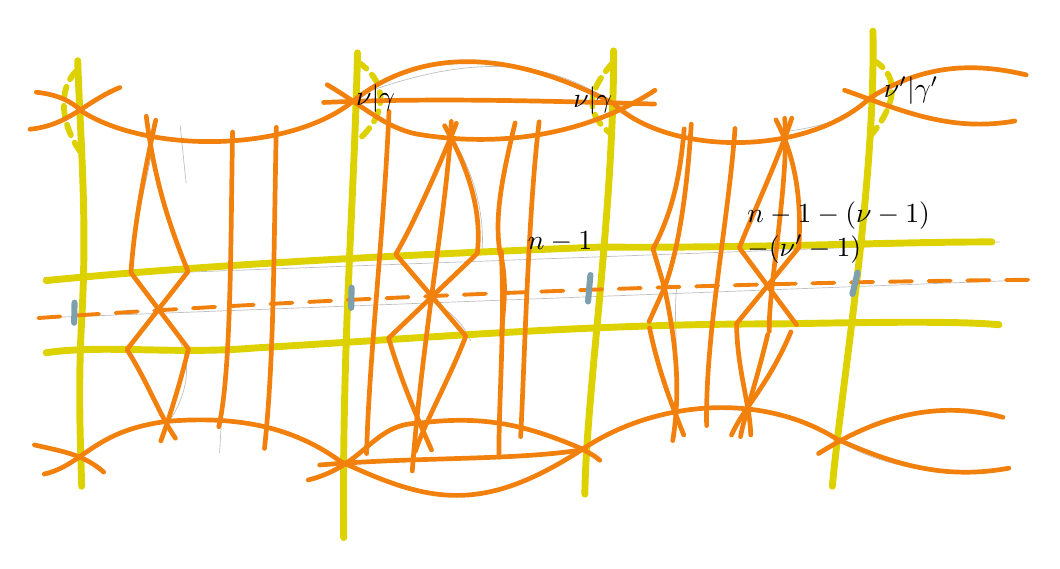
\begin{tikzpicture}[x=.005cm,y=-.005cm,line cap=round,line join=round]
\draw[gray!50,line width=.25pt] (275,790)--(2700,700) (257,893)--(2755,797) (500,780)..controls(500,620)and(560,495)..(550,400) (565,870)..controls(620,938)and(680,1020)..(590,1160) (620,405)--(635,550) (725,1150)--(720,1235) (1060,332)..controls(1340,226)and(1540,227)..(1718,347) (1300,422)..controls(1375,530)and(1394,650)..(1385,733) (1247,847)..controls(1308,872)and(1340,911)..(1357,950) (1880,816)..controls(1870,900)and(1889,1030)..(1877,1140) (2145,422)..controls(2250,406)and(2315,392)..(2377,332) (2300,1210)..controls(2410,1275)and(2590,1302)..(2728,1274);
\draw[yellow!70!olive,line width=2.5pt] (360,240)..controls(367,450)and(385,640)..(370,900)..controls(360,1080)and(368,1230)..(370,1320);
\draw[yellow!70!olive,line width=2.5pt] (1070,220)..controls(1062,590)and(1030,960)..(1035,1450);
\draw[yellow!70!olive,line width=2.5pt] (1720,215)..controls(1720,630)and(1650,1090)..(1647,1340);
\draw[yellow!70!olive,line width=2.5pt] (2378,165)..controls(2385,550)and(2300,1050)..(2275,1320);
\draw[yellow!70!olive,line width=2.5pt] (280,798)..controls(700,756)and(1250,730)..(1685,713)..controls(2080,716)and(2470,699)..(2680,700);
\draw[yellow!70!olive,line width=2.5pt] (280,981)..controls(425,960)and(610,986)..(810,969)..controls(1295,940)and(1690,907)..(2140,908)..controls(2400,903)and(2600,901)..(2698,910);
\draw[yellow!70!olive,dash pattern=on 4pt off 3pt,line width=2.1pt] (358,265)..controls(313,306)and(312,390)..(365,469);
\draw[yellow!70!olive,dash pattern=on 4pt off 3pt,line width=2.1pt] (1070,243)..controls(1135,283)and(1160,364)..(1070,443);
\draw[yellow!70!olive,dash pattern=on 4pt off 3pt,line width=2.1pt] (1718,245)..controls(1664,306)and(1638,365)..(1710,423);
\draw[yellow!70!olive,dash pattern=on 4pt off 3pt,line width=2.1pt] (2380,240)..controls(2453,281)and(2432,360)..(2370,433);
\draw[orange!80!brown,line width=1.7pt] (255,320)..controls(310,326)and(344,343)..(371,369)..controls(540,476)and(905,475)..(1066,337)..controls(1230,211)and(1450,207)..(1720,349)..controls(1860,482)and(2210,484)..(2370,335)..controls(2505,249)and(2634,244)..(2767,276);
\draw[orange!80!brown,line width=1.7pt] (239,414)..controls(340,403)and(375,346)..(467,308);
\draw[orange!80!brown,line width=1.7pt] (993,301)..controls(1085,355)and(1140,410)..(1220,426)..controls(1420,460)and(1643,434)..(1825,315);
\draw[orange!80!brown,line width=1.7pt] (984,346)..controls(1260,334)and(1540,342)..(1824,350);
\draw[orange!80!brown,line width=1.7pt] (2306,315)..controls(2440,362)and(2570,423)..(2738,393);
\draw[orange!80!brown,line width=1.7pt] (250,1215)..controls(318,1231)and(374,1238)..(426,1284);
\draw[orange!80!brown,line width=1.7pt] (275,1289)..controls(375,1266)and(400,1178)..(589,1155)..controls(770,1140)and(911,1172)..(1027,1257)..controls(1250,1361)and(1384,1393)..(1641,1226)..controls(1820,1105)and(2090,1077)..(2286,1200)..controls(2430,1265)and(2560,1304)..(2723,1274);
\draw[orange!80!brown,line width=1.7pt] (945,1304)..controls(1090,1268)and(1108,1161)..(1225,1160)..controls(1400,1137)and(1510,1170)..(1640,1225)..controls(1660,1237)and(1670,1241)..(1685,1254);
\draw[orange!80!brown,line width=1.7pt] (974,1266)..controls(1220,1245)and(1470,1255)..(1643,1227);
\draw[orange!80!brown,line width=1.7pt] (2240,1237)..controls(2377,1150)and(2530,1098)..(2708,1145);
\draw[orange!80!brown,line width=1.7pt] (534,381)..controls(554,536)and(587,645)..(640,775)--(485,973)..controls(540,1060)and(568,1140)..(608,1198);
\draw[orange!80!brown,line width=1.7pt] (558,391)..controls(521,560)and(503,668)..(495,778)--(641,971)..controls(620,1060)and(591,1150)..(571,1205);
\draw[orange!80!brown,line width=1.7pt] (753,421)..controls(748,688)and(750,1030)..(718,1169);
\draw[orange!80!brown,line width=1.7pt] (864,409)..controls(857,727)and(859,988)..(834,1224);
\draw[orange!80!brown,line width=1.7pt] (1150,369)..controls(1136,685)and(1100,987)..(1093,1237);
\draw[orange!80!brown,line width=1.7pt] (1291,405)..controls(1325,467)and(1390,591)..(1374,729)--(1149,944)..controls(1183,1060)and(1226,1156)..(1258,1228);
\draw[orange!80!brown,line width=1.7pt] (1321,399)..controls(1281,500)and(1207,665)..(1167,731)--(1345,939)..controls(1302,1050)and(1240,1160)..(1217,1231);
\draw[orange!80!brown,line width=1.7pt] (1308,394)..controls(1299,600)and(1235,938)..(1209,1281);
\draw[orange!80!brown,line width=1.7pt] (1470,398)..controls(1432,555)and(1419,640)..(1431,724)..controls(1454,810)and(1437,877)..(1436,938);
\draw[orange!80!brown,line width=1.7pt] (1435,724)..controls(1444,930)and(1428,1100)..(1429,1246);
\draw[orange!80!brown,line width=1.7pt] (1531,395)..controls(1503,621)and(1493,1030)..(1484,1194);
\draw[orange!80!brown,line width=1.7pt] (1899,413)..controls(1889,530)and(1871,620)..(1820,718)--(1849,816)..controls(1880,963)and(1890,1079)..(1870,1204);
\draw[orange!80!brown,line width=1.7pt] (1917,401)..controls(1906,577)and(1884,723)..(1849,816)--(1810,902);
\draw[orange!80!brown,line width=1.7pt] (1811,918)..controls(1834,1027)and(1864,1105)..(1898,1190);
\draw[orange!80!brown,line width=1.7pt] (2028,412)..controls(2011,648)and(1952,935)..(1956,1166);
\draw[orange!80!brown,line width=1.7pt] (2132,390)..controls(2191,504)and(2195,618)..(2190,714)--(2032,907)..controls(2033,1023)and(2066,1112)..(2068,1190);
\draw[orange!80!brown,line width=1.7pt] (2172,386)..controls(2135,498)and(2063,651)..(2039,715)--(2184,910);
\draw[orange!80!brown,line width=1.7pt] (2170,928)..controls(2112,1065)and(2050,1120)..(2019,1190);
\draw[orange!80!brown,line width=1.7pt] (2154,386)..controls(2167,536)and(2111,828)..(2115,927);
\draw[orange!80!brown,line width=1.7pt] (2111,935)..controls(2081,1060)and(2051,1144)..(2042,1194);
\draw[orange!80!brown,line width=1.4pt,dash pattern=on 8pt off 6pt] (260,893)..controls(1100,835)and(2050,802)..(2777,796);
\draw[cyan!30!gray,line width=2.2pt] (352,854)--(351,905) (1055,816)--(1054,867) (1661,784)--(1655,851) (2339,778)--(2326,832);
\node at (1116,337) {$\unsure{\nu|\gamma}$};\node at (1667,340) {$\unsure{\nu|\gamma}$};\node at (2475,316) {$\unsure{\nu'|\gamma'}$};
\node at (1584,699) {$n-1$};\node[align=left] at (2291,676) {$n-1-(\nu-1)$\\$-(\nu'-1)$};
\end{tikzpicture}}
% crop-candidate: scan 94

Version du \unsure{raccordement} supersingulier
adapté à l'étude de l'application $\mathcal X-X$,
mais non \deleted{\unsure{aux}} \deleted{\unsure{dans la}} structures
$2n$-gonales des faces et à l'étude
du transport parallèle de celles-ci.
Dans l'autre version, on aplatit la
bande supersingulière sur son axe
central (pointillé rouge). Le transport
parallèle \inserted{(de franchissement d'une position supersingulière)} n'est \uline{pas} celui donné
par l'identification des côtés \unsure{utilisée|utilisé}
pour construire $\mathcal X$, mais est l'anti-
podique de celui-ci. La
relation entre transport parallèle \inserted{$\tau_X$} sur
$X$, et transport-réflexions \inserted{$\tau_{\mathcal X}$} sur $\mathcal X$,
pour un chemin donné sur $\mathcal X$, est
\deleted{\unsure{qu'ils sont de}} $\tau_X=\uline{a}^{\nu}\tau_{\mathcal X}$,
où $a$ est l'antipodisme, et $\nu$ le nb.
de franchissements d'une ligne
de superrégularité. Les deux syst. locaux associés
\unsure{sur $\widetilde{\mathcal X}$} \illegible{3} \unsure{donc connexes} \unsure{les deux}
\margin{93}
\scanpage{95}
\figure{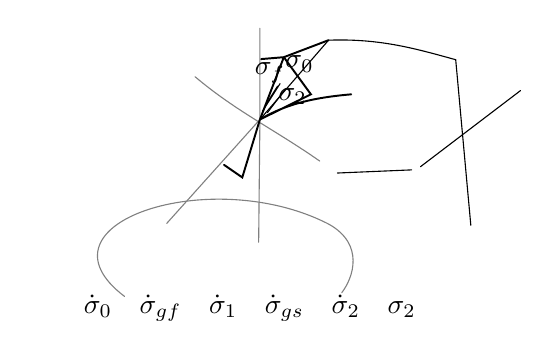
\begin{tikzpicture}[x=.008cm,y=-.008cm,line cap=round]
\draw[gray] (420,490)--(568,325)--(568,180) (568,325)--(566,520) (465,257)..controls(530,312)and(590,340)..(663,391);
\draw (568,325)--(677,199)..controls(760,196)and(817,213)..(879,230)--(903,493) (823,400)--(982,279) (691,410)--(809,405);
\draw[line width=.7pt] (511,397)--(540,417)--(568,325)--(606,226)--(677,199) (568,325)--(649,285)--(606,226)--(570,229) (568,325)..controls(610,300)and(655,290)..(713,285);
\draw (572,312)--(600,268) (580,314)--(609,276) (579,299)--(596,272);
\node at (584,251) {$\sigma_f$};\node at (631,237) {$\sigma_0$};\node at (620,288) {$\sigma_2$};
\draw[gray] (353,606)..controls(200,490)and(490,395)..(677,491)..controls(735,523)and(716,577)..(698,600);
\node[anchor=north] at (552,588) {$\dot\sigma_0\quad\dot\sigma_{\deleted{\unsure{g}}\inserted{f}}\quad\dot\sigma_1\quad\dot\sigma_{\deleted{\unsure{g}}\inserted{s}}\quad\dot\sigma_2\quad\deleted{\unsure{\sigma_2}}$};
\end{tikzpicture}}
\figure{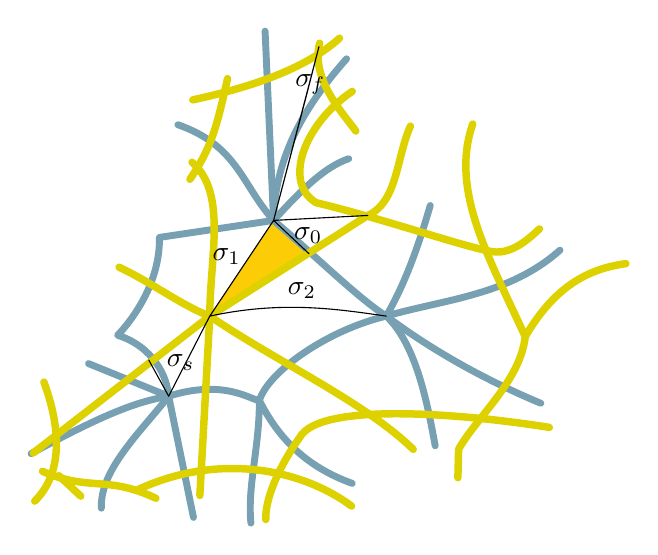
\begin{tikzpicture}[x=.009cm,y=-.009cm,line cap=round,line join=round]
\fill[yellow!65!orange] (1240,525)--(1330,390)--(1380,437)--cycle;
\draw[cyan!35!gray,line width=2.5pt] (1318,123)--(1330,390)..controls(1400,450)and(1450,500)..(1489,525)..controls(1530,564)and(1546,642)..(1558,708);
\draw[cyan!35!gray,line width=2.5pt] (1195,255)..controls(1280,285)and(1285,340)..(1330,390)..controls(1332,294)and(1380,222)..(1433,162);
\draw[cyan!35!gray,line width=2.5pt] (1330,390)..controls(1370,346)and(1403,314)..(1436,303);
\draw[cyan!35!gray,line width=2.5pt] (1330,390)--(1169,414)..controls(1170,478)and(1131,530)..(1110,552)..controls(1160,568)and(1180,610)..(1182,638)--(1217,809);
\draw[cyan!35!gray,line width=2.5pt] (988,719)..controls(1100,658)and(1142,645)..(1182,638)..controls(1261,613)and(1299,644)..(1310,644)..controls(1310,712)and(1293,763)..(1298,817);
\draw[cyan!35!gray,line width=2.5pt] (1087,796)..controls(1085,742)and(1141,690)..(1182,638)--(1069,592);
\draw[cyan!35!gray,line width=2.5pt] (1489,525)..controls(1405,545)and(1322,604)..(1310,644)..controls(1337,698)and(1377,738)..(1441,761);
\draw[cyan!35!gray,line width=2.5pt] (1489,525)..controls(1518,475)and(1537,417)..(1551,369);
\draw[cyan!35!gray,line width=2.5pt] (1489,525)..controls(1572,501)and(1662,496)..(1734,432);
\draw[cyan!35!gray,line width=2.5pt] (1489,525)..controls(1557,576)and(1633,617)..(1707,648);
\draw[yellow!70!olive,line width=2.7pt] (1216,220)..controls(1298,202)and(1374,177)..(1423,133);
\draw[yellow!70!olive,line width=2.7pt] (1395,140)..controls(1382,192)and(1430,241)..(1446,264);
\draw[yellow!70!olive,line width=2.7pt] (1441,208)..controls(1374,253)and(1342,336)..(1390,365)..controls(1486,388)and(1594,426)..(1638,434)..controls(1667,439)and(1693,413)..(1705,402);
\draw[yellow!70!olive,line width=2.7pt] (1265,190)..controls(1249,263)and(1241,289)..(1212,332);
\draw[yellow!70!olive,line width=2.7pt] (1215,308)..controls(1265,351)and(1240,442)..(1240,525)--(1226,778);
\draw[yellow!70!olive,line width=2.7pt] (1611,254)..controls(1578,348)and(1635,444)..(1685,554)..controls(1727,482)and(1775,458)..(1827,451);
\draw[yellow!70!olive,line width=2.7pt] (1685,554)..controls(1678,617)and(1615,669)..(1591,713)--(1590,753);
\draw[yellow!70!olive,line width=2.7pt] (1523,257)..controls(1503,302)and(1505,364)..(1463,383)--(1240,525)--(991,718);
\draw[yellow!70!olive,line width=2.7pt] (1112,456)..controls(1157,477)and(1202,511)..(1240,525)..controls(1332,588)and(1460,647)..(1527,713);
\draw[yellow!70!olive,line width=2.7pt] (1719,682)..controls(1587,661)and(1394,647)..(1367,696)..controls(1335,741)and(1318,785)..(1319,812);
\draw[yellow!70!olive,line width=2.7pt] (1006,618)..controls(1030,683)and(1033,747)..(993,786);
\draw[yellow!70!olive,line width=2.7pt] (1004,744)..controls(1071,773)and(1094,749)..(1164,782);
\draw[yellow!70!olive,line width=2.7pt] (1136,771)..controls(1252,716)and(1370,741)..(1440,793);
\draw[yellow!70!olive,line width=2.7pt] (1027,750)--(1058,779);
\draw (1330,390)--(1394,145)--(1375,219)--(1330,390)--(1463,383) (1240,525)--(1330,390)--(1380,437) (1240,525)..controls(1342,503)and(1419,515)..(1489,525) (1240,525)--(1182,638)--(1154,587);
\node at (1382,198) {$\sigma_f$};\node at (1379,411) {$\sigma_0$};\node at (1264,441) {$\sigma_1$};\node at (1370,489) {$\sigma_2$};\node at (1199,590) {$\sigma_s$};
\end{tikzpicture}}
\figure{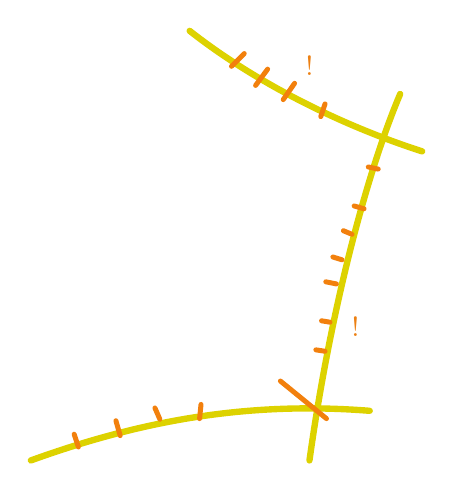
\begin{tikzpicture}[x=.009cm,y=-.009cm,line cap=round]
\draw[yellow!70!olive,line width=2.3pt] (2321,61)..controls(2415,135)and(2537,195)..(2649,231) (2618,150)..controls(2572,258)and(2520,452)..(2490,667) (2097,667)..controls(2260,608)and(2410,584)..(2575,597);
\draw[orange!80!brown,line width=1.8pt] (2380,111)--(2398,93) (2414,138)--(2431,115) (2453,158)--(2469,135) (2506,182)--(2512,164) (2573,253)--(2587,256) (2553,308)--(2567,312) (2538,343)--(2550,348) (2523,380)--(2536,384) (2513,415)--(2528,418) (2507,470)--(2519,472) (2499,511)--(2512,513) (2449,555)--(2514,608) (2158,630)--(2164,648) (2217,611)--(2223,632) (2272,593)--(2279,609) (2337,588)--(2335,608);
\node[text=orange!70!brown] at (2490,111) {$\unsure{!}$};\node[text=orange!70!brown] at (2555,479) {$!$};
\end{tikzpicture}}

Une carte dont les sommets
\uline{et} les faces sont d'ordre
pair, donne naissance à
une suite circulaire de
cinq involutions $2$ à $2$
commutantes
\[
\sigma_0\ \sigma_f\ \sigma_1\ \sigma_s\ \sigma_2\ [\sigma_0\ldots]
\]
donc à une carte pentagonale
\unsure{foncière|pondérée}, dont tous les
sommets sont d'ordre
deux ou quatre. Je n'arrive
pas bien à visualiser cette
dernière carte en termes de
la carte initiale....
\figure{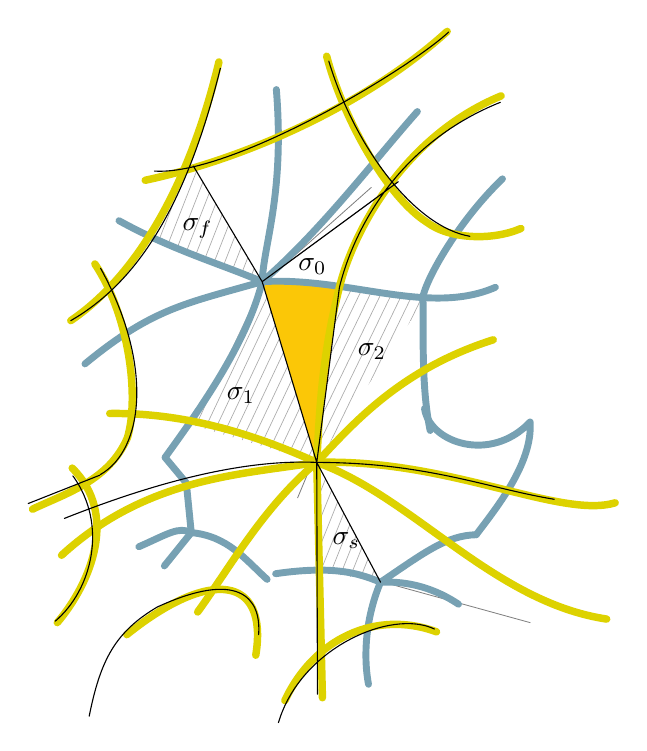
\begin{tikzpicture}[x=.009cm,y=-.009cm,line cap=round,line join=round]
\fill[yellow!60!orange] (1608,1143)--(1717,1151)--(1685,1398)--cycle;
\begin{scope}\clip (1511,980)--(1608,1143)--(1454,1086)--cycle;\foreach \k in {1410,1425,...,1635}\draw[gray!65,line width=.25pt](\k,1180)--++(90,-230);\end{scope}
\begin{scope}\clip (1608,1143)--(1505,1344)--(1685,1398)--cycle;\foreach \k in {1425,1440,...,1710}\draw[gray!65,line width=.25pt](\k,1440)--++(170,-360);\end{scope}
\begin{scope}\clip (1717,1151)--(1835,1172)--(1685,1398)--cycle;\foreach \k in {1580,1595,...,1865}\draw[gray!65,line width=.25pt](\k,1440)--++(160,-330);\end{scope}
\begin{scope}\clip (1685,1398)--(1775,1567)--(1685,1551)--cycle;\foreach \k in {1630,1645,...,1800}\draw[gray!65,line width=.25pt](\k,1590)--++(80,-200);\end{scope}
\draw[gray,line width=.3pt] (1608,1143)--(1800,1002) (1610,1145)--(1762,1010) (1678,1400)--(1658,1448) (1768,1564)--(1986,1624);
\draw[cyan!35!gray,line width=2.5pt] (1628,872)..controls(1640,1020)and(1610,1090)..(1608,1143)..controls(1586,1232)and(1515,1330)..(1471,1391)--(1501,1427)--(1508,1497)--(1470,1544);
\draw[cyan!35!gray,line width=2.5pt] (1358,1259)..controls(1454,1180)and(1500,1174)..(1608,1143)..controls(1691,1071)and(1766,972)..(1827,903);
\draw[cyan!35!gray,line width=2.5pt] (1406,1057)..controls(1480,1098)and(1552,1119)..(1608,1143)..controls(1730,1136)and(1843,1192)..(1937,1151);
\draw[cyan!35!gray,line width=2.5pt] (1947,998)..controls(1877,1065)and(1828,1160)..(1835,1172)..controls(1835,1238)and(1834,1300)..(1845,1353);
\draw[cyan!35!gray,line width=2.5pt] (1837,1322)..controls(1844,1370)and(1930,1400)..(1986,1341)..controls(1990,1400)and(1936,1465)..(1910,1500);
\draw[cyan!35!gray,line width=2.5pt] (1434,1517)..controls(1475,1499)and(1490,1488)..(1508,1497)..controls(1560,1502)and(1584,1535)..(1615,1563);
\draw[cyan!35!gray,line width=2.5pt] (1627,1555)..controls(1715,1542)and(1750,1557)..(1775,1567)..controls(1837,1525)and(1868,1501)..(1910,1500);
\draw[cyan!35!gray,line width=2.5pt] (1775,1567)..controls(1815,1565)and(1852,1576)..(1885,1598) (1775,1567)..controls(1755,1614)and(1750,1668)..(1758,1711);
\draw[yellow!70!olive,line width=2.7pt] (1547,833)..controls(1500,1029)and(1418,1144)..(1338,1198);
\draw[yellow!70!olive,line width=2.7pt] (1443,1000)..controls(1592,968)and(1759,890)..(1869,790);
\draw[yellow!70!olive,line width=2.7pt] (1699,825)..controls(1723,915)and(1785,1024)..(1840,1059)..controls(1873,1084)and(1934,1085)..(1973,1068);
\draw[yellow!70!olive,line width=2.7pt] (1945,881)..controls(1800,941)and(1733,1084)..(1717,1151)..controls(1692,1249)and(1689,1324)..(1685,1398)--(1693,1730);
\draw[yellow!70!olive,line width=2.7pt] (1372,1118)..controls(1420,1190)and(1435,1305)..(1418,1363)..controls(1392,1424)and(1330,1442)..(1284,1464);
\draw[yellow!70!olive,line width=2.7pt] (1393,1329)..controls(1518,1327)and(1627,1372)..(1685,1398)..controls(1820,1446)and(1934,1595)..(2094,1619);
\draw[yellow!70!olive,line width=2.7pt] (1325,1529)..controls(1445,1419)and(1580,1415)..(1685,1398)..controls(1870,1392)and(2028,1478)..(2106,1455);
\draw[yellow!70!olive,line width=2.7pt] (1934,1225)..controls(1805,1266)and(1738,1341)..(1685,1398)..controls(1610,1460)and(1560,1550)..(1517,1609);
\draw[yellow!70!olive,line width=2.7pt] (1340,1406)..controls(1405,1470)and(1368,1566)..(1319,1624);
\draw[yellow!70!olive,line width=2.7pt] (1417,1641)..controls(1535,1546)and(1617,1558)..(1599,1670);
\draw[yellow!70!olive,line width=2.7pt] (1640,1734)..controls(1680,1648)and(1767,1605)..(1854,1637);
\draw[line width=.4pt] (1549,842)..controls(1500,1040)and(1430,1145)..(1338,1198) (1456,987)..controls(1563,994)and(1810,847)..(1871,791) (1702,832)..controls(1740,957)and(1825,1066)..(1901,1079) (1944,890)..controls(1792,951)and(1734,1081)..(1717,1151)--(1685,1398)--(1686,1725) (1511,980)--(1608,1143)--(1685,1398)--(1775,1567) (1608,1143)--(1800,1002) (1329,1477)..controls(1450,1429)and(1577,1393)..(1685,1398)..controls(1840,1398)and(1928,1435)..(2020,1450) (1380,1124)..controls(1455,1260)and(1441,1380)..(1380,1415) (1278,1456)--(1379,1416) (1341,1417)..controls(1391,1486)and(1368,1578)..(1316,1622) (1364,1756)..controls(1380,1676)and(1401,1637)..(1460,1602) (1460,1602)..controls(1573,1550)and(1607,1587)..(1603,1641) (1631,1765)..controls(1662,1660)and(1790,1604)..(1851,1633);
\node at (1517,1068) {$\sigma_f$};\node at (1679,1122) {$\sigma_0$};\node at (1578,1304) {$\sigma_1$};\node at (1763,1242) {$\sigma_2$};\node at (1727,1508) {$\sigma_s$};
\end{tikzpicture}}
\figure{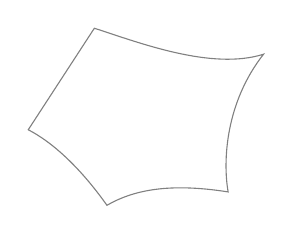
\begin{tikzpicture}[x=.01cm,y=-.01cm]
\draw[gray] (2374,817)..controls(2430,835)and(2523,871)..(2589,850)..controls(2541,911)and(2537,985)..(2544,1025)..controls(2468,1013)and(2423,1023)..(2390,1042)..controls(2356,994)and(2321,962)..(2290,946)--cycle;
\end{tikzpicture}}
\margin{\[\overbrace{\unsure{\tau_s|\sigma_s}\quad\unsure{\tau_a|\sigma_a}}\quad\unsure{\tau_r|\sigma_r}\qquad\unsure{\tau_{\deleted{\unsure{ver}}t}|\sigma_t}\]}
\figure{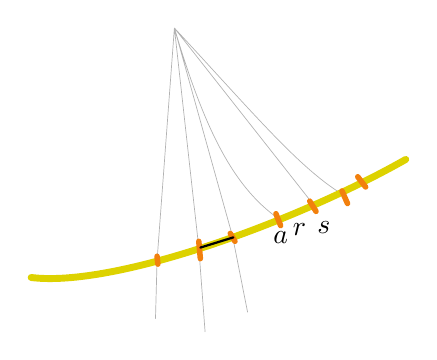
\begin{tikzpicture}[x=.01cm,y=-.01cm,line cap=round]
\draw[gray!60,line width=.25pt] (2457,1114)--(2435,1409)--(2433,1483) (2457,1114)--(2488,1393)--(2496,1500) (2457,1114)--(2531,1379)--(2550,1475) (2457,1114)..controls(2493,1235)and(2529,1314)..(2589,1356) (2457,1114)--(2635,1340) (2457,1114)..controls(2560,1225)and(2618,1295)..(2675,1328);
\draw[yellow!70!olive,line width=2.5pt] (2275,1431)..controls(2380,1444)and(2610,1361)..(2751,1281);
\draw[orange!80!brown,line width=2pt] (2435,1404)--(2436,1414) (2488,1385)--(2490,1407) (2528,1375)--(2534,1385) (2586,1350)--(2592,1365) (2629,1334)--(2637,1347) (2670,1321)--(2677,1337) (2690,1303)--(2700,1316);
\draw[line width=.8pt] (2490,1393)--(2532,1380);
\node at (2592,1380) {$a$};\node at (2616,1370) {$r$};\node at (2647,1368) {$s$};
\end{tikzpicture}}
\margin{94}
\scanpage{96}
\texttt{//* CRAY2 0439 I}
\begin{verbatim}
           00000000      00000000      00000000      00000000
         0000000000    0000000000    0000000000    0000000000
       00      0000  00      0000  00      0000  00      0000
      00     00 00  00     00 00  00     00 00  00     00 00
     00    00  00  00    00  00  00    00  00  00    00  00
    00   00   00  00   00   00  00   00   00  00   00   00
   00  00    00  00  00    00  00  00    00  00  00    00
  00 00     00  00 00     00  00 00     00  00 00     00
 0000      00  0000      00  0000      00  0000      00
000       00  000       00  000       00  000       00
0000000000    0000000000    0000000000    0000000000
00000000      00000000      00000000      00000000
\end{verbatim}
\figure{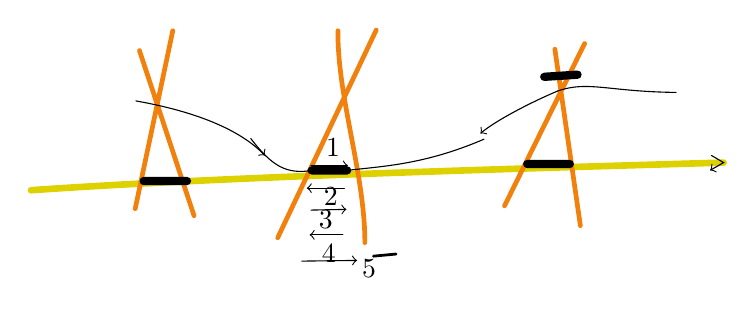
\begin{tikzpicture}[x=.009cm,y=-.009cm,line cap=round]
\draw[yellow!70!olive,line width=2.4pt] (1510,514)..controls(1780,495)and(2180,484)..(2487,475);
\draw[->] (2470,465)--(2487,475)--(2468,486);
\draw[orange!80!brown,line width=1.7pt] (1663,317)--(1740,550) (1710,289)--(1657,540) (1943,289)..controls(1942,382)and(1981,491)..(1981,588) (1997,288)--(1858,581) (2249,315)--(2285,564) (2291,307)--(2178,536);
\draw[line width=3pt] (1669,501)--(1730,501) (1906,486)--(1956,486) (2210,477)--(2270,477) (2234,354)--(2281,351);
\draw[->] (1658,388)..controls(1765,407)and(1815,439)..(1840,465);
\draw (1820,441)..controls(1850,480)and(1870,492)..(1907,486);
\draw (2420,376)..controls(2324,375)and(2296,359)..(2253,374);
\draw[->] (2253,374)..controls(2215,390)and(2165,416)..(2144,434);
\draw (2149,442)..controls(2065,478)and(2007,480)..(1956,486);
\draw[->] (1905,479)--(1957,479);\draw[->] (1952,511)--(1899,511);\draw[->] (1905,542)--(1955,541);\draw[->] (1950,577)--(1903,577);\draw[->] (1892,614)--(1970,613);
\node at (1936,454) {$1$};\node at (1933,523) {$2$};\node at (1926,555) {$3$};\node at (1930,603) {$4$};\node at (1987,625) {$5$};\draw[line width=1pt] (1993,607)--(2025,604);
\end{tikzpicture}}

\begin{verbatim}
 CCCCCCCCCC   RRRRRRRRRRR    AAAAAAAAAA   YY        YY   2222222222
CCCCCCCCCCCC  RRRRRRRRRRRR  AAAAAAAAAAAA  YY        YY  222222222222
CC        CC  RR        RR  AA        AA   YY      YY   22        22
CC            RR        RR  AA        AA    YY    YY              22
CC            RR        RR  AA        AA     YY  YY               22
CC            RRRRRRRRRRRR  AAAAAAAAAAAA      YYYY               22
CC            RRRRRRRRRRR   AAAAAAAAAAAA       YY              22
CC            RR    RR      AA        AA       YY            22
CC            RR     RR     AA        AA       YY          22
CC        CC  RR      RR    AA        AA       YY        22
CCCCCCCCCCCC  RR       RR   AA        AA       YY       222222222222
 CCCCCCCCCC   RR        RR  AA        AA       YY       222222222222
\end{verbatim}
\figure{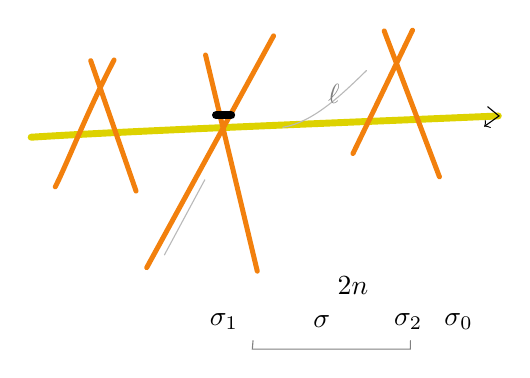
\begin{tikzpicture}[x=.009cm,y=-.009cm,line cap=round]
\draw[yellow!70!olive,line width=2.5pt] (2172,770)..controls(2330,760)and(2650,748)..(2831,740);
\draw[->] (2816,727)--(2832,740)--(2811,755);
\draw[orange!80!brown,line width=1.8pt] (2256,662)--(2320,846) (2289,661)..controls(2250,736)and(2222,809)..(2206,840) (2418,654)--(2491,959) (2514,627)--(2335,954) (2670,620)--(2748,826) (2710,619)--(2626,793);
\draw[gray!55] (2360,936)--(2417,830) (2527,756)..controls(2570,749)and(2610,710)..(2645,676);
\draw[line width=3pt] (2433,739)--(2454,739);
\node[text=gray] at (2599,709) {$\unsure{\ell}$};
\node at (2626,980) {$2n$};\node at (2444,1030) {$\sigma_1$};\node at (2582,1030) {$\sigma$};\node at (2704,1030) {$\sigma_2$};\node at (2775,1030) {$\sigma_0$};
\draw[gray] (2485,1057)--(2484,1069)--(2707,1069)--(2707,1057);
\end{tikzpicture}}

\begin{verbatim}
****A START JOB 439 CRAY2    ROOM    4.37.05 PM 16 AUG 82 R6.PR1    SYS JES2 JOB 439 START A****
****A START JOB 439 CRAY2    ROOM    4.37.05 PM 16 AUG 82 R6.PR1    SYS JES2 JOB 439 START A****
****A START JOB 439 CRAY2    ROOM    4.37.05 PM 16 AUG 82 R6.PR1    SYS JES2 JOB 439 START A****
****A START JOB 439 CRAY2    ROOM    4.37.05 PM 16 AUG 82 R6.PR1    SYS JES2 JOB 439 START A****
****A START JOB 439 CRAY2    ROOM    4.37.05 PM 16 AUG 82 R6.PR1    SYS JES2 JOB 439 START A****
****A START JOB 439 CRAY2    ROOM    4.37.05 PM 16 AUG 82 R6.PR1    SYS JES2 JOB 439 START A****
\end{verbatim}
\figure{
\begin{tikzpicture}[x=.25cm,y=.25cm]\draw[brown!70!black,line width=2pt] (0,0)--(2,3);\end{tikzpicture}}
\begin{verbatim}
DERNIERE MISE A JOUR DE JOURNAL : 11-08-82
ATTENTION ...........
        1. ARRET DE L'ORDINATEUR LE MARDI 17 AOUT DE 7 H A 8 H.
   ]    2. UNE MODIFICATION SYSTEME NOUS CONTRAINDRA A DETRUIRE
   ]       LE CONTENU DU DISQUE SPOOL LE MARDI 17 AOUT A 6 HEURES
   ]       VEUILLEZ RECUPERER VOS SORTIES EN ATTENTE AVANT CETTE
   ]       DATE. MERCI DE VOTRE COMPREHENSION.
   ]    3. UN ARRET EXCEPTIONNEL POUR PREPARER L'ARRIVEE DE NOUVELLES
   ]       UNITES AURA LIEU DU VENDREDI 20 AOUT A 17H 30 AU LUNDI
   ]       23 AOUT A 8H.
\end{verbatim}
\figure{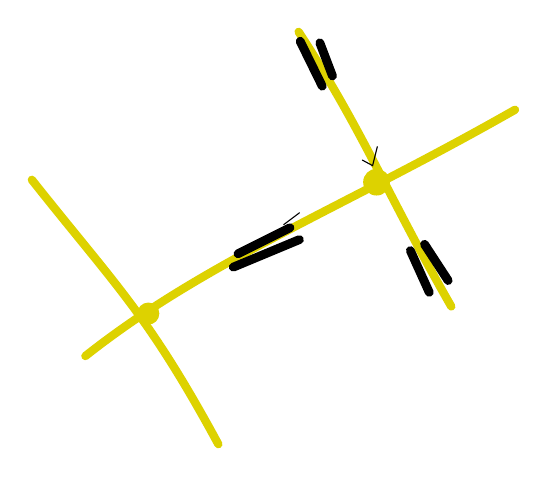
\begin{tikzpicture}[x=.01cm,y=-.01cm,line cap=round]
\draw[yellow!70!olive,line width=3pt] (1747,1776)..controls(1900,1655)and(2070,1590)..(2293,1463) (1679,1552)..controls(1786,1687)and(1826,1722)..(1916,1888) (2018,1364)..controls(2100,1490)and(2130,1570)..(2212,1713);
\fill[yellow!70!olive] (1827,1722) circle (14);\fill[yellow!70!olive] (2117,1555) circle (17);
\draw[black,line width=3.2pt] (2020,1376)--(2048,1433) (2045,1378)--(2061,1420) (1941,1646)--(2007,1613) (1935,1663)--(2019,1628) (2178,1634)--(2208,1680) (2160,1642)--(2184,1695);
\draw (2099,1527)--(2112,1534)--(2118,1510) (2019,1594)--(1999,1609);
\end{tikzpicture}}
\margin{95}
\scanpage{97}
\figure{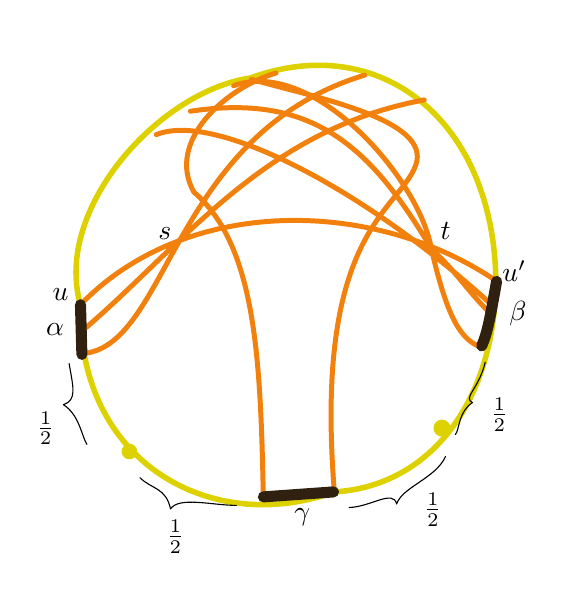
\begin{tikzpicture}[x=.009cm,y=-.009cm,line cap=round,line join=round]
\draw[yellow!70!olive,line width=2pt] (310,450)..controls(271,316)and(420,149)..(550,130)..controls(733,63)and(893,190)..(896,416)..controls(895,584)and(805,706)..(668,714)..controls(493,777)and(305,671)..(310,450);
\draw[orange!80!brown,line width=1.8pt] (310,450)..controls(457,297)and(722,298)..(896,416) (310,489)..controls(455,366)and(568,203)..(795,161) (310,519)..controls(435,514)and(436,209)..(711,126);
\draw[orange!80!brown,line width=1.8pt] (417,210)..controls(500,176)and(714,289)..(889,449) (465,177)..controls(637,151)and(719,226)..(805,371)..controls(839,402)and(855,429)..(886,460) (526,141)..controls(638,100)and(788,272)..(805,371)..controls(828,471)and(847,499)..(875,510);
\draw[orange!80!brown,line width=1.8pt] (586,123)..controls(514,144)and(430,220)..(470,291)..controls(558,367)and(564,528)..(568,723) (551,132)..controls(643,158)and(806,189)..(783,253)..controls(759,318)and(639,346)..(668,712);
\draw[black!75!brown,line width=4pt] (310,450)--(312,520) (897,417)..controls(888,468)and(884,490)..(876,508) (568,721)--(667,714);
\fill[yellow!70!olive] (379,657) circle (11);\fill[yellow!70!olive] (820,624) circle (12);
\draw (294,533)..controls(300,568)and(305,584)..(286,591)..controls(308,605)and(311,633)..(319,647);
\draw (394,694)..controls(410,710)and(431,708)..(437,738)..controls(449,720)and(496,733)..(530,733);
\draw (689,736)..controls(720,735)and(751,710)..(756,731)..controls(764,707)and(811,695)..(825,664);
\draw (881,531)..controls(872,569)and(849,581)..(863,588)..controls(843,601)and(845,625)..(839,633);
\node at (282,435) {$u$};\node at (274,485) {$\alpha$};\node at (429,349) {$s$};\node at (825,346) {$t$};\node at (922,402) {$u'$};\node at (927,463) {$\beta$};\node at (623,750) {$\unsure{\gamma}$};
\node at (261,624) {$\frac12$};\node at (444,777) {$\frac12$};\node at (807,739) {$\frac12$};\node at (901,605) {$\frac12$};
\end{tikzpicture}}
\figure{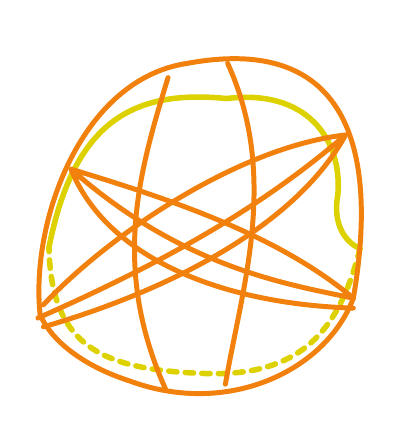
\begin{tikzpicture}[x=.014cm,y=-.014cm,line cap=round,line join=round]
\draw[yellow!70!olive,line width=2pt] (1058,263)..controls(1080,153)and(1130,119)..(1219,128)..controls(1292,119)and(1324,165)..(1320,215)..controls(1315,241)and(1326,258)..(1340,264);
\draw[yellow!70!olive,line width=2pt,dashed] (1340,264)..controls(1320,345)and(1280,382)..(1193,377)..controls(1100,373)and(1060,348)..(1058,263);
\draw[orange!80!brown,line width=1.8pt] (1050,324)..controls(1041,240)and(1087,110)..(1184,96)..controls(1348,66)and(1352,205)..(1334,309)..controls(1309,375)and(1220,417)..(1131,384)..controls(1085,369)and(1059,345)..(1050,324);
\draw[orange!80!brown,line width=1.8pt] (1166,109)..controls(1140,194)and(1114,281)..(1164,392) (1220,96)..controls(1267,199)and(1233,299)..(1218,387);
\draw[orange!80!brown,line width=1.8pt] (1053,315)..controls(1113,251)and(1230,172)..(1327,161) (1048,327)..controls(1177,270)and(1257,221)..(1327,161) (1053,335)..controls(1157,305)and(1279,248)..(1327,161);
\draw[orange!80!brown,line width=1.8pt] (1078,192)..controls(1174,221)and(1267,253)..(1334,309) (1078,192)..controls(1179,281)and(1272,296)..(1334,309) (1078,192)..controls(1110,271)and(1211,314)..(1334,318);
\end{tikzpicture}}
\figure{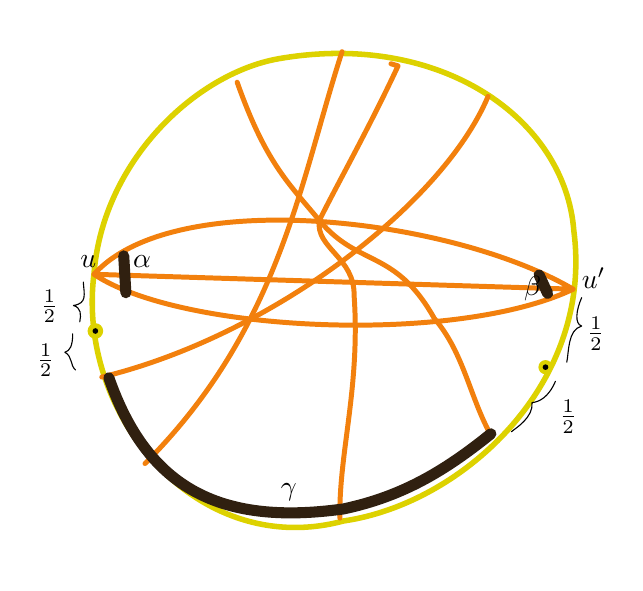
\begin{tikzpicture}[x=.009cm,y=-.009cm,line cap=round,line join=round]
\draw[yellow!70!olive,line width=2pt] (1588,459)..controls(1600,300)and(1731,176)..(1848,155)..controls(2076,115)and(2253,239)..(2265,398)..controls(2293,614)and(2107,783)..(1940,807)..controls(1735,862)and(1563,660)..(1588,459);
\draw[orange!80!brown,line width=1.8pt] (1588,459)..controls(1702,333)and(2092,379)..(2264,480) (1588,459)--(2264,480) (1588,459)..controls(1710,541)and(2098,559)..(2264,480);
\draw[orange!80!brown,line width=1.8pt] (1790,188)..controls(1830,301)and(1862,330)..(1906,383)..controls(1961,449)and(2013,423)..(2068,521)..controls(2110,570)and(2118,632)..(2148,686);
\draw[orange!80!brown,line width=1.8pt] (1938,145)..controls(1879,326)and(1851,535)..(1660,726);
\draw[orange!80!brown,line width=1.8pt] (2007,162)--(2017,165)..controls(1975,255)and(1929,336)..(1906,383)..controls(1900,422)and(1956,435)..(1955,489)..controls(1964,618)and(1933,713)..(1935,803);
\draw[orange!80!brown,line width=1.8pt] (2144,208)..controls(2080,360)and(1838,546)..(1599,604);
\draw[black!75!brown,line width=4pt] (1630,433)--(1633,485) (2216,460)--(2228,486) (1609,605)..controls(1662,756)and(1760,815)..(1940,790)..controls(2020,773)and(2080,739)..(2148,684);
\fill[yellow!70!olive] (1590,539) circle (11);\fill[black] (1590,539) circle (4);\fill[yellow!70!olive] (2225,590) circle (10);\fill[black] (2225,590) circle (4);
\draw (1573,470)..controls(1574,487)and(1579,500)..(1559,503)..controls(1570,506)and(1570,516)..(1568,526);
\draw (1558,543)..controls(1558,560)and(1554,567)..(1547,569)..controls(1558,575)and(1554,587)..(1562,594);
\draw (2276,492)..controls(2268,510)and(2266,529)..(2276,532)..controls(2256,537)and(2258,570)..(2255,583);
\draw (2239,610)..controls(2229,633)and(2216,639)..(2206,640)..controls(2208,661)and(2183,676)..(2177,681);
\node at (1580,441) {$u$};\node at (1656,441) {$\alpha$};\node at (2207,479) {$\unsure{\beta}$};\node at (2293,464) {$u'$};\node at (1863,767) {$\gamma$};
\node at (1525,504) {$\frac12$};\node at (1520,580) {$\frac12$};\node at (2296,543) {$\frac12$};\node at (2257,660) {$\frac12$};
\end{tikzpicture}}

\uline{NB} On suppose qu'il y a au moins une
ps dr qui ne passe pas par $s,t$ i.e.
qu'on n'est pas dans le cas $\mathrm{III}_{pq}$
($p,q\ge1$ — donc pas dans le cas $\unsure{\mathrm{St}_3|\mathfrak R_3}$ non plus)
Quand il n'y a qu'une seule ps. droite
qui ne passe pas $s,t$, \unsure{l'arc} de
spéc. exceptionnel $\unsure{\gamma}$ est de long. $0$.

On suppose qu'il y a une ps. droite
qui ne passe pas $\unsure{u},u'$, i.e. qu'on n'est
pas dans le cas trivial $\mathrm I_m$. Dans
le cas où il n'y en a qu'une,
l'arc de spécialisation \deleted{\unsure{de p.}} exceptionnel—
$\gamma$ est de \uline{longueur} $0$.
\figure{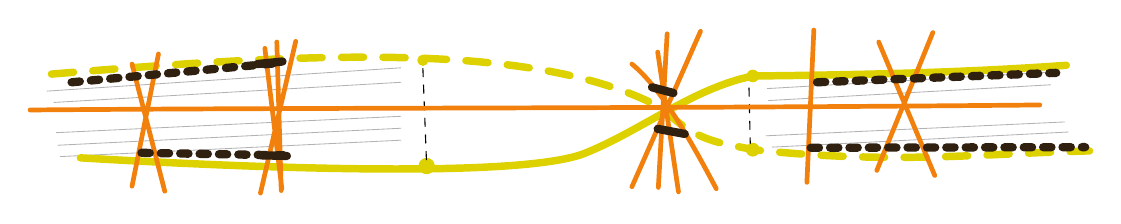
\begin{tikzpicture}[x=.008cm,y=-.008cm,line cap=round,line join=round]
\draw[gray!60,line width=.3pt] (174,1425)--(736,1388) (185,1443)--(736,1411) (189,1491)--(736,1465) (191,1511)--(736,1484) (195,1529)--(736,1503) (1318,1421)--(1767,1395) (1320,1440)--(1768,1415) (1316,1496)--(1790,1474) (1326,1514)--(1796,1490);
\draw[yellow!70!olive,line width=2.7pt,dash pattern=on 8pt off 7pt] (181,1398)..controls(588,1364)and(955,1344)..(1154,1454)..controls(1206,1508)and(1252,1508)..(1295,1518)..controls(1520,1542)and(1660,1524)..(1830,1520);
\draw[yellow!70!olive,line width=2.7pt] (227,1531)..controls(530,1549)and(922,1562)..(1025,1525)..controls(1115,1490)and(1198,1421)..(1295,1401)..controls(1487,1399)and(1640,1395)..(1793,1384);
\fill[yellow!70!olive] (777,1544) circle (13);\fill[yellow!70!olive] (771,1376) circle (9);\fill[yellow!70!olive] (1295,1518) circle (11);\fill[yellow!70!olive] (1295,1401) circle (10);
\draw[dashed] (771,1389)--(777,1544) (1289,1420)--(1291,1508);
\draw[orange!80!brown,line width=1.7pt] (147,1455)..controls(615,1451)and(1130,1453)..(1751,1447);
\draw[orange!80!brown,line width=1.7pt] (309,1382)--(361,1584) (351,1366)--(309,1576) (520,1357)--(547,1580) (539,1347)--(546,1583) (569,1346)--(513,1587) (1103,1382)..controls(1150,1420)and(1200,1510)..(1237,1580) (1144,1363)--(1177,1585) (1159,1334)--(1145,1578) (1212,1330)--(1103,1577) (1392,1328)--(1381,1570) (1495,1347)--(1584,1559) (1581,1332)--(1492,1551);
\draw[black!75!brown,line width=3pt,dash pattern=on 3pt off 4pt] (213,1411)--(535,1381) (324,1523)--(550,1527) (1397,1411)--(1777,1396) (1387,1515)--(1823,1514);
\draw[black!75!brown,line width=3pt] (508,1382)--(548,1378) (514,1527)--(555,1528) (1135,1419)--(1169,1428) (1144,1485)--(1187,1493);
\end{tikzpicture}}
\figure{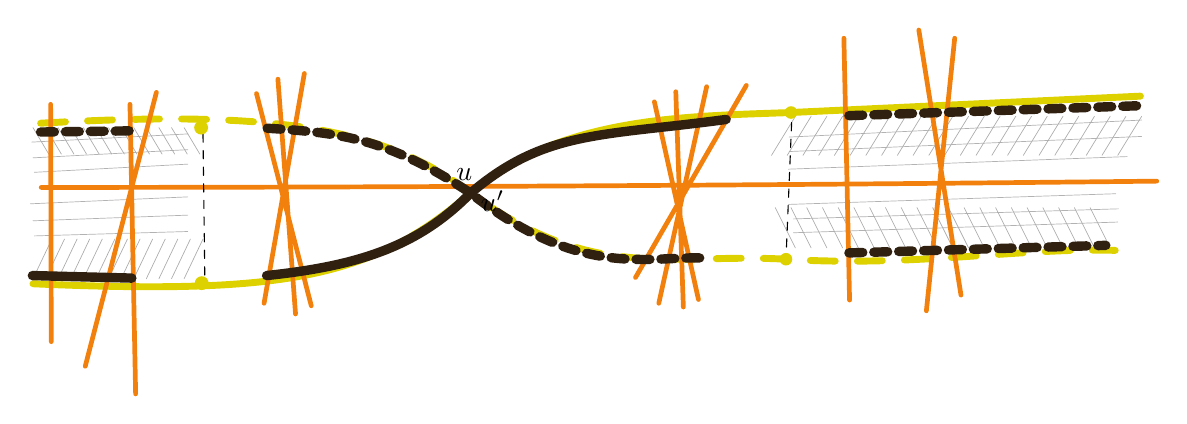
\begin{tikzpicture}[x=.008cm,y=-.008cm,line cap=round,line join=round]
\draw[gray!60,line width=.25pt] (82,1768)--(330,1755) (84,1793)--(330,1780) (86,1816)--(330,1803) (80,1866)--(330,1855) (84,1893)--(330,1884) (86,1917)--(330,1910) (1285,1760)--(1845,1733) (1285,1783)--(1845,1759) (1284,1811)--(1822,1791) (1284,1867)--(1804,1850) (1292,1890)--(1808,1874) (1292,1912)--(1807,1895);
\foreach \x in {84,104,...,324}\draw[gray!65,line width=.25pt] (\x,1745)--++(25,42);
\foreach \x in {84,104,...,324}\draw[gray!65,line width=.25pt] (\x,1985)--++(30,-63);
\foreach \x in {1295,1320,...,1845}\draw[gray!65,line width=.25pt] (\x,1727)--++(-38,62);
\foreach \x in {1295,1320,...,1800}\draw[gray!65,line width=.25pt] (\x,1936)--++(-32,-64);
\draw[yellow!70!olive,line width=2.5pt,dash pattern=on 9pt off 8pt] (96,1738)..controls(430,1719)and(634,1735)..(779,1849)..controls(974,1992)and(1095,1944)..(1280,1954)..controls(1480,1967)and(1660,1935)..(1803,1940);
\draw[yellow!70!olive,line width=2.5pt] (84,1993)..controls(494,2011)and(625,1981)..(779,1849)..controls(918,1727)and(1123,1727)..(1288,1721)--(1843,1695);
\draw[orange!80!brown,line width=1.7pt] (97,1840)..controls(605,1840)and(1230,1837)..(1869,1830);
\draw[orange!80!brown,line width=1.7pt] (112,1708)--(113,2085) (238,1708)--(247,2168) (280,1689)--(167,2124) (439,1691)--(526,2028) (473,1668)--(501,2041) (515,1659)--(451,2024) (1071,1704)--(1141,2018) (1105,1688)--(1117,2030) (1154,1680)--(1078,2024) (1217,1678)--(1041,1983) (1372,1603)--(1381,2019) (1491,1590)--(1558,2011) (1548,1603)--(1503,2036);
\draw[black!75!brown,line width=3.4pt,dash pattern=on 5pt off 4pt] (96,1752)--(249,1750) (456,1746)..controls(575,1753)and(649,1763)..(779,1849)..controls(951,1984)and(1057,1950)..(1143,1952) (1380,1726)--(1847,1710) (1380,1944)--(1788,1932);
\draw[black!75!brown,line width=3.4pt] (83,1980)--(241,1984) (455,1980)..controls(596,1965)and(694,1936)..(779,1849)..controls(897,1749)and(985,1759)..(1185,1732);
\draw[dashed] (354,1755)--(357,1991) (1289,1737)--(1280,1954);
\fill[yellow!70!olive] (351,1745) circle (11);\fill[yellow!70!olive] (352,1992) circle (11);\fill[yellow!70!olive] (1288,1721) circle (10);\fill[yellow!70!olive] (1280,1954) circle (10);
\node at (769,1820) {$u$};\node at (814,1862) {$u'$};
\end{tikzpicture}}
\margin{96}
\scanpage{98}
\texttt{//* CRAY2 0424 I}
\begin{verbatim}
           00000000      00000000      00000000      00000000
         0000000000    0000000000    0000000000    0000000000
       00      0000  00      0000  00      0000  00      0000
      00     00 00  00     00 00  00     00 00  00     00 00
     00    00  00  00    00  00  00    00  00  00    00  00
    00   00   00  00   00   00  00   00   00  00   00   00
   00  00    00  00  00    00  00  00    00  00  00    00
  00 00     00  00 00     00  00 00     00  00 00     00
 0000      00  0000      00  0000      00  0000      00
000       00  000       00  000       00  000       00
0000000000    0000000000    0000000000    0000000000
00000000      00000000      00000000      00000000
\end{verbatim}
\begin{verbatim}
 CCCCCCCCCC   RRRRRRRRRRR    AAAAAAAAAA   YY        YY   2222222222
CCCCCCCCCCCC  RRRRRRRRRRRR  AAAAAAAAAAAA  YY        YY  222222222222
CC        CC  RR        RR  AA        AA   YY      YY   22        22
CC            RR        RR  AA        AA    YY    YY              22
CC            RR        RR  AA        AA     YY  YY               22
CC            RRRRRRRRRRRR  AAAAAAAAAAAA      YYYY               22
CC            RRRRRRRRRRR   AAAAAAAAAAAA       YY              22
CC            RR    RR      AA        AA       YY            22
CC            RR     RR     AA        AA       YY          22
CC        CC  RR      RR    AA        AA       YY        22
CCCCCCCCCCCC  RR       RR   AA        AA       YY       222222222222
 CCCCCCCCCC   RR        RR  AA        AA       YY       222222222222
\end{verbatim}
\figure{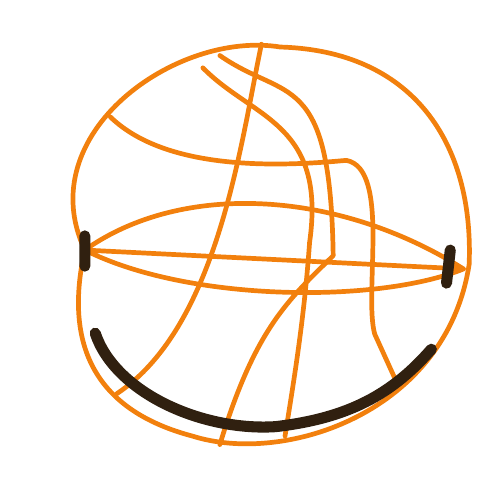
\begin{tikzpicture}[x=.012cm,y=-.012cm,line cap=round,line join=round]
\draw[orange!80!brown,line width=1.7pt] (2168,788)..controls(2110,665)and(2265,555)..(2375,573)..controls(2515,577)and(2580,674)..(2575,803)..controls(2551,960)and(2380,1016)..(2282,985)..controls(2180,958)and(2145,890)..(2168,788);
\draw[orange!80!brown,line width=1.7pt] (2168,788)..controls(2271,715)and(2436,724)..(2569,808) (2168,788)--(2569,808) (2168,788)..controls(2277,843)and(2478,845)..(2569,808);
\draw[orange!80!brown,line width=1.7pt] (2355,570)..controls(2333,675)and(2309,869)..(2202,940) (2293,595)..controls(2346,649)and(2424,653)..(2406,780)..controls(2400,865)and(2388,934)..(2380,985) (2311,582)..controls(2381,631)and(2428,595)..(2431,794)..controls(2383,841)and(2348,872)..(2311,994) (2195,647)..controls(2256,706)and(2380,699)..(2445,693)..controls(2492,702)and(2463,834)..(2475,877)--(2500,932);
\draw[black!75!brown,line width=4pt] (2168,773)--(2168,805) (2555,788)--(2551,823) (2179,876)..controls(2200,939)and(2292,980)..(2370,975)..controls(2448,966)and(2494,940)..(2535,893);
\end{tikzpicture}}

\begin{verbatim}
****A END JOB 424 CRAY2    ROOM    4.26.52 PM 16 AUG 82 R6.PR1    SYS JES2 JOB 424 END A****
****A END JOB 424 CRAY2    ROOM    4.26.52 PM 16 AUG 82 R6.PR1    SYS JES2 JOB 424 END A****
****A END JOB 424 CRAY2    ROOM    4.26.52 PM 16 AUG 82 R6.PR1    SYS JES2 JOB 424 END A****
****A END JOB 424 CRAY2    ROOM    4.26.52 PM 16 AUG 82 R6.PR1    SYS JES2 JOB 424 END A****
****A END JOB 424 CRAY2    ROOM    4.26.52 PM 16 AUG 82 R6.PR1    SYS JES2 JOB 424 END A****
****A END JOB 424 CRAY2    ROOM    4.26.52 PM 16 AUG 82 R6.PR1    SYS JES2 JOB 424 END A****
\end{verbatim}
\figure{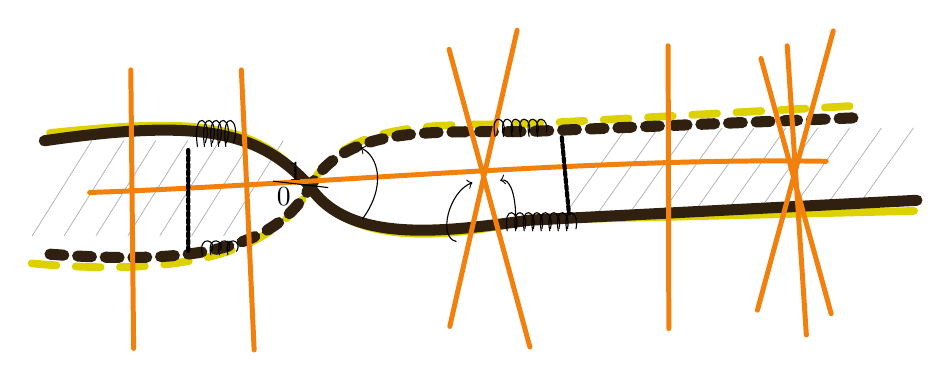
\begin{tikzpicture}[x=.009cm,y=-.009cm,line cap=round,line join=round]
\foreach \x in {630,675,...,915}\draw[gray!65,line width=.25pt] (\x,1642)--++(84,-134);
\foreach \x in {1385,1430,...,1815}\draw[gray!65,line width=.25pt] (\x,1607)--++(83,-117);
\draw[yellow!70!olive,line width=2.8pt] (655,1497)..controls(870,1475)and(949,1483)..(1022,1573)..controls(1082,1662)and(1224,1643)..(1332,1620)--(1874,1607);
\draw[yellow!70!olive,line width=2.8pt,dash pattern=on 9pt off 7pt] (629,1681)..controls(836,1700)and(972,1670)..(1022,1573)..controls(1076,1467)and(1235,1490)..(1353,1483)--(1804,1458);
\draw[black!75!brown,line width=4pt] (647,1508)..controls(868,1476)and(951,1494)..(1022,1573)..controls(1079,1658)and(1226,1634)..(1332,1620)--(1878,1592);
\draw[black!75!brown,line width=4pt,dash pattern=on 5pt off 5pt] (655,1668)..controls(848,1683)and(970,1665)..(1022,1573)..controls(1076,1476)and(1226,1500)..(1353,1494)--(1806,1475);
\draw[orange!80!brown,line width=1.8pt] (711,1581)..controls(1026,1570)and(1426,1531)..(1750,1537) (769,1408)--(773,1801) (925,1408)--(943,1803) (1218,1379)--(1332,1799) (1314,1352)--(1219,1770) (1527,1374)--(1528,1773) (1658,1392)--(1757,1752) (1695,1374)--(1722,1782) (1760,1353)--(1653,1747);
\draw[line width=1.5pt,densely dotted] (850,1521)--(850,1665) (1377,1503)--(1387,1610);
\draw (970,1565)--(1047,1574);\node at (985,1587) {$\unsure{0}$};\node at (1001,1552) {$\unsure{1}$};
\draw[->] (1096,1618)..controls(1130,1572)and(1118,1529)..(1093,1518);
\draw[->] (1228,1650)..controls(1202,1645)and(1217,1580)..(1251,1567);
\draw[->] (1312,1613)..controls(1311,1580)and(1303,1561)..(1290,1564);
\foreach \x in {863,873,...,903}\draw (\x,1516)..controls(\x-8,1460)and(\x+23,1476)..(\x+11,1511);
\foreach \x in {870,882,...,906}\draw (\x,1669)..controls(\x-7,1639)and(\x+23,1648)..(\x+12,1664);
\foreach \x in {1283,1295,...,1343}\draw (\x,1502)..controls(\x-8,1465)and(\x+18,1476)..(\x+12,1496);
\foreach \x in {1300,1312,...,1384}\draw (\x,1635)..controls(\x-7,1598)and(\x+19,1605)..(\x+13,1632);
\end{tikzpicture}}
\figure{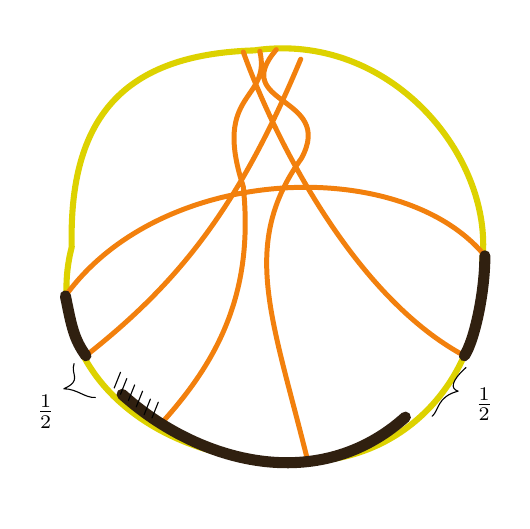
\begin{tikzpicture}[x=.01cm,y=-.01cm,line cap=round,line join=round]
\draw[yellow!70!olive,line width=2.2pt] (2118,1655)..controls(2114,1490)and(2184,1410)..(2350,1405)..controls(2522,1380)and(2653,1539)..(2640,1670)..controls(2643,1829)and(2536,1925)..(2418,1927)..controls(2230,1937)and(2077,1814)..(2118,1655);
\draw[orange!80!brown,line width=1.8pt] (2110,1717)..controls(2232,1548)and(2538,1538)..(2643,1666) (2136,1793)..controls(2254,1700)and(2330,1605)..(2409,1416) (2336,1407)..controls(2374,1513)and(2475,1717)..(2617,1793) (2357,1406)..controls(2372,1470)and(2296,1456)..(2336,1578)..controls(2350,1714)and(2303,1801)..(2230,1881) (2378,1404)..controls(2317,1475)and(2453,1462)..(2410,1542)..controls(2331,1652)and(2373,1745)..(2418,1927);
\draw[black!75!brown,line width=4pt] (2110,1717)..controls(2118,1757)and(2121,1772)..(2136,1793) (2643,1666)..controls(2643,1712)and(2630,1773)..(2617,1793) (2182,1842)..controls(2280,1930)and(2432,1970)..(2542,1871);
\foreach \x/\y in {2172/1834,2180/1842,2190/1850,2200/1858,2210/1868,2220/1872}\draw (\x,\y)--++(8,-20);
\draw (2121,1803)..controls(2116,1817)and(2132,1824)..(2108,1835)..controls(2125,1835)and(2135,1847)..(2148,1846);
\draw (2619,1808)..controls(2600,1825)and(2599,1835)..(2609,1838)..controls(2582,1845)and(2585,1862)..(2576,1870);
\node at (2085,1864) {$\frac12$};\node at (2642,1855) {$\frac12$};
\end{tikzpicture}}
\figure{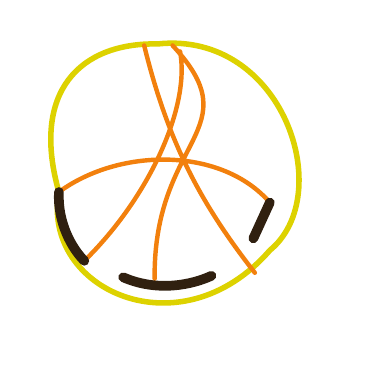
\begin{tikzpicture}[x=.019cm,y=-.019cm,line cap=round,line join=round]
\draw[yellow!70!olive,line width=2pt] (1829,2034)..controls(1810,1967)and(1843,1934)..(1895,1935)..controls(1979,1926)and(2015,2036)..(1970,2073)..controls(1910,2142)and(1817,2099)..(1829,2034);
\draw[orange!80!brown,line width=1.6pt] (1829,2034)..controls(1870,2004)and(1938,2004)..(1970,2041) (1846,2080)..controls(1889,2038)and(1917,1977)..(1910,1940) (1886,1936)..controls(1902,2001)and(1924,2042)..(1960,2088) (1905,1936)..controls(1958,1993)and(1892,1997)..(1893,2092);
\draw[black!75!brown,line width=3.5pt] (1829,2034)..controls(1828,2055)and(1838,2072)..(1846,2080) (1970,2041)--(1959,2065) (1872,2091)..controls(1895,2101)and(1918,2096)..(1931,2090);
\end{tikzpicture}}
\figure{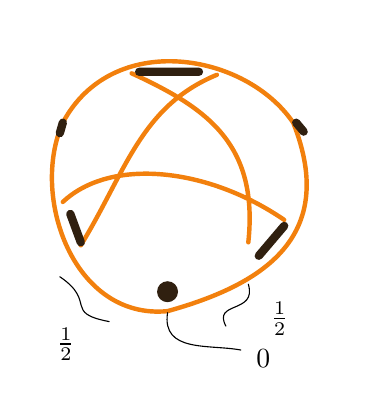
\begin{tikzpicture}[x=.019cm,y=-.019cm,line cap=round,line join=round]
\draw[orange!80!brown,line width=1.6pt] (2105,2009)..controls(2138,1947)and(2227,1962)..(2259,2009)..controls(2290,2087)and(2236,2118)..(2175,2135)..controls(2112,2141)and(2083,2058)..(2105,2009);
\draw[orange!80!brown,line width=1.6pt] (2105,2062)..controls(2137,2032)and(2202,2039)..(2253,2074) (2117,2091)..controls(2147,2042)and(2157,1998)..(2208,1977) (2151,1976)..controls(2201,1999)and(2236,2023)..(2229,2089);
\draw[black!75!brown,line width=3pt] (2105,2009)--(2103,2016) (2156,1975)--(2196,1975) (2261,2009)--(2266,2015) (2110,2070)--(2117,2089) (2253,2078)--(2236,2098);
\fill[black!75!brown] (2175,2122) circle (7);
\draw (2103,2112)..controls(2128,2129)and(2105,2136)..(2136,2142) (2229,2117)..controls(2235,2137)and(2205,2128)..(2214,2145) (2175,2136)..controls(2171,2163)and(2203,2157)..(2224,2161);
\node at (2107,2157) {$\frac12$};\node at (2250,2140) {$\frac12$};\node at (2239,2167) {$0$};
\end{tikzpicture}}
\margin{97}
\scanpage{100}
\texttt{//* CRAY2 0344 I}
\begin{verbatim}
           00000000      00000000    555555555555       11
         0000000000    0000000000   555555555555      111
       00      0000  00      0000  55               1111
      00     00 00  00     00 00  55                 11
     00    00  00  00    00  00  55                 11
    00   00   00  00   00   00  555555555          11
   00  00    00  00  00    00  5555555555         11
  00 00     00  00 00     00           55        11
 0000      00  0000      00            55       11
000       00  000       00            55       11
0000000000    0000000000   555555555555   1111111111
00000000      00000000    55555555555    1111111111
\end{verbatim}
\begin{verbatim}
 CCCCCCCCCC   RRRRRRRRRRR    AAAAAAAAAA   YY        YY   2222222222
CCCCCCCCCCCC  RRRRRRRRRRRR  AAAAAAAAAAAA  YY        YY  222222222222
CC        CC  RR        RR  AA        AA   YY      YY   22        22
CC            RR        RR  AA        AA    YY    YY              22
CC            RR        RR  AA        AA     YY  YY               22
CC            RRRRRRRRRRRR  AAAAAAAAAAAA      YYYY               22
CC            RRRRRRRRRRR   AAAAAAAAAAAA       YY              22
CC            RR    RR      AA        AA       YY            22
CC            RR     RR     AA        AA       YY          22
CC        CC  RR      RR    AA        AA       YY        22
CCCCCCCCCCCC  RR       RR   AA        AA       YY       222222222222
 CCCCCCCCCC   RR        RR  AA        AA       YY       222222222222
\end{verbatim}
\begin{verbatim}
****A END JOB 344 CRAY2    ROOM    3.08.54 PM 19 AUG 82 R6.PR1    SYS JES2 JOB 344 END A****
****A END JOB 344 CRAY2    ROOM    3.08.54 PM 19 AUG 82 R6.PR1    SYS JES2 JOB 344 END A****
****A END JOB 344 CRAY2    ROOM    3.08.54 PM 19 AUG 82 R6.PR1    SYS JES2 JOB 344 END A****
****A END JOB 344 CRAY2    ROOM    3.08.54 PM 19 AUG 82 R6.PR1    SYS JES2 JOB 344 END A****
****A END JOB 344 CRAY2    ROOM    3.08.54 PM 19 AUG 82 R6.PR1    SYS JES2 JOB 344 END A****
****A END JOB 344 CRAY2    ROOM    3.08.54 PM 19 AUG 82 R6.PR1    SYS JES2 JOB 344 END A****
\end{verbatim}
\figure{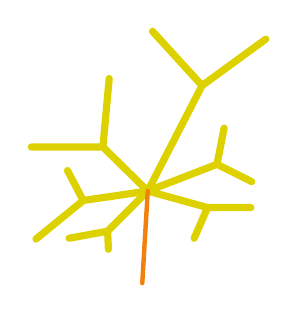
\begin{tikzpicture}[x=.01cm,y=-.01cm,line cap=round,line join=round]
\draw[yellow!70!olive,line width=2.6pt] (1968,1404)--(2028,1355)--(2110,1343)--(2179,1209)--(2260,1150) (2179,1209)--(2116,1140) (2110,1343)--(2053,1287)--(2061,1200) (2053,1287)--(1962,1287) (2028,1355)--(2008,1317) (2110,1343)--(2059,1394)--(2010,1403) (2059,1394)--(2060,1417) (2110,1343)--(2198,1309)--(2242,1331) (2198,1309)--(2207,1263) (2110,1343)--(2186,1364)--(2241,1364) (2186,1364)--(2169,1403);
\draw[orange!80!brown,line width=1.6pt] (2110,1343)--(2103,1460);
\end{tikzpicture}}
\figure{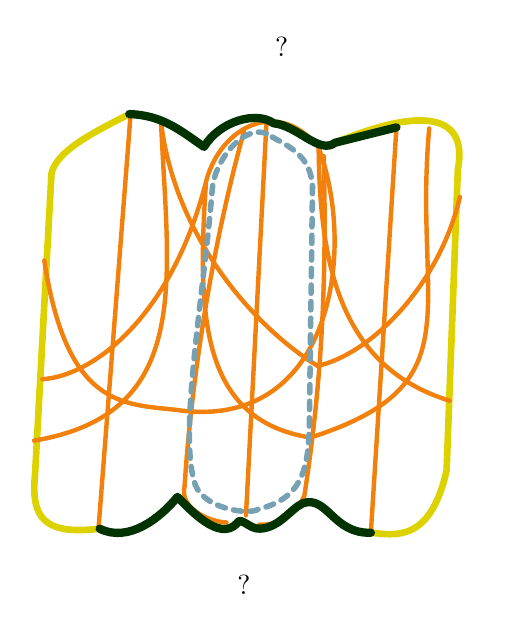
\begin{tikzpicture}[x=.013cm,y=-.013cm,line cap=round,line join=round]
\node at (1410,1390) {$?$};\node at (1373,1916) {$?$};
\draw[yellow!70!olive,line width=2.4pt] (1185,1514)..controls(1190,1491)and(1230,1472)..(1261,1456)..controls(1294,1457)and(1312,1473)..(1334,1488)..controls(1350,1462)and(1386,1453)..(1402,1465)..controls(1425,1467)and(1447,1496)..(1462,1484)..controls(1551,1447)and(1592,1458)..(1582,1510)--(1571,1804)..controls(1555,1876)and(1519,1867)..(1497,1865)..controls(1460,1866)and(1455,1829)..(1431,1836)..controls(1419,1841)and(1408,1860)..(1389,1861)..controls(1378,1862)and(1370,1848)..(1366,1856)..controls(1349,1874)and(1320,1842)..(1308,1830)..controls(1291,1851)and(1260,1875)..(1232,1861)..controls(1175,1868)and(1165,1848)..(1169,1807)--cycle;
\draw[orange!80!brown,line width=1.6pt] (1262,1460)--(1231,1860) (1292,1464)..controls(1299,1619)and(1324,1749)..(1168,1775) (1522,1469)--(1497,1865) (1554,1470)..controls(1538,1648)and(1600,1720)..(1438,1772)..controls(1331,1755)and(1327,1654)..(1336,1522) (1178,1599)..controls(1200,1743)and(1255,1739)..(1307,1745)..controls(1458,1767)and(1484,1591)..(1446,1489)..controls(1407,1439)and(1350,1468)..(1336,1522)..controls(1302,1655)and(1225,1712)..(1176,1715) (1292,1464)..controls(1306,1579)and(1386,1666)..(1445,1702)..controls(1495,1691)and(1563,1626)..(1584,1537) (1446,1489)..controls(1447,1601)and(1466,1703)..(1574,1736);
\draw[orange!80!brown,line width=1.6pt] (1395,1465)--(1375,1848) (1373,1473)..controls(1339,1596)and(1321,1726)..(1315,1820)..controls(1310,1840)and(1337,1854)..(1356,1855) (1451,1497)..controls(1454,1620)and(1449,1719)..(1432,1829)..controls(1421,1852)and(1402,1858)..(1388,1857);
\draw[cyan!35!gray,line width=2pt,dashed] (1395,1475)..controls(1373,1466)and(1344,1501)..(1342,1530)..controls(1334,1630)and(1310,1764)..(1324,1813)..controls(1329,1842)and(1379,1848)..(1387,1842)..controls(1431,1831)and(1437,1802)..(1437,1750)--(1440,1527)..controls(1438,1493)and(1412,1486)..(1395,1475);
\draw[black!80!green,line width=3pt] (1261,1456)..controls(1294,1457)and(1312,1473)..(1334,1488)..controls(1350,1462)and(1386,1453)..(1402,1465)..controls(1425,1467)and(1447,1496)..(1462,1484)--(1522,1469) (1232,1861)..controls(1260,1875)and(1291,1851)..(1308,1830)..controls(1320,1842)and(1349,1874)..(1366,1856)..controls(1370,1848)and(1378,1862)..(1389,1861)..controls(1408,1860)and(1419,1841)..(1431,1836)..controls(1455,1829)and(1460,1866)..(1497,1865);
\end{tikzpicture}}
\figure{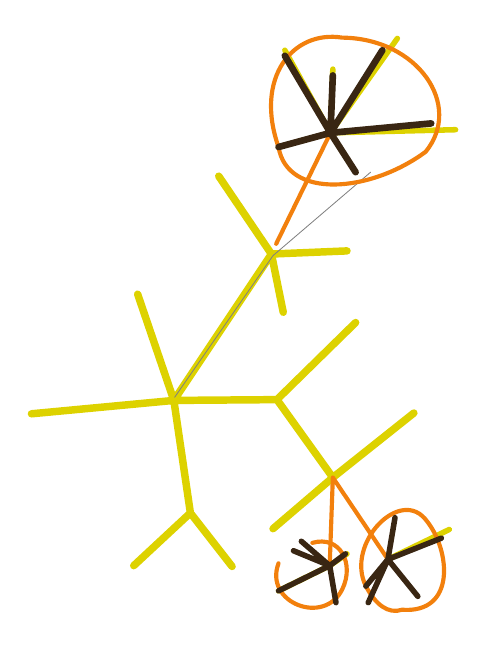
\begin{tikzpicture}[x=.01cm,y=-.01cm,line cap=round,line join=round]
\draw[yellow!70!olive,line width=2.7pt] (1649,1950)--(1830,1933)--(1954,1747)--(2050,1743) (1954,1747)--(1887,1648) (1954,1747)--(1969,1821) (1830,1933)--(1784,1798) (1830,1933)--(1851,2076)--(1779,2143) (1851,2076)--(1904,2144) (1830,1933)--(1961,1932)--(2061,1834) (1961,1932)--(2032,2031)--(2135,1949) (2032,2031)--(1956,2096);
\draw[gray,line width=.3pt] (1831,1929)--(1956,1749)--(2080,1643);
\draw[orange!80!brown,line width=1.5pt] (1960,1734)--(2029,1593) (2032,2031)--(2028,2143) (2032,2031)--(2102,2135);
\draw[yellow!70!olive,line width=2pt] (1963,1611)--(2029,1593)--(2188,1589) (2029,1593)--(1971,1488) (2029,1593)--(2114,1473) (2029,1593)--(2032,1512) (2029,1593)--(2061,1643);
\draw[orange!80!brown,line width=1.5pt] (1963,1611)..controls(1932,1523)and(1981,1462)..(2044,1472)..controls(2140,1473)and(2198,1558)..(2150,1617)..controls(2080,1669)and(1974,1678)..(1963,1611);
\draw[black!70!brown,line width=2.4pt] (1963,1611)--(2029,1593)--(2157,1581) (2029,1593)--(1971,1495) (2029,1593)--(2095,1488) (2029,1593)--(2032,1520) (2029,1593)--(2061,1643);
\draw[yellow!70!olive,line width=2pt] (1963,2175)--(2028,2143)--(2050,2128) (2102,2135)--(2180,2097);
\draw[orange!80!brown,line width=1.5pt] (1963,2140)..controls(1944,2190)and(2021,2220)..(2044,2173)..controls(2060,2140)and(2041,2104)..(2006,2114) (2074,2169)..controls(2047,2115)and(2119,2040)..(2152,2087)..controls(2181,2124)and(2189,2204)..(2120,2199)..controls(2102,2205)and(2086,2192)..(2074,2169);
\draw[black!70!brown,line width=2pt] (1963,2175)--(2028,2143)--(2048,2128) (2028,2143)--(1982,2124) (2028,2143)--(1992,2112) (2028,2143)--(2036,2190) (2074,2169)--(2102,2135)--(2170,2108) (2102,2135)--(2111,2082) (2102,2135)--(2077,2190) (2102,2135)--(2140,2182);
\end{tikzpicture}}
\figure{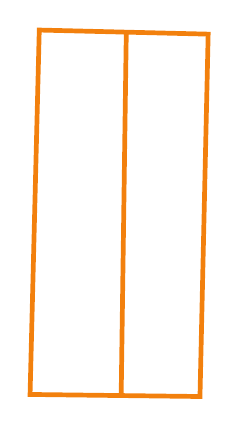
\begin{tikzpicture}[x=.013cm,y=-.013cm]\draw[orange!80!brown,line width=1.7pt] (2213,1569)--(2378,1573)--(2370,1927)--(2204,1925)--cycle (2298,1572)--(2293,1927);\end{tikzpicture}}
\margin{99}
\scanpage{101}
\figure{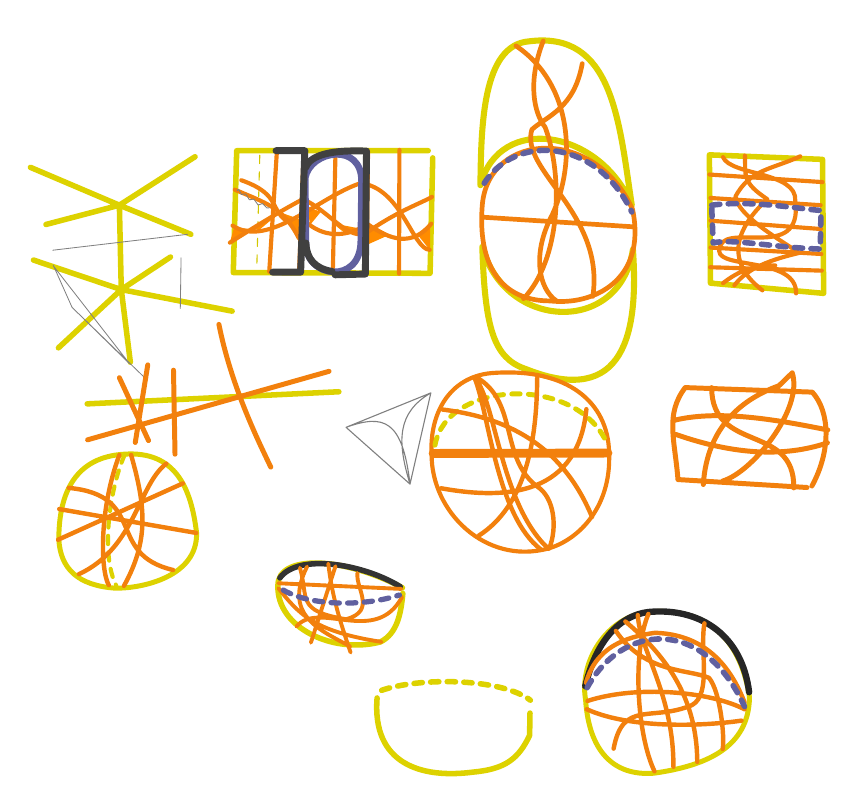
\begin{tikzpicture}[x=.0048cm,y=-.0048cm,line cap=round,line join=round]
\draw[yellow!70!olive,line width=2pt] (341,432)--(576,532)--(776,404) (382,583)--(576,532)--(765,609) (576,532)--(581,755)--(605,947) (349,677)--(581,755)--(874,812) (415,909)--(581,755)--(711,669);
\draw[gray,line width=.3pt] (400,651)--(756,609) (401,690)--(451,802)--(603,951)--(402,693) (451,802)--(641,986) (739,671)--(737,805);
\draw[yellow!70!olive,line width=2pt] (886,388)--(1392,388) (1404,407)--(1397,712)--(877,710)--(886,388);
\draw[yellow!60!olive,dashed] (947,400)--(939,701);
\fill[orange!90!yellow] (868,631)--(1001,551)--(946,597)--(879,591)--cycle (1001,551)--(1054,616)--(1058,571)--cycle (1080,584)--(1108,550)--(1072,535)--cycle (1140,580)--(1208,593)--(1172,606)--cycle (1210,619)--(1243,584)--(1290,610)--(1232,636)--cycle (1364,610)--(1397,578)--(1397,651)--cycle;
\draw[orange!80!brown,line width=1.5pt] (992,393)--(972,708) (1063,391)--(1051,707) (1147,395)--(1140,708) (1233,390)--(1229,713) (1316,386)--(1315,713);
\draw[orange!80!brown,line width=1.5pt] (881,491)..controls(965,527)and(1009,538)..(1050,619) (898,466)..controls(1009,505)and(968,547)..(1028,580) (868,631)..controls(964,570)and(1018,539)..(1061,516)..controls(1130,546)and(1184,632)..(1232,603)..controls(1310,548)and(1375,526)..(1402,510) (875,586)..controls(970,648)and(1103,510)..(1213,474)..controls(1321,485)and(1351,649)..(1396,650) (1066,573)..controls(1112,618)and(1175,619)..(1232,582)..controls(1292,625)and(1350,642)..(1400,581);
\draw[blue!25!gray,line width=2.4pt] (1067,460)..controls(1080,387)and(1218,363)..(1216,471)--(1214,627)..controls(1213,745)and(1068,723)..(1069,635)--cycle;
\draw[black!75,line width=2.5pt] (990,388)--(1066,388)--(1055,709)--(981,709) (1068,433)..controls(1084,389)and(1170,387)..(1229,389)--(1226,714)--(1146,716) (1069,632)..controls(1070,673)and(1093,700)..(1138,707);
\draw[gray,line width=.3pt] (887,494)..controls(895,480)and(895,513)..(903,503)..controls(914,493)and(916,527)..(925,517)..controls(934,505)and(940,542)..(948,530)..controls(956,518)and(963,547)..(972,539);
\draw[yellow!70!olive,line width=2.2pt] (1530,479)..controls(1532,323)and(1535,108)..(1659,99)..controls(1879,71)and(1896,306)..(1930,532) (1530,479)..controls(1580,288)and(1846,331)..(1930,532) (1535,642)..controls(1542,853)and(1563,936)..(1650,965)..controls(1914,1070)and(1948,865)..(1933,649) (1535,642)..controls(1594,863)and(1899,877)..(1933,649);
\draw[orange!80!brown,line width=1.7pt] (1535,531)..controls(1552,337)and(1832,322)..(1932,543)..controls(1971,731)and(1828,798)..(1714,785)..controls(1582,785)and(1522,687)..(1535,531) (1540,564)--(1932,589) (1624,111)..controls(1776,214)and(1783,420)..(1720,557)..controls(1665,661)and(1684,753)..(1731,785) (1696,98)..controls(1654,206)and(1671,288)..(1701,326)..controls(1750,457)and(1742,676)..(1644,779) (1799,158)..controls(1778,276)and(1708,295)..(1666,332)..controls(1633,441)and(1860,553)..(1827,773);
\draw[blue!25!gray,line width=2pt,dashed] (1540,474)..controls(1621,345)and(1834,351)..(1930,550);
\draw[yellow!70!olive,line width=2pt] (2135,399)--(2434,411)--(2437,765)--(2138,738)--cycle;
\draw[orange!80!brown,line width=1.5pt] (2135,451)--(2434,471) (2138,513)--(2429,532) (2138,573)--(2430,595) (2138,644)--(2431,661) (2137,696)--(2432,705) (2171,405)..controls(2191,454)and(2368,443)..(2362,521)..controls(2384,691)and(2160,564)..(2161,654)..controls(2164,700)and(2367,670)..(2364,765) (2229,401)..controls(2231,453)and(2220,471)..(2288,516)..controls(2232,569)and(2155,664)..(2275,757) (2375,403)..controls(2298,438)and(2243,437)..(2204,509)..controls(2208,556)and(2314,620)..(2373,658)..controls(2275,681)and(2230,706)..(2201,744) (2171,738)..controls(2234,689)and(2272,695)..(2309,691);
\draw[blue!25!gray,line width=2pt,dashed] (2141,532)..controls(2246,518)and(2374,542)..(2430,546)--(2428,648)..controls(2307,644)and(2189,619)..(2145,632)--cycle;
\draw[yellow!70!olive,line width=2pt] (491,1057)--(1156,1025);
\draw[orange!80!brown,line width=1.8pt] (492,1152)--(1130,971) (576,988)--(653,1154) (651,954)--(618,1159) (719,968)--(723,1190) (839,847)..controls(871,1007)and(939,1147)..(976,1224);
\draw[yellow!70!olive,line width=1.8pt] (416,1415)..controls(416,1290)and(461,1198)..(588,1190)..controls(726,1180)and(766,1282)..(780,1398)..controls(783,1513)and(638,1545)..(565,1544)..controls(467,1537)and(420,1493)..(416,1415);
\draw[yellow!70!olive,line width=1.5pt,dashed] (590,1192)..controls(553,1272)and(524,1452)..(568,1538);
\draw[orange!80!brown,line width=1.6pt] (442,1279)..controls(652,1299)and(538,1454)..(718,1496) (417,1335)--(779,1398) (414,1416)--(744,1267) (469,1507)..controls(618,1438)and(626,1271)..(700,1215) (576,1192)..controls(523,1333)and(525,1495)..(548,1536) (607,1192)..controls(646,1329)and(654,1419)..(588,1538);
\draw[gray,line width=.4pt] (1175,1119)--(1399,1028)--(1344,1269)--cycle (1175,1119)..controls(1275,1083)and(1324,1099)..(1344,1269) (1399,1028)..controls(1310,1080)and(1309,1155)..(1344,1269);
\draw[orange!80!brown,line width=1.5pt] (1401,1190)..controls(1395,1076)and(1454,980)..(1569,975)..controls(1760,963)and(1867,1052)..(1870,1185)..controls(1877,1340)and(1778,1422)..(1706,1440)..controls(1543,1482)and(1400,1342)..(1401,1190);
\draw[yellow!70!olive,line width=1.8pt,dashed] (1410,1166)..controls(1439,997)and(1779,977)..(1863,1158);
\draw[orange!80!brown,line width=3.2pt] (1405,1188)--(1867,1187);
\draw[orange!80!brown,line width=1.6pt] (1430,1072)..controls(1575,1090)and(1739,1148)..(1825,1356) (1426,1280)..controls(1566,1305)and(1786,1318)..(1810,1071) (1514,987)..controls(1553,1081)and(1572,1352)..(1690,1442) (1514,987)..controls(1571,1048)and(1582,1322)..(1710,1440) (1520,987)..controls(1631,1052)and(1580,1201)..(1681,1276)..controls(1725,1305)and(1734,1382)..(1712,1439) (1680,989)..controls(1679,1155)and(1650,1325)..(1526,1405);
\draw[orange!80!brown,line width=1.8pt] (2071,1014)--(2407,1026)..controls(2454,1078)and(2457,1180)..(2406,1274) (2393,1278)--(2052,1257)..controls(2044,1152)and(2017,1086)..(2071,1014) (2044,1100)..controls(2168,1070)and(2337,1104)..(2448,1126) (2047,1138)..controls(2199,1191)and(2331,1199)..(2447,1160) (2141,1014)..controls(2142,1189)and(2361,1107)..(2358,1279) (2119,1270)..controls(2129,1113)and(2227,1042)..(2319,1009)--(2354,975) (2354,975)..controls(2384,1069)and(2250,1237)..(2170,1261);
\draw[yellow!70!olive,line width=2pt] (995,1537)..controls(994,1454)and(1170,1460)..(1324,1543) (995,1537)..controls(991,1648)and(1140,1719)..(1266,1686)..controls(1311,1663)and(1320,1610)..(1325,1558);
\draw[black!80,line width=2pt] (1000,1517)..controls(1049,1450)and(1223,1481)..(1318,1540);
\draw[orange!80!brown,line width=1.4pt] (996,1531)--(1321,1546) (996,1544)..controls(1048,1608)and(1084,1658)..(1269,1686) (1044,1645)..controls(1104,1575)and(1253,1698)..(1323,1567) (1053,1490)..controls(1077,1571)and(1041,1604)..(1175,1626)..controls(1256,1604)and(1200,1545)..(1205,1504) (1072,1487)..controls(1008,1615)and(1103,1653)..(1186,1698) (1128,1479)..controls(1138,1568)and(1161,1637)..(1187,1714) (1147,1486)--(1082,1688);
\draw[blue!25!gray,line width=1.9pt,dashed] (1009,1549)..controls(1084,1593)and(1227,1592)..(1316,1562);
\draw[yellow!70!olive,line width=2pt,dashed] (1269,1814)..controls(1368,1779)and(1584,1781)..(1662,1840);
\draw[yellow!70!olive,line width=2pt] (1257,1834)..controls(1243,2009)and(1374,2048)..(1511,2030)..controls(1597,2022)and(1631,1994)..(1660,1933)--(1661,1874);
\draw[yellow!70!olive,line width=1.8pt] (1808,1840)..controls(1789,1728)and(1875,1609)..(1987,1606)..controls(2117,1599)and(2215,1664)..(2241,1832)..controls(2239,1964)and(2129,2013)..(1988,2033)..controls(1880,2041)and(1817,1973)..(1808,1840);
\draw[black!85,line width=2.3pt] (1807,1803)..controls(1841,1662)and(1916,1608)..(1987,1606)..controls(2117,1599)and(2222,1672)..(2240,1819);
\draw[orange!80!brown,line width=1.6pt] (1809,1794)..controls(1835,1700)and(1913,1673)..(1991,1662)..controls(2093,1665)and(2178,1716)..(2228,1846) (1813,1842)..controls(1942,1800)and(2134,1816)..(2228,1864) (1811,1864)..controls(1926,1916)and(2117,1909)..(2220,1894) (1913,1632)..controls(2029,1729)and(2102,1842)..(2103,2003) (1974,1612)..controls(1931,1712)and(1943,1930)..(1990,2028) (1946,1615)..controls(1950,1706)and(2041,1825)..(2040,2016) (1888,1657)..controls(1964,1770)and(2079,1757)..(2134,1781)..controls(2164,1817)and(2176,1938)..(2170,1969) (2122,1637)..controls(2109,1703)and(2142,1824)..(2089,1853)..controls(1983,1898)and(1906,1838)..(1882,1968);
\draw[blue!25!gray,line width=2pt,dashed] (1812,1807)..controls(1903,1640)and(2116,1614)..(2228,1857);
\end{tikzpicture}}
\margin{100}
\scanpage{102}
\figure{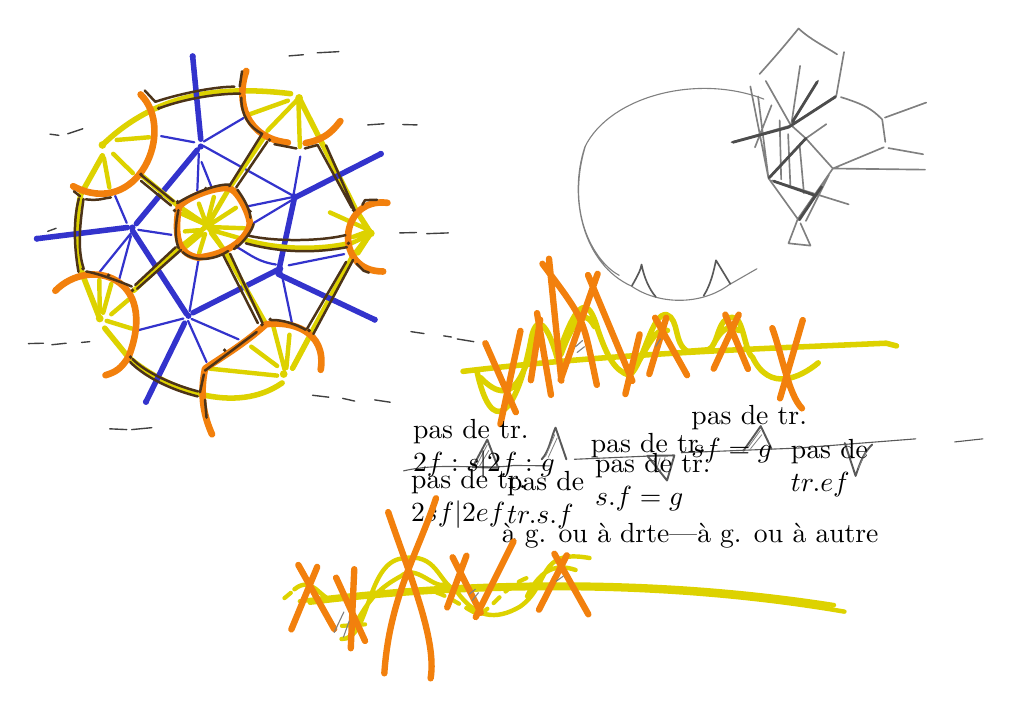
\begin{tikzpicture}[x=.0049cm,y=-.0049cm,line cap=round,line join=round]
\draw[yellow!70!olive,line width=2pt] (550,446)..controls(667,333)and(815,286)..(1038,313) (550,474)--(494,574)..controls(475,665)and(484,723)..(498,781)--(543,896) (556,921)--(617,996)..controls(716,1081)and(895,1148)..(1016,1063) (1043,1025)--(1090,937)--(1198,737)--(1246,675)--(1208,616)--(1060,324);
\draw[yellow!70!olive,line width=1.6pt] (554,480)--(568,556) (578,469)--(629,519) (587,433)--(671,426) (933,366)--(1031,331) (978,409)--(1058,326)--(1062,451) (1140,621)--(1244,668)--(1198,685) (1195,701)--(1244,679)--(1213,727) (991,908)--(1022,1027) (1035,938)--(1027,1024) (936,969)--(1003,1019) (829,1026)--(1003,1044) (626,922)--(561,902) (619,846)--(573,885) (573,806)--(552,881) (542,796)--(543,877);
\draw[blue!60!gray,line width=2pt] (784,216)--(805,431) (796,459)--(638,650) (628,668)--(768,884) (763,908)--(663,1112) (785,881)--(1008,768)--(1048,583)--(1272,469) (1006,781)--(1256,899) (615,660)--(380,689);
\draw[blue!60!gray,line width=.8pt] (702,423)--(788,439) (813,437)--(916,376) (811,448)--(1045,578)--(1063,476) (1049,580)--(927,605) (1046,586)--(941,649) (1010,757)--(1044,920) (1033,758)--(1177,729) (1000,756)..controls(945,748)and(923,721)..(892,708) (800,468)--(796,565) (807,490)--(834,558) (624,675)--(543,775) (624,682)--(594,793) (613,648)--(583,578) (643,666)--(729,679) (772,902)--(820,1009) (781,897)--(903,950) (760,896)--(644,926) (776,877)--(799,744);
\draw[yellow!70!olive,line width=1.8pt] (647,521)--(745,603)--(822,655)--(879,558)--(974,418) (631,824)--(752,711)--(822,655)--(867,721)--(975,912) (919,692)..controls(1022,721)and(1122,716)..(1190,701);
\draw[yellow!70!olive,line width=1.6pt] (757,625)--(820,653)--(800,598) (821,650)--(839,581) (828,653)--(896,609) (833,659)--(919,662) (834,667)--(914,690) (832,675)--(864,717) (816,677)--(801,726) (807,676)--(767,710) (800,667)--(764,670);
\draw[orange!80!brown,line width=2.4pt] (649,315)..controls(742,407)and(644,641)..(474,553) (923,254)..controls(895,334)and(923,428)..(1031,440) (1077,441)..controls(1134,431)and(1154,400)..(1167,384) (428,824)..controls(516,734)and(698,787)..(618,995)..controls(598,1027)and(584,1035)..(558,1043) (1289,596)..controls(1162,580)and(1148,775)..(1278,774) (1116,1029)..controls(1132,928)and(1039,901)..(974,911)..controls(919,961)and(869,990)..(816,1026)..controls(801,1101)and(815,1152)..(834,1196) (748,607)..controls(768,581)and(850,551)..(880,559)..controls(904,566)and(939,640)..(931,658)..controls(912,707)and(854,732)..(798,738)..controls(749,730)and(735,689)..(748,607);
\draw[brown!40!black,line width=.9pt] (660,305)--(687,334)..controls(760,310)and(850,294)..(892,295) (696,351)..controls(772,323)and(859,312)..(907,313) (912,255)--(906,294) (910,323)..controls(910,370)and(931,400)..(964,417)--(879,553) (978,437)--(897,556) (996,444)--(1053,455) (1075,455)--(1108,446)--(1197,609) (1130,447)--(1204,615) (1224,601)--(1231,589)--(1262,588) (1180,680)..controls(1108,697)and(991,696)..(928,681) (1184,711)..controls(1085,730)and(995,721)..(922,701) (1209,754)--(1227,772)--(1241,777) (1200,744)--(1097,936) (1182,749)--(1081,922) (1077,925)..controls(1036,903)and(1005,899)..(987,900) (965,908)--(881,728) (953,908)--(864,733) (950,931)--(816,1031) (813,1041)--(803,1087) (816,1107)--(820,1153) (797,1098)..controls(725,1080)and(660,1047)..(622,1009) (798,1085)..controls(732,1068)and(661,1035)..(628,1001) (640,819)--(754,718) (635,809)--(740,711) (626,813)..controls(573,791)and(528,777)..(508,774) (488,775)..controls(473,691)and(478,625)..(489,585) (501,586)..controls(489,669)and(487,722)..(501,765) (476,566)--(492,579) (507,587)..controls(543,591)and(552,584)..(572,582) (649,523)--(735,592) (650,539)--(728,603) (744,597)..controls(784,571)and(850,546)..(878,549) (747,615)..controls(735,673)and(742,700)..(748,714) (758,724)..controls(795,756)and(852,738)..(876,721) (891,716)..controls(916,701)and(940,664)..(942,651) (934,635)..controls(932,606)and(906,570)..(900,562);
\foreach \x/\y in {550/446,543/896,1020/1040,1246/675,1060/324,822/655}{\fill[yellow!70!olive] (\x,\y) circle (10);}
\foreach \x/\y in {784/216,805/450,628/660,773/889,663/1112,1011/767,1047/579,1272/469,1256/899,380/689}{\fill[blue!60!gray] (\x,\y) circle (8);}
\foreach \x/\y in {696/351,650/522,745/593,737/616,818/559,933/618,898/709,867/978,964/912,985/898,1086/927,1188/701,1201/615,983/433,623/996,628/823,566/784,500/767}{\fill[brown!40!black] (\x,\y) circle (5);}
\draw[black!75,line width=.5pt] (414,418)--(437,421) (460,417)--(499,404) (1034,215)--(1071,212) (1107,207)--(1163,204) (1238,394)--(1280,391) (1329,393)--(1366,394) (1321,674)--(1364,673) (1391,676)--(1447,674) (1350,930)--(1384,935) (1435,941)--(1455,944) (1470,949)--(1513,956) (1095,1095)--(1137,1100) (1173,1103)--(1204,1110) (1256,1107)--(1296,1113) (569,1182)--(613,1184) (626,1184)--(678,1179) (358,961)--(397,960) (419,964)--(456,960) (496,958)--(517,956) (408,670)--(430,662);
\draw[gray,line width=.6pt] (2254,262)..controls(2298,213)and(2325,181)..(2355,144)..controls(2385,172)and(2424,191)..(2455,211) (2473,205)--(2453,318)--(2335,395)--(2270,280) (2359,241)--(2337,388)--(2406,279) (2465,322)..controls(2525,341)and(2545,352)..(2572,380)--(2580,438) (2579,375)--(2686,336) (2576,452)--(2444,507)--(2374,429)--(2336,395)--(2181,439) (2588,454)--(2678,470) (2444,507)--(2683,510) (2277,532)--(2374,429)--(2427,392) (2277,532)--(2353,638)--(2444,507) (2286,538)--(2485,600) (2353,638)--(2329,701)--(2386,707)--(2360,649) (2434,523)--(2374,643) (2250,320)--(2277,532) (2230,294)--(2277,532) (2285,343)--(2242,452) (2306,382)--(2310,535) (2328,418)--(2334,555) (2358,449)--(2369,571);
\draw[black!70,line width=1pt] (2185,439)--(2329,400)--(2451,321) (2340,385)--(2403,283) (2279,531)--(2374,429) (2291,540)--(2398,577) (2357,640)--(2415,554);
\draw[gray,line width=.4pt] (2265,327)..controls(2092,260)and(1865,320)..(1801,451)..controls(1757,583)and(1797,756)..(1922,812)..controls(1991,860)and(2100,863)..(2174,809)--(2247,767) (1802,450)..controls(1748,632)and(1832,754)..(1890,784);
\draw[black!65,line width=.6pt] (1923,811)..controls(1938,785)and(1946,769)..(1948,756)..controls(1954,788)and(1967,819)..(1985,840) (2109,837)..controls(2127,808)and(2134,778)..(2141,745)--(2178,806);
\draw[yellow!70!olive,line width=2pt] (1485,1033)..controls(1868,987)and(2242,975)..(2582,960)--(2609,967) (1521,1032)..controls(1558,1205)and(1623,1157)..(1663,942)..controls(1680,874)and(1710,928)..(1729,998)..controls(1783,835)and(1811,841)..(1835,926)..controls(1858,992)and(1878,1033)..(1917,1043)..controls(1953,1015)and(1974,879)..(2013,886)..controls(2046,897)and(2031,961)..(2067,981)--(2121,977)..controls(2148,967)and(2143,893)..(2183,893)..controls(2213,890)and(2214,980)..(2236,997)..controls(2280,1088)and(2360,1049)..(2406,1011) (1530,1049)..controls(1619,1140)and(1644,1033)..(1678,929) (1739,989)..controls(1786,861)and(1810,888)..(1826,917) (1919,1041)..controls(1957,989)and(1981,914)..(2015,927) (2125,981)..controls(2155,919)and(2173,911)..(2200,927);
\draw[orange!80!brown,line width=2.3pt] (1543,960)--(1622,1139) (1634,928)--(1582,1170) (1677,882)--(1713,1094) (1685,899)--(1661,1056) (1708,741)--(1740,1057) (1691,754)..controls(1805,907)and(1794,889)..(1832,1068) (1834,780)--(1738,1055) (1809,783)--(1924,1058) (1943,937)--(1906,1092) (1983,894)--(2066,1043) (2012,894)--(1968,1040) (2165,886)--(2224,1027) (2200,886)--(2135,1026) (2287,921)..controls(2311,986)and(2329,1094)..(2364,1129) (2366,900)--(2307,1103);
\draw[gray,line width=.4pt] (1777,969)--(1795,953) (1781,984)--(1800,969) (1985,968)--(1997,949);
\draw[black!65,line width=.4pt] (1331,1291)..controls(1431,1268)and(1528,1289)..(1617,1277)--(1709,1278) (1774,1261)--(1981,1252) (2051,1244)--(2352,1232)--(2659,1208) (2760,1216)--(2833,1208);
\draw[black!65,line width=.7pt] (1510,1281)--(1548,1210)--(1576,1283)--cycle (1689,1261)..controls(1709,1241)and(1716,1195)..(1725,1179)--(1753,1261) (1963,1252)--(2014,1316)--(2033,1251)--cycle (2212,1239)--(2257,1175)--(2285,1234) (2475,1219)--(2503,1304)..controls(2515,1268)and(2525,1242)..(2546,1223);
\draw[gray,line width=.3pt] (1519,1279)--(1548,1223) (1527,1280)--(1552,1238) (1699,1253)--(1723,1197) (1706,1256)--(1729,1206) (1982,1258)--(1980,1271) (1996,1257)--(1989,1281) (2009,1256)--(1997,1291) (2223,1232)--(2256,1186) (2231,1233)--(2260,1197) (2510,1284)--(2533,1235);
\node[anchor=west,align=left] at (1330,1234) {\unsure{pas de tr.}\\$\unsure{2f:s|2f:g}$};
\node[anchor=west,align=left] at (1325,1363) {\deleted{\unsure{pas de tr.}}\\\deleted{$\unsure{2sf|2ef}$}};
\node[anchor=west,align=left] at (1574,1367) {\unsure{pas de}\\$\unsure{tr.s.f}$};
\node[anchor=west] at (1560,1459) {\unsure{à g. ou à drte|à g. ou à autre}};
\node[anchor=west] at (1791,1225) {\deleted{\unsure{pas de tr.}}};
\node[anchor=west,align=left] at (1802,1320) {\unsure{pas de tr.}\\$\unsure{s.f=g}$};
\node[anchor=west,align=left] at (2052,1196) {\unsure{pas de tr.}\\$\unsure{sf=g}$};
\node[anchor=west,align=left] at (2310,1284) {\unsure{pas de}\\$\unsure{tr.ef}$};
\draw[yellow!70!olive,line width=1.6pt] (1062,1629)..controls(1463,1578)and(1948,1561)..(2447,1639) (1088,1633)..controls(1479,1586)and(1975,1571)..(2474,1656) (1048,1598)..controls(1094,1560)and(1117,1625)..(1144,1624) (1170,1727)..controls(1244,1730)and(1233,1530)..(1327,1518)..controls(1420,1502)and(1417,1578)..(1470,1605)..controls(1518,1672)and(1569,1680)..(1633,1643)..controls(1713,1586)and(1675,1492)..(1813,1517) (1200,1696)..controls(1237,1637)and(1252,1603)..(1324,1564)..controls(1364,1531)and(1406,1596)..(1438,1586) (1651,1616)..controls(1688,1542)and(1729,1532)..(1777,1548);
\draw[yellow!70!olive,line width=1.5pt,dashed] (1022,1621)--(1052,1596) (1171,1693)--(1231,1689) (1417,1607)..controls(1453,1618)and(1506,1658)..(1528,1664)..controls(1580,1628)and(1598,1585)..(1661,1565);
\draw[orange!80!brown,line width=2.3pt] (1058,1535)--(1151,1701) (1107,1540)--(1040,1702) (1156,1568)--(1231,1732) (1203,1546)--(1194,1751) (1291,1398)..controls(1345,1557)and(1418,1728)..(1401,1829) (1415,1362)..controls(1369,1501)and(1294,1620)..(1281,1816) (1458,1515)--(1531,1659) (1494,1511)--(1444,1645) (1616,1474)--(1518,1670) (1722,1506)--(1810,1663) (1754,1510)--(1682,1651);
\draw[gray,line width=.4pt] (1176,1657)--(1151,1710) (1190,1680)--(1175,1722) (1502,1610)--(1517,1598) (1509,1627)--(1525,1607) (1727,1577)--(1745,1564);
\end{tikzpicture}}
\margin{101}
\scanpage{103}
\begin{verbatim}
*******************************************************************************
*JESNEWS DU 09/08/1982 C68 CADARACHE                                          *
*******************************************************************************
*      DEPUIS LE 1/7/82 LES ALIAS DES COMMANDES LIBRARIAN                     *
*             LIBGET (LG) ET LIBSAVE (LS) SONT SUPPRIMES,                     *
*             POUR EVITER UNE POSSIBILITE DE CONFLIT AVEC                     *
*             LE MEME ALIAS DES COMMANDES STANDARD IBM.                       *
*      ********                                                               *
* ATTENTION                                                                   *
*   MISE EN SERVICE LE VENDREDI 30/7/82 A 8H00 DE LA DEUXIEME PHASE DE GAF    *
*     SUR 168 CADARACHE.                                                      *
*     ELLE PERMET D'UTILISER DANS LA CDE. KEEP TSO ET DANS LA PROCEDURE KEEP  *
*     BATCH UNE POSSIBILITE D'AFFECTATION DE TYPE DE SAUVEGARDE AU NIVEAU DU  *
*     FICHIER.CETTE POSSIBILITE EST VIVEMENT CONSEILLEE.                      *
*     POUR PLUS AMPLES INFORMATIONS VOIR NOTE TECHNIQUE CISI MVS140,LA NOTE   *
*     MVS 143 ETANT SUPPRIMEE.                                                *
*                                                                             *
* EXEMPLES D'UTILISATION:                                                     *
*                                                                             *
*  BATCH:  DSN=NOM.DU.FICHIER.A.SAUVEGARDER,DELAY=TYPE DE SAUVEGARDE          *
*                                                                             *
*  TSO:                                                                       *
*  K DA('NOM DU FICHIER A SAUVEGARDER') DELAY(TYPE DE SAUVEGARDE)             *
*                                                                             *
*  TYPES DE SAUVEGARDE:                                                       *
*                                                                             *
*      W       SAUVEGARDE HEBDO.                                              *
*      D       SAUVEGARDE JOURNALIERE.                                        *
*      NOS     SAUVEGARDE MENSUELLE.                                          *
*      W       PARAMETRE PAR DEFAUT.                                          *
*                                                                             *
*******************************************************************************
\end{verbatim}
\begin{verbatim}
******************************************************************
*                                                                *
*                  - J E S N E W S   F R 1 -      LE 18/08/82    *
*                                                                *
*----------------------------------------------------------------*
*                                                                *
*  DEPUIS LE LUNDI 12 JUILLET 82, LES CLASSES DE TRAVAUX D ET E  *
*  SERONT ETENDUES POUR UNE TAILLE MEMOIRE SUPERIEURE A 1024 K   *
*  SE REPORTER A LA NOTE TECHNIQUE MVS141.                       *
*                                                                *
*----------------------------------------------------------------*
*  A PARTIR DU LUNDI 9 AOUT 1982 , IL SERA POSSIBLE D'IMPRIMER   *
*  SUR XEROX 9700 (DESTINATION SAC) DES FICHIERS UTILISANT LE    *
*  COUPLE DE JEUX DE CARACTERES : (GS15,GT15)                    *
*                                                                *
*----------------------------------------------------------------*
*                                                                *
*-LE 16/08/82 :                                                  *
*----------------------------------------------------------------*
*  -LE 370/168 SERA ARRETE DU VENDREDI 20 AOUT A 19H JUSQU'AU    *
*   LUNDI 23 AOUT A 8H.( MISE A NIVEAU TECHNIQUE.).              *
*                                                                *
*----------------------------------------------------------------*
*                                                                *
*-LE 18/08/82 :                                                  *
*-------------                                                   *
\end{verbatim}
\figure{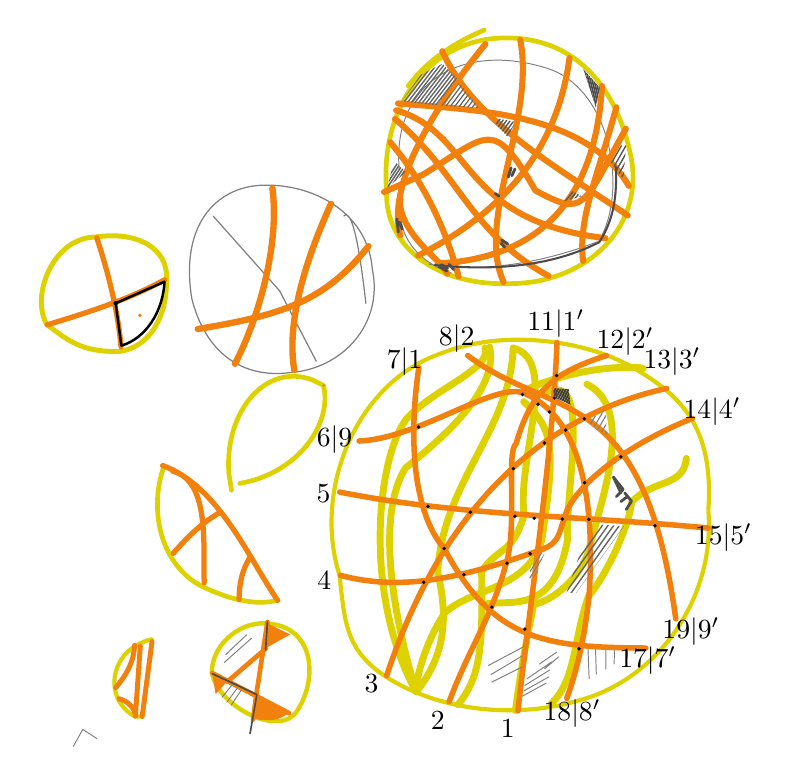
\begin{tikzpicture}[x=.0048cm,y=-.0048cm,line cap=round,line join=round]
\draw[yellow!70!olive,line width=1.7pt] (2020,746)..controls(2000,521)and(2135,339)..(2334,340)..controls(2508,338)and(2622,457)..(2663,642)..controls(2708,832)and(2555,986)..(2351,989)..controls(2135,997)and(2014,877)..(2020,746) (2077,467)..controls(2138,384)and(2226,341)..(2278,319);
\draw[gray,line width=.35pt] (2053,685)..controls(2035,458)and(2219,348)..(2447,421)..controls(2613,477)and(2658,743)..(2582,875) (2063,766)..controls(2038,854)and(2100,932)..(2191,961) (2133,938)..controls(2286,963)and(2451,929)..(2591,873);
\draw[orange!80!brown,line width=2.2pt] (2167,375)..controls(2250,559)and(2457,672)..(2657,809) (2281,356)..controls(2142,527)and(2020,730)..(2056,861) (2373,345)..controls(2414,556)and(2254,819)..(2329,985) (2503,393)..controls(2475,606)and(2358,786)..(2103,915) (2589,467)..controls(2574,723)and(2463,920)..(2155,936) (2627,523)..controls(2573,720)and(2526,817)..(2539,929) (2652,580)..controls(2536,788)and(2545,814)..(2413,743)..controls(2301,549)and(2291,593)..(2116,701)--(2013,747) (2050,513)..controls(2257,531)and(2547,538)..(2660,731) (2045,531)..controls(2254,593)and(2207,822)..(2598,869) (2042,554)..controls(2211,697)and(2240,855)..(2448,969) (2030,616)..controls(2133,738)and(2184,873)..(2210,970) (2057,748)..controls(2038,849)and(2165,924)..(2180,963);
\draw[black!70,line width=.75pt] (2147,940)..controls(2316,957)and(2462,940)..(2579,881) (2581,881)..controls(2622,817)and(2628,757)..(2626,681);
\begin{scope}\clip (2060,507)--(2110,437)--(2167,408)--(2206,447)--(2152,518)--cycle;\foreach \k in {1990,2000,...,2210}{\draw[black!60,line width=.5pt] (\k,530)--++(100,-130);}\end{scope}
\begin{scope}\clip (2164,519)--(2212,459)--(2264,525)--cycle;\foreach \k in {2140,2152,...,2260}{\draw[black!60,line width=.45pt] (\k,537)--++(60,-80);}\end{scope}
\begin{scope}\clip (2292,548)--(2360,562)--(2340,602)--cycle;\foreach \k in {2280,2290,...,2360}{\draw[black!65,line width=.5pt] (\k,608)--++(50,-68);}\end{scope}
\begin{scope}\clip (2540,423)--(2583,471)--(2573,524)--cycle;\foreach \k in {2535,2540,...,2590}{\draw[black!70,line width=.6pt] (\k,415)--++(28,124);}\end{scope}
\begin{scope}\clip (2604,656)--(2654,598)--(2646,715)--cycle;\foreach \k in {2580,2592,...,2670}{\draw[black!65,line width=.5pt] (\k,730)--++(60,-105);}\end{scope}
\begin{scope}\clip (2022,735)--(2039,664)--(2071,695)--cycle;\foreach \k in {2000,2008,...,2075}{\draw[black!60,line width=.55pt] (\k,744)--++(60,-90);}\end{scope}
\begin{scope}\clip (2486,772)--(2509,744)--(2536,758)--cycle;\foreach \k in {2470,2480,...,2540}{\draw[black!65,line width=.5pt] (\k,785)--++(42,-50);}\end{scope}
\draw[black!70,line width=1pt] (2349,683)--(2341,708) (2359,686)--(2351,704) (2307,751)--(2317,758) (2324,874)--(2340,884) (2323,883)--(2332,893) (2047,818)--(2051,853) (2054,827)--(2061,845) (2157,943)--(2179,956) (2164,939)--(2181,948) (2185,938)--(2197,952);
\draw[yellow!70!olive,line width=1.8pt] (1122,1097)..controls(1078,1021)and(1139,866)..(1252,866)..controls(1353,850)and(1446,891)..(1438,982)..controls(1440,1095)and(1374,1178)..(1286,1168)..controls(1207,1165)and(1169,1133)..(1122,1097);
\draw[orange!80!brown,line width=1.9pt] (1254,868)..controls(1291,980)and(1312,1080)..(1318,1156) (1123,1098)..controls(1245,1061)and(1344,1028)..(1433,979);
\draw[black,line width=.9pt] (1433,984)--(1304,1041)--(1319,1153)..controls(1383,1134)and(1429,1064)..(1433,984);
\fill[black] (1304,1041) circle (6);\fill[orange!80!brown] (1368,1073) circle (5);
\draw[gray,line width=.45pt] (1505,1028)..controls(1472,825)and(1578,726)..(1705,729)..controls(1832,729)and(1970,804)..(1982,950)..controls(2013,1098)and(1900,1215)..(1766,1224)..controls(1640,1241)and(1541,1173)..(1505,1028) (1562,811)--(1737,1008)--(1834,1194) (1907,810)..controls(1933,785)and(1954,943)..(1965,1041);
\draw[orange!80!brown,line width=2.3pt] (1718,737)..controls(1738,883)and(1682,1081)..(1619,1201) (1873,778)..controls(1819,897)and(1752,1077)..(1776,1218) (1521,1109)..controls(1745,1072)and(1857,1036)..(1972,890);
\draw[yellow!70!olive,line width=1.7pt] (1603,1490)..controls(1591,1328)and(1700,1196)..(1825,1244)--(1853,1258)..controls(1877,1358)and(1788,1490)..(1632,1517) (1603,1490)--(1610,1535);
\fill[orange!80!brown] (1854,1258) circle (4);
\draw[yellow!70!olive,line width=1.7pt] (1432,1470)..controls(1387,1596)and(1428,1747)..(1547,1796)..controls(1609,1824)and(1674,1840)..(1732,1826);
\draw[orange!80!brown,line width=1.9pt] (1428,1470)..controls(1576,1522)and(1660,1723)..(1732,1826) (1456,1702)..controls(1499,1652)and(1538,1617)..(1581,1593) (1455,1485)..controls(1555,1509)and(1534,1692)..(1538,1780) (1658,1714)..controls(1637,1748)and(1630,1785)..(1630,1824);
\draw[yellow!70!olive,line width=1.5pt] (1399,1929)..controls(1287,1955)and(1268,2086)..(1355,2133)--(1373,2133);
\draw[orange!80!brown,line width=1.8pt] (1400,1935)--(1374,2133) (1369,1947)--(1356,2132) (1354,1945)..controls(1351,1994)and(1330,2025)..(1304,2057) (1313,2086)..controls(1340,2094)and(1355,2113)..(1356,2132);
\draw[yellow!70!olive,line width=1.6pt] (1558,2016)..controls(1559,1937)and(1641,1877)..(1708,1888)..controls(1822,1895)and(1843,2024)..(1784,2117)..controls(1741,2190)and(1575,2110)..(1558,2016);
\draw[orange!80!brown,line width=1.7pt] (1705,1883)--(1675,2079)--(1667,2141) (1559,2018)--(1762,2124) (1599,2041)--(1701,1953);
\fill[orange!80!brown] (1705,1887)--(1765,1916)--(1698,1954)--cycle (1560,2024)--(1598,2041)--(1568,2074)--cycle (1674,2082)--(1762,2123)..controls(1732,2147)and(1706,2145)..(1668,2139)--cycle;
\draw[black!70,line width=.6pt] (1705,1883)--(1700,1957) (1560,2020)--(1677,2075)--(1659,2178);
\draw[gray,line width=.35pt] (1595,1969)--(1650,1917) (1591,1990)--(1663,1926) (1585,2082)--(1613,2048) (1598,2095)--(1625,2058) (1609,2103)--(1636,2063) (1192,2212)--(1217,2167)--(1254,2191);
\draw[yellow!70!olive,line width=1.5pt] (1895,1758)..controls(1826,1540)and(1934,1259)..(2154,1177)..controls(2345,1099)and(2579,1147)..(2694,1225)..controls(2811,1297)and(2884,1384)..(2870,1588)..controls(2889,1826)and(2731,2038)..(2526,2091)..controls(2336,2146)and(2134,2107)..(2011,2023)..controls(1905,1951)and(1909,1866)..(1895,1758);
\draw[yellow!70!olive,line width=2.5pt] (2292,1157)..controls(2316,1268)and(2174,1392)..(2070,1476)..controls(1987,1609)and(2043,1888)..(2098,2068)..controls(2167,1981)and(2187,1888)..(2155,1753)..controls(2166,1514)and(2349,1374)..(2354,1159) (2354,1159)..controls(2478,1192)and(2364,1452)..(2383,1601)..controls(2352,1707)and(2312,1685)..(2271,1750)..controls(2273,1928)and(2274,2023)..(2208,2102) (2389,1269)..controls(2542,1202)and(2680,1208)..(2698,1213) (2382,1301)..controls(2467,1377)and(2464,1436)..(2430,1666)..controls(2392,1799)and(2244,1793)..(2175,1858)..controls(2143,1901)and(2099,2003)..(2098,2068) (2440,1278)..controls(2562,1216)and(2493,1520)..(2498,1665)..controls(2463,1863)and(2350,1825)..(2285,1835) (2549,1255)..controls(2680,1320)and(2585,1566)..(2555,1690)..controls(2534,1768)and(2456,1829)..(2409,1836)..controls(2378,1982)and(2368,2064)..(2360,2117) (2280,1159)..controls(2298,1215)and(2145,1266)..(2072,1347)..controls(1996,1448)and(1955,1805)..(2098,2068) (2455,2099)..controls(2521,2035)and(2513,1930)..(2553,1816)..controls(2606,1752)and(2663,1621)..(2667,1567)..controls(2724,1504)and(2804,1529)..(2812,1451);
\draw[orange!80!brown,line width=2pt] (2105,1211)..controls(2074,1421)and(2097,1603)..(2172,1689)..controls(2300,1928)and(2429,1951)..(2705,1952) (2234,1179)..controls(2461,1351)and(2698,1247)..(2784,1875) (2470,1145)..controls(2460,1435)and(2393,1877)..(2367,2118) (2601,1179)..controls(2469,1222)and(2404,1265)..(2362,1412)..controls(2335,1432)and(2366,1628)..(2336,1728)..controls(2294,1880)and(2241,1945)..(2185,2094) (2760,1266)..controls(2481,1326)and(2183,1530)..(2020,2025) (2828,1345)..controls(2652,1416)and(2528,1516)..(2495,1592)..controls(2469,1666)and(2480,1678)..(2397,1703)..controls(2204,1771)and(2052,1801)..(1898,1760) (2870,1635)..controls(2515,1601)and(2222,1604)..(1896,1540) (1947,1405)..controls(2112,1398)and(2318,1238)..(2390,1282)..controls(2574,1365)and(2563,1687)..(2555,1811)..controls(2545,1910)and(2527,1999)..(2496,2085);
\foreach \x/\y in {2104/1368,2129/1578,2172/1689,2224/1758,2298/1844,2385/1902,2528/1954,2379/1282,2420/1308,2469/1232,2463/1291,2450/1328,2493/1376,2542/1346,2437/1410,2355/1478,2359/1604,2410/1609,2484/1611,2554/1612,2639/1447,2543/1515,2729/1629,2338/1728,2399/1703,2118/1778,2241/1593}{\fill[black] (\x,\y) circle (5);}
\begin{scope}\clip (2459,1265)--(2501,1268)--(2506,1309)--(2463,1290)--cycle;\foreach \k in {2440,2447,...,2510}{\draw[black!75,line width=.7pt] (\k,1316)--++(35,-65);}\end{scope}
\begin{scope}\clip (2546,1352)--(2598,1324)--(2603,1391)--cycle;\foreach \k in {2535,2549,...,2610}{\draw[gray,line width=.4pt] (\k,1400)--++(50,-85);}\end{scope}
\begin{scope}\clip (2557,1624)--(2647,1630)--(2521,1806)--(2495,1807)--cycle;\foreach \k in {2450,2465,...,2670}{\draw[black!60,line width=.5pt] (\k,1824)--++(150,-210);}\end{scope}
\begin{scope}\clip (2402,1710)--(2440,1695)--(2413,1761)--(2397,1768)--cycle;\foreach \k in {2380,2390,...,2450}{\draw[gray,line width=.4pt] (\k,1780)--++(50,-80);}\end{scope}
\draw[black!70,line width=1pt] (2639,1542)--(2619,1500)--(2645,1533)--(2627,1552) (2649,1542)--(2667,1564)--(2653,1586) (2653,1554)--(2639,1565);
\draw[gray,line width=.35pt] (2289,1998)--(2383,1948) (2296,2022)--(2378,1973) (2298,2042)--(2376,2003) (2379,2079)--(2441,2045) (2383,2065)--(2449,2028) (2385,2051)--(2451,2010) (2391,2033)--(2457,1988) (2469,1963)--(2424,1994) (2475,1975)--(2437,2007) (2552,1955)--(2555,2033) (2572,1956)--(2574,2021) (2599,1958)--(2599,2008) (2622,1959)--(2621,1994) (2657,1960)--(2655,1979);
\node at (2067,1194) {$\unsure{7|1}$};\node at (2205,1134) {$\unsure{8|2}$};
\node at (2467,1094) {$\unsure{11|1'}$};\node at (2650,1141) {$\unsure{12|2'}$};\node at (2774,1195) {$\unsure{13|3'}$};\node at (2880,1327) {$\unsure{14|4'}$};
\node at (2910,1660) {$\unsure{15|5'}$};\node at (2824,1908) {$\unsure{19|9'}$};\node at (2710,1985) {$\unsure{17|7'}$};\node at (2510,2124) {$\unsure{18|8'}$};
\node at (2340,2165) {$1$};\node at (2155,2145) {$2$};\node at (1980,2045) {$3$};\node at (1855,1775) {$4$};\node at (1853,1545) {$5$};\node at (1882,1400) {$\unsure{6|9}$};
\end{tikzpicture}}
% crop-candidate: scan 103
\margin{102}
\scanpage{104}
\figure{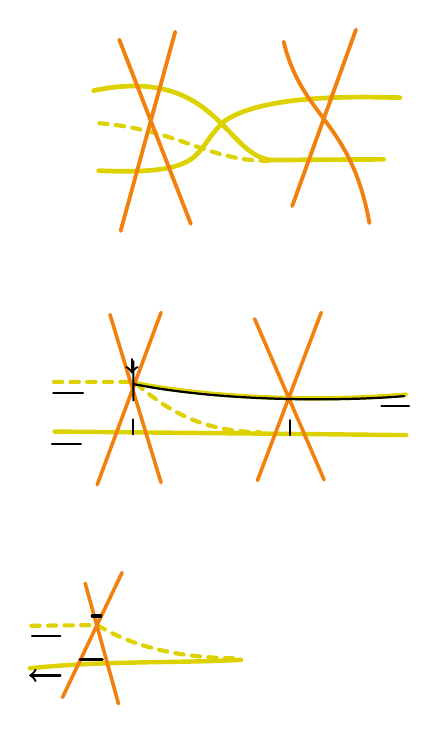
\begin{tikzpicture}[x=.009cm,y=-.009cm,line cap=round,line join=round]
\draw[yellow!70!olive,line width=1.7pt] (329,229)..controls(502,193)and(514,320)..(579,327)--(738,326) (336,342)..controls(497,349)and(466,313)..(515,271)..controls(569,236)and(688,237)..(761,239);
\draw[yellow!70!olive,line width=1.5pt,dashed] (337,275)..controls(451,285)and(492,329)..(576,328);
\draw[orange!80!brown,line width=1.4pt] (365,157)--(466,417) (444,146)--(367,427) (597,160)..controls(623,268)and(692,271)..(718,416) (699,143)--(609,392);
\draw[yellow!70!olive,line width=1.6pt] (274,710)--(770,715) (384,641)..controls(489,662)and(636,669)..(769,658);
\draw[yellow!70!olive,line width=1.5pt,dashed] (273,640)--(386,640)..controls(431,679)and(480,710)..(563,711);
\draw[orange!80!brown,line width=1.3pt] (352,545)--(424,782) (424,542)--(334,785) (556,551)--(654,778) (650,542)--(560,779);
\draw[black,line width=.8pt] (385,611)--(385,666) (385,643)..controls(515,669)and(686,667)..(767,660);
\draw[black,->,line width=.8pt] (272,656)--(314,656) (311,728)--(270,728) (385,714)--(385,693) (606,715)--(606,694) (774,674)--(735,674) (383,608)--(383,628);
\draw[yellow!70!olive,line width=1.6pt] (239,1044)..controls(342,1033)and(445,1037)..(537,1032);
\draw[yellow!70!olive,line width=1.5pt,dashed] (241,984)--(334,983)..controls(392,1018)and(462,1030)..(536,1030);
\draw[orange!80!brown,line width=1.3pt] (317,924)--(364,1094) (369,909)--(285,1085);
\draw[black,line width=1.2pt] (327,970)--(339,970) (310,1032)--(341,1032);
\draw[black,->,line width=.8pt] (242,998)--(282,998) (282,1054)--(238,1054);
\end{tikzpicture}}

Opération de rotation autour d'une face
par une flèche de transition

$(\unsure{\overleftarrow D|D},\omega,a)$, $D$ position relative\inserted{orientée}, $a$ arc de transition sur $\widetilde D$, on
trouve $(D',\omega',a')$ où
\deleted{on balaye sur l'arc de transition,}

a) $D'$ \unsure{déduite|déduit} de $D$ en \unsure{transit$^t$ suiv$^t$} $a$

b) $\omega'$ est l'orientat. \uline{opposée} à celle déduite de $\omega$ par transport

c) $a'$ est l'arc de transition sur $\widetilde D'$, qui \uline{suit} l'arc de
transition transporté de $a$, dans la direction $\omega'$.

\uline{NB} Le balayage du \unsure{lieu} de spécialisation

Le balayage de l'arc de spécialisation

l'antibalay. par des
\figure{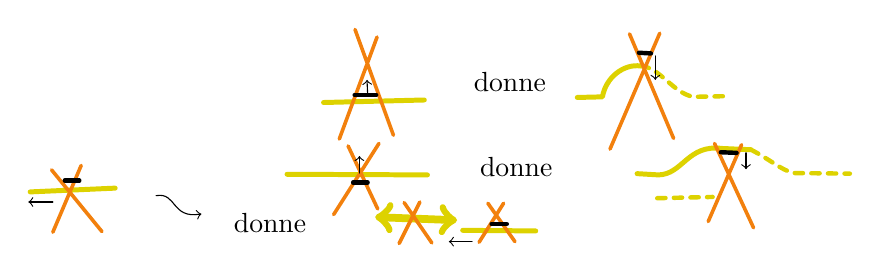
\begin{tikzpicture}[x=.008cm,y=-.008cm,line cap=round,line join=round]
\draw[yellow!70!olive,line width=1.8pt] (1989,928)--(2149,924);
\draw[orange!80!brown,line width=1.3pt] (2039,812)--(2100,980) (2074,824)--(2014,986);
\draw[black,line width=1.4pt] (2038,916)--(2073,916);\draw[black,->] (2059,914)--(2058,892);
\node at (2285,895) {donne};
\draw[yellow!70!olive,line width=1.8pt] (2392,920)--(2432,919)..controls(2437,889)and(2465,866)..(2493,870);
\draw[yellow!70!olive,line width=1.6pt,dashed] (2493,870)..controls(2523,872)and(2543,912)..(2576,919)--(2624,918);
\draw[orange!80!brown,line width=1.3pt] (2475,819)--(2545,985) (2523,818)--(2444,1002);
\draw[black,line width=1.6pt] (2490,849)--(2509,850);\draw[black,->] (2516,854)--(2516,892);
\draw[yellow!70!olive,line width=1.8pt] (1931,1042)--(2154,1043);
\draw[orange!80!brown,line width=1.3pt] (2028,997)--(2075,1097) (2077,993)--(2005,1106);
\draw[black,line width=1.6pt] (2036,1055)--(2059,1055);\draw[black,->] (2046,1040)--(2046,1013);
\node at (2295,1030) {donne};
\draw[yellow!70!olive,line width=1.8pt] (2487,1041)--(2521,1043)..controls(2560,1042)and(2567,994)..(2622,1001)--(2668,1003);
\draw[yellow!70!olive,line width=1.6pt,dashed] (2668,1003)..controls(2699,1019)and(2714,1034)..(2735,1040)--(2825,1041) (2519,1080)--(2607,1078);
\draw[orange!80!brown,line width=1.3pt] (2610,993)--(2672,1127) (2653,995)--(2600,1117);
\draw[black,line width=1.6pt] (2620,1007)--(2645,1008);\draw[black,->] (2660,1008)--(2660,1034);
\draw[yellow!70!olive,line width=1.8pt] (1523,1070)--(1658,1064);
\draw[orange!80!brown,line width=1.3pt] (1557,1035)--(1637,1133) (1604,1028)--(1559,1134);
\draw[black,line width=1.6pt] (1578,1052)--(1601,1052);\draw[black,->] (1559,1086)--(1520,1086);
\draw[black,->] (1723,1076)..controls(1756,1070)and(1747,1113)..(1795,1105);
\node at (1904,1120) {donne};
\draw[yellow!70!olive,line width=2.8pt,<->] (2071,1110)--(2201,1115);
\draw[orange!80!brown,line width=1.3pt] (2117,1087)--(2161,1151) (2142,1086)--(2109,1152);
\draw[yellow!70!olive,line width=1.8pt] (2210,1131)--(2326,1132);
\draw[orange!80!brown,line width=1.3pt] (2250,1088)--(2293,1149) (2275,1088)--(2236,1150);
\draw[black,line width=1.6pt] (2256,1121)--(2280,1121);\draw[black,->] (2225,1149)--(2188,1149);
\end{tikzpicture}}

Pour $\rho(D,\omega,-)=(D',\omega',a')$, \deleted{\unsure{les}}\inserted{\unsure{quatre}} cas à considérer se groupent par deux paires,
correspondant resp. aux cas où $a$ est un arc de spécialisation, un arc de généralisation
\figure{\begin{tikzpicture}[x=.009cm,y=-.009cm,line cap=round,line join=round]
\draw[yellow!70!olive,line width=1.8pt] (650,1458)--(1040,1448);
\draw[orange!80!brown,line width=1.4pt] (698,1331)--(786,1518) (772,1323)--(689,1509);
\draw[orange!80!brown,line width=1.4pt] (895,1288)--(983,1518) (969,1280)--(886,1509);
\draw[black,line width=2pt] (714,1448)--(761,1448);
\node at (778,1425) {$a$};\node at (985,1423) {$a_0^{\prime}$};\node at (1054,1461) {$D$};\node at (558,1493) {1)};\node at (1153,1441) {donne};
\draw[black,->] (654,1481)--(609,1481);\node at (633,1502) {$\omega$};
\draw[black,dotted,line width=1.5pt] (905,1442)--(964,1442);
\draw[yellow!70!olive,line width=1.8pt] (1251,1453)--(1283,1453)..controls(1297,1453)and(1297,1398)..(1357,1398)..controls(1410,1398)and(1404,1453)..(1432,1453)--(1673,1447);
\draw[orange!80!brown,line width=1.4pt] (1314,1319)--(1399,1519) (1393,1309)--(1303,1527);
\draw[orange!80!brown,line width=1.4pt] (1521,1307)--(1606,1519) (1600,1297)--(1510,1527);
\node at (1384,1377) {$b$};\node at (1590,1424) {$a^{\prime}$};\node at (1700,1455) {$D^{\prime}$};
\draw[black,line width=2pt] (1537,1437)--(1580,1437);
\draw[black,dotted,line width=1pt] (1339,1385)--(1373,1385);
\draw[black,->] (1235,1475)--(1275,1475);
\node at (1250,1499) {$\omega^{\prime}$};
\draw[yellow!70!olive,line width=1.8pt] (650,1660)--(1040,1650);
\draw[orange!80!brown,line width=1.4pt] (698,1528)--(786,1720) (772,1520)--(689,1711);
\draw[orange!80!brown,line width=1.4pt] (895,1583)--(983,1720) (969,1575)--(886,1711);
\draw[black,line width=2pt] (714,1650)--(761,1650);
\node at (778,1627) {$a$};\node at (985,1625) {$a_0^{\prime}$};\node at (1054,1663) {$D$};\node at (558,1695) {2)};\node at (1153,1643) {donne};
\draw[black,->] (654,1683)--(609,1683);\node at (633,1704) {$\omega$};
\draw[black,line width=1.8pt] (919,1625)--(942,1625);
\draw[black,line width=2.2pt] (897,1735)--(965,1567);\node at (943,1683) {$\unsure{b}$};
\draw[yellow!70!olive,line width=1.8pt] (1251,1655)--(1283,1655)..controls(1297,1655)and(1297,1600)..(1357,1600)..controls(1410,1600)and(1404,1655)..(1432,1655)--(1673,1649);
\draw[orange!80!brown,line width=1.4pt] (1314,1521)--(1399,1721) (1393,1511)--(1303,1729);
\draw[orange!80!brown,line width=1.4pt] (1521,1583)--(1606,1721) (1600,1573)--(1510,1729);
\node at (1384,1579) {$b$};\node at (1590,1626) {$a^{\prime}$};\node at (1700,1657) {$D^{\prime}$};
\draw[black,line width=2pt] (1553,1634)--(1574,1634);
\draw[black,dotted,line width=1pt] (1339,1587)--(1373,1587);
\draw[black,->] (1235,1677)--(1275,1677);
\node at (1250,1701) {$\omega^{\prime}$};
\draw[yellow!70!olive,line width=1.8pt] (650,1880)--(1040,1870);
\draw[orange!80!brown,line width=1.4pt] (698,1803)--(786,1940) (772,1795)--(689,1931);
\draw[orange!80!brown,line width=1.4pt] (895,1728)--(983,1940) (969,1720)--(886,1931);
\draw[black,line width=2pt] (718,1851)--(742,1851);
\node at (778,1847) {$a$};\node at (985,1845) {$a_0^{\prime}$};\node at (1054,1883) {$D$};\node at (558,1915) {4)};\node at (1153,1863) {donne};
\draw[black,->] (654,1903)--(609,1903);\node at (633,1924) {$\omega$};
\draw[black,dotted,line width=1.5pt] (905,1864)--(964,1864);
\draw[yellow!70!olive,line width=1.8pt] (1251,1875)--(1283,1875)..controls(1297,1875)and(1297,1930)..(1357,1930)..controls(1410,1930)and(1404,1875)..(1432,1875)--(1673,1869);
\draw[orange!80!brown,line width=1.4pt] (1314,1823)--(1399,1941) (1393,1813)--(1303,1949);
\draw[orange!80!brown,line width=1.4pt] (1521,1729)--(1606,1941) (1600,1719)--(1510,1949);
\node at (1384,1909) {$b$};\node at (1590,1846) {$a^{\prime}$};\node at (1700,1877) {$D^{\prime}$};
\draw[black,line width=2pt] (1537,1859)--(1580,1859);
\draw[black,dotted,line width=1pt] (1339,1917)--(1373,1917);
\draw[black,->] (1235,1897)--(1275,1897);
\node at (1250,1921) {$\omega^{\prime}$};
\node at (1361,1954) {$\unsure{*}$};
\draw[yellow!70!olive,line width=1.8pt] (650,2081)--(1040,2071);
\draw[orange!80!brown,line width=1.4pt] (698,2004)--(786,2141) (772,1996)--(689,2132);
\draw[orange!80!brown,line width=1.4pt] (895,2004)--(983,2141) (969,1996)--(886,2132);
\draw[black,line width=2pt] (718,2052)--(742,2052);
\node at (778,2048) {$a$};\node at (985,2046) {$a_0^{\prime}$};\node at (1054,2084) {$D$};\node at (558,2116) {3)};\node at (1153,2064) {donne};
\draw[black,->] (654,2104)--(609,2104);\node at (633,2125) {$\omega$};
\draw[black,line width=1.8pt] (919,2046)--(942,2046);
\draw[yellow!70!olive,line width=1.8pt] (1251,2076)--(1283,2076)..controls(1297,2076)and(1297,2131)..(1357,2131)..controls(1410,2131)and(1404,2076)..(1432,2076)--(1673,2070);
\draw[orange!80!brown,line width=1.4pt] (1314,2024)--(1399,2142) (1393,2014)--(1303,2150);
\draw[orange!80!brown,line width=1.4pt] (1521,2004)--(1606,2142) (1600,1994)--(1510,2150);
\node at (1384,2110) {$b$};\node at (1590,2047) {$a^{\prime}$};\node at (1700,2078) {$D^{\prime}$};
\draw[black,line width=2pt] (1553,2055)--(1574,2055);
\draw[black,dotted,line width=1pt] (1339,2118)--(1373,2118);
\draw[black,->] (1293,2098)--(1255,2098);
\node at (1250,2122) {$\omega^{\prime}$};
\draw[black,line width=.7pt] (535,1445)..controls(536,1520)and(548,1538)..(509,1549)..controls(541,1559)and(516,1655)..(534,1714);
\draw[black,line width=.7pt] (523,1846)..controls(529,1895)and(528,1943)..(501,1955)..controls(536,1974)and(520,2056)..(534,2103);
\node at (449,1551) {$\mathrm{I}$};\node at (442,1958) {$\mathrm{II}$};
\draw[orange!80!brown,line width=.5pt] (1228,2017)--(1261,2028)--(1278,2027)--(1290,2020)--(1301,2059);
\end{tikzpicture}}
Dans tous les cas, pour déterminer
$a'$, on peut soit prendre l'arc $a'_0$\inserted{de transition}
qui suit $a$ sur $\widetilde D$ dans la direction
\uline{opposée} à $\omega$, et prendre son \uline{transporté}
par balayage\inserted{ou antibalayage}; soit transporter d'abord
$a$ en $b$ par la dite opération, et prendre
le successeur de $b$ pour $\omega'$, parmi
les arcs de transition sur $\widetilde D'$.
Cela résulte du fait que dans une
opération de spécialisation, l'isom can. entre
$\mathrm{Pol}(D)$ et $\mathrm{Pol}(D')$ induit une bijection entre
l'ens. des arcs de transition sur le premier,
\margin{103}
\scanpage{105}
\uline{non-adjacents} à \uline{$a$}, sur l'ens des
arcs de transition \deleted{\unsure{sur}} sur $\mathrm{Pol}(D')$
distincts de l'antipodique de $b$.
\figure{\begin{tikzpicture}[x=.0051cm,y=-.0051cm,line cap=round,line join=round]
\draw[yellow!70!olive,line width=1.8pt] (210,524)--(408,524);
\draw[yellow!70!olive,line width=1.8pt] (408,524)--(624,521);
\draw[orange!80!brown,line width=1.4pt] (286,415)--(361,601) (321,413)--(273,593);
\draw[orange!80!brown,line width=1.4pt] (488,415)--(563,601) (523,413)--(475,593);
\draw[black,line width=1.7pt] (295,514)--(333,514);\draw[black,dotted,line width=1.5pt] (499,511)--(543,511);
\draw[orange!80!brown,line width=.9pt] (387,477)--(395,560);
\draw[orange!80!brown,line width=.9pt] (417,474)--(425,560);
\draw[orange!80!brown,line width=.9pt] (447,471)--(455,560);
\draw[black,->,line width=.8pt] (220,547)--(186,547);
\draw[black,|->,line width=1pt] (645,475)--(696,473);
\node at (515,647) {(1)};
\draw[gray,line width=.35pt] (243,513)--(295,387);
\draw[gray,line width=.35pt] (270,513)--(322,387);
\draw[gray,line width=.35pt] (297,513)--(349,387);
\draw[gray,line width=.35pt] (324,513)--(376,387);
\draw[gray,line width=.35pt] (351,513)--(403,387);
\draw[gray,line width=.35pt] (445,513)--(497,387);
\draw[gray,line width=.35pt] (472,513)--(524,387);
\draw[gray,line width=.35pt] (499,513)--(551,387);
\draw[gray,line width=.35pt] (526,513)--(578,387);
\draw[gray,line width=.35pt] (553,513)--(605,387);
\node at (463,648) {$\deleted{\unsure{\mathrm{II}|\mathrm{I}}}$};
\draw[yellow!70!olive,line width=1.8pt] (713,520)..controls(788,532)and(733,440)..(813,437)..controls(877,438)and(872,517)..(910,516);
\draw[yellow!70!olive,line width=1.8pt] (911,520)--(1127,517);
\draw[orange!80!brown,line width=1.4pt] (789,387)--(864,597) (824,385)--(776,589);
\draw[orange!80!brown,line width=1.4pt] (991,411)--(1066,597) (1026,409)--(978,589);
\draw[black,line width=1.7pt] (809,407)--(827,407) (995,507)--(1046,507);
\draw[orange!80!brown,line width=.9pt] (890,473)--(898,556);
\draw[orange!80!brown,line width=.9pt] (920,470)--(928,556);
\draw[orange!80!brown,line width=.9pt] (950,467)--(958,556);
\draw[black,->,line width=.8pt] (1090,538)--(1140,538);
\draw[black,|->,line width=1pt] (1148,471)--(1199,469);
\node at (1018,643) {(2)};
\draw[gray,line width=.35pt] (746,594)--(798,468);
\draw[gray,line width=.35pt] (773,594)--(825,468);
\draw[gray,line width=.35pt] (800,594)--(852,468);
\draw[gray,line width=.35pt] (827,594)--(879,468);
\draw[gray,line width=.35pt] (854,594)--(906,468);
\draw[gray,line width=.35pt] (948,509)--(1000,383);
\draw[gray,line width=.35pt] (975,509)--(1027,383);
\draw[gray,line width=.35pt] (1002,509)--(1054,383);
\draw[gray,line width=.35pt] (1029,509)--(1081,383);
\draw[gray,line width=.35pt] (1056,509)--(1108,383);
\node at (966,644) {$\deleted{\unsure{\mathrm{II}|\mathrm{I}}}$};
\draw[yellow!70!olive,line width=1.8pt] (1228,496)..controls(1303,508)and(1248,416)..(1328,413)..controls(1392,414)and(1387,493)..(1425,492);
\draw[yellow!70!olive,line width=1.8pt] (1426,496)..controls(1486,500)and(1448,397)..(1530,403)..controls(1626,397)and(1628,490)..(1644,493)--(1702,490);
\draw[orange!80!brown,line width=1.4pt] (1304,363)--(1379,573) (1339,361)--(1291,565);
\draw[orange!80!brown,line width=1.4pt] (1506,363)--(1581,573) (1541,361)--(1493,565);
\draw[black,line width=1.7pt] (1324,383)--(1342,383) (1527,384)--(1542,384);
\draw[orange!80!brown,line width=.9pt] (1405,449)--(1413,532);
\draw[orange!80!brown,line width=.9pt] (1435,446)--(1443,532);
\draw[orange!80!brown,line width=.9pt] (1465,443)--(1473,532);
\draw[black,->,line width=.8pt] (1238,519)--(1204,519);
\draw[black,|->,line width=1pt] (1663,447)--(1714,445);
\node at (1533,619) {(3)};
\draw[gray,line width=.35pt] (1261,570)--(1313,444);
\draw[gray,line width=.35pt] (1288,570)--(1340,444);
\draw[gray,line width=.35pt] (1315,570)--(1367,444);
\draw[gray,line width=.35pt] (1342,570)--(1394,444);
\draw[gray,line width=.35pt] (1369,570)--(1421,444);
\draw[gray,line width=.35pt] (1463,570)--(1515,444);
\draw[gray,line width=.35pt] (1490,570)--(1542,444);
\draw[gray,line width=.35pt] (1517,570)--(1569,444);
\draw[gray,line width=.35pt] (1544,570)--(1596,444);
\draw[gray,line width=.35pt] (1571,570)--(1623,444);
\node at (1481,620) {$\deleted{\unsure{\mathrm{II}|\mathrm{I}}}$};
\draw[yellow!70!olive,line width=1.8pt] (1812,478)--(2010,478);
\draw[yellow!70!olive,line width=1.8pt] (2010,478)..controls(2070,482)and(2032,379)..(2114,385)..controls(2210,379)and(2212,472)..(2228,475)--(2286,472);
\draw[orange!80!brown,line width=1.4pt] (1888,369)--(1963,555) (1923,367)--(1875,547);
\draw[orange!80!brown,line width=1.4pt] (2090,345)--(2165,555) (2125,343)--(2077,547);
\draw[black,dotted,line width=1.5pt] (1893,468)--(1939,468);\draw[black,line width=1.7pt] (2109,366)--(2129,366);
\draw[orange!80!brown,line width=.9pt] (1989,431)--(1997,514);
\draw[orange!80!brown,line width=.9pt] (2019,428)--(2027,514);
\draw[orange!80!brown,line width=.9pt] (2049,425)--(2057,514);
\draw[black,->,line width=.8pt] (2189,496)--(2239,496);
\draw[black,|->,line width=1pt] (2247,429)--(2298,427);
\node at (2117,601) {(4)};
\draw[gray,line width=.35pt] (1845,467)--(1897,341);
\draw[gray,line width=.35pt] (1872,467)--(1924,341);
\draw[gray,line width=.35pt] (1899,467)--(1951,341);
\draw[gray,line width=.35pt] (1926,467)--(1978,341);
\draw[gray,line width=.35pt] (1953,467)--(2005,341);
\draw[gray,line width=.35pt] (2047,552)--(2099,426);
\draw[gray,line width=.35pt] (2074,552)--(2126,426);
\draw[gray,line width=.35pt] (2101,552)--(2153,426);
\draw[gray,line width=.35pt] (2128,552)--(2180,426);
\draw[gray,line width=.35pt] (2155,552)--(2207,426);
\draw[yellow!70!olive,line width=1.8pt] (2364,476)--(2562,476);
\draw[yellow!70!olive,line width=1.8pt] (2562,476)--(2778,473);
\draw[orange!80!brown,line width=1.4pt] (2440,367)--(2515,553) (2475,365)--(2427,545);
\draw[orange!80!brown,line width=1.4pt] (2642,367)--(2717,553) (2677,365)--(2629,545);
\draw[black,line width=1.7pt] (2449,466)--(2487,466);\draw[black,dotted,line width=1.5pt] (2653,463)--(2697,463);
\draw[orange!80!brown,line width=.9pt] (2541,429)--(2549,512);
\draw[orange!80!brown,line width=.9pt] (2571,426)--(2579,512);
\draw[orange!80!brown,line width=.9pt] (2601,423)--(2609,512);
\draw[black,->,line width=.8pt] (2374,499)--(2340,499);
\node at (2669,599) {(1)};
\draw[gray,line width=.35pt] (2397,465)--(2449,339);
\draw[gray,line width=.35pt] (2424,465)--(2476,339);
\draw[gray,line width=.35pt] (2451,465)--(2503,339);
\draw[gray,line width=.35pt] (2478,465)--(2530,339);
\draw[gray,line width=.35pt] (2505,465)--(2557,339);
\draw[gray,line width=.35pt] (2599,465)--(2651,339);
\draw[gray,line width=.35pt] (2626,465)--(2678,339);
\draw[gray,line width=.35pt] (2653,465)--(2705,339);
\draw[gray,line width=.35pt] (2680,465)--(2732,339);
\draw[gray,line width=.35pt] (2707,465)--(2759,339);
\node at (350,505) {$a$};\node at (569,503) {$b$};\node at (351,387) {$\lambda^{\prime}$};\node at (479,396) {$\mu^{\prime}$};\node at (353,629) {$\lambda$};\node at (485,609) {$\mu$};
\node at (245,448) {\textcircled{1}};\node at (583,417) {\textcircled{$4^{\prime}$}};\node at (799,590) {\textcircled{$1^{\prime}$}};\node at (1064,406) {\textcircled{2}};\node at (1348,516) {$3$};\node at (1567,529) {\textcircled{$2^{\prime}$}};\node at (1925,358) {\textcircled{$3=1$}};\node at (2098,504) {$4$};\node at (2505,306) {\textcircled{$5=1$}};\node at (2753,389) {$4^{\prime}$};
\node at (329,560) {$x$};\node at (397,546) {$\alpha$};\node at (427,546) {$\beta$};\node at (458,546) {$\unsure{\gamma}$};\node at (789,415) {$\unsure{\lambda^{\prime}}$};
\draw[black,->,line width=.5pt] (388,540)--(391,557) (430,544)--(432,560) (462,547)--(465,565) (1407,480)--(1412,495) (1461,481)--(1465,498) (1988,447)--(1988,431) (2018,407)--(2018,394) (2046,402)--(2046,389) (2548,506)--(2548,515) (2570,506)--(2570,515) (2595,505)--(2595,514);
\draw[black,line width=.6pt] (373,547)--(400,489) (374,551)--(402,496) (387,500)--(405,491);
\end{tikzpicture}}
\uline{NB} Pour chaque position $(D,a,\omega)$ dans le cycle, on a indiqué en pointillé l'arc de
transition $b$ qui suit \unsure{$a$} suivant l'orientation $-\omega$.

Il faudrait regarder à part le cas où on part avec un arc de \deleted{transition}\inserted{spécialisation},
exceptionnel, correspondant à un balayage de couloir. Il ne devrait pas y
avoir de différence.

\margin{\diagram{\begin{array}{r}\text{arcs de spécialisation}\\\text{arcs de généralisation}\end{array}\left\}\vphantom{\begin{array}{r}1\\2\end{array}}\right.\ \text{arcs de transition}}}
\margin{\uline{arcs \deleted{\unsure{de combinatoire}}\inserted{d'isomorphie}}}

\margin{$\geq \unsure{\nu|r}-2+(2\unsure{+|,}2)=2\unsure{\nu|r}+2$\\dont}
\figure{\begin{tikzpicture}[x=.006cm,y=-.006cm,line cap=round,line join=round]
\draw[yellow!70!olive,line width=1.8pt] (256,1577)--(840,1536) (400,1410)--(590,1404) (400,1410)..controls(483,1493)and(542,1517)..(647,1542) (397,1559)--(592,1407);
\draw[orange!80!brown,line width=1.4pt] (368,1322)--(468,1646) (423,1306)--(360,1630) (563,1307)--(671,1644) (617,1295)--(553,1652);
\draw[black,dashed,line width=1.8pt] (399,1410)--(591,1405) (400,1410)..controls(488,1504)and(534,1501)..(574,1533) (450,1556)--(590,1407) (385,1565)--(572,1550);
\draw[black,->,line width=.8pt] (410,1422)--(459,1469) (310,1599)--(254,1599) (709,1562)--(775,1562);
\draw[gray,line width=.35pt] (396,1418)--(344,1480) (409,1436)--(371,1506) (443,1470)--(412,1514);
\node at (367,1409) {$\unsure{x^{\prime}|z^{\prime}}$};\node at (625,1394) {$y^{\prime}$};\node at (349,1584) {$x$};\node at (669,1569) {$y$};\node at (472,1532) {$\unsure{o}$};
\draw[yellow!70!olive,line width=1.8pt] (947,1568)--(1410,1553) (1041,1421)..controls(1077,1420)and(1083,1539)..(1100,1551)--(1207,1551);
\draw[orange!80!brown,line width=1.4pt] (1008,1318)--(1103,1641) (1074,1296)--(992,1664) (1217,1298)--(1335,1665) (1278,1273)--(1218,1637);
\draw[black,dashed,line width=1.6pt] (1043,1421)..controls(1075,1423)and(1084,1537)..(1100,1550) (1100,1550)--(1216,1542)..controls(1235,1463)and(1225,1418)..(1251,1405);
\draw[black,line width=1.4pt] (1212,1443)..controls(1223,1418)and(1231,1411)..(1251,1405) (1008,1564)--(1279,1555);
\foreach \x in {1012,1026,1040,1054,1068,1082,1096,1110,1124,1138,1152,1166,1180,1194,1208,1222,1236,1250,1264}{\draw[black,line width=.4pt] (\x,1557)--++(9,-12);}
\node at (1010,1419) {$z$};\node at (1286,1386) {$t$};\node at (988,1584) {$x$};\node at (1328,1584) {$y$};\node at (933,1637) {$(3)$};
\draw[yellow!70!olive,line width=1.8pt] (811,1738)--(1074,1729)--(1078,1912)--(816,1922)--cycle;
\draw[orange!80!brown,line width=1.4pt] (941,1827)--(811,1738) (941,1827)--(893,1734) (941,1827)--(942,1734) (941,1827)--(991,1732) (941,1827)--(1074,1729) (941,1827)--(1075,1792) (941,1827)--(1077,1827) (941,1827)--(1077,1862) (941,1827)--(1078,1912) (941,1827)--(977,1917) (941,1827)--(941,1918) (941,1827)--(905,1919) (941,1827)--(816,1922) (941,1827)--(815,1849) (941,1827)--(814,1812) (941,1827)--(813,1787);
\fill[black] (941,1827) circle (7);
\draw[black,->,line width=1pt] (814,1740)--(860,1773) (896,1736)--(912,1771) (944,1738)--(946,1770) (991,1735)--(978,1773) (1072,1730)--(1027,1764) (1072,1794)--(1034,1804) (1074,1824)--(1040,1825) (1074,1859)--(1035,1846) (1075,1908)--(1040,1876) (975,1914)--(962,1878) (940,1915)--(941,1879) (906,1918)--(918,1881) (818,1916)--(859,1884) (861,1843)--(815,1849) (858,1815)--(813,1813) (857,1801)--(813,1787);
\node at (782,1735) {$y^{\prime}$};\node at (1095,1729) {$x^{\prime}$};\node at (794,1942) {$x$};\node at (1094,1923) {$y$};
\node at (895,1705) {$\unsure{\gamma|\delta}$};\node at (944,1704) {$\beta$};\node at (1005,1705) {$\alpha$};\node at (1095,1792) {$\alpha$};\node at (1108,1828) {$\beta$};\node at (1101,1861) {$\unsure{\gamma|\delta}$};\node at (978,1945) {$\unsure{\gamma|\delta}$};\node at (945,1948) {$\beta$};\node at (901,1945) {$\alpha$};\node at (782,1787) {$\unsure{\gamma|\delta}$};\node at (782,1819) {$\beta$};\node at (782,1854) {$\alpha$};
\node at (838,1754) {$\mu$};\node at (1046,1768) {$\lambda$};\node at (1038,1880) {$\mu^{\prime}$};\node at (858,1881) {$\unsure{\lambda^{\prime}}$};\node at (1184,1842) {$(2)$};\node at (940,2003) {$(1)$};
\draw[yellow!70!olive,line width=1.7pt] (317,1781)--(548,1759)--(549,1944)--(318,1958)--cycle (154,1630)--(242,1620)--(249,1698)--(181,1710) (162,1702)--(154,1630) (595,1596)--(616,1676)--(713,1652) (596,1588)--(695,1567)--(743,1642) (153,2031)--(263,2030)--(270,2147)--(134,2142)--cycle (616,2023)--(754,2001) (768,2024)--(774,2149) (617,2030)--(616,2134)--(753,2153);
\draw[green!25!black,line width=2.5pt] (250,1699)--(306,1776) (551,1756)--(616,1678) (320,1959)--(253,2027) (548,1942)--(617,2020);
\draw[orange!80!brown,line width=1.2pt] (273,1648)--(199,1828) (174,1804)--(307,1774)..controls(344,1756)and(350,1724)..(374,1719) (585,1636)--(657,1780) (520,1744)--(689,1786) (223,1876)--(255,2027) (190,1907)--(320,1957) (656,1836)--(594,2083) (512,1963)..controls(564,1918)and(616,1910)..(691,1888);
\draw[black,line width=.8pt] (320,1957)--(448,1850)--(551,1758) (306,1774)..controls(336,1768)and(348,1735)..(375,1722) (478,1799)--(519,1714) (552,1743)--(548,1758) (248,1701)--(302,1773) (316,1876)..controls(378,1871)and(402,1854)..(448,1850) (449,1850)--(548,1851) (322,1955)..controls(353,1899)and(373,1884)..(448,1850) (448,1850)..controls(481,1816)and(512,1784)..(550,1759);
\fill[black] (318,1876) circle (6);\draw[black] (450,1850) circle (5);\draw[black] (465,1844) circle (4);
\foreach \x in {380,401,421,439,460,480}{\draw[black!65,line width=.45pt] (\x,1778)--(448,1850)--(\x,1951);}
\foreach \y in {1790,1803,1816,1829,1842,1855,1868,1881,1894,1907,1920,1933,1946}{\draw[black!65,line width=.45pt] (319,\y)--(448,1850)--(548,\y);}
\draw[black,->,line width=.9pt] (321,1869)--(400,1857) (545,1854)--(478,1853) (381,1777)--(381,1833)--(420,1844) (377,1948)--(378,1893) (544,1790)--(513,1793)--(496,1813);
\draw[black,line width=.5pt] (331,1812)--(319,1808)--(351,1823) (342,1836)--(367,1832) (331,1909)--(369,1889) (524,1885)--(545,1895) (504,1905)--(543,1911);
\draw[gray,line width=.4pt] (237,1709)--(270,1772)--(272,1903)--(351,2072) (258,2029)..controls(291,2056)and(361,2078)..(435,2116) (260,2042)..controls(349,2120)and(377,2076)..(438,2116) (263,2054)..controls(332,2114)and(379,2094)..(409,2128) (550,1951)..controls(535,2018)and(515,2048)..(476,2083) (553,1935)--(572,1965) (566,1944)--(584,1972) (577,1953)--(593,1981);
\node at (300,1747) {$y^{\prime}$};\node at (563,1735) {$x^{\prime}$};\node at (298,1993) {$\unsure{x}$};\node at (569,1980) {$\unsure{y}$};\node at (376,1742) {$\unsure{\gamma|\theta}$};\node at (433,1739) {$\beta$};\node at (489,1734) {$\alpha$};\node[draw,ellipse] at (448,1696) {$\unsure{3}$};
\node at (572,1800) {$\alpha$};\node at (574,1855) {$\beta$};\node at (575,1900) {$\unsure{\gamma}$};\node at (386,1986) {$\alpha$};\node at (435,1990) {$\beta$};\node at (482,1987) {$\unsure{\gamma}$};\node at (282,1825) {$\unsure{\gamma}$};\node at (282,1886) {$\beta$};\node at (281,1940) {$\alpha$};\node at (678,1875) {$(4)$};\node at (469,2034) {$(1)$};\node at (447,1874) {$\unsure{o}$};
\draw[yellow!70!olive,line width=1.7pt] (1116,2024)--(1308,2015)--(1329,2164)--(1118,2174)--cycle;
\draw[gray,->,line width=.4pt] (1299,2026)--(1261,2069) (1123,2167)--(1174,2134) (1324,2157)--(1271,2135);
\node at (1338,2006) {$x^{\prime}$};\node at (1108,2191) {$x$};\node at (1339,2190) {$y$};\node at (1171,2121) {$\lambda$};\node at (1250,2121) {$\mu$};
\draw[yellow!70!olive,line width=1.7pt] (1660,1506)--(1691,1501)--(1723,1363)--(1810,1331)..controls(1840,1299)and(1873,1282)..(1914,1298) (1961,1304)..controls(2021,1288)and(2007,1356)..(2042,1422)--(2055,1471)--(2098,1466);
\draw[orange!80!brown,line width=1.1pt] (1654,1369)..controls(1660,1494)and(1716,1634)..(1761,1740) (1705,1347)--(1613,1736) (2105,1314)--(1971,1738) (2019,1282)..controls(2042,1396)and(2103,1601)..(2136,1719) (1705,1347)--(1811,1309) (1837,1304)--(1837,1384) (1837,1304)..controls(1885,1243)and(1896,1268)..(1941,1281)..controls(1961,1225)and(1986,1277)..(2019,1282) (1837,1304)--(1847,1774) (1882,1263)--(1925,1756) (1940,1281)--(1946,1776) (1634,1573)--(1713,1655) (1678,1634)--(1765,1650) (1786,1645)--(1870,1685)--(1966,1643);
\draw[orange!80!brown,line width=1.1pt] (1412,1820)--(1493,2073) (1494,1758)--(1387,2078) (1640,1800)--(1722,2092) (1705,1780)--(1628,2101) (1531,1756)--(1530,2056) (1571,1755)--(1583,2058) (1600,1757)--(1613,2069) (1517,1770)--(1540,1755) (1556,1757)--(1585,1758) (1591,1755)--(1615,1760);
\draw[orange!80!brown,line width=1.1pt] (1964,1853)--(2066,2001) (2043,1822)--(1963,2037) (2437,1790)--(2573,1950) (2552,1781)--(2442,1989) (2154,1744)--(2162,2014) (2208,1740)--(2222,2018) (2264,1733)--(2274,2016) (2331,1748)--(2334,1996);
\draw[orange!80!brown,line width=1.3pt] (2144,1792)--(2164,1791) (2196,1796)--(2226,1796) (2256,1791)--(2280,1790) (2322,1789)--(2340,1789) (2155,1987)--(2170,1987) (2214,1992)--(2233,1992) (2267,1991)--(2283,1991) (2326,1984)--(2342,1984);
\draw[yellow!70!olive,line width=1.7pt] (1957,1925)..controls(1989,1922)and(1970,1986)..(2053,1934) (1957,1925)..controls(2174,1927)and(2334,1917)..(2437,1904)..controls(2476,1937)and(2500,1908)..(2570,1887);
\draw[green!20!black,line width=3pt,->] (2004,1923)..controls(2211,1929)and(2398,1902)..(2564,1888);
\draw[green!20!black,line width=2.5pt] (2024,1954)--(2056,1932);
\foreach \x in {2114,2125,2136,2155,2182,2203,2224,2246,2267,2287,2307,2328,2348,2371,2391,2412}{\draw[black,line width=.4pt] (\x,1904)--++(8,-12);}
\draw[gray,line width=.45pt] (2039,1815)..controls(2125,1707)and(2378,1704)..(2443,1777) (2151,1714)--(2454,1752);
\draw[black,->,line width=.4pt] (2227,1651)--(2222,1779) (2233,1648)--(2240,1778);
\node at (2244,1617) {$\unsure{\nu-2|r-2}$};\node at (2011,2078) {$2$};\node at (2501,2039) {$2$};
\draw[black,line width=.5pt] (2156,2034)..controls(2170,2058)and(2240,2028)..(2254,2063)..controls(2256,2045)and(2350,2055)..(2347,2026);
\node at (2260,2093) {$\unsure{\nu|r}$};
\draw[orange!70!brown,line width=.4pt] (2187,2121)..controls(2444,2125)and(2724,2201)..(2881,2210);
\end{tikzpicture}}

\margin{104}
\scanpage{106}
\figure{\begin{tikzpicture}[x=.006cm,y=-.006cm,line cap=round,line join=round]
\draw[black!55,line width=.6pt] (418,407)..controls(418,297)and(485,230)..(589,229)..controls(693,230)and(749,286)..(745,381)..controls(737,486)and(651,575)..(573,575)..controls(489,573)and(419,505)..(418,407);
\draw[black!55,line width=.55pt] (585,237)..controls(547,335)and(521,451)..(561,519)..controls(597,556)and(597,605)..(596,654) (616,232)..controls(632,355)and(631,454)..(570,537)..controls(520,632)and(507,742)..(514,840)..controls(515,876)and(522,900)..(537,919) (418,405)..controls(439,476)and(490,536)..(544,569) (578,236)--(581,246)--(590,237);
\draw[black!55,line width=.55pt] (398,679)..controls(447,594)and(505,568)..(574,575)..controls(689,570)and(724,668)..(700,785)..controls(683,866)and(607,916)..(537,916)..controls(451,920)and(375,849)..(388,732)..controls(389,713)and(394,694)..(398,679) (630,585)..controls(534,653)and(461,647)..(429,873) (674,623)..controls(596,707)and(522,773)..(411,830) (398,678)..controls(456,669)and(540,703)..(693,805) (593,657)..controls(604,747)and(591,846)..(569,910);
\draw[black!55,line width=.55pt] (134,890)..controls(173,815)and(288,791)..(377,817)..controls(471,842)and(479,971)..(450,1043)..controls(408,1145)and(285,1180)..(216,1152)..controls(115,1117)and(92,1002)..(119,930)..controls(123,916)and(128,899)..(134,890) (137,891)..controls(223,961)and(360,1018)..(453,1035) (143,1068)..controls(206,971)and(267,902)..(411,832) (185,1117)..controls(276,1056)and(365,974)..(426,881) (142,1114)..controls(229,1120)and(289,1069)..(335,1028) (135,864)..controls(242,844)and(327,908)..(449,982) (329,804)--(349,969) (414,817)--(407,850) (420,819)--(416,858) (426,823)--(421,867) (451,961)--(460,1007);
\draw[black!55,line width=.55pt] (495,1083)..controls(504,963)and(511,910)..(570,906)..controls(700,892)and(730,998)..(724,1098)..controls(724,1228)and(663,1298)..(575,1266)..controls(487,1260)and(478,1180)..(495,1083) (537,921)..controls(564,1033)and(533,1107)..(568,1269) (568,911)..controls(577,998)and(619,1008)..(623,1269) (540,922)..controls(492,1013)and(501,1180)..(512,1219) (578,910)..controls(659,910)and(707,933)..(736,973);
\draw[black!45,line width=.5pt] (318,1575)..controls(319,1506)and(410,1424)..(486,1426)..controls(582,1431)and(600,1493)..(606,1587)..controls(616,1688)and(530,1754)..(449,1734)..controls(365,1737)and(309,1677)..(318,1575) (484,1432)..controls(426,1526)and(411,1656)..(438,1729) (490,1436)..controls(562,1512)and(554,1625)..(481,1730) (388,1713)..controls(447,1733)and(517,1729)..(558,1695) (491,1438)--(520,1513) (500,1446)--(530,1518);
\end{tikzpicture}}
\margin{105}
\scanpage{107}
\figure{\begin{tikzpicture}[x=.005cm,y=-.005cm,line cap=round,line join=round]
\draw[yellow!70!olive,line width=1.8pt] (226,524)--(859,512);
\draw[yellow!70!olive,line width=1.8pt,dashed] (236,489)--(849,467);
\draw[orange!80!brown,line width=1.4pt] (351,249)--(440,600) (416,237)--(309,598) (658,246)--(757,616) (731,238)--(623,607) (489,309)--(489,629) (532,298)--(537,620) (570,296)--(570,629);
\draw[black,line width=1.8pt] (339,485)--(409,486);
\draw[black,->,line width=.6pt] (428,566)--(439,605) (484,569)--(484,603) (533,570)--(533,604) (569,566)--(569,603) (633,574)--(619,611);
\fill[black] (652,473) circle (4);
\node at (326,471) {$x_0$};\node at (426,482) {$\unsure{x}$};\node at (440,627) {$\lambda$};\node at (498,641) {$\alpha$};\node at (535,641) {$\beta$};\node at (572,638) {$\gamma$};\node at (620,633) {$\mu$};
\draw[gray,line width=.45pt] (232,479)--(393,308) (296,454)--(441,301) (346,482)--(510,313) (363,478)--(533,316) (420,467)--(585,303) (448,467)--(634,307) (499,463)--(664,299) (518,465)--(688,297) (562,463)--(724,310) (611,463)--(791,285) (665,466)--(829,312) (711,458)--(875,333) (776,454)--(884,377);
\draw[yellow!70!olive,line width=1.8pt] (977,436)--(1104,436)..controls(1119,393)and(1113,357)..(1199,354)..controls(1281,344)and(1276,437)..(1294,453)--(1737,463) (976,520)--(1086,520)..controls(1116,434)and(1108,354)..(1199,354) (1232,356)..controls(1280,362)and(1295,529)..(1325,528)--(1675,530);
\draw[yellow!70!olive,line width=1.8pt,dashed] (991,472)--(1117,472) (1239,482)--(1733,491);
\draw[orange!80!brown,line width=1.4pt] (1179,263)--(1261,613) (1228,254)--(1133,620) (1519,272)--(1634,658) (1586,254)--(1476,637) (1328,263)--(1332,642) (1395,256)--(1383,664) (1431,266)--(1425,641);
\draw[black,line width=1.8pt] (1154,475)--(1234,476) (1514,484)--(1599,487);
\draw[gray,line width=.5pt] (1538,440)--(1574,438) (1480,517)..controls(1501,521)and(1503,487)..(1514,481);
\draw[black,->,line width=.5pt] (1325,365)--(1328,342) (1382,360)--(1391,338) (1428,357)--(1431,338);
\node at (1230,390) {$-\lambda$};\node at (1308,326) {$-\alpha$};\node at (1386,318) {$-\beta$};\node at (1452,315) {$-\gamma$};\node at (1514,391) {$-\mu$};
\node at (1178,453) {$\unsure{x'_0=x_0}$};\node at (1255,451) {$\unsure{x'=x}$};\node at (1507,485) {$y^{\prime}$};\node at (1625,476) {$z^{\prime}$};\node at (1558,532) {$\unsure{e}$};
\draw[gray,line width=.45pt] (963,613)--(1028,507) (1012,635)--(1077,519) (1074,656)--(1151,531) (1134,664)--(1223,536) (1205,675)--(1273,554) (1285,689)--(1363,558) (1361,699)--(1436,568) (1433,703)--(1512,565) (1496,706)--(1582,565) (1563,713)--(1661,557) (1620,707)--(1721,523);
\draw[gray,line width=.65pt] (978,538)--(988,502)--(985,533)--(1002,503)--(999,536)--(1022,508)--(1010,538)--(1040,512)--(1023,540)--(1057,517) (1282,521)--(1305,494)--(1293,529)--(1317,502)--(1304,536)--(1326,516)--(1321,542)--(1358,521)--(1349,538)--(1370,523);
\draw[orange!80!brown,line width=1.4pt] (491,787)..controls(552,932)and(580,1003)..(603,1105) (544,786)--(353,1090);
\draw[yellow!70!olive,line width=1.8pt,dashed] (385,893)..controls(412,941)and(446,941)..(549,935)..controls(608,953)and(649,1006)..(681,1064) (384,980)..controls(436,931)and(431,937)..(548,935)..controls(603,918)and(630,886)..(659,876);
\draw[black,line width=1.8pt] (433,937)--(548,936) (704,1093)..controls(728,1122)and(735,1160)..(746,1192);
\node at (432,911) {$x_0$};\node at (560,904) {$x$};\node at (687,831) {$y$};\node at (705,1067) {$y^{\prime}$};\node at (775,1215) {$z^{\prime}$};
\draw[yellow!70!olive,line width=1pt] (573,932)--(699,856) (590,941)--(703,872) (600,952)--(707,892) (609,965)--(715,912) (622,979)--(729,932) (635,993)--(738,955) (646,1011)--(749,976) (658,1029)--(748,995);
\draw[black!70,->,line width=.45pt] (579,845)--(620,897) (605,837)--(644,881) (624,829)--(670,865) (625,917)..controls(629,945)and(627,966)..(617,974) (652,899)..controls(663,949)and(661,978)..(648,994) (673,896)..controls(687,951)and(686,984)..(671,1013);
\draw[gray,line width=.4pt] (617,992)--(592,1017) (645,1024)--(615,1056) (670,1047)--(635,1076) (716,1116)--(683,1149) (728,1149)--(698,1188) (744,1201)--(688,1253);
\draw[yellow!70!olive,line width=1.8pt] (963,909)--(1502,868);
\draw[yellow!70!olive,line width=1.8pt,dashed] (966,946)--(1535,936) (971,961)--(1509,947);
\draw[blue!55!gray,line width=1.5pt,dashed] (980,986)--(1540,967);
\draw[orange!80!brown,line width=1.5pt] (1120,757)--(1195,1089) (1221,726)--(1071,1102);
\draw[black,line width=2pt] (1126,949)--(1170,949);
\draw[black,dashed,line width=.8pt] (970,957)--(1541,929);
\draw[gray,->,line width=.4pt] (1540,929)--(1620,907);
\foreach \x in {1260,1272,1284,1296,1308,1320,1332,1344,1356,1368,1380,1392,1404,1416,1428,1440,1452,1464,1476,1488,1500,1512}{\draw[blue!55!gray,line width=.65pt] (\x,939)--++(10,-25);\draw[yellow!70!olive,line width=.9pt] (\x,946)--++(5,18);}
\draw[gray,line width=.4pt] (972,931)--(1030,805) (1012,929)--(1091,790) (1060,930)--(1135,777) (1138,925)--(1201,755) (1203,926)--(1275,752) (1263,921)--(1337,750) (1324,917)--(1399,746) (1377,916)--(1462,750) (1445,914)--(1539,746) (1494,909)--(1600,764);
\draw[gray,line width=.4pt] (983,991)--(1068,1140) (1024,989)--(1120,1159) (1061,991)--(1166,1158) (1102,988)--(1215,1166) (1144,984)--(1269,1169) (1201,982)--(1323,1167) (1266,979)--(1383,1158) (1323,977)--(1434,1144) (1378,976)--(1500,1130) (1434,975)--(1561,1107) (1488,972)--(1578,1058);
\node[anchor=west] at (1599,806) {région générique $\mathrm{I}$};
\node[anchor=west] at (1620,886) {arc de spécialisation pour $\mathrm{I}$, de généralisation pour $\mathrm{II}$};
\node[anchor=west] at (2195,935) {d'attache de $\mathrm{I}$ et $\mathrm{II}$};
\node[anchor=west] at (1607,1007) {région spécialisée $\mathrm{II}$};
\draw[gray,line width=.5pt] (215,1202)--(215,1547)--(659,1540) (216,1261)..controls(218,1299)and(205,1329)..(191,1341) (545,1545)--(526,1571)--(489,1593) (538,1559)--(526,1579)--(486,1598);
\fill[yellow!70!olive] (203,1479) circle (5);\fill[yellow!70!olive] (217,1549) circle (5);
\draw[gray,->,line width=.5pt] (219,1547)--(299,1487) (357,1560)--(357,1510) (411,1545)--(409,1503) (462,1532)--(462,1493) (654,1535)--(606,1461);
\node at (175,1184) {$y^{\prime}$};\node at (208,1584) {$x$};\node at (678,1569) {$y$};\node at (319,1478) {$\lambda$};\node at (365,1480) {$\alpha$};\node at (406,1477) {$\beta$};\node at (464,1465) {$\gamma$};\node at (589,1446) {$\mu$};
\draw[yellow!70!olive,line width=1.8pt] (955,1442)..controls(1210,1413)and(1460,1394)..(1771,1382);
\draw[blue!55!gray,line width=1.6pt,dashed] (958,1502)--(1739,1448);
\draw[yellow!70!olive,line width=1.8pt,dashed] (957,1568)--(1833,1512);
\draw[orange!80!brown,line width=1.6pt] (1078,1257)..controls(1134,1391)and(1148,1536)..(1185,1718) (1185,1250)..controls(1119,1432)and(1091,1572)..(1034,1720);
\fill[green!20!black] (1104,1488)--(1144,1488)--(1147,1511)--(1100,1511)--cycle;
\draw[black,->,line width=.6pt] (1056,1577)--(961,1589);
\draw[gray,line width=.4pt] (867,1343)--(962,1489) (905,1325)--(997,1475) (930,1338)--(1026,1476) (978,1324)--(1069,1462) (1162,1341)--(1220,1464) (1226,1326)--(1303,1460) (1270,1317)--(1360,1456) (1323,1291)--(1418,1448) (1375,1267)--(1453,1439) (1425,1256)--(1514,1436) (1475,1253)--(1572,1429) (1544,1239)--(1629,1419) (1602,1283)--(1678,1418) (1657,1278)--(1728,1404) (1453,1381)--(1499,1231) (1497,1385)--(1564,1236);
\draw[gray,line width=.4pt] (928,1511)--(857,1649) (978,1505)--(885,1677) (1031,1496)--(930,1670) (1081,1494)--(980,1671) (1203,1491)--(1149,1666) (1265,1484)--(1193,1651) (1311,1480)--(1248,1659) (1365,1476)--(1296,1663) (1424,1467)--(1355,1672) (1477,1462)--(1404,1680) (1533,1459)--(1464,1678) (1597,1456)--(1526,1669) (1648,1452)--(1603,1654) (1708,1451)--(1669,1646);
\node[anchor=west,align=left] at (1863,1485) {pointillé bleu (\unsure{s'arrêtant|s'évitant} à l'arc de\\raccord spécialisation-généralisation)\\est celui du découpage};
\draw[yellow!70!olive,line width=1.8pt] (589,1986)--(961,1944) (803,1962)..controls(851,2017)and(906,2007)..(980,1999);
\draw[orange!80!brown,line width=1.4pt] (670,1855)--(754,2083) (715,1837)--(657,2106) (872,1878)--(952,2045) (943,1825)--(876,2076);
\draw[black,line width=1.8pt] (681,1972)--(709,1972);
\draw[black,->,line width=.6pt] (737,1920)--(745,2014) (839,2015)--(839,1905);
\draw[gray,line width=.4pt] (609,1910)--(629,1969) (635,1914)--(651,1967) (789,1909)--(815,1964) (867,1818)--(868,1904) (628,1985)--(609,2039) (650,1984)--(631,2044) (764,1980)--(743,2041) (793,1973)--(767,2040) (850,1971)--(830,2028) (968,1956)--(949,2004);
\draw[blue!55!gray,line width=1.5pt,dashed] (1203,1875)--(1686,1850);
\draw[orange!80!brown,line width=1.3pt] (1291,1741)--(1344,1992) (1324,1735)--(1267,1971) (1470,1746)--(1544,2010) (1503,1736)--(1458,2008);
\fill[blue!55!gray] (1286,1859)--(1327,1857)--(1332,1874)--(1282,1875)--cycle (1476,1848)--(1510,1848)--(1519,1865)--(1471,1864)--cycle;
\draw[black!70,->,line width=.6pt] (1233,1919)--(1183,1921) (1626,1881)--(1685,1881) (1359,1817)--(1368,1894);
\draw[gray,line width=.4pt] (1175,1780)--(1212,1864)--(1276,1785) (1208,1781)--(1234,1848)--(1290,1789) (1235,1795)--(1253,1844)--(1313,1787) (1265,1870)--(1237,1970) (1318,1879)--(1299,1959) (1395,1878)--(1353,1966) (1447,1876)--(1403,1968) (1517,1871)--(1475,1964) (1551,1888)--(1528,1952) (1439,1810)--(1464,1860) (1452,1803)--(1472,1845) (1374,1790)--(1352,1858);
\node[anchor=west,align=left] at (1823,1797) {gén$\to$spéc.\\spéc$\to$gén ou \unsure{gén-spécial}};
\node[anchor=west,align=left] at (2347,1837) {suivant qu'on\\rencontre un \unsure{étrangl.|triangle},\\ou un sommet};
\end{tikzpicture}}
\margin{106}
\scanpage{108}
\figure{\begin{tikzpicture}[x=.01cm,y=-.01cm,line cap=round,line join=round]
\draw[yellow!70!olive,line width=1.7pt] (241,345)--(760,324);
\draw[black!60,line width=.5pt] (244,320)--(737,310);
\draw[black!60,line width=.5pt,dashed] (244,368)--(746,359);
\draw[orange!80!brown,line width=1.4pt] (295,127)--(389,457) (361,119)--(279,449) (569,159)..controls(619,283)and(646,366)..(662,451) (603,168)--(548,448) (445,285)--(443,439) (488,286)--(490,440);
\draw[black,line width=2pt] (308,334)--(351,335) (297,367)--(365,369);
\fill[black] (351,163) circle (3);\fill[black] (342,194) circle (3);
\draw[black,->,line width=.6pt] (373,416)--(389,460) (443,414)--(443,444) (488,414)--(490,445) (545,431)--(548,451);
\node at (285,386) {$x_0$};\node at (386,385) {$x_1$};\node at (400,476) {$\lambda$};\node at (446,468) {$\alpha$};\node at (490,473) {$\beta$};\node at (546,478) {$\mu$};
\draw[gray,line width=.4pt] (239,318)--(325,204) (253,320)--(375,151) (266,314)--(407,163) (281,308)--(408,193) (313,304)--(425,199) (349,306)--(447,212) (377,306)--(493,220) (414,308)--(534,220) (461,309)--(576,214) (501,308)--(610,202) (545,306)--(646,192) (604,305)--(708,226);
\draw[yellow!70!olive,line width=1.7pt] (884,330)--(941,332)..controls(977,330)and(942,264)..(1003,233)..controls(1091,181)and(1110,273)..(1128,320)--(1465,325);
\draw[orange!80!brown,line width=1.4pt] (1027,162)--(1133,512) (1076,142)--(942,491) (1304,161)--(1404,481) (1357,172)--(1264,487) (1191,265)--(1191,471) (1233,265)--(1230,478);
\draw[black!65,dashed,line width=.5pt] (876,361)--(1453,369);
\draw[black,line width=2pt] (978,361)--(1099,366) (1040,198)--(1052,198);
\draw[black!65,line width=.5pt] (1034,254)--(1057,254);
\node at (960,367) {$x_0$};\node at (1123,374) {$x_1$};
\draw[gray,line width=.4pt] (833,499)--(903,364) (876,507)--(945,372) (897,514)--(974,374) (939,513)--(1013,376) (959,518)--(1047,379) (1006,528)--(1081,382) (1065,537)--(1137,390) (1154,529)--(1224,393) (1240,517)--(1318,396) (1279,521)--(1376,399) (1338,516)--(1438,391) (1420,484)--(1475,404);
\draw[black!60,line width=.4pt] (1706,970)--(1775,943);
\end{tikzpicture}}
\margin{107}
\scanpage{109}
\figure{\begin{tikzpicture}[x=0.01cm,y=-0.01cm,line cap=round,line join=round]
\draw[gray,line width=.5pt] (390,148) .. controls (451,320) and (508,533) .. (590,693);
\draw[gray,line width=.6pt] (526,139) .. controls (460,254) and (344,482) .. (291,629);
\draw[gray,line width=.4pt] (668,205) .. controls (740,397) and (790,578) .. (865,751);
\draw[gray,line width=.6pt] (947,199) .. controls (904,338) and (805,563) .. (752,744);
\draw[gray,line width=.25pt] (280,419) .. controls (519,412) and (805,400) .. (1020,372);
\draw[gray,line width=.35pt] (394,218) .. controls (481,177) and (566,277) .. (604,367) .. controls (674,505) and (679,570) .. (771,621) .. controls (829,669) and (879,672) .. (943,658);
\end{tikzpicture}}
\margin{108}
\scanpage{110}
\figure{\begin{tikzpicture}[x=.005cm,y=-.005cm,line cap=round,line join=round]
\draw[red!70!brown,line width=1.4pt] (1428,398)--(2070,394);
\draw[red!70!brown,line width=1.3pt] (220,676)--(1179,650) (332,558)--(356,757) (588,529)--(607,752) (890,514)--(921,759) (1064,501)--(1091,748);
\draw[yellow!60!green,line width=1.7pt] (274,723)..controls(550,710)and(765,700)..(789,660)..controls(810,600)and(839,597)..(890,596)--(1193,576);
\draw[line width=2.6pt] (792,656)..controls(815,600)and(843,601)..(895,597) (979,649)..controls(1006,591)and(1025,589)..(1068,588);
\draw[gray,line width=.5pt,->] (1190,574)--(1305,564);
\draw[gray,line width=.4pt] (1187,577)..controls(1137,580)and(1139,674)..(1084,694)..controls(1025,710)and(964,672)..(779,700);
\draw[->] (1147,642)..controls(1125,679)and(1106,692)..(1085,702);
\draw[->] (1048,700)--(992,696);
\draw[->] (841,698)--(775,699);
\draw[gray,->] (908,692)--(960,669);
\draw (472,706)--(463,720)--(480,726) (465,714)--(469,736)--(480,730) (462,731)--(479,731);
\node at (788,619) {$1$};\node at (979,620) {$2$};\node at (828,728) {$2$};\node at (1123,706) {$\unsure{2}$};
\draw[yellow!60!green,line width=1.8pt] (779,879)--(1854,803);
\draw[<-] (780,880)--(824,877);
\draw[red!70!brown,line width=1.4pt] (1159,708)--(1235,892) (1208,700)--(1174,924) (1270,728)--(1360,1026) (1356,739)--(1308,978) (1414,833)--(1333,1047);
\draw[line width=2.5pt] (1187,850)--(1212,849) (1307,851)--(1332,849);
\draw[gray,line width=.5pt] (1261,851)..controls(1287,842)and(1288,917)..(1315,919)..controls(1346,921)and(1343,846)..(1374,843);
\draw (1266,853)..controls(1302,842)and(1275,958)..(1311,951)..controls(1343,950)and(1327,870)..(1358,847);
\draw[yellow!60!green,line width=1.6pt] (1909,546)--(2651,486);
\draw[<-] (1909,546)--(1954,542);
\draw[red!70!brown,line width=1.4pt] (2380,420)..controls(2408,557)and(2435,610)..(2477,675) (2448,421)--(2413,663) (2494,440)..controls(2522,539)and(2545,596)..(2574,648) (2585,426)--(2544,665);
\draw[line width=2.7pt] (2406,521)--(2430,518) (2515,509)--(2571,505);
\draw[gray,line width=.4pt] (2273,451)..controls(2286,558)and(2306,610)..(2334,615);
\draw (2350,518)..controls(2399,494)and(2373,650)..(2435,624)..controls(2479,600)and(2479,513)..(2515,508);
\draw[->] (2444,605)..controls(2467,576)and(2469,562)..(2468,546);
\draw[yellow!60!green,line width=1.8pt] (1936,828)..controls(2216,847)and(2455,824)..(2660,828);
\draw[red!70!brown,line width=1.4pt] (2143,635)..controls(2164,789)and(2225,886)..(2287,1006) (2279,679)..controls(2248,730)and(2256,899)..(2227,1008) (2369,659)--(2467,1043) (2500,718)--(2429,1066);
\draw[line width=2.5pt] (2330,825)--(2367,824);
\draw[gray] (2295,829)..controls(2341,605)and(2360,728)..(2394,832)..controls(2418,922)and(2397,991)..(2440,995)..controls(2475,1002)and(2473,830)..(2514,830);
\draw[gray] (2308,910)..controls(2316,832)and(2317,710)..(2343,702)..controls(2367,718)and(2380,829)..(2382,909);
\draw[gray] (2340,700)--(2367,740) (2351,707)--(2334,727);
\draw[gray] (2745,985)--(2744,1111) (2795,923)--(2784,957);
\draw[red!70!brown,line width=1.4pt] (351,1273)--(1382,1240) (570,1074)--(598,1391) (804,1107)--(807,1405) (1033,1104)--(1036,1397) (1232,1097)--(1244,1392);
\draw[yellow!60!green,line width=1.7pt] (434,1351)..controls(646,1333)and(899,1330)..(948,1259)..controls(980,1206)and(1016,1189)..(1073,1191)--(1309,1186);
\draw[line width=2.5pt] (973,1242)..controls(989,1222)and(995,1217)..(1007,1212) (1133,1247)..controls(1148,1196)and(1177,1196)..(1217,1194);
\draw[<-] (436,1351)--(468,1348);
\draw[gray,->] (1105,1297)..controls(1041,1307)and(1012,1311)..(950,1311);
\draw[gray] (1042,1287)..controls(1100,1261)and(1116,1251)..(1130,1248);
\node at (951,1216) {$1$};\node at (1080,1319) {$2$};
\draw[red!70!brown,line width=1.4pt] (1550,1277)--(2192,1225) (1625,1097)--(1666,1384) (1820,1075)--(1854,1376) (2040,1073)--(2046,1333);
\draw[yellow!60!green,line width=1.8pt] (1479,1352)..controls(1600,1332)and(1733,1321)..(1748,1281)..controls(1750,1200)and(1859,1213)..(1901,1194)..controls(1999,1178)and(2091,1186)..(2183,1186);
\draw[line width=2.6pt] (1762,1254)..controls(1766,1225)and(1802,1221)..(1834,1214) (1917,1236)..controls(1935,1208)and(1980,1191)..(2035,1194);
\draw[->] (1853,1217)..controls(1873,1214)and(1894,1204)..(1908,1193);
\draw[->] (1961,1194)--(2003,1184);
\draw[gray] (2116,1187)..controls(2082,1179)and(2117,1257)..(2057,1269)..controls(1985,1275)and(1911,1299)..(1758,1304);
\draw[<-] (1759,1303)--(1831,1299);\draw[->] (1989,1276)--(2022,1269);
\draw[gray] (1854,1282)..controls(1895,1268)and(1912,1259)..(1917,1239);
\node at (1555,1361) {$1$};\node at (1779,1207) {$1$};\node at (1801,1331) {$2$};\node at (1973,1301) {$2$};
\draw[yellow!60!green,line width=1.8pt] (687,1665)--(1973,1612);
\draw[<-] (718,1664)--(760,1661);\node at (1185,1631) {$1$};
\draw[red!70!brown,line width=1.6pt] (1449,1517)--(1542,1807) (1574,1510)--(1477,1806) (1594,1581)--(1648,1725) (1650,1587)--(1626,1737) (1724,1455)--(1779,1708) (1810,1447)--(1648,1740) (1866,1458)--(1904,1687) (1897,1463)--(1815,1704);
\draw[line width=2.7pt] (1492,1635)--(1534,1634) (1610,1632)--(1640,1632) (1714,1610)--(1746,1609) (1835,1612)--(1888,1611);
\draw[gray,line width=.5pt] (1303,1644)..controls(1390,1668)and(1398,1763)..(1479,1771);
\draw (1441,1633)..controls(1483,1613)and(1452,1785)..(1490,1770)..controls(1532,1773)and(1526,1632)..(1566,1633)..controls(1606,1629)and(1594,1731)..(1632,1728);
\draw (1434,1633)..controls(1458,1669)and(1450,1727)..(1465,1765);
\draw[line width=1pt] (1486,1769)--(1534,1756);
\draw[->] (1553,1682)--(1547,1706);\draw[->] (1590,1681)--(1597,1710);
\draw[gray] (1516,1758)..controls(1551,1728)and(1596,1753)..(1629,1728);
\draw[->] (1637,1722)..controls(1688,1673)and(1684,1584)..(1720,1558);
\draw (1651,1632)..controls(1694,1622)and(1680,1544)..(1748,1544)..controls(1796,1544)and(1773,1603)..(1814,1616)..controls(1857,1625)and(1841,1468)..(1886,1475)..controls(1930,1482)and(1905,1543)..(1916,1612);
\draw[->] (1706,1567)--(1686,1592);\draw[->] (1786,1606)--(1784,1567);\draw[->] (1854,1528)--(1848,1566);
\draw[gray] (1727,1494)..controls(1767,1462)and(1815,1468)..(1860,1488);
\node at (1520,1653) {$\unsure{1}$};\node at (1568,1773) {$2$};\node at (1624,1610) {$\unsure{3}$};\node at (1675,1676) {$\unsure{2}$};\node at (1701,1539) {$3$};\node at (1759,1597) {$2$};\node at (1868,1589) {$4$};\node at (1840,1519) {$\unsure{3}$};
\draw[gray,line width=.5pt] (1879,1804)--(1945,1694)--(2023,1795) (2085,1507)..controls(2103,1620)and(2130,1818)..(2185,1886) (2157,1500)..controls(2120,1641)and(2092,1794)..(2055,1901) (2229,1662)--(2292,1922) (2324,1684)--(2237,1935) (2018,1791)--(2380,1773);
\draw[red!70!brown,line width=1.3pt] (654,1804)--(830,2071) (857,1837)--(712,2072);
\draw[yellow!60!green,line width=1.7pt] (660,1939)--(887,1931);
\draw[green!20!black,line width=1.7pt] (632,1992)--(936,1995);
\draw[->] (766,1985)..controls(713,1975)and(722,1930)..(779,1923);
\draw[->] (773,1948)..controls(838,1950)and(817,2011)..(765,2010);
\draw[yellow!60!orange] (21,1338)..controls(48,1366)and(79,1387)..(61,1416);
\end{tikzpicture}}
\begin{verbatim}
J E S 2  J O B  L O G -- S Y S T E M  E 3 3 3 -- N O D E  E 3 3
16.22.42 J0424CNU $ J0424*CRAY2    STARTED - INIT 1 - CLASS 1 - SYS E333
16.22.42 J0424CNU $ J0424*CRAY2    ENDED
------ JES2 JOB STATISTICS ------
15 AUG 82 JOB EXECUTION DATE
3 CARDS READ
63 SYSOUT PRINT RECORDS
0 SYSOUT PUNCH RECORDS
0.01 MINUTES EXECUTION TIME
\end{verbatim}
\margin{109}
\scanpage{111}
\figure{\begin{tikzpicture}[x=.006cm,y=-.006cm,line cap=round,line join=round]
\draw[yellow!60!green,line width=1.6pt] (126,325)--(1006,377) (109,427)--(1047,471) (151,263)--(157,485) (371,240)--(362,519) (670,259)--(659,556) (970,255)--(966,579);
\draw[green!20!black,line width=1.9pt] (153,326)--(366,334) (669,352)--(968,371);
\draw[green!20!black,line width=1.8pt,dash pattern=on 9pt off 4pt] (376,336)--(660,352);
\draw[red!70!brown,line width=1.4pt] (156,236)..controls(217,199)and(312,204)..(366,232)..controls(330,267)and(217,266)..(156,236) (359,233)..controls(445,289)and(575,290)..(654,247) (633,233)--(664,248)--(638,261) (348,234)--(380,252)--(410,235);
\draw[red!70!brown,line width=1.4pt] (657,248)..controls(751,200)and(899,213)..(970,249)..controls(879,280)and(749,280)..(657,248)--(970,249);
\draw[red!70!brown,line width=1.4pt] (343,521)..controls(433,492)and(574,514)..(656,545)..controls(741,506)and(862,503)..(963,576)..controls(849,603)and(741,588)..(656,545)--(963,576) (338,512)--(380,534) (344,527)--(381,507) (625,532)--(665,545)--(632,560);
\draw[red!70!brown,line width=1.5pt] (439,272)--(479,439) (444,274)--(435,448) (514,282)--(562,428) (515,286)--(505,432) (595,281)..controls(614,348)and(619,377)..(608,436) (745,278)--(727,350) (727,371)--(722,520) (786,272)--(768,354)--(805,448) (786,279)--(797,357)--(763,449) (771,461)--(795,517) (799,456)--(782,515) (864,276)--(849,525) (908,274)..controls(887,329)and(887,366)..(930,450) (910,281)..controls(939,347)and(927,400)..(888,453) (909,282)--(904,406) (905,421)--(902,540) (890,465)--(907,541) (933,469)--(907,541);
\draw[gray,dashed] (155,378)--(969,413);
\draw[blue!70!black,line width=.8pt] (171,202)--(170,257) (361,221)--(360,268) (685,222)--(685,273) (953,223)--(953,271) (168,352)--(173,405) (348,368)--(352,398) (667,377)--(665,429) (958,392)--(962,442);
\draw[red!70!brown,line width=1.7pt] (132,379)--(166,366) (137,360)--(164,395) (340,392)--(392,394) (646,398)--(687,414) (646,413)--(683,396) (946,404)--(982,426) (946,423)--(981,404);
\draw[line width=1pt] (137,370)--(166,388) (139,387)--(168,367) (647,394)--(688,420) (645,419)--(686,391) (946,403)--(982,430) (945,430)--(981,401);
\fill (247,328) circle(5);\fill (669,352) circle(5);\fill (819,362) circle(5);\fill (969,371) circle(5);
\node at (1008,246) {$\unsure{2}$};\node at (576,332) {$n-1$};\node at (1050,371) {$n-\nu$};\node at (1047,417) {$(\nu-1)$};\node at (1081,481) {$n-\nu$};\node at (984,585) {$\nu$};\node at (696,377) {$\nu-1$};\node at (382,374) {$\nu'-1$};\node at (526,467) {$(n-1)-(\nu-1)-(\nu'-1)$};
\draw[gray] (241,620)..controls(288,584)and(375,601)..(379,653)..controls(391,726)and(339,761)..(287,756)..controls(221,741)and(235,674)..(241,620) (269,608)--(281,632) (352,614)--(341,632) (352,702)--(377,723) (319,747)--(338,769);
\draw[gray] (667,431)..controls(640,584)and(514,717)..(446,766)..controls(408,793)and(456,721)..(466,701);
\draw[gray] (648,628) ellipse(67 and 55);\node at (649,672) {$2(n-1)$};
\draw[yellow!60!green,line width=1.5pt] (568,799)--(910,809)--(905,949)--(556,937)--cycle;
\fill (568,798) circle(5);\fill (911,810) circle(5);
\draw[->] (560,765)--(633,760);
\draw[red!70!brown,line width=1.2pt] (637,791)--(638,810) (677,792)--(679,809) (717,793)--(718,812) (756,803)--(754,817) (779,796)--(777,816) (816,796)--(817,812) (561,830)--(577,831) (560,846)--(577,847) (560,864)--(576,865) (560,881)--(574,882) (909,856)--(925,856) (908,873)--(923,871) (907,888)--(921,887) (906,902)--(920,899) (622,923)--(619,947) (678,937)--(680,955) (722,935)--(721,954) (760,943)--(759,961) (802,936)--(809,953);
\node at (813,774) {$n-\nu$};\node at (747,993) {$n-\nu$};\node at (512,860) {$\nu-1$};\node at (948,868) {$\nu-1$};
\draw[gray] (153,871)..controls(214,809)and(328,816)..(367,866)..controls(420,952)and(390,1059)..(313,1114)..controls(213,1150)and(151,1086)..(146,1035)--cycle (119,933)..controls(237,982)and(326,966)..(397,947);
\draw[red!70!brown,line width=1.4pt] (192,1143)--(664,1136) (403,1011)--(401,1304) (332,1035)..controls(358,1090)and(416,1166)..(486,1237) (479,1016)..controls(433,1093)and(392,1164)..(334,1228);
\draw[gray] (658,1071)--(492,1066)--(490,1195)--(632,1198);
\draw[yellow!60!green,line width=1.6pt] (953,1054)--(1383,1062)--(1389,1170)--(957,1155)--cycle;
\draw (953,1053)--(1384,1058) (1387,1060)--(1389,1166);
\draw[red!70!brown,line width=1.5pt] (960,1058)--(966,1151) (1019,1058)--(967,1105)--(1014,1147) (1105,1059)--(1143,1157) (1154,1060)--(1099,1159) (1128,1056)--(1124,1158) (1198,1063)--(1199,1167) (1239,1072)--(1276,1161) (1278,1068)--(1229,1157) (1308,1068)--(1305,1158) (1354,1069)--(1384,1116)--(1335,1160) (1385,1060)--(1387,1168);
\draw[red!70!brown,line width=1.1pt,dashed] (974,1113)--(1378,1122);
\node at (929,1038) {$a$};\node at (1401,1048) {$b$};\node at (941,1183) {$b'$};\node at (1418,1183) {$a'$};
\draw[red!70!brown,line width=1.4pt] (1484,1138)--(1798,1126) (1615,1009)--(1629,1250);
\draw[gray] (1526,1056)--(1601,1063)--(1605,1194)--(1526,1193) (1724,1047)--(1641,1048)--(1649,1195)--(1718,1198);
\draw[yellow!60!green,line width=1.4pt] (690,1258)--(1168,1255)--(1160,1418)--(692,1417)--cycle;
\draw (682,1245) rectangle(701,1269) (682,1407) rectangle(704,1427) (1155,1242) rectangle(1179,1268) (1144,1407) rectangle(1176,1427);
\draw[red!70!brown,line width=1.2pt] (808,1247)--(808,1260) (876,1249)--(876,1262) (935,1245)--(935,1261) (993,1236)--(996,1254) (1044,1249)--(1047,1261) (823,1408)--(831,1427) (879,1411)--(884,1429) (932,1414)--(940,1426) (992,1415)--(997,1430) (1040,1414)--(1047,1430) (687,1261)--(700,1262) (687,1290)--(704,1292) (687,1315)--(704,1314) (687,1346)--(701,1347) (687,1372)--(701,1373) (1156,1284)--(1177,1283) (1154,1308)--(1176,1309) (1151,1349)--(1176,1350) (1148,1382)--(1177,1382);
\draw[dotted] (691,1272)--(693,1404) (1164,1319)--(1161,1340);
\draw[gray] (691,1256)--(651,1256)--(652,1419)--(692,1416) (1168,1254)--(1208,1258)--(1209,1418)--(1164,1418) (750,1261)..controls(706,1302)and(678,1318)..(655,1337)..controls(704,1367)and(735,1401)..(757,1417) (1119,1262)..controls(1154,1305)and(1193,1315)..(1223,1329)..controls(1181,1364)and(1159,1392)..(1137,1415);
\draw[red!70!brown] (1836,1355)--(1841,1381);
\end{tikzpicture}}
\[
\deleted{n-\nu-\nu'+1}\qquad n-1\qquad\deleted{n-1}
\]
\[
n-(\nu+\nu'-1)=(n-1)\unsure{-|\leftarrow}(\nu-1)-(\nu'-1)
\qquad n-\nu-(\nu'-1)\qquad n
\]
\figure{\begin{tikzpicture}[x=.009cm,y=-.009cm,line cap=round]
\draw[yellow!60!green,line width=1.5pt] (0,0)--(297,0)--(291,108)--(0,104)--cycle;
\fill (0,0) circle(4);\fill (297,0) circle(4);\fill (291,108) circle(4);\fill (0,104) circle(4);
\draw[red!70!brown,line width=1pt] (70,-10)--(72,10) (127,-9)--(128,11) (190,-10)--(191,10) (248,-5)--(251,15) (62,95)--(60,112) (128,95)--(124,112) (189,97)--(188,115) (241,101)--(238,118) (-3,23)--(7,24) (-4,42)--(7,42) (-3,62)--(8,62) (-4,82)--(8,82) (292,23)--(304,23) (291,45)--(302,45) (290,69)--(302,69) (289,88)--(302,88);
\draw[line width=3pt] (70,9)--(247,9) (61,100)--(240,101) (16,23)--(16,81) (282,24)--(282,84);
\node at (151,-35) {$n-\nu$};\node at (151,143) {$n-\nu$};\node at (-50,54) {$(\nu-1)$};\node at (368,55) {$(\nu-1)+1$};
\end{tikzpicture}}
\figure{\begin{tikzpicture}[x=.006cm,y=-.006cm,line cap=round,line join=round]
\draw[red!70!brown,line width=1.5pt] (1268,759)--(2057,762) (1404,539)--(1353,1005) (1543,605)--(1597,967) (1624,576)--(1508,953) (1840,565)--(1806,993) (1948,565)--(1989,1007) (1984,570)--(1938,1037) (2033,554)--(1884,1020);
\draw[yellow!60!green,line width=1.6pt] (1201,687)..controls(1461,692)and(1510,691)..(1559,756)..controls(1611,825)and(1676,829)..(1716,838);
\draw[yellow!60!green,line width=1.6pt] (1240,814)..controls(1455,814)and(1522,845)..(1559,756)..controls(1610,695)and(1791,696)..(2079,686);
\draw[yellow!60!green,line width=1.5pt,dashed] (1654,826)--(2064,836);
\draw (1131,687)--(2157,664) (1008,819)..controls(1210,801)and(1398,828)..(1522,818) (1721,834)--(2096,831);
\draw[dashed] (1487,683)--(1612,683) (1455,820)--(1625,822);
\draw (1488,687)--(1483,811) (1496,686)--(1495,807) (1612,683)--(1616,822) (1557,686)..controls(1597,686)and(1551,756)..(1559,758);
\node at (1469,647) {$a'$};\node at (1655,657) {$a$};\node at (1447,875) {$b$};\node at (1641,871) {$b'$};
\end{tikzpicture}}
\[
n-\nu\qquad n-\nu-(\nu'-1)
\]
\[
\begin{array}{ccc}
&n-\nu'&\\&n-\nu'&\\\nu&n-\nu'&\nu\\&n-1&
\end{array}
\qquad
\begin{array}{l}
n-\nu\\
2n-\deleted{\unsure{2}}\nu-\deleted{\unsure{2}}\nu'+2\\
2n-\underbrace{(\nu+\nu'-2)}_{\unsure{\varepsilon|\xi}\geq2}
\end{array}
\]
\[
2n-2(\nu+\nu'-1)\qquad
2n-(\nu+\nu'-1)\qquad
\deleted{2n}\quad 2n-(\nu+\nu'-1)
\]

\figure{\begin{tikzpicture}[x=.009cm,y=-.009cm,line cap=round,line join=round]
\begin{scope}[shift={(0,0)} ]
\draw[yellow!60!green,line width=1.7pt] (0,250) .. controls (0,0) and (280,0) .. (280,250);
\fill[green!30!black] (0,250) circle(5);
\fill[green!30!black] (36.4,87.5) circle(5);
\fill[green!30!black] (240.79999999999998,87.5) circle(5);
\fill[green!30!black] (280,250) circle(5);
\fill[yellow!60!green] (19.6,122.5) circle(9);
\fill[yellow!60!green] (254.8,127.5) circle(9);
\draw[yellow!60!green,line width=1.6pt] (18,258)--(268,258);
\draw[dashed] (4,243)--(36.4,87.5)--(240.79999999999998,87.5)--(277,243);
\draw (10,65.0) .. controls(15,5.0)and(126.0,32.5)..(145.6,0) .. controls(154.0,32.5)and(290,0)..(292,60.0);
\node at (151.20000000000002,-28) {$-1$};
\draw (0,275) .. controls(70.0,300)and(123.2,290)..(137.2,304) .. controls(148.4,288)and(226.8,305)..(280,281);
\node at (148.4,334) {$-1$};
\draw (-10,100.0) .. controls(-32,125.0)and(-12,152.5)..(-31,180.0) .. controls(-18,197.5)and(-36,225.0)..(-19,250);
\node at (-46,182.5) {$+1$};
\draw (293,100.0) .. controls(317,120.0)and(290,157.5)..(309,182.5) .. controls(296,197.5)and(313,232.5)..(294,250);
\node at (328,185.0) {$+1$};
\node at (137.2,97.5) {$+1$};\node at (53.2,162.5) {$+1$};\node at (232.39999999999998,165.0) {$+1$};\node at (137.2,235.0) {$-1$};
\end{scope}
\begin{scope}[shift={(450,0)} ]
\draw[yellow!60!green,line width=1.7pt] (0,270) .. controls (0,0) and (330,0) .. (330,270);
\fill[green!30!black] (0,270) circle(5);
\fill[green!30!black] (42.9,94.5) circle(5);
\fill[green!30!black] (283.8,94.5) circle(5);
\fill[green!30!black] (330,270) circle(5);
\fill[yellow!60!green] (23.1,132.3) circle(9);
\fill[yellow!60!green] (300.3,137.7) circle(9);
\fill[yellow!60!green] (174.9,67.5) circle(8);
\draw[gray] (72.6,102.6)..controls(171.6,126.89999999999999)and(211.20000000000002,116.1)..(273.9,124.2);
\draw (8,81.0) .. controls(50,43.2)and(28,13.5)..(48,21.6) .. controls(72.6,35.1)and(105.60000000000001,0)..(155.1,0);
\node at (69.3,-12) {$-1$};
\draw (188.1,0) .. controls(217.8,-6)and(224.4,27.0)..(254.1,24.3) .. controls(283.8,21.6)and(352,67.5)..(340,121.5);
\node at (300.3,-12) {$-1$};
\draw (0,295) .. controls(82.5,320)and(145.2,310)..(161.7,324) .. controls(174.9,308)and(267.3,325)..(330,301);
\node at (174.9,354) {$-1$};
\draw (-10,108.0) .. controls(-32,135.0)and(-12,164.7)..(-31,194.4) .. controls(-18,213.3)and(-36,243.0)..(-19,270);
\node at (-46,197.1) {$+1$};
\draw (343,108.0) .. controls(367,129.6)and(340,170.1)..(359,197.1) .. controls(346,213.3)and(363,251.10000000000002)..(344,270);
\node at (378,199.8) {$+1$};
\draw (69.3,116.1) .. controls(72.6,132.3)and(151.8,121.5)..(158.4,140.4) .. controls(174.9,126.89999999999999)and(237.6,143.1)..(280.5,140.4);
\node at (174.9,167.4) {$+1$};
\draw (49.5,245.70000000000002) .. controls(92.4,229.5)and(145.2,253.79999999999998)..(165.0,234.9) .. controls(174.9,261.9)and(273.9,240.3)..(280.5,264.6);
\node at (174.9,221.39999999999998) {$+1$};
\node at (56.1,175.5) {$+1$};
\node at (273.9,178.20000000000002) {$+1$};
\end{scope}
\begin{scope}[shift={(40,440)} ]
\draw[yellow!60!green,line width=1.7pt] (0,275) .. controls (0,0) and (355,0) .. (355,275);
\fill[green!30!black] (0,275) circle(5);
\fill[green!30!black] (46.15,96.25) circle(5);
\fill[green!30!black] (305.3,96.25) circle(5);
\fill[green!30!black] (355,275) circle(5);
\fill[yellow!60!green] (24.85,134.75) circle(9);
\fill[yellow!60!green] (323.05,140.25) circle(9);
\draw[gray] (78.1,104.5)..controls(184.6,129.25)and(227.20000000000002,118.25)..(294.65,126.5);
\draw (10,71.5) .. controls(15,5.5)and(159.75,35.75)..(184.6,0) .. controls(195.25000000000003,35.75)and(365,0)..(367,66.0);
\node at (191.70000000000002,-28) {$-1$};
\draw (0,300) .. controls(88.75,325)and(156.2,315)..(173.95,329) .. controls(188.15,313)and(287.55,330)..(355,306);
\node at (188.15,359) {$-1$};
\draw (-10,110.0) .. controls(-32,137.5)and(-12,167.75)..(-31,198.0) .. controls(-18,217.25)and(-36,247.5)..(-19,275);
\node at (-46,200.75) {$\varepsilon$};
\draw (368,110.0) .. controls(392,132.0)and(365,173.25)..(384,200.75) .. controls(371,217.25)and(388,255.75)..(369,275);
\node at (403,203.5) {$\varepsilon$};
\draw (74.55,118.25) .. controls(78.1,134.75)and(163.3,123.75)..(170.4,143.0) .. controls(188.15,129.25)and(255.6,145.75)..(301.75,143.0);
\node at (188.15,170.5) {$+1$};
\draw (53.25,250.25) .. controls(99.4,233.75)and(156.2,258.5)..(177.5,239.25) .. controls(188.15,266.75)and(294.65,244.75)..(301.75,269.5);
\node at (188.15,225.5) {$+1$};
\node at (60.35,178.75) {$\varepsilon$};
\node at (294.65,181.5) {$\varepsilon$};
\draw[gray] (113.60000000000001,119.0)--(184.6,96.25);
\draw[gray] (118.60000000000001,119.0)--(189.6,96.25);
\draw[gray] (123.60000000000001,119.0)--(194.6,96.25);
\draw[gray] (128.60000000000002,119.0)--(199.6,96.25);
\draw[gray] (133.60000000000002,119.0)--(204.6,96.25);
\draw[gray] (138.60000000000002,119.0)--(209.6,96.25);
\draw[gray] (143.60000000000002,119.0)--(214.6,96.25);
\draw[gray] (148.60000000000002,119.0)--(219.6,96.25);
\end{scope}
\begin{scope}[shift={(500,455)} ]
\draw[yellow!60!green,line width=1.7pt] (0,290) .. controls (0,0) and (360,0) .. (360,290);
\fill[green!30!black] (0,290) circle(5);
\fill[green!30!black] (46.800000000000004,101.5) circle(5);
\fill[green!30!black] (309.6,101.5) circle(5);
\fill[green!30!black] (360,290) circle(5);
\fill[yellow!60!green] (25.200000000000003,142.1) circle(9);
\fill[yellow!60!green] (327.6,147.9) circle(9);
\fill[yellow!60!green] (190.8,72.5) circle(8);
\draw[gray] (79.2,110.2)..controls(187.20000000000002,136.29999999999998)and(230.4,124.7)..(298.8,133.4);
\draw (8,87.0) .. controls(50,46.4)and(28,14.5)..(48,23.2) .. controls(79.2,37.7)and(115.2,0)..(169.2,0);
\node at (75.6,-12) {$-1$};
\draw (205.2,0) .. controls(237.60000000000002,-6)and(244.8,29.0)..(277.2,26.099999999999998) .. controls(309.6,23.2)and(382,72.5)..(370,130.5);
\node at (327.6,-12) {$-1$};
\draw (0,315) .. controls(90.0,340)and(158.4,330)..(176.4,344) .. controls(190.8,328)and(291.6,345)..(360,321);
\node at (190.8,374) {$-1$};
\draw (-10,116.0) .. controls(-32,145.0)and(-12,176.9)..(-31,208.79999999999998) .. controls(-18,229.10000000000002)and(-36,261.0)..(-19,290);
\node at (-46,211.7) {$\varepsilon$};
\draw (373,116.0) .. controls(397,139.2)and(370,182.7)..(389,211.7) .. controls(376,229.10000000000002)and(393,269.7)..(374,290);
\node at (408,214.6) {$\varepsilon$};
\draw (75.6,124.7) .. controls(79.2,142.1)and(165.6,130.5)..(172.79999999999998,150.8) .. controls(190.8,136.29999999999998)and(259.2,153.70000000000002)..(306.0,150.8);
\node at (190.8,179.8) {$+1$};
\draw (54.0,263.90000000000003) .. controls(100.80000000000001,246.5)and(158.4,272.59999999999997)..(180.0,252.3) .. controls(190.8,281.3)and(298.8,258.1)..(306.0,284.2);
\node at (190.8,237.79999999999998) {$-1$};
\node at (61.2,188.5) {$\varepsilon$};
\node at (298.8,191.4) {$\varepsilon$};
\draw[gray] (115.2,125.0)--(187.20000000000002,101.5);
\draw[gray] (120.2,125.0)--(192.20000000000002,101.5);
\draw[gray] (125.2,125.0)--(197.20000000000002,101.5);
\draw[gray] (130.2,125.0)--(202.20000000000002,101.5);
\draw[gray] (135.2,125.0)--(207.20000000000002,101.5);
\draw[gray] (140.2,125.0)--(212.20000000000002,101.5);
\draw[gray] (145.2,125.0)--(217.20000000000002,101.5);
\draw[gray] (150.2,125.0)--(222.20000000000002,101.5);
\end{scope}
\end{tikzpicture}}
\[
\varepsilon=\begin{cases}
+1&\text{si la \unsure{face} spéciale est du}\\
&\text{type sommet (ultra \unsure{spécial})}\\
-1&\text{sinon}
\end{cases}
\]
Comment trouver le \unsure{calcul|valeur} de $\varepsilon$ ?
\margin{\begin{tabular}{l}
\texttt{//*JOB=CRAY2,ACCT=\unsure{*********},ALL=NO,MSGL=N}\qquad\texttt{J0296CNU}\\
\texttt{// JOB MSGLEVEL=(1,1),MSGCLASS=A}\\
\texttt{// EXEC PGM=IEFBR14}
\end{tabular}}
\margin{110}
\scanpage{112}
\figure{\begin{tikzpicture}[x=.009cm,y=-.009cm,line cap=round,line join=round]
\draw[orange!75!brown,line width=1.2pt] (239,394)..controls(552,382)and(888,395)..(1186,400) (616,266)..controls(636,379)and(653,452)..(670,539) (664,258)--(599,516) (821,219)--(804,612) (895,238)--(999,628) (978,228)--(875,614) (943,214)--(931,681) (1113,197)--(1087,695);
\draw[yellow!60!green,line width=1.7pt] (231,353)..controls(463,344)and(581,344)..(636,389)..controls(702,446)and(845,477)..(1157,460);
\draw[yellow!60!green,line width=1.7pt] (231,436)..controls(443,439)and(593,425)..(636,389)..controls(704,340)and(962,339)..(1169,339);
\draw[->] (482,354)..controls(475,381)and(477,402)..(480,415);\draw[->] (753,420)--(752,373);
\draw (810,328)--(824,329) (809,357)--(824,358) (806,433)--(820,435) (806,482)--(820,484) (894,328)--(906,330) (900,351)--(912,353) (916,320)--(931,320) (947,315)--(961,316) (947,364)--(960,365) (922,368)--(936,368) (911,443)--(924,444) (950,444)--(961,445) (889,484)--(906,486) (930,488)--(942,489) (966,484)--(980,486);
\node at (788,321) {$\deleted{\bar a}$};\node at (843,322) {$\bar a$};\node at (845,365) {$\bar a'$};\node at (833,433) {$a$};\node at (834,485) {$a'$};
\node at (892,317) {$\bar x$};\node at (937,321) {$\bar y$};\node at (968,317) {$\bar z$};\node at (896,368) {$\bar x'$};\node at (940,376) {$\unsure{\bar y'}$};\node at (976,370) {$\bar z'$};
\node at (897,438) {$x$};\node at (937,451) {$\unsure{y}$};\node at (967,442) {$z$};\node at (884,502) {$x'$};\node at (936,511) {$y'$};\node at (985,509) {$z'$};
\end{tikzpicture}}
\figure{\begin{tikzpicture}[x=.01cm,y=-.01cm,line cap=round,line join=round]
\draw[orange!75!brown,line width=1.2pt] (133,887)..controls(479,871)and(752,879)..(1036,873) (246,717)--(222,1065) (299,737)--(349,1089) (354,731)--(267,1069) (486,740)--(581,1099) (534,725)--(516,1088) (583,738)--(466,1089) (683,768)--(679,1064) (804,731)--(930,1091) (861,746)--(836,1153) (927,734)--(727,1150);
\draw[yellow!60!green,line width=1.8pt] (136,803)..controls(345,804)and(463,833)..(525,878)..controls(591,931)and(656,983)..(802,982)--(1120,962);
\draw[yellow!60!green,line width=1.8pt] (168,982)..controls(320,1012)and(453,951)..(525,878)..controls(597,832)and(812,824)..(1063,811);
\draw[->] (444,839)..controls(425,866)and(422,892)..(433,909);\draw[->] (629,927)..controls(648,908)and(649,875)..(640,848);
\node at (154,768) {$D$};\node at (1102,777) {$\bar D$};\node at (1160,958) {$D$};\node at (133,1031) {$\bar D\unsure{'|^!}$};

\node at (220,781) {$u'$};
\node at (216,833) {$u$};
\node at (210,967) {$\bar u'$};
\node at (209,1006) {$\bar u$};
\node at (277,779) {$v'$};
\node at (277,829) {$v$};
\node at (267,962) {$\bar v'$};
\node at (266,1006) {$\bar v$};
\node at (372,794) {$w'$};
\node at (372,834) {$w$};
\node at (366,953) {$\bar w'$};
\node at (365,1006) {$\bar w$};
\node at (486,809) {$\bar r$};
\node at (481,832) {$\bar r'$};
\node at (533,798) {$\unsure{\bar s}$};
\node at (531,836) {$\unsure{\bar s'}$};
\node at (591,800) {$\bar t$};
\node at (575,835) {$\bar t'$};
\node at (477,915) {$\unsure{r}$};
\node at (463,959) {$r'$};
\node at (529,918) {$\unsure{s}$};
\node at (525,952) {$\unsure{s'}$};
\node at (576,916) {$\bar t$};
\node at (577,959) {$t'$};
\node at (710,802) {$\bar a$};
\node at (713,853) {$\bar a'$};
\node at (704,953) {$a$};
\node at (709,1012) {$a'$};
\node at (658,1013) {$\deleted{a}$};
\node at (801,801) {$\bar x$};
\node at (838,798) {$\bar y$};
\node at (891,790) {$\bar z$};
\node at (807,852) {$\bar x'$};
\node at (849,851) {$\bar y'$};
\node at (896,847) {$\bar z'$};
\node at (788,970) {$x$};
\node at (835,975) {$y$};
\node at (881,971) {$z$};
\node at (778,1013) {$x'$};
\node at (843,1019) {$y'$};
\node at (892,1012) {$z'$};
\draw[line width=.7pt] (233,788)--(243,789);
\draw[line width=.7pt] (232,817)--(242,818);
\draw[line width=.7pt] (226,969)--(236,970);
\draw[line width=.7pt] (223,998)--(233,999);
\draw[line width=.7pt] (295,794)--(305,795);
\draw[line width=.7pt] (297,821)--(307,822);
\draw[line width=.7pt] (283,969)--(293,970);
\draw[line width=.7pt] (279,999)--(289,1000);
\draw[line width=.7pt] (333,799)--(343,800);
\draw[line width=.7pt] (330,824)--(340,825);
\draw[line width=.7pt] (324,991)--(334,992);
\draw[line width=.7pt] (492,813)--(502,814);
\draw[line width=.7pt] (498,836)--(508,837);
\draw[line width=.7pt] (507,822)--(517,823);
\draw[line width=.7pt] (509,840)--(519,841);
\draw[line width=.7pt] (540,814)--(550,815);
\draw[line width=.7pt] (534,836)--(544,837);
\draw[line width=.7pt] (493,917)--(503,918);
\draw[line width=.7pt] (486,941)--(496,942);
\draw[line width=.7pt] (511,922)--(521,923);
\draw[line width=.7pt] (509,950)--(519,951);
\draw[line width=.7pt] (539,920)--(549,921);
\draw[line width=.7pt] (544,945)--(554,946);
\draw[line width=.7pt] (678,812)--(688,813);
\draw[line width=.7pt] (677,851)--(687,852);
\draw[line width=.7pt] (678,954)--(688,955);
\draw[line width=.7pt] (676,991)--(686,992);
\draw[line width=.7pt] (809,808)--(819,809);
\draw[line width=.7pt] (821,844)--(831,845);
\draw[line width=.7pt] (847,812)--(857,813);
\draw[line width=.7pt] (847,840)--(857,841);
\draw[line width=.7pt] (880,809)--(890,810);
\draw[line width=.7pt] (870,842)--(880,843);
\draw[line width=.7pt] (802,972)--(812,973);
\draw[line width=.7pt] (790,997)--(800,998);
\draw[line width=.7pt] (839,974)--(849,975);
\draw[line width=.7pt] (836,1005)--(846,1006);
\draw[line width=.7pt] (873,973)--(883,974);
\draw[line width=.7pt] (879,998)--(889,999);
\end{tikzpicture}}
\uline{NB} $x$ et $\bar x$ (comme $x'$ et $\bar x'$) \unsure{ne sont pas sur le} \unsure{même} \unsure{droite|droites} !
\figure{\begin{tikzpicture}[x=.01cm,y=-.01cm,line cap=round,line join=round]
\draw[yellow!60!green,line width=1.6pt] (185,1552)--(696,1551);
\draw[yellow!60!green,line width=1.6pt,dash pattern=on 7pt off 5pt] (169,1526)..controls(316,1499)and(351,1394)..(461,1425)..controls(620,1468)and(774,1496)..(906,1499);
\draw[orange!75!brown,line width=1.4pt] (400,1305)--(532,1678) (459,1306)--(472,1647) (500,1327)--(406,1647);
\draw[line width=2.4pt] (450,1449)--(470,1449);
\draw[blue!70!black,line width=1.7pt] (426,1527)--(494,1528);
\draw[->] (485,1429)--(485,1453) (506,1522)--(506,1499) (311,1540)--(308,1491);
\draw[gray,line width=.4pt] (250,1370)--(279,1420) (311,1327)--(338,1403) (382,1321)--(413,1415) (528,1306)--(546,1417) (606,1333)--(614,1423) (691,1356)--(701,1464) (325,1556)--(287,1646) (379,1556)--(322,1680) (425,1555)--(366,1684) (464,1558)--(426,1691) (567,1557)--(540,1623) (647,1572)--(607,1673);
\draw[orange!75!brown,line width=1.4pt] (1133,1336)--(1190,1624) (1156,1318)--(1129,1602) (1174,1355)--(1087,1593);
\draw[yellow!60!green,line width=1.6pt] (1011,1507)..controls(1170,1506)and(1232,1503)..(1345,1494);
\draw[line width=3pt] (1115,1507)--(1167,1507);
\draw[orange!75!brown,line width=1.4pt] (1106,1648)--(1154,1926) (1128,1643)--(1116,1914) (1150,1646)--(1068,1876);
\draw[yellow!60!green,line width=1.6pt] (981,1747)--(1237,1741);
\draw[line width=2.2pt] (1111,1711)--(1132,1712);
\end{tikzpicture}}
\begin{verbatim}
*******************************************************************************
*JESNEWS DU 09/08/1982 C68 CADARACHE                                          *
*******************************************************************************
*      DEPUIS LE 1/7/82 LES ALIAS DES COMMANDES LIBRARIAN                     *
*             LIBGET (LG) ET LIBSAVE (LS) SONT SUPPRIMES,                     *
*             POUR EVITER UNE POSSIBILITE DE CONFLIT AVEC                     *
*             LE MEME ALIAS DES COMMANDES STANDARD IBM.                       *
*      ********                                                               *
* ATTENTION                                                                   *
*   MISE EN SERVICE LE VENDREDI 30/7/82 A 8H00 DE LA DEUXIEME PHASE DE GAF    *
*     SUR 168 CADARACHE.                                                      *
*     ELLE PERMET D'UTILISER DANS LA CDE. KEEP TSO ET DANS LA PROCEDURE KEEP  *
*     BATCH UNE POSSIBILITE D'AFFECTATION DE TYPE DE SAUVEGARDE AU NIVEAU DU  *
*     FICHIER.CETTE POSSIBILITE EST VIVEMENT CONSEILLEE.                      *
*     POUR PLUS AMPLES INFORMATIONS VOIR NOTE TECHNIQUE CISI MVS140,LA NOTE   *
*     MVS 143 ETANT SUPPRIMEE.                                                *
*                                                                             *
* EXEMPLES D'UTILISATION:                                                     *
*                                                                             *
*  BATCH:  DSN=NOM.DU.FICHIER.A.SAUVEGARDER,DELAY=TYPE DE SAUVEGARDE          *
*                                                                             *
*  TSO:                                                                       *
*  K DA('NOM DU FICHIER A SAUVEGARDER') DELAY(TYPE DE SAUVEGARDE)             *
*                                                                             *
*  TYPES DE SAUVEGARDE:                                                       *
*                                                                             *
*      W       SAUVEGARDE HEBDO.                                              *
*      D       SAUVEGARDE JOURNALIERE.                                        *
*      NOS     SAUVEGARDE MENSUELLE.                                          *
*      W       PARAMETRE PAR DEFAUT.                                          *
*                                                                             *
*******************************************************************************
******************************************************************
*                                                                *
*                  - J E S N E W S   F R 1 -      LE 16/08/82    *
*                                                                *
*----------------------------------------------------------------*
*                                                                *
*  DEPUIS LE LUNDI 12 JUILLET 82, LES CLASSES DE TRAVAUX D ET E  *
*  SERONT ETENDUES POUR UNE TAILLE MEMOIRE SUPERIEURE A 1024 K   *
*  SE REPORTER A LA NOTE TECHNIQUE MVS141.                       *
*                                                                *
*----------------------------------------------------------------*
*  A PARTIR DU LUNDI 9 AOUT 1982 , IL SERA POSSIBLE D'IMPRIMER   *
*  SUR XEROX 9700 (DESTINATION SAC) DES FICHIERS UTILISANT LE    *
*  COUPLE DE JEUX DE CARACTERES : (GS15,GT15)                    *
*                                                                *
*----------------------------------------------------------------*
*                                                                *
*-LE 15/08/82 :                                                  *
*-------------                                                   *
*  -LE 370/168 SERA ARRETE DU VENDREDI 20 AOUT A 19H JUSQU'AU    *
*   LUNDI 23 AOUT A 8H.( MISE A NIVEAU TECHNIQUE.).              *
*                                                                *
******************************************************************
\end{verbatim}
\margin{111}
\scanpage{113}
\figure{\begin{tikzpicture}[x=.01cm,y=-.01cm,line cap=round,line join=round]
\draw[orange!80!brown,line width=1.4pt] (362,98)--(489,433) (463,99)--(331,453);
\draw[green!25!black,line width=1.8pt] (146,325)..controls(235,336)and(317,228)..(409,229)..controls(515,231)and(588,315)..(676,311);
\draw[green!25!black,line width=1.2pt,dashed] (153,289)..controls(244,283)and(308,189)..(412,197)..controls(526,201)and(604,289)..(684,279);
\draw[yellow!60!green,line width=1.8pt] (166,361)--(671,340);
\draw[yellow!60!green,line width=1.8pt,dashed] (172,396)--(683,383);
\draw[gray,line width=.4pt] (136,394)--(718,385) (208,277)--(262,142) (275,236)--(335,83) (351,201)--(404,80) (403,186)--(452,75) (462,201)--(539,92) (539,222)--(596,150) (599,242)--(658,162) (656,275)--(715,198) (194,415)--(305,532) (240,403)--(385,521) (305,405)--(469,521) (371,400)--(554,520) (435,396)--(635,526) (508,397)--(708,522) (593,397)--(781,514) (647,397)--(815,497);
\draw[<->] (275,249)--(270,377) (604,263)--(596,366);
\draw[->] (366,345)--(352,379) (470,354)--(478,375);
\fill (357,383) circle(4);
\node at (351,72) {$D_1$};\node at (501,75) {$D_2$};\node at (430,248) {$s$};\node at (304,443) {$D_2$};\node at (524,428) {$D_1$};
\end{tikzpicture}}
\uline{non} ! (le sommet $s$ disparaîtrait !)
Et $D_1\cap\Delta_{D'}$ \deleted{\unsure{se transf.}} $\mapsto D_2\cap\Delta_D$ et vice-versa.
[Pourtant, ça vaut la peine de regarder ce que ça donnerait !)
\figure{\begin{tikzpicture}[x=.01cm,y=-.01cm,line cap=round,line join=round]
\draw[orange!80!brown,line width=1.4pt] (339,648)--(474,1051) (487,631)--(302,1068);
\draw[green!25!black,line width=1.7pt] (119,901)..controls(209,924)and(326,826)..(403,827)..controls(523,817)and(596,910)..(757,899);
\draw[green!25!black,line width=1.3pt,dashed] (190,845)..controls(288,826)and(344,772)..(410,779)..controls(506,772)and(601,849)..(703,853);
\draw[yellow!60!green,line width=1.8pt] (153,971)--(650,941);
\draw[yellow!60!green,line width=1.8pt,dashed] (147,935)--(691,908);
\draw[gray,dashed] (151,1005)--(708,972);
\draw[gray] (125,851)--(166,848) (808,687)..controls(801,722)and(804,743)..(805,767) (173,1043)--(252,1132) (735,1047)--(784,1088);
\draw[<->] (301,815)--(309,923) (559,815)--(568,916);
\draw[->] (699,897)--(752,899);
\draw[gray,line width=.4pt] (144,841)--(192,774) (172,844)--(224,774) (210,839)--(233,793) (240,825)--(262,777) (267,815)--(299,771) (304,795)--(326,764) (332,788)--(356,759) (350,774)--(370,751) (382,771)--(394,739) (448,777)--(458,752) (464,780)--(485,756) (489,784)--(507,762) (520,797)--(548,777) (536,802)--(566,780) (560,805)--(583,786) (587,816)--(614,789) (608,822)--(634,801) (146,927)--(133,909) (162,931)--(151,916) (180,930)--(166,916) (210,929)--(196,914) (233,928)--(222,914) (270,927)--(253,908) (295,924)--(276,906) (328,923)--(311,901) (352,921)--(331,903) (380,918)--(354,897) (414,916)--(390,899) (450,916)--(429,898) (485,914)--(466,894) (523,913)--(504,896) (550,912)--(531,895) (584,911)--(566,894) (614,910)--(591,892) (654,908)--(636,892) (776,884)--(786,905) (794,882)--(806,900);
\node at (326,680) {$D_1$};\node at (539,670) {$D_2$};\node at (101,891) {$D'$};\node at (118,979) {$D$};\node[gray] at (339,1089) {$D_2$};\node[gray] at (503,1074) {$D_1$};\node[gray] at (849,807) {$\Delta_{D'}$};
\draw (876,965)..controls(891,964)and(895,989)..(882,1008)..controls(874,1023)and(885,1038)..(872,1042)..controls(885,1050)and(874,1087)..(865,1101);
\node at (925,1047) {$\Delta_D$};
\end{tikzpicture}}
Ici, le sommet est conservé, et \unsure{on a} \deleted{les \unsure{deux}} $D_i\cap\Delta_D$ se continue en $D'\cap\Delta_{D'}$, c'est agréable -- mais dans la carte obtenue par un recollement \unsure{$h'$|$b'$}, je n'arrive pas à suivre les ``circuits autour d'un trou''
\figure{\begin{tikzpicture}[x=.013cm,y=-.013cm,line cap=round,line join=round]
\draw[orange!80!brown,line width=1.5pt] (2188,212)--(2326,607) (2347,189)--(2154,589);
\draw[green!25!black,line width=1.6pt] (2068,405)..controls(2142,398)and(2206,357)..(2261,361)..controls(2337,358)and(2401,389)..(2460,409);
\draw[green!25!black,line width=1.2pt,dashed] (2074,433)..controls(2143,444)and(2212,404)..(2272,403)..controls(2340,391)and(2393,409)..(2461,436);
\draw[yellow!60!green,line width=1.6pt] (2082,492)--(2444,496);
\draw[yellow!60!green,line width=1.6pt,dashed] (2087,535)--(2461,532);
\draw[gray,line width=.4pt] (2118,437)--(2107,459) (2130,435)--(2115,461) (2148,433)--(2132,458) (2169,429)--(2151,456) (2192,420)--(2172,446) (2212,415)--(2198,442) (2252,404)--(2234,431) (2277,404)--(2263,424) (2298,404)--(2284,424) (2326,407)--(2312,429) (2351,412)--(2336,433) (2370,417)--(2354,435) (2394,420)--(2377,442) (2419,428)--(2403,447) (2099,538)--(2074,588) (2139,537)--(2105,584) (2183,535)--(2137,588) (2223,532)--(2180,583) (2280,530)--(2243,587) (2327,532)--(2299,583) (2370,535)--(2333,587) (2407,535)--(2374,588) (2450,537)--(2413,585);
\draw[gray,<->] (2291,417)..controls(2315,438)and(2324,480)..(2309,518);\draw[gray,<->] (2378,420)--(2377,527);
\end{tikzpicture}}
Ici encore, $s$ disparaît au voisinage du lieu du \unsure{recollement}.
\figure{\begin{tikzpicture}[x=.013cm,y=-.013cm,line cap=round,line join=round]
\draw[orange!80!brown,line width=1.4pt] (2295,837)--(2400,1199) (2414,823)--(2240,1161);
\draw[green!25!black,line width=1.6pt] (2104,978)..controls(2228,961)and(2300,972)..(2523,957);
\draw[green!25!black,line width=1.3pt,dashed] (2113,1002)--(2533,998);
\draw[yellow!60!green,line width=1.7pt] (2125,1132)--(2666,1120) (2125,1079)--(2533,1077);
\draw[yellow!60!green,line width=1.7pt,dotted] (2110,1079)--(2125,1079) (2533,1077)--(2600,1077);
\draw[gray,line width=.4pt] (2138,1009)--(2128,1030) (2156,1010)--(2145,1031) (2176,1011)--(2160,1034) (2195,1013)--(2175,1035) (2210,1015)--(2197,1032) (2233,1014)--(2214,1035) (2251,1014)--(2238,1035) (2274,1013)--(2259,1035) (2294,1013)--(2278,1034) (2311,1012)--(2301,1034) (2345,1013)--(2330,1030) (2372,1014)--(2358,1032) (2408,1013)--(2398,1031) (2440,1013)--(2430,1032) (2476,1010)--(2466,1028) (2515,1006)--(2506,1027) (2139,1075)--(2128,1057) (2157,1074)--(2147,1058) (2178,1076)--(2163,1061) (2200,1075)--(2189,1061) (2227,1075)--(2213,1061) (2255,1074)--(2240,1060) (2279,1074)--(2267,1060) (2304,1076)--(2290,1064) (2328,1075)--(2313,1061) (2354,1076)--(2341,1062) (2382,1075)--(2369,1063) (2407,1075)--(2395,1062) (2431,1074)--(2426,1063) (2460,1074)--(2455,1062) (2486,1074)--(2481,1064) (2515,1074)--(2512,1065);
\end{tikzpicture}}
\figure{\begin{tikzpicture}[x=.008cm,y=-.008cm,line cap=round,line join=round]
\draw[green!25!black,line width=1.8pt] (242,1816)..controls(235,1686)and(333,1561)..(464,1565)..controls(583,1570)and(685,1712)..(669,1827)..controls(661,1938)and(568,1994)..(466,2000)..controls(360,2010)and(259,1969)..(242,1852)--(242,1816);
\draw[gray] (241,1816)..controls(221,1961)and(332,2023)..(466,2011)..controls(606,2005)and(684,1919)..(674,1790);
\draw[green!25!black,line width=1pt,dashed] (325,1614)..controls(401,1564)and(507,1561)..(573,1618) (337,1968)..controls(427,2011)and(554,1972)..(610,1913);
\draw[yellow!60!green,line width=1.2pt,dashed] (397,1577)--(527,1590) (395,2008)..controls(437,2042)and(491,2023)..(534,1985);
\draw[orange!80!brown,line width=1.5pt] (443,1527)..controls(492,1580)and(505,1684)..(499,1827)..controls(498,1932)and(490,2006)..(435,2051) (489,1529)..controls(423,1575)and(392,1692)..(388,1796)..controls(383,1896)and(409,1987)..(497,2044);
\draw[orange!80!brown,line width=1.8pt] (315,1659)--(340,1688) (313,1685)--(339,1651) (320,1657)--(337,1678);
\draw[yellow!60!green,line width=1.7pt] (781,1891)..controls(765,1757)and(806,1641)..(890,1589)..controls(934,1559)and(944,1612)..(986,1614)..controls(1028,1610)and(1064,1573)..(1107,1599)..controls(1192,1647)and(1235,1715)..(1219,1820)..controls(1224,1934)and(1158,1985)..(1083,2016)..controls(1053,2083)and(952,2091)..(925,2021)..controls(822,2012)and(775,1987)..(781,1891);
\draw[yellow!60!green,line width=1.5pt] (799,1578)..controls(811,1573)and(827,1585)..(842,1595)..controls(846,1600)and(853,1607)..(870,1613);
\draw[yellow!60!green,line width=1.1pt] (1076,1591)..controls(1149,1624)and(1154,1718)..(1095,1820);
\draw[black,line width=.6pt] (780,1887)..controls(743,1711)and(803,1649)..(890,1591)..controls(929,1578)and(947,1624)..(984,1625);
\draw[dashed] (880,1621)..controls(927,1574)and(956,1659)..(1067,1611) (894,1991)..controls(943,1993)and(945,2006)..(953,2033)..controls(981,2061)and(1048,2065)..(1070,2014)--(1087,1996);
\draw[yellow!60!green,line width=1.1pt] (920,2018)..controls(956,2045)and(1006,2036)..(1069,2035);
\draw[orange!80!brown,line width=1.5pt] (980,1610)..controls(966,1737)and(977,1935)..(1010,2037)--(1033,2069) (1040,1611)..controls(1038,1774)and(1022,1981)..(1020,2020)--(993,2064);
\end{tikzpicture}}
\margin{112}
\scanpage{114}
\figure{\begin{tikzpicture}[x=.008cm,y=-.008cm,line cap=round,line join=round]
\draw[gray] (432,135)..controls(282,104)and(211,260)..(236,361)..controls(262,439)and(334,470)..(384,470)..controls(467,475)and(549,397)..(548,296)..controls(543,199)and(508,147)..(432,135) (384,470)..controls(298,469)and(230,525)..(233,617)..controls(228,707)and(278,772)..(352,779)..controls(437,805)and(511,774)..(548,677)..controls(586,551)and(500,479)..(384,470);
\draw[gray] (432,136)..controls(374,183)and(325,353)..(384,470)..controls(449,374)and(479,208)..(432,136) (384,470)..controls(356,574)and(321,663)..(351,779) (384,470)..controls(448,559)and(435,688)..(397,786);
\draw[gray] (232,231)--(286,258)--(318,266) (212,295)--(310,245) (210,344)--(281,353)--(309,351) (215,420)--(261,385) (321,142)--(349,218) (326,200)--(359,206) (535,174)--(489,220) (487,208)--(499,233) (590,255)--(509,280)--(591,307) (595,347)--(502,364)--(575,405) (468,431)--(507,478) (216,541)--(272,571)--(326,581) (219,596)--(289,559) (201,669)--(278,666)--(311,664) (216,735)--(278,666)--(301,694) (296,722)--(344,717) (302,710)--(284,768) (404,719)--(454,729) (435,716)--(462,776) (580,550)--(505,574)--(585,595) (566,681)--(501,691)--(561,746) (488,671)--(530,710);
\draw[gray,dashed] (306,190)..controls(249,237)and(253,301)..(260,334) (516,222)..controls(543,288)and(537,317)..(523,346) (261,607)--(252,648) (526,605)..controls(533,664)and(511,724)..(464,751);
\draw[gray] (272,401)--(257,425) (288,414)--(265,444) (310,419)--(282,461) (327,431)--(304,465) (273,516)--(295,543) (285,500)--(306,530) (302,497)--(322,522) (493,519)--(529,494) (507,535)--(544,510);
\foreach \x/\y in {432/135,286/258,281/353,509/280,502/364,384/470,272/571,278/666,505/574,501/691}{\fill (\x,\y) circle(4);}
\node at (712,331) {$\unsure{N}$};
\draw[gray] (447,877)..controls(345,864)and(255,942)..(271,1047)..controls(280,1139)and(350,1176)..(433,1178)..controls(547,1184)and(581,1098)..(584,1017)..controls(583,933)and(532,872)..(447,877) (433,1178)..controls(334,1174)and(271,1250)..(272,1342)..controls(286,1437)and(345,1490)..(458,1494)..controls(561,1511)and(615,1437)..(616,1338)..controls(612,1212)and(532,1170)..(433,1178);
\draw[gray] (447,877)..controls(394,942)and(372,1086)..(433,1178)..controls(475,1079)and(492,958)..(447,877) (433,1178)..controls(398,1214)and(386,1366)..(399,1391)..controls(404,1439)and(418,1479)..(431,1493) (433,1178)..controls(479,1210)and(492,1385)..(458,1494);
\draw[gray] (265,946)--(313,981)--(349,1003) (235,1018)--(342,967) (341,909)..controls(405,939)and(425,967)..(432,972) (607,968)--(548,990)--(621,1031) (521,977)--(569,1001) (275,1252)--(325,1286)--(361,1298) (242,1333)--(368,1272) (640,1280)--(580,1304)--(668,1348) (544,1297)--(604,1311) (325,1455)--(399,1391) (397,1390)--(431,1364);
\foreach \x/\y in {447/877,313/981,548/990,433/1178,325/1286,580/1304,399/1391}{\fill (\x,\y) circle(4);}
\end{tikzpicture}}
\figure{\begin{tikzpicture}[x=.011cm,y=-.011cm,line cap=round,line join=round]
\draw[yellow!60!green,line width=2.4pt] (920,352)..controls(928,235)and(930,184)..(1052,173)..controls(1133,194)and(1152,239)..(1110,360);
\foreach \x/\y in {920/352,951/209,1135/224,1110/360}{\fill[yellow!60!green] (\x,\y) circle(9);}
\draw[red!70!brown,line width=1.7pt] (1041,152)--(1065,198) (1064,153)--(1043,197) (903,272)--(955,294) (902,295)--(954,281) (1105,293)--(1165,316) (1105,316)--(1166,303);
\draw[blue!70!black,line width=1pt] (914,255)--(903,307) (1110,277)--(1103,330);
\draw[red!70!brown,line width=1.3pt] (964,188)--(972,201) (1003,169)--(1008,181) (1098,181)--(1091,197) (1117,195)--(1108,207) (1123,228)--(1142,228) (1127,257)--(1141,258) (1120,279)--(1136,281) (935,224)--(946,230) (925,252)--(937,256);
\fill (1052,171) circle(4);\fill (910,287) circle(4);\fill (1121,306) circle(4);
\node at (1051,141) {$\nu$};\node at (1070,166) {$s$};\node at (1044,218) {$+$};\node at (976,228) {$x$};\node at (1093,236) {$y$};\node at (979,295) {$\varepsilon'$};\node at (1066,301) {$\varepsilon''$};\node at (889,355) {$\unsure{u}$};\node at (1143,366) {$v$};
\draw (999,151)..controls(976,145)and(958,180)..(931,184)..controls(920,187)and(931,210)..(907,239);
\draw (1114,163)..controls(1138,155)and(1144,189)..(1154,219)..controls(1179,225)and(1175,252)..(1160,284);
\node at (897,192) {$\alpha'$};\node at (1180,220) {$\alpha''$};
\draw[<->,double] (1208,402)--(1197,494);
\draw[yellow!60!green,line width=2.4pt] (903,595)..controls(904,693)and(896,759)..(978,774)..controls(1068,795)and(1087,671)..(1097,580);
\foreach \x/\y in {903/575,1097/580,1005/785}{\fill[yellow!60!green] (\x,\y) circle(9);}
\draw[red!70!brown,line width=1.7pt] (866,664)--(938,678) (868,682)--(941,650) (1039,666)--(1115,698) (1059,658)--(1105,713);
\draw[blue!70!black,line width=1pt] (876,651)--(874,690) (1071,642)--(1062,688);
\draw[red!70!brown,line width=1.2pt] (883,693)--(896,697) (891,718)--(905,722) (904,736)--(916,744) (918,752)--(931,764) (972,765)--(977,780) (1029,763)--(1035,773) (1045,750)--(1055,760) (1057,736)--(1069,745) (1069,716)--(1080,722) (1074,704)--(1085,708);
\node at (870,551) {$u'$};\node at (1133,576) {$v'$};\node at (957,665) {$\varepsilon'$};\node at (1029,664) {$\varepsilon''$};
\draw (866,709)..controls(848,755)and(929,778)..(940,814)..controls(982,792)and(1074,824)..(1095,722);
\node at (902,835) {$\alpha'+\alpha''+\gamma$};
\draw[yellow!60!green,line width=2.1pt] (922,1055)..controls(934,969)and(942,919)..(974,919);
\draw[yellow!60!green,line width=.8pt] (974,919)..controls(1013,876)and(1091,871)..(1147,930);
\draw[yellow!60!green,line width=1.7pt] (1147,930)..controls(1184,978)and(1173,1035)..(1172,1071);
\foreach \x/\y in {922/1055,974/919,1147/930,1172/1071}{\fill[yellow!60!green] (\x,\y) circle(8);}
\draw[red!70!brown,line width=1.6pt] (904,967)--(962,988) (908,984)--(962,976) (1047,856)--(1073,908) (1069,854)--(1046,913) (1141,979)--(1206,996) (1136,1003)--(1205,979);
\draw[blue!70!black,line width=.9pt] (911,951)--(904,1000) (1157,970)--(1151,1012);
\node at (993,981) {$\varepsilon'$};\node at (1111,983) {$\varepsilon''$};\node at (1055,935) {$+$};
\draw[<->,double] (1293,1109)--(1291,1187);
\draw[yellow!60!green,line width=1.8pt] (938,1251)..controls(918,1350)and(894,1451)..(965,1481)..controls(1035,1528)and(1149,1483)..(1176,1368)..controls(1181,1328)and(1186,1296)..(1172,1267);
\foreach \x/\y in {938/1251,921/1370,1052/1486,1172/1267}{\fill[yellow!60!green] (\x,\y) circle(8);}
\draw[red!70!brown,line width=1.7pt] (894,1317)--(956,1334) (893,1337)--(955,1313) (1146,1330)--(1217,1352) (1149,1355)--(1218,1331) (968,1456)--(951,1523) (993,1452)--(928,1514);
\draw[blue!70!black,line width=.9pt] (912,1303)--(907,1349) (1157,1318)--(1153,1368);
\fill (963,1482) circle(4);
\node at (987,1315) {$\varepsilon'$};\node at (1123,1322) {$\varepsilon''$};\node at (984,1441) {$-$};
\end{tikzpicture}}
\[
\alpha',\alpha''\geq1\qquad \gamma\geq2\qquad
\alpha'+\alpha''+\gamma\geq4
\]
\margin{$N$}
$N$ nb de ``sommets \unsure{verts}'' \inserted{de $F$} (sommets \deleted{\unsure{rouges}} \inserted{d'ordre $4$})
\deleted{\unsure{N}}
\[
N'\quad\rule{5cm}{.2pt}\quad\text{de }F'
\qquad N'=N-1
\]
\figure{\begin{tikzpicture}[x=.013cm,y=-.013cm,line cap=round,line join=round]
\draw[gray] (2279,619)..controls(2151,614)and(2078,710)..(2107,810)..controls(2130,899)and(2209,922)..(2280,919)..controls(2358,925)and(2406,865)..(2403,783)..controls(2397,689)and(2343,633)..(2279,619) (2279,619)..controls(2236,709)and(2226,846)..(2255,915)..controls(2287,792)and(2300,697)..(2279,619);
\draw (2161,627)..controls(2246,656)and(2385,729)..(2403,808)..controls(2345,806)and(2228,710)..(2161,627) (2140,632)--(2170,641) (2166,618)--(2176,646) (2391,782)--(2423,821);
\end{tikzpicture}}
\[N'=N\]
\figure{\begin{tikzpicture}[x=.009cm,y=-.009cm,line cap=round,line join=round]
\draw[gray] (1866,1188)..controls(1748,1181)and(1665,1263)..(1654,1365)..controls(1632,1478)and(1726,1568)..(1847,1571)..controls(1960,1577)and(2027,1498)..(2032,1381)..controls(2035,1255)and(1938,1192)..(1866,1188) (1847,1571)..controls(1737,1576)and(1616,1637)..(1607,1763)..controls(1592,1886)and(1674,1969)..(1818,1972)..controls(1940,1980)and(2007,1881)..(2002,1761)..controls(1992,1642)and(1917,1582)..(1847,1571);
\draw[gray] (1866,1188)..controls(1819,1253)and(1783,1441)..(1847,1571)..controls(1887,1450)and(1896,1285)..(1866,1188) (1790,1201)..controls(1809,1337)and(1908,1491)..(1958,1536)..controls(1931,1421)and(1871,1287)..(1790,1201) (1847,1571)..controls(1797,1686)and(1785,1854)..(1818,1958);
\draw[gray] (1747,1224)..controls(1625,1264)and(1640,1468)..(1677,1475) (1709,1525)--(1727,1541) (1918,1551)--(1917,1563);
\fill (1958,1536) circle(3);
\draw[yellow!60!green,line width=1.6pt] (2286,1170)..controls(2188,1181)and(2143,1277)..(2143,1375)..controls(2145,1475)and(2224,1545)..(2316,1545)..controls(2448,1556)and(2517,1432)..(2524,1320)..controls(2530,1213)and(2426,1137)..(2286,1170) (2316,1545)..controls(2218,1536)and(2167,1639)..(2175,1741)..controls(2171,1860)and(2248,1913)..(2373,1919)..controls(2480,1914)and(2565,1840)..(2561,1736)..controls(2549,1622)and(2460,1553)..(2316,1545);
\draw[green!25!black,line width=1.8pt] (2235,1195)..controls(2163,1226)and(2138,1334)..(2146,1389)..controls(2164,1490)and(2224,1543)..(2316,1545)..controls(2436,1563)and(2496,1479)..(2524,1320) (2316,1545)..controls(2245,1550)and(2187,1610)..(2178,1714)..controls(2164,1804)and(2195,1863)..(2251,1880) (2399,1549)..controls(2511,1561)and(2563,1694)..(2560,1792) (2337,1914)--(2404,1914);
\draw[yellow!60!green,line width=1.2pt] (2199,1624)..controls(2182,1738)and(2180,1809)..(2220,1869) (2528,1643)..controls(2554,1720)and(2535,1822)..(2494,1866);
\draw[green!25!black,line width=2.7pt] (2238,1190)--(2197,1231) (2330,1159)--(2390,1161) (2517,1270)--(2526,1322) (2302,1545)--(2376,1543) (2210,1834)..controls(2223,1851)and(2237,1865)..(2251,1871) (2547,1780)..controls(2556,1808)and(2544,1823)..(2534,1838);
\draw[red!70!brown,line width=1.5pt] (2245,1180)--(2257,1204) (2193,1222)--(2217,1239) (2329,1157)--(2334,1179) (2360,1157)--(2361,1177) (2391,1159)--(2385,1184) (2510,1268)--(2535,1264) (2516,1294)--(2534,1297) (2517,1320)--(2545,1324) (2304,1531)--(2304,1546) (2325,1524)--(2327,1545) (2345,1533)--(2347,1544) (2366,1522)--(2368,1543) (2380,1531)--(2382,1542) (2204,1837)--(2216,1824) (2246,1873)--(2259,1855) (2541,1781)--(2559,1787) (2540,1797)--(2559,1803) (2525,1824)--(2542,1838);
\foreach \x/\y in {2286/1170,2491/1203}{\fill[yellow!60!green] (\x,\y) circle(7);}
\draw[yellow!60!green,line width=1.5pt] (2145,1290)--(2174,1300) (2150,1420)--(2167,1405) (2500,1389)--(2528,1390) (2472,1460)--(2496,1469);
\end{tikzpicture}}
\figure{\begin{tikzpicture}[x=.012cm,y=-.012cm,line cap=round,line join=round]
\draw (469,1788)..controls(506,1674)and(596,1630)..(665,1643)..controls(759,1649)and(812,1702)..(796,1789) (796,1814)..controls(785,1887)and(756,1955)..(709,1967)..controls(622,1996)and(547,1978)..(506,1941)..controls(476,1919)and(470,1882)..(464,1860);
\draw[gray] (469,1796)--(473,1856);
\draw (560,1649)--(569,1676) (658,1632)--(659,1645) (751,1656)--(742,1674) (790,1727)--(802,1723) (611,1955)--(611,1977) (705,1955)--(708,1972) (477,1870)--(475,1907);
\draw (512,1997)..controls(586,1956)and(738,1971)..(765,2043) (512,1997)..controls(455,2029)and(421,2089)..(433,2134) (512,1997)..controls(465,2043)and(426,2109)..(445,2138) (529,2068)--(602,2180);
\draw (742,1940)..controls(775,1884)and(788,1854)..(792,1827);
\fill (506,1941) circle(3);\fill (512,1997) circle(3);
\node at (528,1642) {$\unsure{u}$};\node at (659,1610) {$t$};\node at (780,1640) {$x^*$};\node at (833,1714) {$\unsure{0|O}$};\node at (434,1864) {$\deleted{\unsure{u^*}}$};\node at (525,1923) {$x$};\node[draw,circle,inner sep=2pt] at (570,1917) {$-1$};\node at (740,1983) {$\unsure{u'}$};\node at (609,2011) {$\deleted{\unsure{b}}$};\node at (540,2024) {$x+1$};
\end{tikzpicture}}
\margin{113}
\scanpage{115}
\figure{\begin{tikzpicture}[x=.006cm,y=-.006cm,line cap=round,line join=round]
\draw[yellow!60!green,line width=1.7pt] (439,494)--(555,291) (579,285)--(735,276) (752,285)..controls(798,343)and(820,420)..(840,482)--(764,682)--(505,695)--(436,506) (505,695)--(449,876)--(655,1061)--(891,916)--(764,682);
\draw[red!70!brown,line width=1.7pt] (456,375)--(542,395) (477,361)--(530,410) (795,354)--(778,407) (839,348)--(779,405) (842,371)--(765,392) (437,599)--(513,568) (499,555)--(451,612) (795,535)--(849,553) (777,554)--(852,544) (639,655)--(661,723) (655,653)--(653,731) (668,652)--(641,720) (635,662)--(678,717);
\draw[gray] (1579,294)..controls(1430,262)and(1306,367)..(1280,510)..controls(1237,680)and(1294,880)..(1566,938)..controls(1765,938)and(1954,765)..(1950,571)..controls(1963,385)and(1812,286)..(1579,294) (1566,938)..controls(1415,936)and(1266,1071)..(1267,1223)..controls(1239,1392)and(1336,1541)..(1557,1569)..controls(1756,1582)and(1930,1415)..(1934,1242)..controls(1948,1059)and(1798,945)..(1566,938);
\draw[gray] (1579,294)..controls(1524,371)and(1470,541)..(1472,699)..controls(1456,786)and(1500,882)..(1566,938) (1579,294)..controls(1649,520)and(1621,803)..(1566,938) (1566,938)..controls(1466,1119)and(1467,1417)..(1557,1569) (1566,938)..controls(1625,1116)and(1654,1430)..(1557,1569);
\draw[gray] (1483,327)--(1547,580) (1446,413)--(1650,559) (1742,365)--(1572,532) (1255,410)..controls(1330,443)and(1364,503)..(1409,565) (1251,487)--(1380,517)--(1419,505) (1245,570)--(1380,517) (1719,583)--(1914,640) (1877,530)--(1698,640) (1235,748)--(1421,757) (1414,710)--(1262,844) (1347,842)--(1400,809) (1378,877)--(1448,820) (1482,916)--(1511,870)--(1577,1002) (1564,846)--(1518,1043) (1660,912)--(1603,836) (1287,1062)--(1403,1147)--(1432,1141) (1228,1138)--(1403,1147) (1261,1321)--(1378,1325)--(1468,1332) (1437,1288)--(1290,1401) (1488,1394)--(1365,1465) (1488,1394)--(1554,1351) (1608,1381)..controls(1620,1448)and(1674,1494)..(1712,1542) (1578,1384)--(1650,1402);
\foreach \x/\y in {1579/294,1380/517,1566/938,1403/1147,1378/1325,1488/1394,1608/1381}{\fill (\x,\y) circle(5);}
\draw[blue!70!black,line width=1.2pt] (1554,918)--(1590,915);
\draw (1490,270)..controls(1461,264)and(1455,288)..(1420,300)..controls(1376,307)and(1378,303)..(1365,338) (1336,349)..controls(1323,348)and(1310,360)..(1298,358)--(1288,394);
\draw (1240,397)..controls(1227,405)and(1241,465)..(1215,485)..controls(1241,487)and(1217,522)..(1218,561);
\draw (1948,330)..controls(1979,366)and(1974,418)..(1975,464)..controls(2021,492)and(1961,494)..(1970,557)..controls(1978,608)and(1977,610)..(2001,617)..controls(1971,630)and(1957,796)..(1916,848);
\draw (1326,853)..controls(1370,895)and(1400,903)..(1385,938)..controls(1410,925)and(1440,939)..(1464,941);
\draw (1333,1465)..controls(1352,1496)and(1384,1504)..(1368,1527)..controls(1401,1521)and(1394,1569)..(1424,1563) (1644,1587)..controls(1673,1587)and(1687,1604)..(1695,1590)..controls(1711,1578)and(1737,1590)..(1752,1571);
\node at (1407,248) {$\alpha_0$};\node at (1281,326) {$\alpha_1$};\node at (1171,485) {$\alpha_2$};\node at (1784,315) {$\alpha''$};\node at (1578,254) {$\nu$};\node at (2082,593) {$\unsure{n-\nu}$};\node at (1327,1555) {$\alpha'$};\node at (1741,1606) {$\alpha''$};
\draw[gray] (2252,289)--(2800,256) (2294,225)..controls(2293,400)and(2403,443)..(2491,430)..controls(2588,430)and(2660,344)..(2675,237) (2427,500)--(2545,418)--(2655,533) (2431,447)--(2515,880) (2641,459)--(2459,908);
\draw (2174,798)..controls(2299,790)and(2348,712)..(2479,705)..controls(2591,698)and(2670,800)..(2812,785) (2225,785)--(2844,785);
\draw[gray] (2276,686)--(2345,876) (2377,698)--(2294,883) (2262,769)--(2326,835) (2290,781)--(2313,870) (2605,708)--(2623,816) (2670,748)--(2686,861) (2716,733)--(2677,869) (2517,691)--(2557,850);
\draw[line width=1.4pt] (2420,785)--(2574,785) (2420,772)--(2423,795) (2574,778)--(2570,798) (2491,705)--(2557,704);
\fill (2518,786) circle(6);
\draw[gray] (1989,928)--(2015,991)--(2242,994)--(2286,929);
\draw[yellow!60!green,line width=1.7pt] (2509,871)..controls(2508,961)and(2552,1019)..(2631,1025)..controls(2724,1038)and(2781,942)..(2785,891);
\foreach \x/\y in {2509/871,2545/996,2707/995,2785/891}{\fill[yellow!60!green] (\x,\y) circle(6);}
\draw[line width=1.7pt] (2525,865)--(2528,880) (2757,882)--(2755,897) (2611,1009)--(2637,1009);
\draw[gray] (482,1273)..controls(339,1189)and(204,1247)..(210,1406)..controls(203,1485)and(279,1535)..(385,1531)..controls(448,1535)and(507,1495)..(513,1434) (248,1485)..controls(337,1549)and(436,1548)..(484,1515);
\draw[gray!60] (653,1539)..controls(522,1513)and(421,1598)..(432,1725) (437,1771)..controls(445,1845)and(474,1889)..(539,1914) (614,1940)..controls(696,1955)and(805,1887)..(830,1807) (834,1683)..controls(824,1619)and(779,1568)..(723,1552);
\node at (690,1240) {$N'=N-1$};
\draw[yellow!60!green,line width=1.8pt] (883,1379)..controls(881,1334)and(924,1214)..(1006,1175)..controls(1059,1152)and(1102,1177)..(1123,1188);
\foreach \x/\y in {889/1348,915/1273,965/1207,1036/1171,1123/1188}{\fill[yellow!60!green] (\x,\y) circle(7);\draw[gray] (\x,\y) circle(7);}
\node at (850,1300) {$\unsure{{}^2\!3|23}$};\node at (902,1221) {$\unsure{2^-|t^-}$};\node at (974,1173) {$1^-$};\node at (1077,1133) {$\unsure{{}^1\!3|13}$};
\draw[yellow!60!green,line width=1.8pt] (1255,1334)..controls(1295,1210)and(1394,1118)..(1547,1180);
\foreach \x/\y in {1255/1334,1339/1214,1422/1164,1547/1180}{\fill[yellow!60!green] (\x,\y) circle(7);\draw[gray] (\x,\y) circle(7);}
\draw[blue!70!black,line width=1.3pt] (1365,1173)--(1383,1168) (1463,1145)--(1484,1140);
\node at (1264,1243) {$\unsure{{}^2\!3|23}$};\node at (1346,1150) {$\unsure{1^-|t^-}$};\node at (1474,1116) {$\unsure{{}^1\!3|13}$};
\draw[yellow!60!green,line width=2pt] (1744,1330)..controls(1780,1219)and(1836,1160)..(1894,1166)..controls(1988,1161)and(2046,1172)..(2057,1226);
\foreach \x/\y in {1744/1330,1894/1166,2057/1226}{\fill[yellow!60!green] (\x,\y) circle(8);\draw[gray] (\x,\y) circle(8);}
\node at (1756,1195) {$\unsure{{}^2\!3|23}$};\node at (1989,1127) {$\unsure{{}^1\!3|13}$};
\draw[gray] (1301,1653)..controls(1215,1660)and(1134,1753)..(1139,1872)..controls(1123,1983)and(1202,2072)..(1327,2052)..controls(1453,2040)and(1485,1947)..(1482,1846)..controls(1489,1750)and(1419,1670)..(1301,1653) (1344,1546)..controls(1302,1704)and(1247,1911)..(1234,2073) (1362,1535)..controls(1369,1726)and(1327,1890)..(1253,2074) (1379,1538)--(1269,2069) (1338,1555)--(1336,1700) (1303,1663)--(1355,1675);
\draw[line width=.9pt] (1263,1927)..controls(1248,1964)and(1226,2043)..(1236,2076) (1285,1921)..controls(1287,1972)and(1268,2053)..(1254,2082);
\draw[gray] (1980,1510)..controls(1909,1461)and(1820,1495)..(1825,1616)..controls(1803,1728)and(1824,1813)..(1948,1821)..controls(2034,1828)and(2081,1757)..(2077,1676)..controls(2095,1564)and(2039,1491)..(1980,1510) (1980,1510)..controls(1931,1552)and(1896,1767)..(1948,1821)..controls(2028,1727)and(2011,1563)..(1980,1510) (1841,1538)..controls(1883,1634)and(2016,1734)..(2060,1765) (1841,1538)..controls(1821,1660)and(1950,1710)..(2060,1765) (2067,1546)..controls(2026,1650)and(1886,1721)..(1828,1774) (2067,1546)..controls(1970,1602)and(1900,1663)..(1828,1774);
\draw[line width=.9pt] (1937,1484)--(2000,1479) (1935,1485)--(1980,1510) (1980,1510)--(2016,1487) (1840,1780)..controls(1860,1806)and(1895,1817)..(1920,1818) (1995,1812)..controls(1991,1792)and(1995,1777)..(2000,1761) (1938,1763)..controls(1941,1786)and(1933,1809)..(1920,1818);
\fill (1980,1510) circle(3);\fill (2067,1546) circle(3);
\foreach \x/\y in {1825/1711,2077/1703,1948/1821,1557/1569}{\fill[yellow!60!green] (\x,\y) circle(7);}
\node at (1852,1745) {$+$};\node at (2018,1755) {$+$};
\draw[yellow!60!green,line width=1.8pt] (1701,1753)..controls(1681,1878)and(1710,1984)..(1878,1989)..controls(1953,1997)and(2003,1942)..(2023,1881);
\foreach \x/\y in {1701/1753,1727/1932,1878/1989,2023/1881}{\fill[yellow!60!green] (\x,\y) circle(7);}
\draw (1771,1972)--(1782,1977)--(1791,1972)--(1800,1979)--(1810,1975)--(1816,1982)--(1825,1976)--(1832,1983)--(1842,1979)--(1848,1985)--(1855,1980)--(1863,1986);
\draw[yellow!60!green,line width=1.5pt] (2442,1133)..controls(2363,1096)and(2252,1211)..(2253,1330)..controls(2244,1462)and(2309,1534)..(2434,1543)..controls(2558,1546)and(2632,1456)..(2634,1326)..controls(2644,1204)and(2544,1111)..(2442,1133) (2434,1543)..controls(2310,1537)and(2254,1631)..(2248,1733)..controls(2250,1840)and(2301,1937)..(2433,1940)..controls(2561,1944)and(2649,1839)..(2641,1727)..controls(2641,1630)and(2547,1562)..(2434,1543);
\draw[green!25!black,line width=1.8pt] (2300,1180)--(2272,1254) (2256,1295)..controls(2238,1407)and(2271,1501)..(2357,1532) (2595,1178)..controls(2636,1257)and(2642,1377)..(2611,1460)..controls(2586,1518)and(2549,1542)..(2499,1536) (2394,1543)..controls(2295,1564)and(2248,1654)..(2248,1746)..controls(2248,1810)and(2261,1847)..(2281,1874) (2496,1545)..controls(2581,1573)and(2645,1632)..(2641,1727)..controls(2643,1815)and(2603,1881)..(2536,1920);
\foreach \x/\y in {2256/1316,2599/1267,2256/1726,2605/1830,2330/1916,2503/1936}{\fill[yellow!60!green] (\x,\y) circle(9);}
\draw[green!20!black,line width=3pt] (2320,1183)--(2281,1260) (2581,1169)--(2612,1214) (2416,1544)--(2471,1542) (2259,1787)..controls(2257,1829)and(2269,1855)..(2281,1874) (2402,1940)--(2457,1941) (2523,1914)..controls(2544,1906)and(2562,1891)..(2578,1880);
\draw[red!70!brown,line width=1.6pt] (2306,1176)--(2335,1194) (2262,1251)--(2291,1264) (2570,1178)--(2597,1156) (2582,1222)--(2618,1203) (2244,1783)--(2274,1787) (2270,1875)--(2299,1871) (2396,1927)--(2399,1954) (2455,1923)--(2459,1954) (2510,1899)--(2531,1934) (2566,1866)--(2592,1889);
\draw[yellow!60!green,line width=.9pt] (2351,1171)..controls(2422,1100)and(2504,1121)..(2552,1148) (2441,1097)..controls(2513,1118)and(2551,1149)..(2578,1175) (2268,1306)..controls(2244,1358)and(2269,1432)..(2285,1471) (2312,1581)..controls(2349,1564)and(2396,1556)..(2429,1558);
\draw[line width=.8pt,dotted] (2442,1133)--(2499,1146) (2608,1230)--(2619,1249);
\node at (2450,1505) {$1^-$};\node at (2450,1570) {$1^+$};\node at (2217,1865) {$\unsure{{}^2\!3|23}$};\node at (2209,1889) {$\unsure{*}$};\node at (2432,1914) {$1^+$};\node at (2582,1942) {$\unsure{{}^1\!3|13}$};
\draw[gray,dashed] (2303,1894)..controls(2344,1988)and(2481,1985)..(2546,1940);
\end{tikzpicture}}
\margin{114}
\scanpage{116}
\figure{\begin{tikzpicture}[x=.0055cm,y=-.0055cm,line cap=round,line join=round]
\draw[gray] (443,733)..controls(448,520)and(596,357)..(759,356)..controls(913,348)and(1096,513)..(1085,736);
\draw[yellow!60!green,line width=1.5pt] (443,733)--(456,662) (491,533)--(554,441) (592,419)--(672,377) (862,383)--(937,426) (994,479)--(1064,548);
\draw[brown!70!black,line width=2.6pt] (452,657)..controls(462,608)and(468,578)..(481,558) (702,366)..controls(744,346)and(801,350)..(835,370) (1061,561)..controls(1094,594)and(1098,634)..(1095,674);
\draw[red!70!brown,line width=1.3pt] (445,653)--(470,662) (470,548)--(488,568) (524,474)--(543,489) (519,488)--(536,501) (514,504)--(532,519) (623,404)--(628,422) (639,398)--(645,410) (653,393)--(660,406) (901,409)--(891,431) (913,423)--(905,441) (1006,502)--(996,518) (1015,515)--(998,537) (1051,563)--(1035,575) (1066,676)--(1090,676);
\draw[red!70!brown,line width=1.8pt] (726,367)--(714,588) (777,365)--(777,575) (820,375)..controls(829,451)and(820,531)..(809,588);
\draw[gray] (748,369)--(746,620) (804,611)--(795,663) (702,614)--(707,622);
\foreach \x/\y in {443/733,554/441,969/452,1085/736}{\fill[yellow!60!green] (\x,\y) circle(9);}
\draw[yellow!60!green,line width=1.6pt] (1344,740)..controls(1350,571)and(1407,497)..(1472,473)..controls(1576,382)and(1757,414)..(1850,491)..controls(1910,544)and(1941,639)..(1946,763);
\draw[brown!70!black,line width=2.2pt] (1349,670)..controls(1349,640)and(1361,607)..(1378,583) (1919,601)..controls(1931,634)and(1938,671)..(1942,698);
\foreach \x/\y in {1344/740,1472/473,1850/491,1946/763}{\fill[yellow!60!green] (\x,\y) circle(8);}
\foreach \x/\y in {1375/742,1627/440,1913/759}{\fill[green!10!black] (\x,\y) circle(6);}
\draw[gray] (1399,709)--(1610,469) (1641,467)--(1859,737) (1393,691)--(1471,501)--(1425,544) (1470,530)--(1424,573) (1858,504)--(1880,594);
\node at (1644,376) {$+1$};\node at (1327,534) {$\varepsilon_1$};\node at (1432,577) {$\unsure{\varepsilon_1}$};\node at (1504,608) {$\varepsilon_1$};\node at (1765,606) {$\unsure{\varepsilon_2|\varepsilon_0}$};\node at (1885,592) {$\unsure{\varepsilon_2}$};\node at (1935,503) {$\varepsilon_2$};
\draw[gray,line width=.4pt] (2099,643)..controls(2098,442)and(2262,267)..(2430,270)..controls(2582,264)and(2719,402)..(2714,556)..controls(2716,624)and(2697,673)..(2684,708) (2655,813)..controls(2521,891)and(2298,913)..(2167,818)..controls(2091,765)and(2077,712)..(2099,643) (2099,654)..controls(2086,716)and(2104,748)..(2122,793)..controls(2133,797)and(2132,776)..(2124,764);
\draw[gray] (438,1316)..controls(432,1104)and(556,953)..(738,952)..controls(928,945)and(1067,1089)..(1034,1352);
\draw[brown!70!black,line width=2.3pt] (439,1270)--(452,1183) (706,953)..controls(752,949)and(789,951)..(818,961) (1040,1206)..controls(1046,1246)and(1044,1274)..(1037,1304);
\draw[yellow!60!green,line width=1.2pt] (438,1316)--(438,1276) (1034,1352)--(1039,1326);
\foreach \x/\y in {438/1316,534/1028,975/1046,1034/1352}{\fill[yellow!60!green] (\x,\y) circle(8);}
\draw[red!70!brown,line width=1.4pt] (480,1067)--(492,1074) (470,1086)--(487,1089) (468,1105)--(482,1105) (619,971)--(626,986) (639,967)--(644,979) (912,991)--(903,1006) (931,995)--(924,1023) (1010,1114)--(1030,1107) (1015,1128)--(1034,1126);
\draw[red!70!brown,line width=1.6pt] (713,966)--(701,1179) (768,967)--(756,1191) (820,973)--(806,1134) (562,1009)--(841,1254);
\draw[gray] (706,1047)--(702,1228) (753,1079)--(752,1269) (812,1140)--(805,1265) (558,1007)--(834,1269);
\draw[gray,->] (521,1012)--(554,999);
\draw[red!70!brown,line width=1pt] (673,1083)--(676,1088) (685,1078)--(689,1084) (678,1095)--(681,1099) (691,1101)--(692,1108);
\draw[gray] (1300,1314)..controls(1309,1114)and(1428,990)..(1604,992)..controls(1799,977)and(1949,1123)..(1945,1319);
\draw[brown!70!black,line width=2.2pt] (1307,1272)..controls(1304,1245)and(1307,1226)..(1318,1198) (1472,1026)..controls(1511,1003)and(1563,990)..(1601,996) (1919,1188)..controls(1933,1218)and(1946,1249)..(1941,1273);
\draw[red!70!brown,line width=1.5pt] (1609,1000)--(1622,1247) (1678,985)--(1685,1281) (1721,1002)--(1729,1278) (1485,1046)--(1798,1299);
\draw[gray] (1613,1064)--(1622,1227) (1650,1160)--(1670,1270) (1722,1131)--(1725,1246);
\draw[red!70!brown,line width=1.2pt] (1361,1112)--(1370,1121) (1370,1094)--(1382,1104) (1386,1075)--(1397,1089) (1520,1019)--(1525,1026) (1526,1029)--(1532,1035) (1548,1010)--(1550,1016) (1551,1025)--(1551,1032) (1803,1018)--(1788,1034) (1817,1030)--(1805,1040) (1892,1124)--(1909,1115) (1897,1138)--(1914,1135) (1943,1315)--(1949,1322);
\fill[yellow!60!green] (1424,1035) circle(6);\fill[yellow!60!green] (1859,1072) circle(6);\fill (1415,1102) circle(6);\fill (1789,1093) circle(6);
\draw (1829,1054)--(1865,1083);
\draw[yellow!60!green,line width=1.7pt] (2128,1329)..controls(2137,1227)and(2184,1154)..(2239,1126)..controls(2345,1067)and(2484,1076)..(2559,1131)..controls(2629,1181)and(2684,1282)..(2676,1387);
\draw[brown!70!black,line width=2.2pt] (2137,1277)..controls(2147,1241)and(2159,1220)..(2174,1200) (2645,1235)..controls(2666,1268)and(2679,1304)..(2678,1343);
\foreach \x/\y in {2128/1329,2239/1126,2559/1131,2676/1387}{\fill[yellow!60!green] (\x,\y) circle(8);}
\foreach \x/\y in {2163/1344,2243/1190,2476/1139,2633/1386}{\fill[green!10!black] (\x,\y) circle(6);}
\draw[gray] (2173,1333)--(2241,1206) (2264,1182)--(2445,1137) (2486,1156)--(2602,1364);
\node at (2390,1061) {$+1$};\node at (2350,1195) {$-1$};\node at (2114,1197) {$\varepsilon_1$};\node at (2238,1261) {$\varepsilon_1$};\node at (2580,1266) {$\varepsilon_2$};\node at (2685,1200) {$\varepsilon_2$};
\draw[yellow!60!green,line width=1.5pt] (429,1833)--(432,1797) (450,1659)..controls(489,1611)and(514,1582)..(560,1561) (688,1521)--(752,1520) (900,1554)..controls(968,1587)and(995,1646)..(1004,1685) (1005,1837)--(1003,1881);
\draw[gray] (429,1833)..controls(419,1651)and(561,1515)..(732,1519)..controls(941,1496)and(1025,1668)..(1003,1881);
\draw[brown!70!black,line width=2.4pt] (432,1778)..controls(426,1749)and(433,1701)..(445,1682) (574,1549)..controls(609,1534)and(649,1526)..(686,1522) (772,1526)..controls(812,1528)and(841,1538)..(868,1551) (1001,1707)..controls(1012,1740)and(1019,1782)..(1012,1819);
\foreach \x/\y in {429/1833,544/1544,620/1516,915/1543,1003/1881}{\fill[yellow!60!green] (\x,\y) circle(7);}
\foreach \x/\y in {535/1608,734/1567,920/1632}{\fill[green!10!black] (\x,\y) circle(6);}
\draw[gray] (681,1491)--(695,1643) (737,1477)--(741,1658) (777,1477)--(779,1696) (908,1511)--(753,1671) (554,1536)--(771,1721) (699,1835)--(740,1798);
\draw[yellow!60!green,line width=1.6pt] (2107,1784)..controls(2137,1680)and(2169,1618)..(2229,1586)..controls(2298,1541)and(2392,1549)..(2498,1581)..controls(2583,1610)and(2630,1692)..(2648,1808);
\draw[brown!70!black,line width=2.2pt] (2118,1735)--(2151,1665) (2617,1682)..controls(2632,1701)and(2642,1729)..(2647,1755);
\foreach \x/\y in {2107/1784,2229/1586,2498/1581,2648/1808}{\fill[yellow!60!green] (\x,\y) circle(7);}
\foreach \x/\y in {2141/1785,2200/1657,2356/1609,2527/1661,2605/1812}{\fill[green!10!black] (\x,\y) circle(6);}
\draw (2147,1774)--(2198,1673) (2233,1658)--(2342,1613) (2385,1626)--(2510,1659) (2540,1677)--(2584,1783);
\node at (2372,1531) {$+1$};\node at (2131,1645) {$\varepsilon_1$};\node at (2199,1745) {$\varepsilon_1$};\node at (2296,1657) {$-1$};\node at (2444,1676) {$-1$};\node at (2529,1747) {$\varepsilon_2$};\node at (2662,1644) {$\varepsilon_2$};
\end{tikzpicture}}
\margin{115}
\scanpage{117}
\texttt{//* CRAY2 0010 I}
\begin{verbatim}
           00000000      00000000      00000000      00000000
         0000000000    0000000000    0000000000    0000000000
       00      0000  00      0000  00      0000  00      0000
      00     00 00  00     00 00  00     00 00  00     00 00
     00    00  00  00    00  00  00    00  00  00    00  00
    00   00   00  00   00   00  00   00   00  00   00   00
   00  00    00  00  00    00  00  00    00  00  00    00
  00 00     00  00 00     00  00 00     00  00 00     00
 0000      00  0000      00  0000      00  0000      00
000       00  000       00  000       00  000       00
0000000000    0000000000    0000000000    0000000000
00000000      00000000      00000000      00000000
\end{verbatim}
\begin{verbatim}
 CCCCCCCCCC   RRRRRRRRRRR    AAAAAAAAAA   YY        YY   2222222222
CCCCCCCCCCCC  RRRRRRRRRRRR  AAAAAAAAAAAA  YY        YY  222222222222
CC        CC  RR        RR  AA        AA   YY      YY   22        22
CC            RR        RR  AA        AA    YY    YY              22
CC            RR        RR  AA        AA     YY  YY               22
CC            RRRRRRRRRRRR  AAAAAAAAAAAA      YYYY               22
CC            RRRRRRRRRRR   AAAAAAAAAAAA       YY              22
CC            RR    RR      AA        AA       YY            22
CC            RR     RR     AA        AA       YY          22
CC        CC  RR      RR    AA        AA       YY        22
CCCCCCCCCCCC  RR       RR   AA        AA       YY       222222222222
 CCCCCCCCCC   RR        RR  AA        AA       YY       222222222222
\end{verbatim}
\figure{\begin{tikzpicture}[x=.015cm,y=-.015cm,line cap=round,line join=round]
\draw[yellow!70!olive,line width=2.4pt] (2170,882)--(2790,868);
\draw[orange!80!brown,line width=1.8pt] (2170,815)..controls(2198,875)and(2230,968)..(2260,1020) (2248,810)--(2228,1047) (2345,748)--(2384,966) (2370,750)--(2318,928) (2525,747)--(2575,948) (2565,752)--(2505,946) (2704,825)--(2758,1005) (2775,828)--(2713,1010);
\draw[black!75!brown,line width=4pt] (2195,886)--(2245,886) (2328,874)--(2354,874) (2525,870)--(2560,870) (2718,871)--(2770,871);
\foreach \x in {2370,2400,...,2510}\draw[gray] (\x,878)--++(30,-30);
\foreach \x in {2250,2290,...,2500}\draw[gray] (\x,934)--++(55,-45);
\foreach \x in {2780,2793,...,2858}\draw[gray] (\x,869)--++(26,-35);
\foreach \x in {2138,2148,2158,2168}\draw[gray] (\x,847)--++(-5,28);
\node at (2337,849) {$a$};\node at (2556,838) {$b$};\node at (2214,919) {$a'$};\node at (2795,906) {$b'$};
\end{tikzpicture}}
\begin{verbatim}
****A START JOB 10 CRAY2    ROOM    5.00.02 PM 17 AUG 82 R6.PR1    SYS JES2 JOB 10 START A****
****A START JOB 10 CRAY2    ROOM    5.00.02 PM 17 AUG 82 R6.PR1    SYS JES2 JOB 10 START A****
****A START JOB 10 CRAY2    ROOM    5.00.02 PM 17 AUG 82 R6.PR1    SYS JES2 JOB 10 START A****
****A START JOB 10 CRAY2    ROOM    5.00.02 PM 17 AUG 82 R6.PR1    SYS JES2 JOB 10 START A****
****A START JOB 10 CRAY2    ROOM    5.00.02 PM 17 AUG 82 R6.PR1    SYS JES2 JOB 10 START A****
****A START JOB 10 CRAY2    ROOM    5.00.02 PM 17 AUG 82 R6.PR1    SYS JES2 JOB 10 START A****
\end{verbatim}
\begin{verbatim}
DERNIERE MISE A JOUR DE JOURNAL : 11-08-82
ARRET DE L'ORDINATEUR LE MERCREDI 18 AOUT DE 7 H A 8 H.
ATTENTION .........
   ]         UN ARRET EXCEPTIONNEL POUR PREPARER L'ARRIVEE DE NOUVELLES
   ]         UNITES AURA LIEU DU VENDREDI 20 AOUT A 17H 30 AU LUNDI
   ]         23 AOUT A 8H.
\end{verbatim}
\figure{\begin{tikzpicture}[x=.013cm,y=-.013cm,line cap=round,line join=round]
\draw[gray!70] (419,1640)..controls(560,1585)and(775,1599)..(884,1630) (507,1750)..controls(550,1653)and(578,1628)..(567,1566) (790,1748)..controls(700,1678)and(714,1645)..(723,1581) (510,1938)..controls(534,2013)and(557,2044)..(585,2089) (791,1933)..controls(748,1980)and(740,2038)..(740,2116) (420,2056)..controls(376,2016)and(366,1948)..(365,1886) (926,2033)..controls(968,1987)and(964,1931)..(950,1866);
\draw[yellow!70!olive,line width=2.8pt] (284,1656)--(417,1640)--(407,1563) (507,1751)--(791,1747)--(793,1932)--(509,1937)--cycle (882,1565)--(886,1634)--(997,1635) (284,2067)--(416,2057)--(433,2153) (1023,2035)--(922,2037)--(909,2113);
\draw[black!75!brown,line width=4.2pt] (419,1640)--(507,1751) (791,1747)--(886,1634) (509,1937)--(416,2057) (793,1932)--(922,2037);
\draw[orange!80!brown,line width=2pt] (474,1540)..controls(404,1626)and(391,1717)..(390,1803) (355,1756)..controls(461,1786)and(544,1721)..(598,1680) (833,1574)..controls(933,1646)and(905,1742)..(934,1802) (720,1680)..controls(785,1780)and(883,1796)..(994,1788) (359,1870)..controls(364,2010)and(410,2090)..(492,2144) (330,1909)..controls(462,1885)and(546,1944)..(583,2045) (947,1838)..controls(993,1951)and(927,2053)..(873,2099) (737,2031)..controls(778,1927)and(889,1868)..(990,1912);
\foreach \y in {1812,1863}\draw (496,\y)--(520,\y);
\foreach \y in {1810,1860}\draw (781,\y)--(807,\y);
\foreach \x in {586,638,691}\draw (\x,1740)--++(0,29) (\x,1920)--++(0,28);
\node at (475,1844) {$(1)$};\node at (657,1969) {$(2)$};\node at (838,1832) {$(3)$};\node at (638,1716) {$(\unsure{4})$};
\node at (452,1553) {$\mu'$};\node at (381,1700) {$\mu'$};\node at (463,1757) {$\mu$};\node at (560,1694) {$\mu$};
\node at (810,1584) {$\lambda'$};\node at (948,1726) {$\lambda'$};\node at (742,1687) {$\lambda$};\node at (873,1773) {$\lambda$};
\node at (457,1894) {$\lambda$};\node at (592,1999) {$\lambda$};\node at (389,1974) {$\lambda'$};\node at (486,2109) {$\lambda'$};
\node at (727,1973) {$\mu$};\node at (852,1876) {$\mu$};\node at (912,1970) {$\mu'$};\node at (854,2093) {$\mu'$};
\draw[gray,->] (387,2114)--(391,2067) (975,1971)--(957,2009) (700,1622)--(716,1577);
\end{tikzpicture}}
\figure{\begin{tikzpicture}[x=.018cm,y=-.018cm,line cap=round,line join=round]
\draw[gray!75] (1105,1796)--(1213,1567)--(1273,1734)..controls(1358,1673)and(1399,1615)..(1420,1586)--(1602,1752) (1144,1735)--(1273,1734)..controls(1346,1752)and(1365,1801)..(1398,1829)..controls(1466,1779)and(1545,1740)..(1602,1752) (1273,1734)..controls(1293,1788)and(1292,1817)..(1290,1847) (1359,1822)..controls(1431,1828)and(1502,1857)..(1572,1907)--(1618,1933) (1398,1829)..controls(1389,1875)and(1358,1918)..(1338,1961)..controls(1435,1978)and(1500,1941)..(1572,1907);
\draw[gray!75] (1205,1733)--(1209,1714) (1236,1734)--(1243,1714) (1366,1649)--(1380,1661) (1378,1638)--(1390,1648) (1469,1628)--(1458,1641) (1481,1640)--(1468,1653) (1327,1756)--(1317,1770) (1344,1770)--(1335,1787) (1365,1787)--(1354,1806) (1454,1790)--(1448,1774) (1485,1774)--(1478,1758) (1515,1763)--(1510,1745) (1417,1834)--(1410,1855) (1431,1837)--(1422,1859) (1443,1842)--(1435,1860) (1468,1849)--(1457,1873) (1478,1851)--(1467,1876) (1447,1954)--(1445,1974) (1460,1950)--(1457,1973) (1473,1948)--(1468,1970);
\node at (1207,1550) {$\unsure{y'}$};\node at (1424,1559) {$y$};\node at (1625,1749) {$x'$};\node at (1145,1647) {$\lambda'$};\node at (1252,1648) {$\lambda$};
\end{tikzpicture}}
\figure{\begin{tikzpicture}[x=.017cm,y=-.017cm,line cap=round,line join=round]
\draw[yellow!70!olive,line width=2.8pt] (1838,1543)--(1928,1542)--(1932,1439) (2019,1618)--(2277,1623)--(2274,1789)--(2020,1785)--cycle (2355,1405)--(2358,1511)--(2478,1510) (1834,1869)--(1942,1866)--(1953,1959) (2427,1870)--(2350,1863)--(2352,1971);
\draw[black!75!brown,line width=4pt] (1928,1542)..controls(1967,1585)and(1981,1608)..(2019,1618) (2277,1623)--(2358,1511) (2020,1785)--(1942,1866) (2274,1789)--(2350,1863);
\draw[orange!80!brown,line width=1.9pt] (1968,1470)..controls(1903,1556)and(1918,1590)..(1913,1643) (1869,1634)..controls(1980,1648)and(2074,1606)..(2103,1546) (2226,1455)..controls(2223,1529)and(2259,1569)..(2277,1623)..controls(2325,1665)and(2353,1662)..(2388,1682) (2208,1493)..controls(2288,1477)and(2351,1511)..(2420,1549) (1934,1719)..controls(1933,1811)and(1922,1859)..(1995,1929) (1900,1761)..controls(1992,1742)and(2050,1790)..(2102,1849) (2318,1746)..controls(2270,1799)and(2259,1858)..(2279,1914) (2226,1880)..controls(2310,1895)and(2364,1861)..(2409,1789);
\foreach \a/\b in {2074/2059,2114/2101,2156/2144}\draw[orange!80!brown,line width=1.7pt] (2025,1666)..controls(\a,1670)and(\b,1725)..(\a,1773);
\draw[orange!80!brown,line width=1.7pt] (2095,1640)..controls(2098,1688)and(2201,1720)..(2263,1730) (2127,1639)..controls(2141,1689)and(2206,1705)..(2264,1710) (2164,1639)..controls(2185,1680)and(2220,1680)..(2266,1680);
\foreach \x in {2101,2137,2173}\draw[orange!80!brown,line width=2pt,->] (\x,1616)--++(0,-43);
\foreach \x in {2099,2141,2187}\draw[orange!80!brown,line width=2pt,->] (\x,1791)--++(0,44);
\foreach \y in {1673,1706,1734}\draw[orange!80!brown,line width=1.8pt,->] (2278,\y)--++(43,0);
\foreach \y in {1668,1698,1725}\draw[orange!80!brown,line width=1.7pt,->] (1966,\y)--(2016,\y);
\foreach \x in {2223,2233,2243}\draw[line width=1.2pt] (\x,1613)--++(0,12);
\foreach \x in {2216,2226,2236,2246}\draw[line width=1.2pt] (\x,1781)--++(0,12);
\foreach \y in {1680,1709,1742}\draw (2264,\y)--(2281,\y);
\node at (1853,1699) {$\mathrm I$};\node at (2137,1949) {$\mathrm{II}$};\node at (2470,1729) {$\mathrm{III}$};\node at (2135,1441) {$\mathrm{IV}$};
\draw (1837,1717)--(1870,1717) (1838,1680)--(1873,1680) (2113,1923)--(2175,1920) (2121,1972)--(2160,1973) (2430,1698)--(2512,1693) (2436,1749)--(2496,1747) (2088,1418)--(2188,1403) (2092,1474)--(2155,1466);
\node at (1965,1595) {$b$};\node at (1976,1824) {$a$};\node at (2320,1814) {$b'$};\node at (2333,1553) {$a'$};\node at (1924,1888) {$x_0$};\node at (2034,1777) {$x$};\node at (2030,1624) {$y$};\node at (2272,1793) {$y'$};
\node at (1893,1584) {$\deleted{\unsure{\mu'}}$};\node at (1971,1567) {$\deleted{\unsure{\mu}}$};\node at (1978,1638) {$\deleted{\unsure{\mu}}$};\node at (1900,1646) {$\deleted{\unsure{b}}$};
\node at (2299,1482) {$\deleted{\unsure{\lambda'}}$};\node at (2247,1478) {$\deleted{\unsure{b}}$};\node at (2247,1567) {$\lambda$};\node at (2301,1539) {$\textcolor{orange!80!brown}{?}$};
\node at (1919,1822) {$\lambda'$};\node at (1909,1749) {$\deleted{\unsure{b}}$};\node at (1988,1773) {$\deleted{\unsure{\lambda}}$};\node at (2241,1821) {$\deleted{\unsure{\mu}}$};\node at (2270,1914) {$\deleted{\unsure{b}}$};\node at (2331,1911) {$\deleted{\unsure{\mu'}}$};
\node at (2300,1852) {$\textcolor{orange!80!brown}{?}$};\node at (2346,1714) {$\textcolor{orange!80!brown}{?}$};
\node at (2015,1660) {$\alpha$};\node at (2019,1700) {$\beta$};\node at (2014,1730) {$\sigma$};\node at (1982,1694) {$(1)$};\node at (2070,1627) {$\gamma$};\node at (2127,1642) {$\beta$};\node at (2170,1644) {$\sigma$};\node at (2175,1609) {$(\unsure{4})$};\node at (2076,1800) {$\sigma$};\node at (2124,1803) {$\beta$};\node at (2178,1802) {$\sigma$};\node at (2151,1840) {$(2)$};\node at (2308,1695) {$\unsure{\sigma}$};
\end{tikzpicture}}
\margin{116}
\scanpage{118}
\deleted{dans un \unsure{trou} (\unsure{suivant qu'on est dans le cas indiqué en} $\unsure{R,R}$) les \unsure{tracés gênants}

\figure{\begin{tikzpicture}[x=.016cm,y=-.016cm,line cap=round,line join=round]
\draw[yellow!70!olive,line width=3pt] (261,386)--(255,609)--(501,610)--(529,424) (207,478)..controls(259,447)and(282,413)..(307,365) (487,380)..controls(488,449)and(516,480)..(555,496);
\draw[black!70!green,line width=2pt] (251,436)--(258,516) (511,457)--(514,518);
\draw[black!70!brown,line width=4pt] (257,612)--(499,612);
\draw[red!70!brown,line width=2pt] (255,511)..controls(289,475)and(435,482)..(514,520)..controls(433,548)and(327,548)..(255,511) (255,511)--(514,520) (255,511)..controls(314,534)and(442,534)..(514,520) (326,525)..controls(312,551)and(354,570)..(330,610) (332,528)--(333,612) (391,535)--(391,611) (447,535)--(447,611);
\draw[black!60!green,thick,dashed] (260,529)..controls(308,555)and(445,564)..(503,553) (263,549)--(270,587)--(487,591)--(503,554);
\draw[->] (596,606)..controls(547,575)and(507,562)..(475,560);\draw[->] (596,614)..controls(547,596)and(523,588)..(481,588);
\node[anchor=west] at (615,610) {au choix};\node[anchor=west] at (648,493) {\deleted{\unsure{face}}};\node at (1006,531) {\unsure{ou}};
\end{tikzpicture}}

\figure{\begin{tikzpicture}[x=.016cm,y=-.016cm,line cap=round,line join=round]
\draw[yellow!70!olive,line width=3pt] (250,767)--(254,972)--(499,972)--(511,776) (206,768)..controls(243,828)and(291,818)..(312,759) (469,750)..controls(476,814)and(527,824)..(574,793);
\draw[black!60!green,line width=2.5pt] (250,807)..controls(250,835)and(229,847)..(244,866) (510,809)..controls(512,842)and(537,851)..(514,866);
\draw[red!70!brown,line width=2pt] (244,866)..controls(302,896)and(443,897)..(514,866) (325,884)--(325,970) (389,890)..controls(361,918)and(373,941)..(390,971)..controls(416,950)and(409,912)..(389,890)--(390,970) (451,888)--(449,972);
\draw[red!70!brown,line width=2pt,dotted] (244,860)--(300,831) (514,851)--(453,837);
\draw[black!60!green,thick,dashed] (258,882)..controls(311,910)and(450,910)..(496,895) (264,894)--(270,954)--(487,960)--(495,904);
\draw[black!60!green,line width=1.8pt] (256,974)--(500,974);
\draw[->] (476,896)..controls(532,904)and(558,917)..(586,938);\draw[->] (485,949)--(572,953);\node[anchor=west] at (601,934) {au choix};
\end{tikzpicture}}

\deleted{c) On trouve} \unsure{au niveau en noir}, \unsure{E}, un \unsure{très} \deleted{\unsure{un}} collier \unsure{strictement canonique} autour de $K$ comme ceci (\unsure{cf. l'isom.} utilisé pour la construction de $\varphi$ au voisinage de $K_0$) et on remplace $F$ par la face \inserted{$F_0^*$} déduite en enlevant $F\cap\mathring C$.

\figure{\begin{tikzpicture}[x=.015cm,y=-.015cm,line cap=round,line join=round]
\draw[yellow!70!olive,line width=2.6pt] (239,1504)..controls(247,1585)and(261,1645)..(254,1682)..controls(247,1733)and(231,1767)..(224,1800) (477,1501)--(460,1658) (459,1680)--(473,1825) (650,1514)--(650,1662) (650,1703)--(654,1824) (804,1543)--(812,1840);
\draw[yellow!70!olive,line width=2.7pt,dashed] (211,1622)--(870,1607) (211,1699)--(890,1675);
\draw[black!60!green,thick,dashed] (181,1657)--(259,1649) (811,1643)--(860,1641);
\draw[black!60!brown,line width=4pt] (262,1652)--(461,1652) (656,1649)--(807,1647);
\draw[black!60!green,line width=2pt] (478,1652)--(638,1652);
\draw[red!70!brown,line width=2.1pt] (225,1539)..controls(279,1512)and(407,1513)..(477,1543)..controls(401,1581)and(280,1566)..(225,1539)--(477,1543) (211,1790)..controls(273,1751)and(403,1746)..(470,1763)..controls(390,1798)and(273,1807)..(211,1790)--(470,1763) (477,1543)..controls(538,1574)and(593,1575)..(649,1544) (470,1763)..controls(542,1743)and(589,1752)..(651,1769) (649,1544)..controls(710,1513)and(767,1529)..(813,1543)..controls(763,1570)and(699,1576)..(649,1544)--(813,1543) (651,1769)..controls(714,1748)and(783,1749)..(826,1762)..controls(775,1795)and(711,1795)..(651,1769)--(826,1762);
\draw[red!70!brown,line width=2pt] (325,1553)--(325,1770) (387,1561)..controls(348,1602)and(412,1624)..(380,1661)..controls(353,1713)and(396,1737)..(380,1758) (384,1562)..controls(421,1627)and(356,1660)..(384,1702)..controls(403,1730)and(377,1743)..(383,1759) (537,1557)--(536,1770) (585,1556)--(584,1770) (713,1548)..controls(684,1583)and(695,1609)..(720,1642)..controls(739,1680)and(716,1735)..(715,1768) (720,1549)..controls(746,1598)and(724,1625)..(710,1650)..controls(683,1692)and(694,1748)..(715,1768) (758,1553)--(758,1765) (777,1551)--(778,1765);
\foreach \x/\y in {226/1539,477/1543,649/1544,813/1543,211/1790,470/1763,651/1769,826/1762}\draw[red!70!brown,line width=1.8pt] (\x-13,\y-15)--(\x+9,\y+12) (\x-12,\y+12)--(\x+13,\y-9);
\end{tikzpicture}}

\uline{NB} Ce collier est isomorphe (\unsure{dans la catégorie isotopique considérée}) aux voisinages tubulaires des $\widetilde D_i$ dans $\widetilde X$.

e) Pour les faces exceptionnelles \inserted{$F^a$, \unsure{adjacente|adjacence}: $K_{D_i}$,} on \unsure{retrouve} le système $\Sigma$, \deleted{\unsure{en faisant}} \inserted{affiné} par le choix de $D_i$, en prenant ``la partie de $F^*$ au dessus'' de la pseudo-psdr $\delta$, et faisant les modifications d'usage au voisinage des pts critiques.

\figure{\begin{tikzpicture}[x=.017cm,y=-.017cm,line cap=round,line join=round]
\draw[yellow!70!olive,line width=2.6pt] (1856,1252)--(1785,1052)--(1846,954)--(1926,882)--(2040,864)--(2122,869)--(2232,990)--(2129,1243)--cycle;
\draw[black,line width=1.9pt] (1785,1052)--(1838,987)..controls(1829,962)and(1844,938)..(1854,951)--(1926,882)--(2014,872)..controls(2027,850)and(2054,851)..(2060,870)--(2122,869)--(2156,903)..controls(2177,889)and(2189,910)..(2186,928)--(2232,990);
\draw[red!70!brown,line width=2pt] (1856,1252)..controls(1841,1197)and(1819,1149)..(1854,1070)..controls(1912,934)and(1973,908)..(2019,1129) (1902,1250)..controls(1897,1129)and(1912,994)..(2175,912) (1955,1248)..controls(1957,1128)and(1988,939)..(2040,858) (2000,1248)..controls(1990,1148)and(2004,1088)..(2040,858)..controls(2063,967)and(2046,1064)..(2051,1248) (2091,1248)..controls(2139,1053)and(2065,1032)..(1963,1065)..controls(1949,1027)and(1906,980)..(1845,951) (2105,1248)..controls(2111,1109)and(1950,1046)..(1845,951)..controls(2004,1029)and(2120,1038)..(2218,986) (1802,1136)--(2189,1108) (1802,1136)--(2175,912) (1845,951)--(2189,1108) (1802,1136)..controls(1911,1160)and(2085,1134)..(2189,1108);
\draw[black!70!brown,line width=4pt] (1856,1252)--(2129,1243) (1802,1136)..controls(1924,1143)and(2062,1145)..(2189,1108);
\foreach \x/\y in {1845/951,2040/858,2175/912,1802/1136,2189/1108}\draw[red!70!brown,line width=2pt] (\x-14,\y-17)--(\x+16,\y+10) (\x-15,\y+14)--(\x+17,\y-13);
\draw (1792,1105)..controls(1810,1098)and(1808,1115)..(1820,1119) (1803,1147)..controls(1818,1147)and(1823,1160)..(1835,1166);
\end{tikzpicture}}

f) Attention, à cause de la rectification b), il n'est plus correct de considérer les arêtes exceptionnelles \inserted{de $K$} comme étant celles qui ne contiennent pas des sommets de $L$ (\unsure{et} elles sont exceptionnelles au \unsure{sujet d'une telle propriété}, c'est plutôt qu'elles \uline{peuvent} en contenir plusieurs!). \deleted{Par contre on peut considérer d'autres faces exceptionnelles \unsure{isotopes}, \unsure{en termes}} \inserted{Mais: \unsure{considérons} $K_0'$, comme \unsure{la réunion des|le voisinage plus}} \unsure{comp. connexes|comp. connexe} du $\unsure{K_0'}$ déployement $K'$ qui \uline{n'ont pas de bord global}, d'où un élément très naturel pour introduire ensuite la donnée d).
}
\margin{117}
\scanpage{119}
\figure{\begin{tikzpicture}[x=.015cm,y=-.015cm,line cap=round,line join=round]
\draw[yellow!70!olive,line width=3pt] (447,226)--(455,682) (740,207)--(744,685) (994,208)--(991,690) (377,432)--(1073,419) (383,491)--(1084,482);
\draw[red!70!brown,line width=2.2pt] (450,274)..controls(515,242)and(660,236)..(744,287)..controls(656,341)and(528,322)..(450,274)--(744,287)..controls(832,353)and(937,335)..(997,273) (448,610)..controls(548,567)and(664,558)..(743,607)..controls(651,675)and(541,667)..(448,610)--(743,607)..controls(841,554)and(938,572)..(997,609) (536,310)..controls(518,355)and(524,390)..(526,410)--(569,485)..controls(577,526)and(550,566)..(547,588) (536,310)..controls(563,355)and(562,386)..(562,412)--(526,485)..controls(514,526)and(537,565)..(547,588) (640,307)--(644,581) (835,324)..controls(814,359)and(803,386)..(804,407)--(878,484)..controls(879,528)and(851,561)..(835,579) (835,324)..controls(867,352)and(875,386)..(876,408)--(806,486)..controls(806,525)and(820,560)..(835,579) (835,324)--(845,577) (939,294)--(923,589) (947,305)--(943,594);
\draw[red!70!brown,line width=2pt,dashed] (379,459)--(1075,447);
\draw[black!70!brown,line width=4pt] (523,411)--(643,408) (526,487)--(644,487) (802,408)--(956,408) (804,484)--(946,484);
\draw[blue!65!black,line width=1.4pt] (470,244)--(471,308) (729,256)--(730,320) (1021,238)--(1021,304) (464,432)--(465,486) (729,420)--(730,477) (1003,433)--(1003,475) (476,588)--(476,653) (730,573)--(730,644) (998,572)--(998,642);
\draw[blue!65!black,line width=1.4pt,dashed] (527,427)--(730,424)--(730,469)--(643,473);
\foreach \x/\y in {451/274,744/287,997/273}\fill[black!75!brown] (\x,\y) circle (10);
\foreach \x/\y in {744/287,997/273,835/324,448/610,743/607,997/609,835/579}\draw[red!70!brown,line width=2pt] (\x-21,\y-14)--(\x+20,\y+15) (\x-20,\y+15)--(\x+22,\y-16);
\foreach \x in {603,630,657,684}\draw[gray] (\x,311)--++(24,-28);
\foreach \x in {763,789,...,945}\draw[gray] (\x,312)--++(24,-30);
\foreach \x in {386,417,484,585,615,767,792,1030,1050,1070}\draw[gray] (\x,490)--++(30,-55);
\end{tikzpicture}}

\figure{\begin{tikzpicture}[x=.017cm,y=-.017cm,line cap=round,line join=round]
\draw[yellow!70!olive,line width=2.5pt] (1906,456)--(1910,334)..controls(1892,259)and(1936,179)..(1956,172)..controls(2032,136)and(2110,148)..(2142,180)..controls(2183,225)and(2164,290)..(2158,337)--(2156,456)--cycle;
\foreach \x/\y in {1906/456,1910/334,1956/172,2047/155,2142/180,2158/337,2156/456}\fill[yellow!70!olive] (\x,\y) circle(10);
\foreach \x/\y in {1921/447,1928/334,2132/337,2134/442}\fill (\x,\y) circle(5);
\draw (1947,146)..controls(1953,102)and(2032,122)..(2042,101)..controls(2047,119)and(2111,108)..(2126,140);
\node[anchor=west] at (2073,63) {$\deleted{\unsure{3}}\unsure{\alpha}\geq2$ sommets verts clairs};
\draw[yellow!70!olive,line width=2.5pt] (2425,460)--(2440,304)..controls(2437,224)and(2487,170)..(2546,176)..controls(2618,174)and(2637,236)..(2636,307)--(2633,458)--cycle;
\foreach \x/\y in {2425/460,2440/304,2636/307,2633/458}\fill[yellow!70!olive] (\x,\y) circle(10);
\draw[gray] (2425,460)--(2483,218)--(2613,223)--(2633,458);
\foreach \x/\y in {2464/269,2608/268}\fill (\x,\y) circle(8);
\foreach \x/\y in {2438/363,2636/365}\fill[black!70!brown] (\x,\y) circle(8);
\draw (2483,218) circle(5) (2613,223) circle(6);
\end{tikzpicture}}

\[
(\unsure{\mathcal X|X},K,(\unsure{g_s})_{\unsure{s\in d}},(\nu_s),(\unsure{\gamma_a}))
\]

\figure{\begin{tikzpicture}[x=.012cm,y=-.012cm,line cap=round,line join=round]
\draw[gray!70] (1253,544)..controls(1415,421)and(1605,341)..(1720,324) (1524,709)--(1711,323) (1787,337)--(1204,784)--(1256,1235) (1204,784)..controls(1075,823)and(1075,923)..(1022,1023) (1004,1196)--(1111,1028) (1071,1480)..controls(1116,1365)and(1168,1300)..(1256,1235)..controls(1381,1152)and(1531,1152)..(1560,1151) (1204,784)..controls(1384,713)and(1455,693)..(1586,712) (1691,332)--(1727,307) (1674,362)--(1711,324);
\fill[gray!80] (1256,1235) circle(4) (1586,712) circle(4);
\node at (923,1099) {$\alpha=-1$};\node at (1281,1252) {$x$};\node at (1592,740) {$x'$};\node at (1365,1182) {$\omega_D$};\node at (1320,748) {$\omega_{D'}$};\node at (1808,351) {$\omega_{D''}$};
\draw[gray!60] (333,969)--(404,850) (353,878)--(415,955) (476,1058)..controls(461,914)and(576,846)..(695,848)..controls(833,841)and(824,1048)..(747,1114)..controls(627,1226)and(500,1165)..(476,1058) (559,883)--(682,998)--(734,1138) (854,1088)--(842,1306)--(904,1463) (842,1306)--(955,1240) (716,1410)..controls(742,1458)and(727,1480)..(708,1504);
\end{tikzpicture}}

\diagram{\begin{tikzcd}[ampersand replacement=\&,column sep=large,row sep=large]
\omega(D)\arrow[r,bend left=20,"\text{ord }\alpha"]\arrow[r,bend right=20,swap,"\uline{\text{comb.}}\ \beta", "\text{via la }\operatorname{Pol}(D')"']\arrow[d,equal] \& \omega(\unsure{D|D'})\arrow[d,equal]\\
\omega(\unsure{\mathcal X|X},D)\&\omega(\unsure{\mathcal X|X},D)
\end{tikzcd}}
\deleted{$N$} \unsure{nb des faces}

) $N$ pair, $\alpha$ \deleted{\unsure{et}} $\beta$, \deleted{\unsure{est}},
\[\beta\]

\figure{\begin{tikzpicture}[x=.018cm,y=-.018cm,line cap=round,line join=round]
\draw[gray] (1806,842)..controls(1950,713)and(2096,670)..(2318,627) (1969,867)..controls(1964,781)and(1968,688)..(1990,643) (2256,574)..controls(2231,672)and(2247,784)..(2271,868) (1990,643)..controls(2076,584)and(2165,575)..(2256,574);
\draw[->,line width=1.6pt] (1983,714)..controls(2042,685)and(2153,656)..(2214,644);\draw[->,line width=1pt] (2240,644)--(2256,574);\draw[->] (1968,716)--(1990,643);
\fill (1968,716) circle(6) (2240,644) circle(6);
\node at (1984,738) {$a$};\node at (2263,663) {$a'$};\node at (1966,627) {$D$};\node at (2271,551) {$D'$};\draw[gray] (1969,865)..controls(1979,928)and(1998,949)..(2023,960);\node at (2183,969) {$\omega_D\wedge\omega_{D'}$};
\draw[gray] (2451,716)..controls(2554,641)and(2683,604)..(2849,617) (2604,523)..controls(2567,616)and(2544,722)..(2549,813) (2838,520)..controls(2775,611)and(2752,679)..(2750,735);
\fill[gray] (2570,645) circle(4);\node at (2555,564) {$D'$};\node at (2667,618) {$D$};\node at (2581,665) {$\unsure{a}$};
\node at (2570,893) {$\rho_D\simeq\unsure{D_{D'}|\omega_{D'}}$};\node at (2537,1060) {$\rho_D\wedge\omega_{D'}$};\node at (2625,1232) {$\omega_{D'}\unsure{\times}$};
\end{tikzpicture}}

\[
\omega_D\wedge\omega_{D'}\wedge\{\deleted{\unsure{x,y}}\}
\qquad\omega_{D'}\wedge\omega_{D''}\wedge\{D',D''\}
\]

\figure{\begin{tikzpicture}[x=.016cm,y=-.016cm,line cap=round,line join=round]
\draw[gray!70] (1591,1551)--(1573,1628)--(1646,1667)--(1667,1573) (1582,1631)--(1613,1564) (1598,1646)--(1638,1555);
\fill (1599,1590) circle(2);\node at (1891,1608) {$\rho$};
\draw[gray] (2234,1319)--(2561,1395) (2176,1451)--(2133,1582) (2355,1501)--(2326,1651) (2159,1536)--(2334,1581);
\draw[line width=1.5pt] (2264,1460)--(2199,1624);\fill (2228,1548) circle(4);\node at (2279,1417) {$D$};\node at (2390,1593) {$D'$};\node at (2260,1570) {$(a,a)=x$};
\draw[->,line width=1.2pt] (1272,1813)--(1290,1700);\draw[->,line width=1.2pt] (1272,1813)--(1381,1802);\draw[gray] (1272,1813)--(1257,1883);\fill (1272,1813) circle(3);
\end{tikzpicture}}

\diagram{\begin{array}{lll}
\rho_D\simeq\omega_{D'}&\rho_D\wedge\omega_{D'}&\omega_{D'}\\
\rho_{D'}\simeq\omega_D&\rho_{D'}\wedge\omega_D&\omega_D
\end{array}}

\figure{\begin{tikzpicture}[x=.016cm,y=-.016cm,line cap=round]
\draw[orange!70!yellow,line width=2.2pt] (111,1956)--(143,1880) (307,2161)--(372,1986) (415,2040)--(464,1922) (472,2074)--(538,2000) (645,2156)--(685,2043);
\end{tikzpicture}}

\begin{verbatim}
/*JOB=CRAY2,ACCT=*********,ALL=MD6,MSGL=N                 J0411CNU
// JOB MSGLEVEL=(1,1)
// EXEC PGM=IEFBR14
\end{verbatim}
\margin{118}
\scanpage{120}
\figure{\begin{tikzpicture}[x=.014cm,y=-.014cm,line cap=round,line join=round]
\draw[yellow!70!olive,line width=1.8pt] (292,463)--(1108,413);
\draw[black!65!green,line width=2.6pt] (332,456)..controls(430,444)and(330,381)..(489,357)..controls(667,327)and(832,322)..(894,334)..controls(959,344)and(978,406)..(1012,416)--(1070,414) (332,456)..controls(398,468)and(370,549)..(472,547)--(914,520)..controls(998,519)and(983,440)..(1012,416);
\draw[black!70!brown,line width=4pt] (550,428)--(867,408) (549,451)--(869,431);
\draw[orange!80!brown,line width=2pt] (492,319)--(588,572) (586,291)--(496,593) (845,300)--(919,586) (919,273)--(827,589);
\draw[->,line width=1.2pt] (1072,414)--(1181,413) (665,337)--(720,328) (655,351)--(620,351) (660,531)--(730,528) (711,532)--(658,533);
\draw[black!65!green,line width=1.7pt,->] (714,383)..controls(692,425)and(700,461)..(724,482) (671,470)..controls(675,485)and(669,494)..(656,504);
\draw[gray] (540,444)..controls(622,346)and(628,340)..(686,432)..controls(763,353)and(818,357)..(869,432) (543,451)..controls(622,510)and(649,534)..(689,451)..controls(758,511)and(803,530)..(869,432);
\node at (532,383) {$5$};\node at (684,303) {$3$};\node at (871,358) {$4$};\node at (876,497) {$2$};\node at (541,520) {$1$};\node at (692,549) {$1$};\node at (652,385) {$\unsure{7}$};\node at (642,482) {$4$};
\end{tikzpicture}}

\figure{\begin{tikzpicture}[x=.018cm,y=-.018cm]
\draw[gray!65] (1408,382)--(1510,200)--(1591,396) (1464,304)--(1698,302) (1558,399)--(1695,193);
\fill[gray] (1564,304) circle(3);\node at (1544,290) {$1$};
\end{tikzpicture}}

\figure{\begin{tikzpicture}[x=.014cm,y=-.014cm,line cap=round,line join=round]
\draw[gray!80,line width=.8pt] (150,968)..controls(398,948)and(385,878)..(551,870)..controls(713,850)and(1003,831)..(1175,828) (148,1075)..controls(349,1062)and(527,1043)..(628,1028)..controls(711,1008)and(681,904)..(787,861)..controls(903,824)and(1083,839)..(1175,828);
\draw[gray!65] (150,968)..controls(243,978)and(268,871)..(335,871)--(550,870) (148,1075)..controls(236,1053)and(279,874)..(335,871) (150,1075)..controls(238,1087)and(256,1037)..(312,1030) (122,1156)--(130,857);
\foreach \x in {395,418,...,626}\draw[gray!70] (\x,1044)--(\x+145,867);
\foreach \x in {480,503,...,686}\draw[gray!70] (\x,1037)--(\x+12,871);
\draw[orange!80!brown,line width=2pt] (339,835)--(359,1147) (303,960)--(1117,911) (517,688)--(680,956) (570,1127)..controls(544,914)and(528,718)..(563,625)..controls(582,590)and(805,671)..(871,801) (855,751)--(879,1127);
\draw[gray,->] (383,873)--(462,867) (1050,829)--(1158,830);
\end{tikzpicture}}

\figure{\begin{tikzpicture}[x=.011cm,y=-.011cm,line cap=round,line join=round]
\draw[gray!70] (1044,981)..controls(1120,893)and(1263,862)..(1369,962)..controls(1430,1088)and(1196,1124)..(1100,1083)..controls(1037,1060)and(1034,994)..(1044,981) (1050,977)..controls(1137,1006)and(1287,985)..(1369,962);
\draw[gray!75] (1354,1090)..controls(1390,913)and(1484,762)..(1554,618)..controls(1619,467)and(1675,417)..(1760,432)..controls(1915,459)and(1755,651)..(1680,790)..controls(1547,1005)and(1461,1181)..(1398,1165)..controls(1346,1148)and(1347,1122)..(1354,1090);
\draw[gray!65] (1367,1088)..controls(1418,893)and(1505,772)..(1564,622)..controls(1635,479)and(1681,425)..(1764,443)..controls(1900,471)and(1737,670)..(1660,801)..controls(1541,1006)and(1460,1166)..(1402,1154)..controls(1353,1143)and(1360,1125)..(1367,1088);
\foreach \x/\y in {1370/1110,1373/1127,1384/1142,1397/1153,1409/1136,1434/1080,1453/1048,1470/1018,1494/986,1510/950,1520/916,1550/868,1570/820,1597/770,1611/729,1627/685,1648/635,1663/597,1674/548}\draw[gray!70] (\x,\y)--++(118,-76);
\draw[gray!60] (1661,454)--(1787,747) (1578,554)--(1721,850) (1404,461)--(1592,810) (1691,608)--(1972,938) (1359,865)--(1741,857);
\draw[gray!65] (1091,1357)..controls(1063,1257)and(1149,1176)..(1209,1127)..controls(1334,1035)and(1369,1156)..(1437,1315)..controls(1459,1382)and(1350,1459)..(1244,1462)..controls(1176,1468)and(1090,1419)..(1091,1357) (1072,1319)..controls(1120,1281)and(1160,1279)..(1223,1254)..controls(1287,1224)and(1385,1271)..(1437,1315) (1223,1254)--(1219,1449) (1295,1164)--(1262,1445) (1351,1111)..controls(1347,1213)and(1379,1335)..(1417,1369);
\draw[line width=1.2pt] (1072,1319)--(1085,1365) (1175,1451)..controls(1203,1457)and(1230,1457)..(1262,1449) (1417,1369)--(1437,1323);
\node at (1329,1350) {$\ast$};
\draw[gray!55] (1013,1552)..controls(1055,1411)and(1156,1430)..(1205,1483)..controls(1361,1673)and(1215,1752)..(1109,1720)..controls(1040,1695)and(986,1633)..(1013,1552) (1060,1513)..controls(1100,1480)and(1136,1500)..(1162,1538);
\draw[gray!55] (2115,818)..controls(2155,661)and(2360,511)..(2441,590)..controls(2586,616)and(2649,872)..(2451,977)..controls(2323,1044)and(2103,1008)..(2115,818) (2264,1004)--(2441,590);
\fill[gray!70] (2441,590) circle(3);
\end{tikzpicture}}

\figure{\begin{tikzpicture}[x=.012cm,y=-.012cm,line cap=round,line join=round]
\draw[gray!80] (260,1778)..controls(436,1797)and(483,1577)..(601,1385)..controls(707,1186)and(784,1196)..(841,1408)..controls(881,1553)and(894,1558)..(925,1583) (303,1674)..controls(418,1696)and(449,1585)..(508,1581)..controls(691,1578)and(826,1579)..(994,1549) (304,1785)..controls(496,1764)and(626,1802)..(724,1746)..controls(810,1699)and(792,1629)..(903,1592) (361,1538)--(509,2148) (512,1604)--(486,2164) (607,1573)--(529,2157);
\draw[gray!75,dashed,line width=1pt] (585,1578)..controls(598,1440)and(618,1361)..(657,1326);
\draw[orange!80!brown,line width=2pt] (512,1371)--(496,1890) (650,1213)--(919,1891) (730,1195)--(632,1829) (399,1671)..controls(596,1659)and(841,1678)..(1122,1638);
\fill (512,1666) circle(7) (710,1354) circle(7);
\draw[->,line width=1.2pt] (654,1575)..controls(596,1590)and(580,1611)..(580,1649) (703,1275)--(752,1261) (674,1577)--(764,1573) (491,1774)--(427,1780) (570,1714)..controls(548,1747)and(534,1765)..(508,1765);
\node at (475,1635) {$4$};\node at (532,1707) {$2$};\node at (619,1631) {$6$};\node at (726,1522) {$3$};\node at (782,1632) {$7$};\node at (700,1719) {$1$};\node at (742,1695) {$1$};\node at (703,1288) {$5$};\node at (547,1741) {$\unsure{4}$};
\draw[gray!60] (753,2005)..controls(753,1891)and(835,1811)..(932,1865)..controls(1041,1874)and(1027,2059)..(1007,2129)..controls(929,2189)and(751,2182)..(753,2005) (754,2013)..controls(756,1889)and(835,1833)..(932,1865) (787,2147)..controls(869,2160)and(940,2195)..(1007,2129);
\draw[line width=2pt] (352,2114)--(419,2110)--(414,2185)--(354,2190)--cycle (419,2185)--(462,2183)--(470,2128) (420,2110)..controls(442,2106)and(463,2109)..(477,2117);
\fill (354,2115)--(418,2110)--(414,2185)--(355,2190)--cycle;
\end{tikzpicture}}

\figure{\begin{tikzpicture}[x=.017cm,y=-.017cm,line cap=round,line join=round]
\draw[orange!80!brown,line width=2pt] (1353,1547)--(1344,1828) (1496,1446)--(1646,1803) (1584,1459)--(1437,1869) (1300,1711)--(1779,1708);
\draw[black!65!green,line width=2.8pt] (1268,1777)..controls(1457,1782)and(1382,1741)..(1467,1568)..controls(1492,1514)and(1536,1489)..(1570,1499)..controls(1628,1513)and(1651,1633)..(1692,1653)--(1750,1668);
\draw[yellow!70!olive,line width=2.6pt] (1394,1778)..controls(1448,1761)and(1466,1650)..(1519,1635)..controls(1560,1621)and(1609,1643)..(1660,1651);
\draw[black!65!green,line width=2.2pt,dashed] (1268,1793)..controls(1390,1794)and(1452,1799)..(1495,1766)..controls(1549,1736)and(1527,1690)..(1578,1676)..controls(1642,1664)and(1689,1660)..(1750,1668);
\draw[->] (1515,1752)--(1538,1735);
\end{tikzpicture}}

\[
(n-2)\unsure{-|+}(n-3)=2n-5
\]
\[2(n-1)(2n-5)\qquad2n\]

\[
\chi(\unsure{\mathcal X|X})=s_0-s_1+s_2=1-g
\]
Les sommets sont d'ordre 4

On trouve donc
\[
2s_1=\underbrace{4s_0}_{\sum_{s\in S}\nu_s}=2\sum_{f\in F}n_f
\]
\deleted{$\unsure{s_2=}$}

donc $s_1=2s_0$

donc $\chi(\unsure{\mathcal X|X})=s_2-s_0\unsure{\Leftarrow|\Leftrightarrow}\qquad g=1+s_0-s_2$

où $s_2=$ nombre des p.r. (les \unsure{super-singuliers} exclus)

$s_0=$ nombre des sommets, i.e \deleted{de}

a) des couples $(D,a)$, où $D$ est une psdr. et $a$ un arc d'\unsure{inertie} \deleted{\unsure{compatible avec}} en $D$ de type gén-gén.

b) des \deleted{\unsure{1-points de type}} \inserted{\unsure{drapeaux de type}} de $\deleted{\unsure{\Sigma}}^{(0,1)}$ \inserted{de $\Sigma$} ($=2n(n-1)$ dans les cas stables)

\figure{\begin{tikzpicture}[x=.023cm,y=-.023cm,line cap=round,line join=round]
\draw (2540,1057)--(2530,1225)--(2709,1245)--(2717,992) (2595,990)..controls(2668,981)and(2690,998)..(2717,1004)--(2862,973)--(2857,1217) (2530,1116)--(2874,1112);
\draw[line width=2pt,->] (2637,1118)--(2827,1112);\fill (2714,1114) circle(8) (2640,1118) circle(4) (2653,975) circle(3);
\draw (2608,964)--(2639,979) (2665,966)--(2692,922) (2624,1002)--(2610,1030) (2692,995)--(2698,1021);
\foreach \x in {2635,2646,2658}\draw (\x,1083)--++(16,-36);
\foreach \x in {2702,2708,2714,2720}\draw (\x,1097)--++(7,-18) (\x,1157)--++(7,-18);
\foreach \x in {2773,2784,2795}\draw (\x,1066)--++(6,-19);
\draw (2627,1185)--(2635,1172) (2646,1177)--(2654,1172)--(2650,1184) (2753,1165)--(2759,1152) (2764,1166)--(2771,1154) (2778,1159)--(2784,1157) (2791,1159)--(2796,1166);
\node at (2553,1008) {$\unsure{p^\circ}$};\draw[line width=2.2pt] (2608,1375)..controls(2674,1359)and(2749,1328)..(2793,1285);
\end{tikzpicture}}
\margin{119}
\scanpage{121}
\figure{\begin{tikzpicture}[x=.015cm,y=-.015cm,line cap=round,line join=round]
\draw[black!65!green,line width=2.8pt] (465,383)--(646,372)..controls(680,352)and(682,313)..(703,292)--(1003,260)..controls(1059,261)and(1062,347)..(1105,351)--(1320,346) (488,368)--(646,372)..controls(680,387)and(666,436)..(752,441)--(1018,426)..controls(1094,425)and(1075,371)..(1105,351);
\draw[black!70!brown,line width=5pt] (752,366)--(1017,346);
\draw[orange!80!brown,line width=2.3pt] (707,233)--(798,464) (792,227)--(707,490) (958,199)--(1055,440) (1065,197)--(977,461);
\draw[black!65!green,line width=1.5pt,dashed] (840,432)..controls(882,400)and(864,314)..(916,277);
\draw[line width=1pt,->] (781,286)..controls(833,296)and(858,328)..(882,367);
\draw[line width=1pt,->] (951,422)..controls(922,409)and(903,396)..(884,367);
\draw[gray] (646,372)..controls(694,333)and(735,313)..(752,366)..controls(818,314)and(846,326)..(882,367)..controls(945,298)and(956,228)..(1017,346)..controls(1069,256)and(1107,312)..(1105,351) (646,372)..controls(711,444)and(735,411)..(752,366)..controls(818,419)and(858,422)..(882,367)..controls(939,412)and(1000,397)..(1017,346);
\node at (755,307) {$\unsure{\varphi|\infty}$};\node at (758,422) {$\unsure{q|\varphi}$};\node at (1018,285) {$\unsure{\alpha|\sigma}$};\node at (1022,404) {$\unsure{\beta}$};
\end{tikzpicture}}

\figure{\begin{tikzpicture}[x=.012cm,y=-.012cm,line cap=round,line join=round]
\draw[gray!65] (1400,255)..controls(1461,91)and(1570,54)..(1700,81)..controls(1856,87)and(1980,222)..(1932,323)..controls(1860,476)and(1605,523)..(1475,443)..controls(1381,390)and(1370,325)..(1400,255) (1481,120)--(1551,255) (1579,85)--(1515,274) (1685,65)--(1714,235) (1782,80)--(1695,241);
\draw[line width=1.3pt] (1578,89)..controls(1617,68)and(1641,74)..(1682,73);
\draw[gray!70] (2068,318)..controls(2328,294)and(2453,323)..(2738,280) (2252,278)--(2316,459) (2371,257)--(2287,479) (2489,255)--(2537,441)--(2605,258);
\draw[gray!70,line width=1pt,->] (1849,587)..controls(1479,611)and(984,660)..(668,690)..controls(523,707)and(349,740)..(211,764);
\draw[gray!70] (317,654)--(377,902) (319,928)--(547,571)--(624,844)--(783,539)--(887,781)--(1016,547) (589,914)--(645,806) (852,858)--(917,745) (587,865)..controls(993,743)and(1342,635)..(2119,547) (1176,446)--(1169,931) (1245,473)--(1202,912) (1303,482)--(1252,920) (985,756)..controls(1053,643)and(1074,624)..(1112,657);
\draw[gray!70] (937,747)..controls(947,722)and(959,706)..(974,699)--(976,726)..controls(989,695)and(998,685)..(1003,692)--(1002,719) (1063,648)--(1067,696)--(1086,705)--(1086,682)--(1100,669)--(1124,682)--(1123,698)--(1146,671)--(1157,697)--(1176,675)--(1173,691)--(1206,659)--(1217,688);
\foreach \x/\y in {624/844,887/781,788/687,1112/657}\fill[gray!85] (\x,\y) circle(5);
\draw[gray!70] (1415,540)--(1545,981) (1433,966)--(1731,582) (1335,631)--(2054,431) (1434,563)..controls(1692,617)and(1819,666)..(1888,751) (1566,678)..controls(1780,670)and(1986,681)..(2100,653);
\draw[gray!75,line width=1.1pt,->] (1851,608)--(1888,751);\draw[gray!75] (1988,600)--(1887,821) (1887,632)--(1906,917) (1830,787)--(1918,831) (1811,998)--(2077,565);
\end{tikzpicture}}

\figure{\begin{tikzpicture}[x=.023cm,y=-.023cm,line cap=round,line join=round]
\draw[gray!80] (2213,863)--(2221,696)--(2318,608)--(2573,587)--(2567,773)--(2499,848)--cycle (2318,608)--(2321,784)--(2213,863) (2321,784)--(2567,773) (2221,696)--(2446,690)--(2573,587) (2446,690)--(2499,848) (2446,690)--(2318,608) (2446,690)--(2567,773) (2446,690)--(2321,784) (2446,690)--(2432,775)--(2361,849) (2321,784)--(2499,848) (2213,863)--(2567,773) (2221,696)--(2499,848) (2318,608)--(2262,735)--(2213,863) (2262,735)--(2446,690) (2446,690)--(2452,595);
\foreach \x/\y in {2318/608,2321/784,2262/735,2432/775,2446/690}\fill[gray!85] (\x,\y) circle(3);
\draw[gray!60] (2446,690)..controls(2627,659)and(2700,640)..(2886,651) (2174,706)--(2190,1140);
\end{tikzpicture}}

\[\mathrm{St}_6\]
\begin{verbatim}
****A END JOB 369 CRAY2    ROOM    3.46.39 PM 16 AUG 82 R6.PR1    SYS JES2 JOB 369 END A****
****A END JOB 369 CRAY2    ROOM    3.46.39 PM 16 AUG 82 R6.PR1    SYS JES2 JOB 369 END A****
****A END JOB 369 CRAY2    ROOM    3.46.39 PM 16 AUG 82 R6.PR1    SYS JES2 JOB 369 END A****
****A END JOB 369 CRAY2    ROOM    3.46.39 PM 16 AUG 82 R6.PR1    SYS JES2 JOB 369 END A****
****A END JOB 369 CRAY2    ROOM    3.46.39 PM 16 AUG 82 R6.PR1    SYS JES2 JOB 369 END A****
****A END JOB 369 CRAY2    ROOM    3.46.39 PM 16 AUG 82 R6.PR1    SYS JES2 JOB 369 END A****
\end{verbatim}
\begin{verbatim}
 CCCCCCCCCC   RRRRRRRRRRR    AAAAAAAAAA   YY        YY   2222222222
CCCCCCCCCCCC  RRRRRRRRRRRR  AAAAAAAAAAAA  YY        YY  222222222222
CC        CC  RR        RR  AA        AA   YY      YY   22        22
CC            RR        RR  AA        AA    YY    YY              22
CC            RR        RR  AA        AA     YY  YY               22
CC            RRRRRRRRRRRR  AAAAAAAAAAAA      YYYY               22
CC            RRRRRRRRRRR   AAAAAAAAAAAA       YY              22
CC            RR    RR      AA        AA       YY            22
CC            RR     RR     AA        AA       YY          22
CC        CC  RR      RR    AA        AA       YY        22
CCCCCCCCCCCC  RR       RR   AA        AA       YY       222222222222
 CCCCCCCCCC   RR        RR  AA        AA       YY       222222222222
\end{verbatim}
\figure{\begin{tikzpicture}[x=.016cm,y=-.016cm,line cap=round,line join=round]
\draw[gray!75] (335,1433)--(778,1195) (331,1345)--(658,1605) (375,1210)--(752,1552) (642,1212)--(846,1520) (512,1625)--(852,1405) (642,1420)..controls(674,1451)and(678,1477)..(702,1497);
\draw[gray!80,line width=1pt] (390,1395)--(673,1257)--(797,1442)--(608,1564)--cycle;
\fill[gray!85] (673,1257) circle(5) (608,1564) circle(5) (630,1423) circle(6);
\draw[->,gray!90] (630,1423)--(549,1354);
\end{tikzpicture}}

\figure{\begin{tikzpicture}[x=.014cm,y=-.014cm,line cap=round,line join=round]
\draw[gray!70] (2185,1150)--(2198,1675) (2310,1059)--(2433,1398)--(2333,1629) (2493,1243)--(2413,1442) (2394,1437)--(2501,1604) (2214,1524)--(2674,1377);
\fill[gray!85] (2433,1398) circle(5);
\draw[gray!65] (1212,1278)..controls(1343,1370)and(1391,1394)..(1445,1445) (1371,1217)--(1356,1739) (1472,1609)--(1554,1740) (1580,1592)--(1435,1888) (1178,1853)--(1822,1637);
\fill[gray!85] (1511,1696) circle(5);
\draw[gray!70] (395,1808)--(447,1684) (521,1675)--(560,1820)--(617,1699) (544,1863)--(578,1798) (716,1749)--(772,1948)--(944,1681) (739,1998)--(869,1793)--(908,1733)--(952,1939)--(1063,1731)--(1118,1933)--(1198,1740) (874,1677)--(977,2015) (1034,1654)--(1143,2000) (1106,1652)--(1022,1831) (949,1939)--(902,2022) (1118,1933)--(1093,2020) (1118,1933)..controls(1218,1859)and(1264,1802)..(1342,1762);
\fill[gray!85] (952,1939) circle(5) (1118,1933) circle(5);
\end{tikzpicture}}
\begin{verbatim}
           00000000      00000000      00000000      00000000
         0000000000    0000000000    0000000000    0000000000
       00      0000  00      0000  00      0000  00      0000
      00     00 00  00     00 00  00     00 00  00     00 00
     00    00  00  00    00  00  00    00  00  00    00  00
    00   00   00  00   00   00  00   00   00  00   00   00
   00  00    00  00  00    00  00  00    00  00  00    00
  00 00     00  00 00     00  00 00     00  00 00     00
 0000      00  0000      00  0000      00  0000      00
000       00  000       00  000       00  000       00
0000000000    0000000000    0000000000    0000000000
00000000      00000000      00000000      00000000
\end{verbatim}
\texttt{//* CRAY2 0369 I}
\margin{120}
\scanpage{122}
\figure{\begin{tikzpicture}[x=.018cm,y=-.018cm,line cap=round,line join=round]
\draw[yellow!70!olive,line width=2.8pt] (343,136)--(587,132)--(587,273)--(353,279)--cycle (704,119)--(978,112)--(976,267)--(710,279)--cycle;
\draw[red!65!brown,line width=2.5pt] (413,260)--(399,192)--(460,139) (404,146)--(470,193) (482,194)--(515,234)--(554,255) (541,134)--(543,197)--(467,263) (704,120)--(710,279)--(976,267)--(978,112) (757,125)--(762,199)..controls(789,202)and(818,241)..(836,273) (780,274)--(842,219)--(911,119) (863,131)--(919,193)--(919,261);
\end{tikzpicture}}
\texttt{D A T A S E T S\quad P I C T U R E S}
\begin{verbatim}
******************************************************************************************************************
*              *                  *        *       *             *            *     *       *        *           *
*   DDNAME     * DESTINATION      * CLASS  *COPIES *  RECORDS-NB *  BYTES-NB  *FORM * FCB   * UCS    *SPIN HOLD  *
*              *                  *        *       *             *            *     *       *        *           *
******************************************************************************************************************
*              *                  *        *       *             *            *     *       *        *           *
*    SYSOS3    * CNU     M06      *    A   *   1   *         67  *      3,893 *STD. * ****  * ****   *           *
******************************************************************************************************************
\end{verbatim}
\figure{\begin{tikzpicture}[x=.017cm,y=-.017cm,line cap=round,line join=round]
\draw[yellow!70!olive,line width=2.5pt] (370,409)--(605,399)--(604,567)--(355,560)--cycle (644,409)--(907,398)--(906,562)--(633,575)--cycle;
\draw[red!65!brown,line width=2.9pt] (415,411)--(551,558) (379,558)--(519,413) (468,558)--(585,418) (679,398)--(780,560) (652,571)--(876,405) (779,391)--(874,555);
\draw[gray] (372,554)--(478,717) (473,567)--(560,689) (367,683)--(541,562);
\draw[yellow!70!orange,line width=2pt,opacity=.5] (554,428)--(565,386)--(589,362)--(612,389)--(610,544) (737,456)--(779,414)--(806,494)--(869,464)--(893,522);
\end{tikzpicture}}

\figure{\begin{tikzpicture}[x=.022cm,y=-.022cm,line cap=round,line join=round]
\draw (2422,305)..controls(2457,265)and(2485,296)..(2454,326)..controls(2414,354)and(2384,302)..(2422,305)..controls(2462,351)and(2540,348)..(2543,384)..controls(2538,436)and(2575,482)..(2513,497)..controls(2482,506)and(2460,550)..(2446,574)..controls(2389,621)and(2422,502)..(2456,473)..controls(2495,429)and(2541,401)..(2571,385)..controls(2628,419)and(2551,466)..(2491,427)..controls(2457,404)and(2428,368)..(2422,305);
\draw[line width=1.1pt] (2535,379)..controls(2533,415)and(2536,459)..(2514,485);
\draw[yellow!70!orange,line width=2pt,opacity=.5] (2689,351)--(2658,388) (2730,430)--(2702,484);
\end{tikzpicture}}

\figure{\begin{tikzpicture}[x=.011cm,y=-.011cm,line cap=round,line join=round]
\draw[yellow!70!olive,line width=2.4pt] (652,948)..controls(645,749)and(759,632)..(941,632)..controls(1150,604)and(1194,795)..(1147,934)..controls(1124,1050)and(1053,1102)..(955,1115)..controls(775,1159)and(662,1095)..(652,948);
\draw[yellow!70!olive,line width=2.4pt] (495,947)--(769,940)..controls(859,941)and(790,835)..(888,830)--(1577,798) (420,886)--(1668,856) (1147,934)--(1366,919)..controls(1406,905)and(1411,825)..(1436,823)--(1507,820);
\draw[red!65!brown,line width=2.8pt] (652,948)..controls(749,855)and(776,742)..(865,707)..controls(931,683)and(975,659)..(981,632)--(1040,661)..controls(1139,715)and(1109,769)..(1085,811)..controls(1024,904)and(1095,1037)..(956,1115)--(858,1120)--(791,1109)..controls(761,1020)and(755,929)..(768,741) (652,948)..controls(783,1010)and(1027,994)..(1147,934)..controls(1106,824)and(1061,729)..(980,723)..controls(879,719)and(814,776)..(768,837) (791,1109)--(1047,645) (791,1109)..controls(869,1007)and(1029,809)..(1047,645) (816,1072)--(1047,645) (913,645)..controls(882,768)and(863,1048)..(956,1115) (913,645)..controls(959,719)and(937,1052)..(956,1115) (1047,645)..controls(967,794)and(972,1001)..(956,1115);
\draw[orange!75!yellow,line width=2pt,opacity=.55] (560,752)--(692,1068) (674,717)--(546,1063) (1235,755)--(1340,978) (1358,711)--(1199,1033);
\draw[gray] (496,825)--(764,816)..controls(814,811)and(826,835)..(847,863)..controls(858,890)and(862,921)..(900,931) (764,833)..controls(808,817)and(829,882)..(850,898) (978,932)--(1650,910);
\fill (847,863) circle(5);\draw[->] (1475,799)--(1581,798);\draw[->,line width=1.3pt] (1516,851)--(1643,854);
\node at (1625,792) {$D_1$};\node at (1705,861) {$D_0$};
\end{tikzpicture}}

\figure{\begin{tikzpicture}[x=.018cm,y=-.018cm,line cap=round,line join=round]
\draw[yellow!70!olive,line width=2.5pt] (1632,688)..controls(1746,554)and(1933,541)..(2030,691)..controls(1990,828)and(1818,905)..(1696,840)..controls(1629,801)and(1624,721)..(1632,688) (1632,688)..controls(1747,735)and(1931,698)..(2030,691) (1659,658)..controls(1787,550)and(1847,737)..(1980,655) (1635,710)..controls(1802,842)and(1895,601)..(2030,691) (1655,773)..controls(1764,872)and(1902,882)..(2025,725);
\draw[red!65!brown,line width=2.5pt] (1630,687)..controls(1669,650)and(1692,591)..(1730,569)..controls(1873,531)and(2011,581)..(2030,683) (2035,702)..controls(2016,824)and(1927,861)..(1801,878)..controls(1679,882)and(1630,821)..(1630,687) (1665,644)..controls(1641,709)and(1673,804)..(1696,840) (1690,610)..controls(1665,751)and(1749,789)..(1801,791)..controls(1840,813)and(1824,852)..(1820,875) (1717,583)..controls(1715,751)and(1824,733)..(1810,877) (1780,573)--(1770,874) (1831,563)..controls(1815,690)and(1670,696)..(1696,840) (1869,563)..controls(1863,650)and(1886,733)..(1924,851) (1897,574)..controls(1830,710)and(1841,811)..(1880,869) (1938,595)--(1837,874) (1975,618)--(1956,831) (2013,654)..controls(1932,710)and(1900,786)..(1909,855);
\end{tikzpicture}}

\figure{\begin{tikzpicture}[x=.018cm,y=-.018cm,line cap=round,line join=round]
\draw[gray!80] (2065,752)--(2560,741) (2059,803)--(2238,801)..controls(2327,799)and(2291,693)..(2418,686)--(2548,679) (2090,765)--(2552,746) (2418,686)--(2540,697);
\draw[orange!75!yellow,line width=2pt,opacity=.7] (2120,686)--(2237,872) (2246,644)--(2087,846) (2397,697)--(2480,841) (2485,650)--(2362,830);
\node at (2600,690) {$D_1$};\node at (2608,754) {$D_0$};\node at (2060,819) {$D_2$};
\end{tikzpicture}}

\figure{\begin{tikzpicture}[x=.011cm,y=-.011cm,line cap=round,line join=round]
\draw[yellow!70!olive,line width=2.6pt] (1425,1068)..controls(1514,1069)and(1586,1042)..(1641,1087)..controls(1712,1138)and(1681,1198)..(1747,1197)--(2220,1171)..controls(2337,1168)and(2277,1085)..(2366,1066)--(2879,1038);
\draw[orange!80!brown,line width=1.8pt] (1607,1133)..controls(1958,1148)and(2227,1106)..(2808,1115) (1793,1063)--(1787,1280);
\draw[orange!75!yellow,line width=2pt,opacity=.65] (1975,1011)--(1974,1286) (2149,1055)--(2107,1272) (2122,1048)--(2140,1259) (2552,1028)--(2556,1253) (2747,989)--(2756,1244) (1838,1071)--(1958,1073)..controls(2033,1052)and(2037,1116)..(2058,1173);
\draw[gray!70] (1434,1211)..controls(1494,1226)and(1542,1242)..(1537,1339) (1334,1198)..controls(1497,1153)and(1531,1103)..(1536,1060) (1536,1060)..controls(1556,1186)and(1652,1225)..(1791,1248) (1555,1349)..controls(1628,1252)and(1714,1244)..(1788,1259) (1801,1080)..controls(1845,1111)and(1873,1161)..(1934,1178) (1820,1049)--(2151,1049)..controls(2235,1043)and(2278,1061)..(2307,1118)..controls(2348,1175)and(2483,1185)..(2556,1175) (2307,1118)..controls(2363,1069)and(2298,1045)..(2398,1040) (2556,1175)..controls(2661,1166)and(2633,1100)..(2658,1073)..controls(2686,1026)and(2736,1022)..(2808,1028) (2778,1066)--(2869,1154) (2808,1115)--(2879,1038) (2739,1043)--(2843,1173);
\draw[line width=1.3pt] (1533,951)--(1534,1034) (1542,953)--(1540,1024) (1746,1254)--(1909,1255) (1535,1360)--(1531,1477) (1545,1359)--(1534,1393);
\draw[gray!75,->,line width=1.1pt] (2440,1174)--(2587,1168);
\fill (1787,1183) circle(5) (2307,1118) circle(5) (2556,1175) circle(5) (2756,1172) circle(4);
\node at (1781,1009) {$D_0$};\node at (2568,984) {$D_1$};\node at (2737,958) {$D_2$};\node at (1768,1170) {$\unsure{s'}$};\node at (2290,1107) {$s_0$};\node at (2586,1191) {$s_1$};\node at (2770,1177) {$s_2$};\node at (1694,1128) {$\unsure{q}$};
\draw[gray!65] (836,1480)--(849,1344)..controls(953,1184)and(1148,1175)..(1299,1202)..controls(1466,1171)and(1542,1259)..(1537,1339) (849,1344)..controls(953,1223)and(1136,1164)..(1299,1202) (1530,1500)..controls(1555,1603)and(1447,1714)..(1305,1700)--(1109,1707);
\draw[black!60,line width=1.7pt] (835,1377)--(836,1480) (1160,1201)--(1300,1200) (1109,1707)--(1250,1707);
\end{tikzpicture}}

\figure{\begin{tikzpicture}[x=.012cm,y=-.012cm,line cap=round,line join=round]
\draw[red!65!brown,line width=3.1pt] (274,1528)..controls(300,1676)and(296,1715)..(357,1774)..controls(408,1858)and(425,1938)..(529,2040)..controls(586,2099)and(633,2125)..(710,2150) (295,1896)..controls(411,1683)and(451,1493)..(682,1312) (565,1346)..controls(736,1457)and(810,1452)..(852,1621)..controls(871,1732)and(891,1773)..(905,1801)--(964,1959) (550,2135)..controls(697,2097)and(792,2047)..(850,1936)..controls(884,1846)and(928,1723)..(1001,1645) (389,1640)..controls(492,1627)and(582,1603)..(634,1566)..controls(725,1653)and(784,1680)..(862,1694) (466,1946)..controls(571,1928)and(615,1960)..(656,1984)..controls(738,1937)and(793,1895)..(861,1919);
\draw[orange!80!brown,line width=1.8pt] (343,1525)--(365,1891) (420,1468)--(322,1898) (927,1597)--(893,1961) (1052,1568)--(895,1821);
\draw[red!65!brown,line width=1.8pt,dashed] (502,1649)--(511,1950) (532,1632)--(567,1950) (564,1619)..controls(598,1780)and(668,1822)..(747,1928) (752,1687)--(762,1904) (465,1880)..controls(586,1753)and(636,1696)..(823,1735) (599,1943)..controls(641,1833)and(690,1734)..(710,1637) (656,1984)..controls(700,1869)and(770,1749)..(883,1742);
\draw[yellow!70!olive,line width=2.7pt] (282,1762)--(491,1767) (851,1806)--(974,1802);
\draw[red!50!brown,line width=1.6pt,opacity=.6] (449,1379)--(631,1554) (634,1566)..controls(714,1528)and(788,1475)..(839,1408) (236,1939)..controls(457,1914)and(645,2015)..(742,2101) (414,2097)--(835,1974) (474,2124)--(725,1941) (417,1997)--(831,2010) (544,2075)--(703,1996);
\node at (400,1742) {$7$};\node at (944,1787) {$5$};
\end{tikzpicture}}

\figure{\begin{tikzpicture}[x=.014cm,y=-.014cm,line cap=round,line join=round]
\draw[orange!80!brown,line width=1.8pt] (1323,1598)--(1293,2151) (1406,1587)--(1400,2130) (1506,1639)--(1512,2107) (1605,1627)--(1622,2130) (1099,1799)--(1825,1780) (1154,1896)--(1831,1865) (1088,1992)--(1812,1952);
\draw[red!65!brown,line width=4pt] (1323,1598)--(1306,1795)--(1099,1799) (1605,1627)--(1617,1785)--(1825,1780) (1088,1992)--(1296,1985)--(1293,2151) (1622,2130)--(1619,1957)--(1812,1952);
\end{tikzpicture}}

\figure{\begin{tikzpicture}[x=.014cm,y=-.014cm,line cap=round,line join=round]
\draw[yellow!70!olive,line width=2.4pt] (1668,1651)..controls(1825,1611)and(1924,1645)..(2013,1620)--(2732,1607) (1660,1701)--(1974,1671)..controls(2036,1652)and(1999,1590)..(2075,1581)--(2697,1540);
\draw[yellow!70!olive,line width=2.4pt,dashed] (2013,1620)--(2035,1667)--(2309,1666)..controls(2355,1666)and(2345,1579)..(2387,1572);
\draw[orange!80!brown,line width=2pt] (1896,1524)--(1946,1765) (1955,1503)--(1857,1790) (2223,1511)--(2301,1775) (2288,1496)--(2182,1798) (2248,1508)--(2249,1777) (2505,1500)--(2567,1738) (2569,1483)--(2458,1775);
\draw[gray!70] (1711,1578)--(1954,1574)..controls(2004,1571)and(2019,1613)..(2013,1620);\draw[gray!80] (2013,1620)..controls(2023,1587)and(2038,1590)..(2037,1584) (2013,1620)--(2035,1667);
\node at (2155,1567) {$1$};
\end{tikzpicture}}
\margin{121}
\scanpage{123}
\figure{\begin{tikzpicture}[x=.012cm,y=-.012cm,line cap=round,line join=round]
\draw[yellow!75!olive,line width=1.6pt] (314,721)..controls(306,531)and(392,333)..(538,255)..controls(755,119)and(959,151)..(1088,247)..controls(1276,390)and(1334,574)..(1290,739)..controls(1262,950)and(1111,1133)..(908,1160)..controls(733,1198)and(561,1133)..(415,1046)..controls(329,995)and(317,849)..(314,721);
\draw[orange!85!brown,line width=2.1pt] (750,190)..controls(694,279)and(646,454)..(722,506)..controls(801,566)and(919,510)..(861,466)..controls(793,414)and(727,475)..(693,569)..controls(650,667)and(470,767)..(464,635)..controls(457,462)and(739,532)..(801,689)..controls(831,766)and(826,853)..(869,866)..controls(950,896)and(1165,805)..(1094,687)..controls(1012,543)and(857,595)..(801,689)..controls(750,756)and(675,889)..(730,956)..controls(776,1022)and(994,960)..(1090,857)..controls(1245,697)and(1231,525)..(1142,512)..controls(986,485)and(969,691)..(960,944)..controls(951,1085)and(838,1117)..(818,1159);
\fill[black!75!brown] (314,721) circle(8) (1290,739) circle(8);
\node at (1201,933) {\uline{\unsure{Non|$N_m$}}};
\end{tikzpicture}}

\figure{\begin{tikzpicture}[x=.014cm,y=-.014cm,line cap=round,line join=round]
\draw[red!60!brown,line width=1.2pt,opacity=.6] (1630,99)--(1628,236);
\draw[gray!70] (1518,646)..controls(1543,533)and(1615,478)..(1726,472)..controls(1852,471)and(1904,549)..(1871,664)..controls(1845,764)and(1770,841)..(1664,824)..controls(1547,811)and(1514,749)..(1518,646) (1518,646)..controls(1496,751)and(1554,808)..(1664,824) (1731,472)..controls(1681,583)and(1672,746)..(1685,843) (1726,472)..controls(1660,639)and(1613,950)..(1620,1141)--(1628,1207);
\draw[gray!60] (1726,472)..controls(1686,541)and(1688,583)..(1731,609)..controls(1788,632)and(1780,572)..(1745,584)..controls(1696,605)and(1685,648)..(1684,685) (1561,551)..controls(1751,489)and(2018,384)..(2150,429)..controls(2286,464)and(2317,652)..(2329,823);
\fill[gray!80] (1518,646) circle(4);\draw[gray!80] (1871,664) circle(4);
\draw[gray!60] (2071,465)..controls(2134,383)and(2183,219)..(2245,213)..controls(2349,221)and(2420,223)..(2513,216) (2442,153)..controls(2427,290)and(2464,387)..(2505,492)..controls(2513,530)and(2502,563)..(2503,605) (2248,493)--(2667,293) (2019,586)--(2196,740) (2237,617)--(2539,784) (2078,839)--(2217,684) (2202,738)--(2485,612) (2091,835)--(2219,1011);
\draw[gray!80,line width=1pt] (2181,966)--(2536,893);\draw[gray!75] (2235,618)..controls(2355,648)and(2318,1012)..(2304,1064)--(2254,1075) (2456,705)--(2542,1006) (2439,770)--(2524,934) (2196,1023)--(2537,813);
\draw[->,line width=1.4pt] (2115,866)--(2189,973);\draw[line width=2pt] (2181,966)--(2208,1011);
\draw[gray!80] (2330,940) circle(5);
\end{tikzpicture}}

\figure{\begin{tikzpicture}[x=.018cm,y=-.018cm,line cap=round,line join=round]
\draw[gray!70] (1821,1131)--(1884,921)..controls(1888,1027)and(1932,990)..(1960,995)..controls(2065,1021)and(1923,1090)..(1896,1122)--cycle (1931,1116)--(1962,1007)..controls(1982,927)and(1999,902)..(2017,889);
\draw[gray!60] (1510,1146)--(2113,1096);\fill[gray!80] (1510,1146) circle(4);
\end{tikzpicture}}

\figure{\begin{tikzpicture}[x=.012cm,y=-.012cm,line cap=round,line join=round]
\draw[gray!65] (684,1337)..controls(868,1499)and(1189,1522)..(1459,1447)--(1717,1403) (1037,1470)--(1183,1185)--(1292,1469) (1045,1467)..controls(1095,1343)and(1140,1279)..(1183,1185) (1199,1479)--(1280,1375) (1207,1479)--(1285,1381) (1269,1406)..controls(1161,1366)and(1226,1180)..(1284,1141) (1270,1196)--(1510,1146) (1391,1339)--(1581,1422) (1421,1309)--(1517,1448) (1459,1450)--(1579,1308) (1372,1446)--(1587,1305) (1468,1351)--(1528,1276);
\fill (1183,1185) circle(8) (1483,1377) circle(6);
\draw[->,line width=1.8pt] (1198,1200)--(1266,1367);\draw[->,line width=1.6pt] (1272,1362)--(1292,1418);\draw[->] (1285,1417)--(1306,1475);\draw[->,line width=1.2pt] (1483,1377)--(1436,1445);\draw[->] (1483,1377)--(1517,1448);\draw[->] (1483,1377)--(1577,1424);\draw[gray,->] (1483,1377)--(1372,1446);
\draw[gray!65] (1670,1380)--(1767,1182) (1740,1183)--(1815,1378) (1757,1270)..controls(1757,1343)and(1786,1353)..(1866,1364) (1606,1389)--(1860,1376) (1767,1251)--(1823,1189);
\draw[gray!65] (2024,1484)--(2516,1107) (2147,1353)--(2543,1176) (2161,1362)--(2546,1186) (2256,1293)--(2554,1243) (1987,1343)--(2256,1293) (2413,1098)--(2462,1166) (2471,1077)--(2509,1190) (2463,1100)--(2490,1206);
\fill[gray!80] (2256,1293) circle(3);\fill[black!65!brown] (1987,1343) circle(4);
\end{tikzpicture}}
\margin{122}
\scanpage{124}
\figure{\begin{tikzpicture}[x=.01cm,y=-.01cm,line cap=round,line join=round]
\draw[yellow!70!olive,line width=1.3pt] (498,487)..controls(714,475)and(941,484)..(1174,487) (264,575)..controls(384,653)and(524,674)..(644,650);
\draw[orange!85!brown,line width=2.3pt] (722,419)--(819,554) (735,534)..controls(829,422)and(858,397)..(915,333)..controls(1053,245)and(1159,241)..(1284,271);
\draw[gray,dashed] (512,503)--(1160,470) (676,578)--(1005,305);
\draw[gray!65] (865,470)--(892,399) (919,453)--(952,360) (971,460)--(1002,353) (1012,445)--(1053,295);
\end{tikzpicture}}

\figure{\begin{tikzpicture}[x=.013cm,y=-.013cm,line cap=round,line join=round]
\draw[gray] (829,752)--(812,820);
\draw[black!70] (359,1150)..controls(380,991)and(551,823)..(744,827)..controls(969,829)and(1043,1001)..(1020,1163)..controls(1010,1381)and(830,1484)..(577,1474)..controls(422,1471)and(368,1301)..(359,1150);
\draw[gray!80] (359,1150)..controls(484,942)and(851,945)..(1020,1163) (359,1150)..controls(484,971)and(847,1041)..(1020,1163) (359,1150)..controls(524,1019)and(853,1093)..(1020,1163) (359,1150)..controls(434,1165)and(562,1073)..(655,1100)..controls(783,1132)and(784,1187)..(1020,1163) (359,1150)..controls(503,1256)and(678,1267)..(1020,1163) (380,1177)..controls(517,1429)and(725,1435)..(1020,1163);
\draw[orange!85!brown,line width=1.8pt] (359,1150)..controls(380,991)and(551,823)..(744,827)..controls(969,829)and(1043,1001)..(1020,1163)..controls(1010,1381)and(830,1484)..(577,1474)..controls(422,1471)and(368,1301)..(359,1150)
(438,986)..controls(433,1071)and(497,1081)..(483,1176)--(453,1397)
(514,922)..controls(531,1046)and(403,1219)..(436,1364)
(552,891)..controls(540,1054)and(576,1215)..(384,1252)
(585,872)..controls(605,1044)and(724,1280)..(796,1447)
(743,830)..controls(733,1004)and(566,1223)..(574,1458)
(880,851)..controls(875,1051)and(758,1238)..(576,1347)..controls(528,1377)and(508,1407)..(506,1437)
(917,895)..controls(869,1032)and(942,1074)..(952,1243)--(951,1340)
(944,920)..controls(922,998)and(879,1057)..(863,1121)..controls(826,1188)and(936,1166)..(998,1288)
(964,945)..controls(934,1104)and(865,1294)..(841,1420)
(995,1007)..controls(937,1090)and(871,1266)..(895,1412);
\fill[yellow!65!olive] (359,1150) circle(14) (1020,1163) circle(14);\fill[black!65] (359,1150) circle(5) (1020,1163) circle(5);
\end{tikzpicture}}

\figure{\begin{tikzpicture}[x=.015cm,y=-.015cm,line cap=round,line join=round]
\draw[yellow!65!olive,line width=2pt] (0,243)--(494,243);
\draw[orange!85!brown,line width=2pt] (0,243)..controls(22,88)and(117,-4)..(245,0)..controls(396,-6)and(485,92)..(494,243)
(41,240)..controls(62,189)and(94,89)..(95,61)
(81,240)..controls(162,158)and(203,79)..(284,3)
(192,239)..controls(211,161)and(261,79)..(308,8)
(153,34)..controls(272,88)and(419,15)..(470,238)
(218,3)..controls(242,60)and(294,126)..(307,243)
(242,0)..controls(323,99)and(365,170)..(429,242);
\draw[black!80!brown,line width=4pt] (195,230)--(306,230);
\end{tikzpicture}}

\figure{\begin{tikzpicture}[x=.012cm,y=-.012cm,line cap=round,line join=round]
\draw[gray!65] (88,1188)..controls(-36,1165)and(-204,1342)..(-211,1473)..controls(-232,1602)and(-112,1749)..(12,1810) (88,1188)..controls(-37,1170)and(-210,1343)..(-217,1477)..controls(-224,1548)and(-197,1617)..(-172,1650) (88,1199)..controls(199,1215)and(279,1258)..(289,1394)..controls(287,1541)and(214,1638)..(137,1724) (88,1199)..controls(26,1286)and(11,1466)..(37,1597) (-196,1408)..controls(-95,1293)and(55,1253)..(174,1293) (-140,1478)..controls(-11,1538)and(119,1568)..(245,1513);
\end{tikzpicture}}

\figure{\begin{tikzpicture}[x=.011cm,y=-.011cm,line cap=round,line join=round]
\draw[orange!85!brown,line width=1.5pt] (359,1339)..controls(400,1112)and(594,900)..(832,903)..controls(1081,899)and(1258,1140)..(1247,1384)..controls(1245,1660)and(1029,1814)..(792,1797)..controls(516,1783)and(331,1624)..(359,1339);
\draw[gray!85] (423,1198)..controls(555,1067)and(907,955)..(1097,1053)
(401,1253)..controls(484,1151)and(919,1071)..(1090,1080)
(391,1292)..controls(540,1136)and(1078,1096)..(1129,1122)
(383,1316)..controls(568,1184)and(1034,1091)..(1153,1175)
(383,1327)..controls(580,1230)and(916,1109)..(1189,1205)
(359,1339)..controls(427,1250)and(523,1349)..(610,1299)..controls(684,1175)and(742,1321)..(855,1267)..controls(970,1214)and(1158,1191)..(1213,1233)
(359,1339)..controls(499,1342)and(602,1406)..(697,1333)..controls(832,1337)and(1113,1190)..(1217,1273)
(359,1339)..controls(452,1299)and(553,1349)..(611,1336)..controls(699,1319)and(779,1399)..(891,1307)..controls(1028,1221)and(1179,1234)..(1235,1323)
(359,1339)..controls(535,1376)and(682,1370)..(858,1378)..controls(1041,1388)and(1194,1327)..(1204,1290)--(1215,1319)
(359,1339)..controls(541,1345)and(585,1375)..(678,1417)..controls(879,1513)and(1168,1320)..(1225,1351)
(359,1339)..controls(526,1376)and(632,1441)..(735,1456)..controls(944,1506)and(1111,1365)..(1226,1372)
(359,1339)..controls(526,1422)and(588,1484)..(741,1493)..controls(942,1490)and(1117,1434)..(1247,1384)
(359,1339)..controls(509,1386)and(557,1543)..(697,1553)..controls(929,1621)and(1135,1526)..(1247,1384)
(359,1339)..controls(445,1412)and(524,1640)..(762,1618)..controls(963,1635)and(1143,1579)..(1247,1384)
(359,1339)..controls(446,1492)and(517,1665)..(657,1673)..controls(844,1744)and(1021,1704)..(1247,1384)
(359,1339)..controls(462,1537)and(499,1700)..(633,1729)..controls(829,1795)and(943,1717)..(954,1698)..controls(988,1607)and(1067,1660)..(1247,1384)
(359,1339)..controls(460,1571)and(486,1750)..(633,1761)..controls(904,1779)and(957,1785)..(975,1691)..controls(991,1610)and(1097,1607)..(1247,1384);
\draw[orange!85!brown,line width=2pt] (504,1059)..controls(520,1130)and(488,1236)..(544,1288)..controls(672,1385)and(698,1319)..(787,1458)..controls(840,1519)and(872,1628)..(1034,1630)..controls(1078,1641)and(1107,1644)..(1134,1676)
(625,970)..controls(702,1098)and(597,1142)..(547,1243)..controls(510,1309)and(523,1351)..(559,1348)..controls(683,1307)and(562,1148)..(453,1124)
(722,928)..controls(745,1128)and(728,1317)..(638,1425)..controls(565,1537)and(546,1643)..(601,1708)--(625,1768)
(803,908)..controls(1030,1001)and(964,1175)..(834,1279)..controls(744,1358)and(669,1482)..(746,1565)..controls(812,1626)and(923,1695)..(900,1797)
(939,920)..controls(731,1039)and(750,1179)..(834,1279)..controls(918,1315)and(979,1470)..(904,1534)..controls(798,1609)and(705,1669)..(674,1776)
(1018,954)..controls(948,1127)and(1139,1161)..(1142,1318)..controls(1166,1462)and(981,1443)..(901,1437)..controls(803,1397)and(746,1441)..(765,1537)..controls(762,1649)and(791,1683)..(889,1628)..controls(956,1593)and(962,1693)..(884,1718)..controls(784,1759)and(766,1734)..(745,1784)
(1057,979)..controls(1041,1126)and(1072,1242)..(1045,1343)..controls(1023,1515)and(945,1579)..(865,1645)..controls(808,1695)and(789,1743)..(796,1792)
(646,1774)..controls(656,1677)and(626,1533)..(751,1560)..controls(861,1521)and(1005,1587)..(1122,1518)..controls(1209,1466)and(1174,1350)..(1045,1343)..controls(923,1317)and(841,1403)..(787,1341)..controls(694,1200)and(660,1272)..(612,1304)..controls(621,1437)and(638,1491)..(763,1491)..controls(959,1492)and(1004,1550)..(1056,1732);
\draw[black!80!brown,line width=2pt] (625,970)..controls(702,1098)and(597,1142)..(577,1190)..controls(620,1244)and(624,1284)..(612,1304)
(803,908)..controls(1030,1001)and(964,1175)..(834,1279)..controls(918,1315)and(979,1470)..(904,1534)..controls(798,1609)and(705,1669)..(674,1776)
(939,920)--(890,949) (722,928)..controls(745,1128)and(728,1317)..(678,1351)
(612,1304)..controls(653,1273)and(671,1254)..(706,1262) (678,1351)..controls(725,1361)and(756,1395)..(787,1458)
(901,1437)..controls(952,1440)and(1019,1428)..(1045,1343)
(763,1491)..controls(734,1507)and(741,1553)..(746,1565)..controls(741,1626)and(711,1679)..(794,1667)
(900,1797)--(903,1730) (1045,1343)..controls(1174,1350)and(1209,1466)..(1122,1518);
\fill[yellow!65!olive] (359,1339) circle(8) (1247,1384) circle(7);\fill[black!70] (359,1339) circle(3) (1247,1384) circle(3);
\end{tikzpicture}} % crop-candidate: scan 124

\figure{\begin{tikzpicture}[x=.013cm,y=-.013cm,line cap=round,line join=round]
\draw[yellow!70!olive,line width=1.6pt] (680,1907)..controls(908,1882)and(1037,1897)..(1216,1872);
\draw[orange!85!brown,line width=1.8pt] (937,1692)..controls(977,1755)and(984,1823)..(990,1894) (974,1692)..controls(945,1741)and(916,1824)..(895,1894);
\end{tikzpicture}}
\margin{123}
\scanpage{125}
\figure{\begin{tikzpicture}[x=.013cm,y=-.013cm,line cap=round,line join=round]
\draw[yellow!70!olive,line width=1.5pt] (180,332)..controls(461,301)and(684,351)..(982,335);
\draw[orange!85!brown,line width=3pt] (322,130)--(694,590);
\draw[orange!85!brown,line width=1.8pt] (274,419)--(500,205) (498,474)--(740,216);
\draw[orange!85!brown,line width=2pt,dashed] (155,368)--(387,108) (259,208)--(400,153);
\draw[black!80!brown,line width=3.5pt] (210,298)..controls(281,327)and(271,233)..(375,211) (404,278)--(451,278) (389,309)--(461,309) (482,335)--(600,335);
\draw[black!80!brown,line width=2pt,dotted] (173,319)--(376,305) (632,348)--(822,359);
\draw[gray,->] (343,287)..controls(329,240)and(421,228)..(443,278) (358,253)..controls(423,189)and(494,264)..(513,315) (376,211)..controls(472,200)and(515,253)..(589,300)--(601,318) (353,259)--(393,260);
\draw[gray,->] (486,315)--(599,315) (900,337)--(949,337);
\draw[gray!60] (404,235)--(429,266) (422,232)--(454,269) (442,239)--(469,278) (464,247)--(486,290) (483,259)--(502,306);
\node at (421,342) {$1$};\node at (367,244) {$2$};\node at (426,202) {$3$};\node at (486,254) {$4$};\node at (572,292) {$\unsure{5}$};
\end{tikzpicture}}

\figure{\begin{tikzpicture}[x=.014cm,y=-.014cm,line cap=round,line join=round]
\draw[yellow!70!olive,line width=1.5pt] (825,614)..controls(1041,608)and(1236,648)..(1427,647);
\draw[orange!85!brown,line width=2pt] (852,655)--(983,490) (930,527)--(1081,506) (1009,458)..controls(1064,552)and(1140,608)..(1254,703) (996,731)..controls(1123,605)and(1112,461)..(1415,313) (1136,811)..controls(1281,603)and(1323,534)..(1374,288) (1409,460)..controls(1441,544)and(1464,654)..(1478,748) (1444,441)--(1357,694);
\draw[black!80!brown,line width=3pt] (1095,596)--(1137,596) (1088,620)--(1146,620) (1186,637)--(1250,639) (1130,547)..controls(1197,521)and(1214,600)..(1247,613) (1320,354)--(1343,374);
\draw[black!80!brown,line width=2pt,dotted] (827,600)--(1075,620) (1268,646)--(1428,649);
\draw[gray,->] (1064,608)..controls(1114,535)and(1182,547)..(1236,621) (1188,424)..controls(1219,290)and(1328,220)..(1383,272)..controls(1450,306)and(1406,466)..(1357,627) (1197,411)..controls(1253,344)and(1372,311)..(1382,340)..controls(1391,424)and(1368,535)..(1340,625) (1191,421)--(1213,420);
\draw[gray!60] (1090,578)--(1124,609) (1110,564)--(1162,622) (1145,555)--(1200,625) (1174,566)--(1226,627);
\node at (1119,648) {$1$};\node at (1155,595) {$2$};\node at (1214,566) {$3$};\node at (1265,348) {$4$};\node at (1426,351) {$1=5$};
\end{tikzpicture}}

\figure{\begin{tikzpicture}[x=.016cm,y=-.016cm,line cap=round,line join=round]
\draw[yellow!70!olive,line width=1.4pt] (1748,284)--(1981,258);
\draw[orange!85!brown,line width=2pt] (1760,194)..controls(1817,265)and(1822,350)..(1898,392) (1840,371)--(1945,154) (1918,147)..controls(1956,213)and(1967,262)..(1984,333);
\end{tikzpicture}}

\figure{\begin{tikzpicture}[x=.014cm,y=-.014cm,line cap=round,line join=round]
\draw[yellow!70!olive,line width=1.4pt] (2167,367)..controls(2186,230)and(2251,175)..(2402,181)..controls(2599,182)and(2666,265)..(2665,379)..controls(2665,541)and(2527,677)..(2375,675)..controls(2229,666)and(2171,571)..(2167,367);
\draw[gray!80] (2172,363)..controls(2186,231)and(2251,167)..(2402,177)..controls(2594,173)and(2675,273)..(2671,378)..controls(2651,533)and(2545,649)..(2397,644)..controls(2229,646)and(2194,491)..(2172,363);
\draw[orange!85!brown,line width=2pt] (2208,273)..controls(2246,381)and(2268,530)..(2242,631) (2333,200)--(2318,452) (2384,192)..controls(2421,309)and(2429,460)..(2435,567) (2451,191)--(2431,460)--(2394,559) (2526,201)..controls(2460,336)and(2437,403)..(2422,461) (2557,210)..controls(2503,348)and(2497,439)..(2513,498) (2613,241)..controls(2544,337)and(2521,411)..(2483,523) (2648,314)..controls(2580,343)and(2503,549)..(2506,655) (2221,557)..controls(2362,587)and(2457,707)..(2528,536);
\draw[orange!85!brown,line width=2pt] (2167,367)..controls(2311,510)and(2554,486)..(2665,379);
\draw[orange!85!brown,line width=5pt] (2167,377)..controls(2194,410)and(2226,422)..(2273,437) (2547,447)..controls(2604,441)and(2652,410)..(2661,382);
\fill[black!75] (2167,367) circle(5) (2665,379) circle(5);
\end{tikzpicture}}

\figure{\begin{tikzpicture}[x=.014cm,y=-.014cm,line cap=round,line join=round]
\draw[orange!85!brown,line width=2pt] (1551,509)..controls(1652,560)and(1797,542)..(1892,512) (1579,473)..controls(1659,481)and(1579,593)..(1787,714) (1598,732)..controls(1773,732)and(1800,476)..(1853,466)--(1887,460);
\draw[yellow!70!olive,line width=1.3pt] (1587,844)..controls(1882,768)and(2106,771)..(2285,801);
\draw[orange!85!brown,line width=2pt] (1762,759)--(1861,963) (1885,573)--(2109,984) (2058,944)--(2174,730);
\draw[orange!85!brown,line width=1.2pt] (1826,930)--(2015,590);
\draw[gray!60] (1960,698)..controls(2039,699)and(2078,752)..(2119,784);
\draw[gray!65] (2481,852)--(2412,719) (2481,852)--(2536,725) (2481,852)--(2516,1027) (2481,852)--(2448,1037) (2375,861)--(2372,912) (2350,903)--(2412,895);
\fill[gray!70] (2481,852) circle(6);
\end{tikzpicture}}

\figure{\begin{tikzpicture}[x=.015cm,y=-.015cm,line cap=round,line join=round]
\draw[gray!65] (339,841)--(280,1037) (339,841)--(393,1037) (569,854)--(531,1035) (569,854)--(638,1030) (288,987)--(843,980);
\draw[gray!65,->] (642,936)..controls(669,969)and(690,967)..(682,960) (809,980)--(843,980);
\draw[black!80!brown,line width=4pt,->] (367,842)--(309,842) (370,987)--(308,987) (551,853)--(603,850) (549,976)--(590,976);
\draw[black!80!brown,line width=2pt,dotted] (395,985)--(526,977);
\node at (353,821) {$4$};\node at (616,849) {$3$};\node at (344,970) {$2$};\node at (579,1012) {$1=5$};
\draw[black!80!brown,line width=3pt] (887,949)--(1449,974);\draw[black!80!brown,line width=2pt,dashed] (866,929)--(1023,940) (1061,968)--(1401,980);
\draw[orange!85!brown,line width=2pt] (984,887)..controls(1034,932)and(1037,982)..(1125,1054) (979,1053)--(1088,865);
\end{tikzpicture}}

\figure{\begin{tikzpicture}[x=.013cm,y=-.013cm,line cap=round,line join=round]
\draw[yellow!70!olive,line width=1.4pt] (637,1283)..controls(887,1298)and(1181,1307)..(1465,1313);
\draw[orange!85!brown,line width=2pt] (785,1124)--(944,1508) (727,1489)--(907,1159) (1135,1345)--(1239,1150) (1206,1129)--(1238,1367);
\draw[orange!85!brown,line width=1.8pt,dashed] (683,1301)--(765,1173);
\draw[black!80!brown,line width=2.5pt,dashed] (642,1267)--(821,1281) (866,1304)--(1174,1318);
\draw[black!80!brown,line width=4pt] (823,1329)--(855,1329) (1163,1296)--(1221,1296);
\draw[gray!70] (764,1279)..controls(791,1210)and(864,1183)..(880,1263)--(897,1280) (801,1236)..controls(848,1208)and(868,1219)..(882,1265) (856,1341)..controls(905,1321)and(888,1301)..(890,1303);
\draw[gray!65,->] (639,1279)--(575,1279) (1383,1286)--(1465,1286) (1209,1444)--(1199,1404);
\node at (741,1154) {$\unsure{?}$};
\draw[gray!60] (1318,1476)..controls(1285,1536)and(1346,1516)..(1345,1516) (1486,1499)..controls(1486,1517)and(1477,1525)..(1476,1535);
\draw[gray!85,line width=2pt] (1385,1481)--(1369,1515);
\end{tikzpicture}}

\figure{\begin{tikzpicture}[x=.013cm,y=-.013cm,line cap=round,line join=round]
\draw[orange!85!brown,line width=1.3pt] (1587,1356)..controls(1892,1253)and(2200,1278)..(2459,1277);
\draw[orange!85!brown,line width=2pt] (1617,1218)--(1658,1463) (1808,1193)--(1837,1406) (1954,1169)..controls(1977,1129)and(1975,1279)..(2002,1405);
\draw[gray!60] (1555,1426)..controls(1772,1411)and(1848,1246)..(2098,1213);
\end{tikzpicture}}

\figure{\begin{tikzpicture}[x=.016cm,y=-.016cm,line cap=round,line join=round]
\draw[yellow!70!olive,line width=1.5pt] (308,1825)..controls(308,1698)and(406,1627)..(519,1634)..controls(635,1631)and(680,1718)..(684,1810)..controls(699,1923)and(630,1997)..(515,1997)..controls(394,2009)and(307,1940)..(308,1825);
\draw[orange!85!brown,line width=2pt] (308,1825)..controls(413,1712)and(570,1725)..(684,1810) (308,1825)..controls(441,1764)and(571,1758)..(684,1810) (308,1825)--(684,1810) (308,1825)..controls(460,1901)and(565,1849)..(684,1810);
\draw[yellow!70!olive,line width=1.5pt] (780,1796)..controls(784,1668)and(886,1597)..(999,1619)..controls(1109,1637)and(1109,1717)..(1111,1786)..controls(1122,1884)and(1042,1974)..(949,1975)..controls(826,1982)and(764,1913)..(780,1796);
\draw[orange!85!brown,line width=3pt] (780,1796)..controls(895,1797)and(994,1781)..(1111,1786);
\draw[gray!60] (1036,1631)..controls(975,1677)and(980,1721)..(985,1759) (980,1825)..controls(984,1898)and(1051,1972)..(1097,1987) (1123,1955)..controls(1062,2075)and(1313,2039)..(1415,1994);
\draw[gray!75,line width=2pt] (1188,1970)--(1175,2015);\draw[gray!65] (1272,1998)--(1261,2031);
\end{tikzpicture}}

\figure{\begin{tikzpicture}[x=.012cm,y=-.012cm,line cap=round,line join=round]
\draw[gray!65] (2039,1859)..controls(2019,1621)and(2098,1439)..(2317,1393)..controls(2503,1356)and(2568,1499)..(2553,1697)..controls(2539,1907)and(2440,2003)..(2247,1996)..controls(2107,1990)and(2049,1950)..(2039,1859)
(2317,1393)--(2207,2015) (2368,1393)--(2251,2017)
(1831,1853)..controls(2167,1877)and(2420,1930)..(2802,1493)
(2178,1710)..controls(2399,1701)and(2586,1674)..(2754,1551)
(1969,1506)--(1876,1507)--(1879,1676);
\fill[gray!80] (2317,1393) circle(4) (2368,1393) circle(4) (2247,1996) circle(4) (1969,1506) circle(5);\draw[gray!80] (2407,1397)--(2419,1393) (2407,1407)--(2404,1417);
\draw[gray!50] (1456,1967)..controls(1552,1879)and(1639,1820)..(1632,1702)..controls(1630,1589)and(1588,1578)..(1571,1598) (1495,1916)..controls(1561,1837)and(1557,1794)..(1553,1769);
\end{tikzpicture}}

\begin{verbatim}
1   //CRAY2   JOB  '*********,         ','                    ',          JOB 0369
    // MSGLEVEL=(1,1),MSGCLASS=A
2   // EXEC PGM=IEFBR14
\end{verbatim}
\margin{124}
\scanpage{126}
\figure{\begin{tikzpicture}[x=.013cm,y=-.013cm,line cap=round,line join=round]
\draw[blue!55!black,line width=.8pt] (477,241)--(488,219);
\draw[blue!60!gray,line width=1.6pt] (1103,309)--(1080,451) (1300,674)--(1494,642) (1397,994)--(1552,922);
\draw[blue!55!gray,dashed,line width=.9pt] (1084,475)..controls(1119,585)and(1133,584)..(1216,627)--(1295,675);
\draw[blue!55!gray,dashed,line width=1.8pt] (1295,680)--(1274,847)..controls(1317,907)and(1365,961)..(1397,994);
\draw[orange!85!brown,line width=3pt] (1073,476)..controls(1048,621)and(1012,706)..(956,798) (956,798)--(1276,680) (976,823)..controls(1054,878)and(1245,937)..(1376,990);
\draw[orange!85!brown,line width=2pt,dashed] (1104,538)..controls(1055,647)and(1001,747)..(956,798) (1215,639)--(956,798) (983,801)--(1253,841);
\fill[orange!85!brown] (956,798) circle(13);
\draw[yellow!65!olive,line width=2pt,->] (1102,386)--(1335,441);
\draw[yellow!65!olive,line width=2pt,dashed] (1129,515)--(1335,441) (1229,617)--(1360,444);
\draw[yellow!65!olive,line width=2pt] (1360,444)--(1400,649);
\end{tikzpicture}}

\figure{\begin{tikzpicture}[x=.017cm,y=-.017cm,line cap=round,line join=round]
\draw[blue!55!gray,line width=1.6pt] (789,812)--(932,1064) (680,999)--(902,1065) (955,1060)--(1249,913) (907,1098)--(707,1344) (943,1120)..controls(1004,1241)and(1044,1320)..(1108,1392);
\draw[green!25!gray,line width=1.4pt] (919,1073)--(751,972) (925,1071)--(819,942) (925,1071)--(922,916) (925,1071)--(968,918) (933,1071)--(1003,950) (948,1077)--(1084,1064) (903,1093)--(748,1110) (916,1107)--(873,1214) (923,1109)--(922,1217);
\draw[black!70!red,line width=1.1pt] (842,1080)..controls(819,1073)and(864,1050)..(843,1037)..controls(748,1000)and(724,979)..(738,962)..controls(763,951)and(827,1000)..(869,1024)..controls(882,1018)and(852,1006)..(839,990)..controls(748,890)and(819,902)..(883,992)--(895,1016)--(910,1007)..controls(878,922)and(922,843)..(947,924)..controls(978,839)and(1007,912)..(943,1018)..controls(986,930)and(1057,864)..(1016,963)..controls(1000,998)and(977,1026)..(961,1037)..controls(978,1042)and(968,1058)..(976,1068)..controls(1014,1065)and(1096,1040)..(1107,1053)..controls(1126,1078)and(1001,1112)..(972,1093)..controls(968,1112)and(959,1127)..(935,1136)..controls(931,1147)and(942,1148)..(939,1174)..controls(938,1249)and(898,1252)..(905,1175)..controls(888,1224)and(847,1269)..(868,1193)--(890,1137)--(855,1100)..controls(772,1123)and(723,1136)..(734,1112)..controls(748,1090)and(818,1088)..(842,1080);
\draw[black!70!red,line width=1.1pt] (947,924)..controls(939,947)and(933,985)..(931,1016);
\draw[yellow!65!olive,line width=2pt] (836,1053)--(834,1070) (862,1110)--(880,1131) (940,1132)..controls(957,1119)and(968,1109)..(973,1094);
\fill[black!70!red] (921,1084) circle(5);
\end{tikzpicture}}

\figure{\begin{tikzpicture}[x=.014cm,y=-.014cm,line cap=round,line join=round]
\draw[yellow!65!olive,line width=2pt] (98,822)..controls(168,875)and(211,903)..(269,934)..controls(351,901)and(410,852)..(471,812)--(679,881)--(674,1084)--(454,1225)--(198,1176)--(269,934) (198,1176)--(22,1262) (471,812)--(417,581) (679,881)--(849,742) (674,1084)--(823,1230) (454,1225)--(421,1424);
\draw[yellow!65!olive,line width=1.2pt] (471,812)--(364,778) (471,812)--(447,923) (471,812)..controls(524,772)and(539,751)..(551,733) (679,881)--(672,768) (679,881)--(544,914) (679,881)--(766,960) (679,881)--(570,951) (674,1084)--(584,1076) (674,1084)--(793,1061) (674,1084)--(660,1205) (454,1225)--(513,1267) (454,1225)--(384,1267) (454,1225)--(464,1140) (454,1225)--(420,1146) (198,1176)--(126,1120) (198,1176)--(333,1116) (198,1176)--(219,1229) (269,934)--(266,875) (269,934)..controls(319,946)and(317,960)..(346,998) (269,934)..controls(271,1004)and(290,1025)..(298,1025) (269,934)--(192,969);
\draw[blue!55!gray,line width=1.5pt] (271,754)..controls(386,698)and(526,650)..(576,645)..controls(603,644)and(620,648)..(632,657) (669,667)..controls(734,742)and(809,871)..(869,949) (271,754)..controls(330,859)and(363,981)..(445,1045) (66,1034)..controls(225,1092)and(354,1044)..(444,1057) (404,1078)..controls(343,1136)and(269,1270)..(230,1348) (488,1094)--(602,1296) (496,1065)..controls(626,1039)and(747,1035)..(851,985);
\draw[green!25!gray,line width=1.3pt] (551,733)..controls(570,692)and(595,674)..(615,670) (644,678)..controls(660,692)and(669,728)..(668,753) (766,960)..controls(799,975)and(823,976)..(850,977) (346,998)..controls(380,1010)and(409,1030)..(445,1054) (298,1025)..controls(350,1020)and(411,1042)..(445,1054)
(464,1043)..controls(438,959)and(446,912)..(458,945)..controls(468,975)and(476,1004)..(478,1008)..controls(514,931)and(536,913)..(530,937)..controls(522,979)and(503,1017)..(498,1035)..controls(540,977)and(560,963)..(558,980)..controls(546,1012)and(518,1036)..(498,1048)
(458,1071)..controls(384,1092)and(327,1139)..(342,1095)..controls(356,1081)and(402,1072)..(434,1067)
(463,1075)..controls(435,1118)and(409,1165)..(413,1118)..controls(419,1098)and(436,1088)..(450,1081)
(474,1082)..controls(451,1145)and(481,1145)..(481,1100) (483,1088)..controls(507,1143)and(526,1135)..(503,1103);
\draw[black!70!red,line width=1.2pt] (300,767)..controls(367,891)and(396,991)..(448,1040)..controls(426,955)and(437,885)..(467,972)--(477,1007)..controls(512,921)and(559,875)..(525,947)..controls(514,987)and(504,1015)..(494,1033)..controls(540,972)and(584,929)..(560,981)..controls(545,1016)and(521,1039)..(501,1051)
(501,1051)..controls(635,1023)and(743,1020)..(852,982)
(500,1068)..controls(620,1054)and(745,1046)..(863,996)
(501,1072)..controls(581,1064)and(589,1104)..(541,1099)..controls(522,1098)and(506,1097)..(498,1090);
\draw[black!70!red,line width=.5pt] (528,1058)--(531,1047) (550,1055)--(555,1043) (572,1053)--(579,1038) (598,1049)--(605,1034) (618,1046)--(623,1031) (641,1043)--(647,1027) (670,1039)--(674,1024) (694,1037)--(700,1020) (719,1033)--(725,1017) (741,1030)--(752,1013) (766,1026)--(776,1008) (791,1021)--(803,1000) (813,1014)--(824,994);
\fill[black!70!red] (271,754) circle(5) (644,665) circle(6) (869,976) circle(5) (475,1057) circle(6) (54,1029) circle(5) (230,1352) circle(5) (610,1317) circle(5) (560,961) circle(6) (658,1025) circle(5);
\draw[black!70!red,line width=1.1pt] (354,881)--(363,890) (383,1052)--(384,1070) (401,1081)--(416,1099) (623,1273)--(638,1273);
\foreach \x/\y in {98/822,269/934,471/812,417/581,679/881,849/742,674/1084,823/1230,454/1225,421/1424,198/1176,22/1262} {\draw[black!75,line width=1pt] (\x,\y) ellipse(6 and 4);}
\end{tikzpicture}}

\figure{\begin{tikzpicture}[x=.013cm,y=-.013cm,line cap=round,line join=round]
\draw[blue!55!gray,line width=1.6pt] (416,1298)..controls(500,1461)and(562,1563)..(669,1707)--(963,1659) (669,1707)--(495,2070);
\draw[green!25!gray,line width=1.3pt] (669,1707)--(727,1582) (669,1707)--(511,1662) (669,1707)--(515,1760);
\draw[orange!85!brown,line width=3pt] (718,1583)..controls(627,1573)and(547,1577)..(521,1623)..controls(489,1688)and(497,1759)..(525,1776) (533,1788)..controls(572,1851)and(654,1864)..(727,1816)..controls(789,1771)and(786,1648)..(731,1583);
\end{tikzpicture}}

\figure{\begin{tikzpicture}[x=.016cm,y=-.016cm,line cap=round,line join=round]
\draw[blue!55!gray,line width=1.5pt] (1496,1592)--(1590,1812)--(1857,1679)--(1802,1428);
\draw[yellow!65!olive,line width=2pt] (1535,1657)--(1831,1485) (1699,1447)..controls(1722,1551)and(1750,1653)..(1756,1733);
\end{tikzpicture}}

\figure{\begin{tikzpicture}[x=.016cm,y=-.016cm,line cap=round,line join=round]
\draw[yellow!65!olive,line width=2pt] (672,1353)--(709,1574)--(943,1691)--(1178,1545) (943,1691)--(959,1965) (709,1574)--(436,1753);
\draw[blue!55!gray,line width=1.5pt] (574,1576)..controls(607,1557)and(653,1559)..(709,1574)--(777,1492) (709,1574)..controls(684,1612)and(671,1648)..(665,1681) (709,1574)..controls(698,1617)and(704,1650)..(712,1678) (946,1568)--(944,1664) (801,1699)--(931,1702)--(847,1771) (969,1700)--(1069,1744);
\draw[green!25!gray,line width=1.5pt] (911,1437)..controls(862,1481)and(804,1551)..(784,1646)..controls(757,1750)and(623,1781)..(577,1665) (912,1438)--(945,1549) (1081,1753)..controls(1125,1770)and(1163,1782)..(1211,1784) (844,1779)..controls(751,1819)and(680,1840)..(612,1847)..controls(693,1766)and(738,1741)..(792,1716) (720,1676)--(747,1699) (663,1681)--(692,1711);
\draw[black!70!green,line width=2pt] (911,1438)..controls(861,1483)and(796,1568)..(784,1646)..controls(778,1696)and(750,1724)..(710,1742) (911,1438)..controls(998,1506)and(1119,1514)..(1211,1773) (1201,1799)..controls(1093,1888)and(774,1928)..(619,1859);
\draw[black!65,line width=.9pt] (560,1586)..controls(565,1559)and(574,1573)..(574,1590)--(574,1623)..controls(594,1593)and(594,1634)..(582,1643)..controls(608,1612)and(601,1644)..(589,1667)..controls(613,1636)and(602,1680)..(597,1688)..controls(630,1666)and(615,1697)..(602,1712)..controls(641,1665)and(632,1711)..(617,1720)..controls(659,1681)and(645,1730)..(637,1732)..controls(669,1688)and(663,1729)..(649,1745)..controls(689,1697)and(682,1731)..(665,1745)..controls(704,1709)and(702,1729)..(687,1745)..controls(735,1689)and(737,1706)..(703,1742)..controls(752,1694)and(764,1687)..(728,1735)..controls(777,1684)and(789,1667)..(747,1723)..controls(779,1681)and(801,1659)..(775,1686)..controls(801,1642)and(828,1623)..(797,1655);
\draw[gray!70] (612,1847)..controls(669,1787)and(773,1735)..(848,1716)..controls(919,1699)and(856,1758)..(832,1779)..controls(875,1799)and(734,1844)..(612,1847) (612,1847)..controls(781,1897)and(930,1888)..(1201,1799);
\fill[black!75] (709,1574) circle(6) (1178,1545) circle(5) (959,1965) circle(5);
\end{tikzpicture}}
\margin{125}
